\documentclass[11pt]{report}
\usepackage[utf8]{inputenc}
\usepackage[margin=1in]{geometry}
\usepackage{amsmath, amssymb, amsthm}
\usepackage[shortlabels]{enumitem}
\usepackage{hyperref}
\usepackage{xcolor}
\usepackage{tcolorbox}
\usepackage{titlesec}
\usepackage{tikz}

% Keep section numbering continuous across chapters (§1, §2, ... not 1.1, 1.2, ...)
\makeatletter
\@removefromreset{section}{chapter}
\makeatother
\renewcommand{\thesection}{\S\arabic{section}}
\renewcommand{\thesubsection}{\arabic{section}.\arabic{subsection}}

% ============================================================================
% NO INDENTATION
% ============================================================================
\setlength{\parindent}{0pt}
\setlength{\parskip}{6pt}

% ============================================================================
% AXLER-STYLE COLOR SCHEME
% ============================================================================
% Blue for theorems/propositions/lemmas/corollaries (results to prove)
\definecolor{axlerblue}{RGB}{200, 220, 240}
\definecolor{axlerblueborder}{RGB}{100, 140, 180}

% Yellow/cream for definitions (things to memorize)
\definecolor{axleryellow}{RGB}{255, 250, 205}
\definecolor{axleryellowborder}{RGB}{200, 180, 100}

% Green for examples
\definecolor{axlergreen}{RGB}{220, 245, 220}
\definecolor{axlergreenborder}{RGB}{100, 160, 100}

% Purple for remarks/notes
\definecolor{axlerpurple}{RGB}{235, 225, 245}
\definecolor{axlerpurpleborder}{RGB}{140, 100, 180}

% ============================================================================
% AXLER-STYLE THEOREM BOXES
% ============================================================================
\tcbuselibrary{theorems, skins, breakable}

% Counter for definitions
\newcounter{defcounter}[section]
\renewcommand{\thedefcounter}{\thesection.\arabic{defcounter}}

% Counter for theorems/lemmas/propositions/corollaries (shared)
\newcounter{thmcounter}[section]
\renewcommand{\thethmcounter}{\thesection.\arabic{thmcounter}}

% Counter for examples
\newcounter{excounter}[section]
\renewcommand{\theexcounter}{\thesection.\arabic{excounter}}

% Definition box (yellow)
\newtcolorbox[use counter=defcounter]{defbox}[1][]{
    enhanced,
    colback=axleryellow,
    colframe=axleryellowborder,
    fonttitle=\bfseries,
    title=Definition \thedefcounter\ifx\\#1\\\else: #1\fi,
    breakable,
    left=3mm, right=3mm, top=2mm, bottom=2mm,
    before skip=10pt, after skip=10pt
}

% Theorem box (blue)
\newtcolorbox[use counter=thmcounter]{thmbox}[1][]{
    enhanced,
    colback=axlerblue,
    colframe=axlerblueborder,
    fonttitle=\bfseries,
    title=Theorem \thethmcounter\ifx\\#1\\\else: #1\fi,
    breakable,
    left=3mm, right=3mm, top=2mm, bottom=2mm,
    before skip=10pt, after skip=10pt
}

% Lemma box (blue)
\newtcolorbox[use counter=thmcounter]{lembox}[1][]{
    enhanced,
    colback=axlerblue!70,
    colframe=axlerblueborder,
    fonttitle=\bfseries,
    title=Lemma \thethmcounter\ifx\\#1\\\else: #1\fi,
    breakable,
    left=3mm, right=3mm, top=2mm, bottom=2mm,
    before skip=10pt, after skip=10pt
}

% Proposition box (blue)
\newtcolorbox[use counter=thmcounter]{propbox}[1][]{
    enhanced,
    colback=axlerblue!80,
    colframe=axlerblueborder,
    fonttitle=\bfseries,
    title=Proposition \thethmcounter\ifx\\#1\\\else: #1\fi,
    breakable,
    left=3mm, right=3mm, top=2mm, bottom=2mm,
    before skip=10pt, after skip=10pt
}

% Corollary box (blue, lighter)
\newtcolorbox[use counter=thmcounter]{corbox}[1][]{
    enhanced,
    colback=axlerblue!60,
    colframe=axlerblueborder,
    fonttitle=\bfseries,
    title=Corollary \thethmcounter\ifx\\#1\\\else: #1\fi,
    breakable,
    left=3mm, right=3mm, top=2mm, bottom=2mm,
    before skip=10pt, after skip=10pt
}

% Example box (green)
\newtcolorbox[use counter=excounter]{exbox}[1][]{
    enhanced,
    colback=axlergreen,
    colframe=axlergreenborder,
    fonttitle=\bfseries,
    title=Example \theexcounter\ifx\\#1\\\else: #1\fi,
    breakable,
    left=3mm, right=3mm, top=2mm, bottom=2mm,
    before skip=10pt, after skip=10pt
}

% Remark box (gray, unnumbered)
\newtcolorbox{rembox}[1][]{
    enhanced,
    colback=axlerpurple,
    colframe=axlerpurpleborder,
    fonttitle=\bfseries,
    title=Remark\ifx\\#1\\\else: #1\fi,
    breakable,
    left=3mm, right=3mm, top=2mm, bottom=2mm,
    before skip=10pt, after skip=10pt
}

% Note box (gray, unnumbered)
\newtcolorbox{notebox}[1][]{
    enhanced,
    colback=axlerpurple,
    colframe=axlerpurpleborder,
    fonttitle=\bfseries,
    title=Note\ifx\\#1\\\else: #1\fi,
    breakable,
    left=3mm, right=3mm, top=2mm, bottom=2mm,
    before skip=10pt, after skip=10pt
}

% ============================================================================
% SECTION FORMATTING
% ============================================================================
\titleformat{\section}{\Large\bfseries}{\thesection}{1em}{}
\titleformat{\subsection}{\large\bfseries}{\thesubsection}{1em}{}

% ============================================================================
% DOCUMENT INFO
% ============================================================================
\title{\textbf{MATH 551: Introduction to Real Analysis} \\ \large Lecture Notes}
\author{University of Michigan}
\date{Winter 2026}

\begin{document}

\maketitle

\begin{center}
\textit{Office Hours: Tu 2--4pm, Th 3--4pm} \\
\textit{Email: sijue@umich.edu, Office: 4064 EH} \\[0.5em]
\textit{Grading: HW 30\%, Midterm 30\%, Final 40\%} \\
\textit{No late homework.}
\end{center}

\tableofcontents
\newpage

% ============================================================================
% SECTION 1: COUNTABILITY AND SET THEORY
% ============================================================================

\chapter{Set Theory Prerequisites}

\section{Countability and Set Theory}

\subsection{Countability of Sets}

The notion of countability captures when we can ``list'' all elements of a set.

\begin{defbox}[Countable Set]
A set $A$ is called \textbf{countable} if we can list its elements as a sequence:
\[
A = \{a_1, a_2, a_3, \ldots\}.
\]
Equivalently, $A$ is countable if there exists a bijection $f: A \to S$ where $S$ is a subset of $\mathbb{N}$. This includes both finite sets and countably infinite sets.
\end{defbox}

\subsection{Mappings and Functions}

\begin{defbox}[Mapping]
A \textbf{mapping} $f: X \to Y$ is a rule that assigns to each element $x \in X$ a unique element $f(x) \in Y$. We call $f$ a \textbf{function} if $Y = \mathbb{R}$, $\mathbb{C}$, or $\mathbb{N}$.
\end{defbox}

\begin{defbox}[Injective (One-to-One)]
A mapping $f: X \to Y$ is \textbf{injective} (or \textbf{one-to-one}, written $1$-$1$) if for all $x_1, x_2 \in X$:
\[
x_1 \neq x_2 \implies f(x_1) \neq f(x_2).
\]
Equivalently, $f(x_1) = f(x_2) \implies x_1 = x_2$.
\end{defbox}

\begin{defbox}[Surjective (Onto)]
A mapping $f: X \to Y$ is \textbf{surjective} (or \textbf{onto}) if for every $y \in Y$, there exists $x \in X$ such that $f(x) = y$. In other words, $f(X) = Y$.
\end{defbox}

\begin{defbox}[Range]
The \textbf{range} of $f$ is $f(X) = \{f(x) \mid x \in X\}$. Note that $f: X \to Y$ is surjective if and only if $f(X) = Y$.
\end{defbox}

\begin{defbox}[Bijection]
If $f: X \to Y$ is both injective and surjective, we say $f$ is a \textbf{bijection} or a \textbf{one-to-one correspondence}.
\end{defbox}

\begin{exbox}[$f: \mathbb{N} \to 2\mathbb{N}$]
Define $f: \mathbb{N} \to 2\mathbb{N}$ by $f(n) = 2n$, where $2\mathbb{N} = \{2, 4, 6, \ldots\}$ denotes the even natural numbers. This is a bijection, showing that $\mathbb{N} \sim 2\mathbb{N}$.
\end{exbox}

\begin{defbox}[Equivalence of Sets]
We say set $X$ is \textbf{equivalent} to set $Y$, written $X \sim Y$, if there exists a bijection $f: X \to Y$.
\end{defbox}

\begin{defbox}[Countable (Formal)]
A set $A$ is \textbf{countable} if there exists a bijection $f: A \to S$ for some subset $S \subseteq \mathbb{N}$. This means $A$ is either finite or countably infinite.
\end{defbox}

\begin{exbox}[$2\mathbb{N}$ is countably infinite]
The set of even natural numbers $2\mathbb{N}$ is countably infinite since $f(n) = 2n$ gives a bijection $\mathbb{N} \to 2\mathbb{N}$.
\end{exbox}

\subsection{Properties of Equivalence}

\begin{thmbox}[Properties of Equivalence]
For sets $A$, $B$, and $C$:
\begin{enumerate}[label=(\roman*)]
    \item $A \sim B \iff B \sim A$ (symmetry)
    \item $A \sim B$ and $B \sim C \implies A \sim C$ (transitivity)
\end{enumerate}
\end{thmbox}

\begin{proof}
(i) If $f: A \to B$ is a bijection, then $f^{-1}: B \to A$ is also a bijection.

(ii) If $f: A \to B$ and $g: B \to C$ are bijections, then $g \circ f: A \to C$ is a bijection.
\end{proof}

\begin{thmbox}[Infinite Sets Have Countable Infinite Subsets]
Every infinite set has a countably infinite subset.
\end{thmbox}

\begin{proof}
Let $X$ be an infinite set. Choose $x_1 \in X$. Since $X$ is infinite, $X \setminus \{x_1\} \neq \emptyset$, so choose $x_2 \in X \setminus \{x_1\}$. Similarly, choose $x_3 \in X \setminus \{x_1, x_2\}$.

Continuing inductively: assuming we have chosen $\{x_1, \ldots, x_n\}$ from $X$, since $X$ is infinite, $X \setminus \{x_1, \ldots, x_n\} \neq \emptyset$. Choose $x_{n+1} \in X \setminus \{x_1, \ldots, x_n\}$.

Then $\{x_1, x_2, x_3, \ldots\}$ is a countably infinite subset of $X$.
\end{proof}

\subsection{Countability of $\mathbb{N} \times \mathbb{N}$}

\begin{exbox}[$\mathbb{N} \times \mathbb{N} \sim \mathbb{N}$]
The set $\mathbb{N} \times \mathbb{N}$ is countable. We can list its elements by diagonals:
\[
\mathbb{N} \times \mathbb{N} = \left\{
\begin{array}{ccccc}
(1,1), & (1,2), & (1,3), & (1,4), & \cdots \\
(2,1), & (2,2), & (2,3), & \cdots & \\
(3,1), & (3,2), & \cdots & & \\
(4,1), & \cdots & & & \\
\vdots & & & &
\end{array}
\right\}
\]
Listing by diagonals: $(1,1), (1,2), (2,1), (1,3), (2,2), (3,1), \ldots$

More explicitly, every natural number $n$ can be written uniquely as $n = 2^{i-1}(2j-1)$ for some $i, j \in \mathbb{N}$. This gives a bijection $f: \mathbb{N} \times \mathbb{N} \to \mathbb{N}$ defined by $f(i,j) = 2^{i-1}(2j-1)$.
\end{exbox}

% ============================================================================
% SECTION 2: CANTOR-BERNSTEIN THEOREM
% ============================================================================
\section{The Cantor--Bernstein Theorem}

\begin{thmbox}[Cantor--Bernstein]
Assume there exists an injection $f: X \to Y$ and an injection $g: Y \to X$. Then $X \sim Y$.
\end{thmbox}

\begin{rembox}
An injection from $X$ to $Y$ shows that $X$ can be embedded into $Y$, i.e., $X$ is equivalent to a subset of $Y$. The Cantor--Bernstein theorem says that if each set can be embedded into the other, then they are equivalent.
\end{rembox}

The proof relies on the following lemma.

\begin{lembox}[Key Lemma for Cantor--Bernstein]
Let $f: X \to Y$ and $g: Y \to X$ be functions. Then there exist subsets $A \subseteq X$ and $B \subseteq Y$ such that $f(A) = B$ and $g(Y \setminus B) = X \setminus A$.
\end{lembox}

\begin{notebox}[Notation]
For a subset $A \subseteq X$, we write $A^c = X \setminus A$ for the complement of $A$ in $X$.
\end{notebox}

\begin{proof}[Proof of Cantor--Bernstein assuming the Lemma]
Assume the lemma holds. Let $f, g$ be injections and let $A \subseteq X$, $B \subseteq Y$ be as given by the lemma, so that:
\begin{itemize}
    \item $f(A) = B$
    \item $g(B^c) = A^c$ \quad (where $B^c = Y \setminus B$)
\end{itemize}

Define $F: X \to Y$ by:
\[
F(x) = \begin{cases}
f(x) & \text{if } x \in A \\
g^{-1}(x) & \text{if } x \in A^c
\end{cases}
\]

We claim $F$ is a bijection.

\textbf{Step 1: $F$ is well-defined.}

On $A$, we have $F(x) = f(x)$, which is well-defined since $f$ is a function.

On $A^c$, we need $g^{-1}(x)$ to be well-defined. Since $g(B^c) = A^c$, for any $x \in A^c$, there exists $y \in B^c$ such that $g(y) = x$. Moreover, this $y$ is unique because $g$ is injective: if $g(y_1) = g(y_2) = x$, then $y_1 = y_2$. Thus $g^{-1}: A^c \to B^c$ is well-defined.

\textbf{Step 2: $F$ is injective.}

Let $x_1, x_2 \in X$ with $F(x_1) = F(x_2)$. We consider three cases.

\textit{Case 1:} $x_1, x_2 \in A$. Then $F(x_1) = f(x_1)$ and $F(x_2) = f(x_2)$. Since $f$ is injective, $f(x_1) = f(x_2)$ implies $x_1 = x_2$.

\textit{Case 2:} $x_1, x_2 \in A^c$. Then $F(x_1) = g^{-1}(x_1)$ and $F(x_2) = g^{-1}(x_2)$. If $g^{-1}(x_1) = g^{-1}(x_2)$, applying $g$ to both sides gives $x_1 = x_2$.

\textit{Case 3:} $x_1 \in A$ and $x_2 \in A^c$ (or vice versa). Then $F(x_1) = f(x_1) \in f(A) = B$ and $F(x_2) = g^{-1}(x_2) \in B^c$. Since $B \cap B^c = \emptyset$, we have $F(x_1) \neq F(x_2)$. This case cannot occur if $F(x_1) = F(x_2)$.

Thus $F$ is injective.

\textbf{Step 3: $F$ is surjective.}

Let $y \in Y$. We show there exists $x \in X$ with $F(x) = y$.

\textit{Case 1:} $y \in B$. Since $f(A) = B$, there exists $x \in A$ such that $f(x) = y$. Then $F(x) = f(x) = y$.

\textit{Case 2:} $y \in B^c$. Let $x = g(y)$. Since $g(B^c) = A^c$, we have $x \in A^c$. Then $F(x) = g^{-1}(x) = g^{-1}(g(y)) = y$.

Thus $F$ is surjective.

Since $F$ is a bijection, we conclude $X \sim Y$.
\end{proof}

\begin{proof}[Proof of the Lemma]
The strategy is to construct $A \subseteq X$ satisfying a certain property, then set $B = f(A)$.

\textbf{Step 1: Define the collection $\mathcal{T}$.}

Let 
\[
\mathcal{T} = \{E \subseteq X \mid E \cap g(Y \setminus f(E)) = \emptyset\}.
\]
In words, $E \in \mathcal{T}$ if and only if $E$ is disjoint from $g(f(E)^c)$.

Note that $\mathcal{T} \neq \emptyset$ since $\emptyset \in \mathcal{T}$: we have $\emptyset \cap g(Y \setminus f(\emptyset)) = \emptyset \cap g(Y) = \emptyset$.

\textbf{Step 2: Define $A$ and show $A \in \mathcal{T}$.}

Let $A = \bigcup_{E \in \mathcal{T}} E$.

\textbf{Claim:} $A \in \mathcal{T}$, i.e., $A \cap g(Y \setminus f(A)) = \emptyset$.

Suppose for contradiction that $A \cap g(Y \setminus f(A)) \neq \emptyset$. Let $x \in A \cap g(Y \setminus f(A))$.

Since $x \in A = \bigcup_{E \in \mathcal{T}} E$, there exists $E_0 \in \mathcal{T}$ such that $x \in E_0$.

Since $E_0 \subseteq A$, we have $f(E_0) \subseteq f(A)$, which implies $Y \setminus f(A) \subseteq Y \setminus f(E_0)$.

Applying $g$ (which preserves subset relations): $g(Y \setminus f(A)) \subseteq g(Y \setminus f(E_0))$.

Since $x \in g(Y \setminus f(A))$, we get $x \in g(Y \setminus f(E_0))$.

But $E_0 \in \mathcal{T}$ means $E_0 \cap g(Y \setminus f(E_0)) = \emptyset$. Since $x \in E_0$, we must have $x \notin g(Y \setminus f(E_0))$.

This is a contradiction. Therefore $A \cap g(Y \setminus f(A)) = \emptyset$, i.e., $A \in \mathcal{T}$.

\textbf{Step 3: Define $B$ and verify the required properties.}

Let $B = f(A)$. We need to show $g(Y \setminus B) = A^c$, i.e., $g(B^c) = A^c$.

\textbf{Part (a): $g(B^c) \subseteq A^c$.}

From Step 2, we have $A \cap g(Y \setminus f(A)) = \emptyset$, i.e., $A \cap g(B^c) = \emptyset$.

This means $g(B^c) \subseteq A^c$.

\textbf{Part (b): $A^c \subseteq g(B^c)$.}

Suppose for contradiction that $A^c \not\subseteq g(B^c)$. Then there exists $x_0 \in A^c$ such that $x_0 \notin g(B^c) = g(Y \setminus f(A))$.

Let $A_1 = A \cup \{x_0\}$. We claim $A_1 \in \mathcal{T}$, i.e., $A_1 \cap g(Y \setminus f(A_1)) = \emptyset$.

To show this, we verify that both $A$ and $\{x_0\}$ are disjoint from $g(Y \setminus f(A_1))$.

\textit{For $A$:} Since $A \subseteq A_1$, we have $f(A) \subseteq f(A_1)$, so $Y \setminus f(A_1) \subseteq Y \setminus f(A)$.

Thus $g(Y \setminus f(A_1)) \subseteq g(Y \setminus f(A))$.

Since $A \cap g(Y \setminus f(A)) = \emptyset$ (from Step 2), we have $A \cap g(Y \setminus f(A_1)) = \emptyset$.

\textit{For $\{x_0\}$:} Since $f(A) \subseteq f(A_1)$, we have $Y \setminus f(A_1) \subseteq Y \setminus f(A)$, so $g(Y \setminus f(A_1)) \subseteq g(Y \setminus f(A))$.

By choice of $x_0$, we have $x_0 \notin g(Y \setminus f(A))$.

Therefore $x_0 \notin g(Y \setminus f(A_1))$, i.e., $\{x_0\} \cap g(Y \setminus f(A_1)) = \emptyset$.

Combining: $A_1 \cap g(Y \setminus f(A_1)) = (A \cup \{x_0\}) \cap g(Y \setminus f(A_1)) = \emptyset$.

Thus $A_1 \in \mathcal{T}$.

But $A = \bigcup_{E \in \mathcal{T}} E$ is the union of \emph{all} sets in $\mathcal{T}$. Since $A_1 \in \mathcal{T}$, we must have $A_1 \subseteq A$. In particular, $x_0 \in A$.

This contradicts $x_0 \in A^c$. Therefore $A^c \subseteq g(B^c)$.

\textbf{Conclusion:} We have shown $g(B^c) = A^c$ and $f(A) = B$ by definition. This completes the proof of the lemma.
\end{proof}

% ============================================================================
% SECTION 3: COUNTABILITY OF RATIONALS
% ============================================================================
\section{Countability of Rationals and Unions}

\begin{exbox}[$\mathbb{Q}$ is countable]
The set of rational numbers $\mathbb{Q}$ is countable.
\end{exbox}

\begin{propbox}[Countable Union of Countable Sets]
The countable union of countable sets is countable.
\end{propbox}

\begin{proof}
Let $A_n$ be countable sets for $n = 1, 2, 3, \ldots$. We want to show $\bigcup_n A_n$ is countable.

Since each $A_n$ is countable, we can write $A_n = \{a_{n,1}, a_{n,2}, a_{n,3}, \ldots\}$.

Then $\bigcup_n A_n$ is equivalent to a subset of $\mathbb{N} \times \mathbb{N}$ via the mapping that sends $a_{n,m}$ to $(n, m)$.

Since $\mathbb{N} \times \mathbb{N} \sim \mathbb{N}$, we have $\bigcup_n A_n$ equivalent to a subset of $\mathbb{N}$, hence countable.
\end{proof}

\begin{corbox}[$\mathbb{Q}$ is countable]
Since $\mathbb{Q}_+ = \bigcup_{n=1}^\infty \{\frac{m}{n} : m \in \mathbb{N}\}$ is a countable union of countable sets, $\mathbb{Q}_+$ is countable. Similarly $\mathbb{Q}_- \cup \{0\}$ is countable, so $\mathbb{Q} = \mathbb{Q}_- \cup \{0\} \cup \mathbb{Q}_+$ is countable.

Alternatively: Define $f: \mathbb{N} \times \mathbb{N} \to \mathbb{Q}_+$ by $f(n,m) = \frac{n}{m}$. This is surjective, so $\mathbb{Q}_+$ is countable.
\end{corbox}

% ============================================================================
% SECTION 4: UNCOUNTABILITY
% ============================================================================
\section{Uncountability}

\subsection{Uncountability of Binary Sequences}

\begin{exbox}[The set of binary sequences is uncountable]
Let $X = \{(a_n)_{n=1}^\infty \mid a_n = 0 \text{ or } 1\}$ be the set of all infinite binary sequences. Then $X$ is not countable.
\end{exbox}

\begin{proof}
Suppose for contradiction that $X$ is countable. Then there exists a surjection $f: \mathbb{N} \to X$.

Since $f$ is surjective, we can list all elements of $X$ as:
\[
X = \{(x)_1, (x)_2, (x)_3, \ldots\}
\]
where $(x)_j = f(j)$ for each $j \in \mathbb{N}$.

Write each sequence explicitly: $(x)_j = (a_n^{(j)})_{n=1}^\infty$ where $a_n^{(j)} \in \{0, 1\}$ for all $n, j$.

We can visualize this as an infinite matrix:
\[
\begin{array}{c|cccc}
 & n=1 & n=2 & n=3 & \cdots \\
\hline
(x)_1 & \boxed{a_1^{(1)}} & a_2^{(1)} & a_3^{(1)} & \cdots \\
(x)_2 & a_1^{(2)} & \boxed{a_2^{(2)}} & a_3^{(2)} & \cdots \\
(x)_3 & a_1^{(3)} & a_2^{(3)} & \boxed{a_3^{(3)}} & \cdots \\
\vdots & \vdots & \vdots & \vdots & \ddots
\end{array}
\]

\textbf{Construct a sequence not in the list.} Define $x = (b_n)_{n=1}^\infty$ by:
\[
b_n = 1 - a_n^{(n)} = \begin{cases} 1 & \text{if } a_n^{(n)} = 0 \\ 0 & \text{if } a_n^{(n)} = 1 \end{cases}
\]
That is, $b_n$ is obtained by flipping the $n$-th diagonal entry.

\textbf{Verify $x \in X$.} Since each $b_n \in \{0, 1\}$, we have $x = (b_n)_{n=1}^\infty \in X$.

\textbf{Verify $x \neq (x)_j$ for all $j \in \mathbb{N}$.} For any $j \in \mathbb{N}$, compare $x$ and $(x)_j$ at position $n = j$:
\[
b_j = 1 - a_j^{(j)} \neq a_j^{(j)}
\]
Since $x$ and $(x)_j$ differ at the $j$-th position, we have $x \neq (x)_j$.

\textbf{Contradiction.} We have $x \in X$ but $x \notin \{(x)_1, (x)_2, (x)_3, \ldots\} = X$.

This contradicts that $f$ is surjective. Therefore $X$ is not countable.
\end{proof}

\begin{notebox}
If a set can only be written as a finite sequence, then it is countable.
\end{notebox}

\subsection{Uncountability of $[0,1]$}

\begin{exbox}[Interval 0-1 is uncountable]
The interval $[0,1]$ is not countable.
\end{exbox}

\begin{proof}
Using the binary representation, every $x \in [0,1]$ can be written as $x = 0.a_1a_2a_3\ldots = \sum_{i=1}^\infty \frac{a_i}{2^i}$ where $a_i \in \{0,1\}$.

\begin{rembox}
The representation is not unique. For example, $\frac{1}{2} = 0.1000\ldots = 0.0111\ldots$.
\end{rembox}

The set $\{\frac{k}{2^n} \mid n \in \mathbb{N}\}$ of dyadic rationals is countable (it's a countable union of finite sets).

Let $Y = \{(a_n)_{n=1}^\infty \mid a_n \in \{0,1\}, \text{ and } \exists k \in \mathbb{N} \text{ s.t. } a_n = 0 \text{ for all } n > k\}$. These are sequences that are eventually constantly $0$, corresponding to finite binary representations.

Then $Y \sim \{\frac{k}{2^n}\}$, so $Y$ is countable.

There is a bijection from $[0,1] \setminus Y$ to $X \setminus Y$ (where $X$ is the set of all binary sequences). Since:
\begin{itemize}
    \item $Y$ is countable
    \item $X \setminus Y$ is not countable (as $X$ is uncountable)
    \item $X$ not countable, $Y$ countable $\Rightarrow$ $X \setminus Y$ not countable
\end{itemize}

Thus $[0,1]$ is uncountable.
\end{proof}

\subsection{Power Sets}

\begin{defbox}[Power Set]
Let $X$ be a set. The \textbf{power set} of $X$ is
\[
\mathcal{P}(X) = \{A \mid A \subseteq X\}.
\]
\end{defbox}

\begin{thmbox}[Cantor's Theorem]
For any set $X$, we have $X \not\sim \mathcal{P}(X)$. That is, there is no bijection from $X$ to its power set.
\end{thmbox}

\begin{proof}
Suppose for contradiction that there exists a bijection $f: X \to \mathcal{P}(X)$.

Let $A = \{x \in X \mid x \notin f(x)\}$. Then $A \subseteq X$, so $A \in \mathcal{P}(X)$.

Since $f$ is surjective, there exists $y \in X$ such that $A = f(y)$.

\textbf{Case 1:} If $y \in A = f(y)$, then by definition of $A$, we have $y \notin f(y)$. Contradiction.

\textbf{Case 2:} If $y \notin A = f(y)$, then by definition of $A$, we have $y \in A$. Contradiction.

Thus $f$ is not surjective, hence not a bijection.
\end{proof}

% ============================================================================
% SECTION 5: TOPOLOGY OF R^n
% ============================================================================

\chapter{Topology of $\mathbb{R}^n$}

\section{Topology of $\mathbb{R}^n$}

\subsection{Open and Closed Sets}

\begin{defbox}[Open Ball]
For $x \in \mathbb{R}^n$ and $r > 0$, the \textbf{open ball} centered at $x$ with radius $r$ is
\[
B(x, r) = \{y \in \mathbb{R}^n \mid |y - x| < r\}.
\]
\end{defbox}

\begin{defbox}[Open Set]
A set $\mathcal{O} \subseteq \mathbb{R}^n$ is \textbf{open} if for every $x \in \mathcal{O}$, there exists $r > 0$ such that $B(x, r) \subseteq \mathcal{O}$.
\end{defbox}

\begin{defbox}[Closed Set]
A set $F \subseteq \mathbb{R}^n$ is \textbf{closed} if for any sequence $\{x_n\} \subseteq F$ with $x_n \to x$, we have $x \in F$.

Equivalently, $F$ is closed if and only if $F^c = \mathbb{R}^n \setminus F$ is open.
\end{defbox}

\begin{thmbox}[Bolzano--Weierstrass]
Let $\{x_k\}_{k=1}^\infty$ be a bounded sequence in $\mathbb{R}^n$. Then there exists a subsequence $\{x_{k_j}\}_{j=1}^\infty$ that converges to some $x_0 \in \mathbb{R}^n$.
\end{thmbox}

\begin{rembox}
This is a direct generalization of Bolzano--Weierstrass in $\mathbb{R}$, which you proved in MATH 451. The idea is to apply the 1-dimensional result coordinate by coordinate, extracting subsequences iteratively.
\end{rembox}

\begin{proof}
Write each element of the sequence as $x_k = (x_k^{(1)}, x_k^{(2)}, \ldots, x_k^{(n)}) \in \mathbb{R}^n$.

Since $\{x_k\}$ is bounded in $\mathbb{R}^n$, there exists $M > 0$ such that $|x_k| \leq M$ for all $k$. This implies each coordinate sequence $\{x_k^{(i)}\}_{k=1}^\infty$ is bounded in $\mathbb{R}$ (since $|x_k^{(i)}| \leq |x_k| \leq M$).

\textbf{Step 1 (First coordinate):} The sequence $\{x_k^{(1)}\}_{k=1}^\infty$ is bounded in $\mathbb{R}$. By Bolzano--Weierstrass in $\mathbb{R}$, there exists a subsequence $\{x_{k_j^1}^{(1)}\}_{j=1}^\infty$ that converges to some $a_1 \in \mathbb{R}$.

Let $S_1 = \{k_j^1 : j \in \mathbb{N}\}$ denote the indices of this subsequence.

\textbf{Step 2 (Second coordinate):} Consider the subsequence $\{x_k\}_{k \in S_1}$. The second coordinates $\{x_k^{(2)}\}_{k \in S_1}$ form a bounded sequence in $\mathbb{R}$. By Bolzano--Weierstrass in $\mathbb{R}$, there exists a further subsequence indexed by $S_2 \subseteq S_1$ such that $\{x_k^{(2)}\}_{k \in S_2}$ converges to some $a_2 \in \mathbb{R}$.

Note: Since $S_2 \subseteq S_1$, the first coordinates $\{x_k^{(1)}\}_{k \in S_2}$ still converge to $a_1$.

\textbf{Steps 3 through $n$:} Continue this process. At step $i$, extract a subsequence $S_i \subseteq S_{i-1}$ such that $\{x_k^{(i)}\}_{k \in S_i}$ converges to some $a_i \in \mathbb{R}$.

\textbf{Final subsequence:} After $n$ steps, we have nested index sets $S_n \subseteq S_{n-1} \subseteq \cdots \subseteq S_1 \subseteq \mathbb{N}$.

For the subsequence $\{x_k\}_{k \in S_n}$, all coordinates converge:
\[
x_k^{(i)} \to a_i \quad \text{for each } i = 1, 2, \ldots, n.
\]

\textbf{Conclusion:} Since convergence in $\mathbb{R}^n$ is equivalent to coordinate-wise convergence, we have
\[
x_k \to x_0 = (a_1, a_2, \ldots, a_n) \in \mathbb{R}^n \quad \text{as } k \to \infty \text{ along } S_n.
\]
\end{proof}

\subsection{Nested Set Theorem}

\begin{thmbox}[Cantor's Nested Set Theorem]
Assume that $\{F_k\}_{k=1}^\infty$ is a sequence of non-empty, bounded, and closed sets in $\mathbb{R}^n$ with
\[
F_1 \supseteq F_2 \supseteq F_3 \supseteq \cdots \supseteq F_k \supseteq F_{k+1} \supseteq \cdots
\]
Then $\bigcap_{j=1}^\infty F_j \neq \emptyset$.
\end{thmbox}

\begin{proof}
Since $F_k \neq \emptyset$, we can choose $x_k \in F_k$ for each $k$.

The sequence $\{x_k\}_{k=1}^\infty$ is contained in $F_1$ (since $x_k \in F_k \subseteq F_1$ for all $k$), so $\{x_k\}$ is bounded.

By Bolzano--Weierstrass, there exists a convergent subsequence $\{x_{k_j}\}_{j=1}^\infty \to x_0$ for some $x_0 \in \mathbb{R}^n$.

\textbf{Claim:} $x_0 \in \bigcap_{j=1}^\infty F_j$.

Fix any $m \in \mathbb{N}$. For $j$ large enough that $k_j > m$, we have $x_{k_j} \in F_{k_j} \subseteq F_m$.

So $\{x_{k_j}\}_{j=N}^\infty \subseteq F_m$ for some $N$, and this subsequence converges to $x_0$.

Since $F_m$ is closed, $x_0 \in F_m$.

Since this holds for all $m$, we have $x_0 \in \bigcap_{j=1}^\infty F_j$.
\end{proof}

% ============================================================================
% SECTION 6: OPEN COVERS AND HEINE-BOREL
% ============================================================================
\section{Open Covers and the Heine--Borel Theorem}

\subsection{Open Covers}

\begin{defbox}[Open Cover]
Let $\mathcal{C}$ be a collection of open sets $\{\mathcal{O}\}$. We say $\mathcal{C}$ is an \textbf{open cover} of a set $E$ if
\[
E \subseteq \bigcup_{\mathcal{O} \in \mathcal{C}} \mathcal{O}.
\]
\end{defbox}

\begin{exbox}[Open cover of the unit interval]
Let $\mathcal{C} = \{(-1, \frac{1}{2}), (0, 1), (\frac{1}{2}, 2)\}$. Then $\mathcal{C}$ is an open cover of $[0,1]$ since
\[
[0,1] \subseteq (-1, \tfrac{1}{2}) \cup (0, 1) \cup (\tfrac{1}{2}, 2).
\]
\end{exbox}

\begin{exbox}[Countable open cover from rationals]
Let $\mathbb{Q} = \{r_1, r_2, r_3, \ldots\}$ be an enumeration of the rationals. For $\epsilon > 0$, let
\[
I_k = (r_k - \tfrac{\epsilon}{2^k}, r_k + \tfrac{\epsilon}{2^k}).
\]
Then $\mathcal{C} = \{I_k\}_{k=1}^\infty$ is an open cover of $\mathbb{Q}$.
\end{exbox}

\begin{thmbox}[Every Open Cover Has a Countable Subcover]
Every open cover $\mathcal{C}$ has a countable subcover. That is, if $\mathcal{C} = \{\mathcal{O}_\alpha\}_{\alpha \in I}$, then there exists a countable subcollection $\mathcal{C}_1 = \{\mathcal{O}_{\alpha_j}\}_{j \in J}$ with $J \subseteq I$ countable, such that
\[
\bigcup_{\alpha \in I} \mathcal{O}_\alpha = \bigcup_{j \in J} \mathcal{O}_{\alpha_j}.
\]
\end{thmbox}

\begin{lembox}
The set $\{B(r, \frac{1}{k}) \mid r \in \mathbb{Q}^n, k \in \mathbb{N}\}$ is countable.
\end{lembox}

\begin{proof}
We first establish that open balls are uniquely determined by their center and radius.

\textbf{Claim:} If $B(x_1, r_1) = B(x_2, r_2)$ as sets, then $x_1 = x_2$ and $r_1 = r_2$.

\textbf{Proof of Claim:}

\textit{Step 1: $x_1 = x_2$.}

Suppose for contradiction that $x_1 \neq x_2$.

Since $x_1 \in B(x_1, r_1) = B(x_2, r_2)$, we have $|x_1 - x_2| < r_2$.

Since $x_2 \in B(x_2, r_2) = B(x_1, r_1)$, we have $|x_2 - x_1| < r_1$.

Let $\epsilon > 0$ be small. Consider the point
\[
y = x_1 + (r_1 - \epsilon) \cdot \frac{x_1 - x_2}{|x_1 - x_2|}.
\]
Then $|y - x_1| = r_1 - \epsilon < r_1$, so $y \in B(x_1, r_1)$.

Since $B(x_1, r_1) = B(x_2, r_2)$, we must have $y \in B(x_2, r_2)$, i.e., $|y - x_2| < r_2$.

But
\[
|y - x_2| = \left| x_1 - x_2 + (r_1 - \epsilon) \cdot \frac{x_1 - x_2}{|x_1 - x_2|} \right| = |x_1 - x_2| + (r_1 - \epsilon),
\]
so we need $|x_1 - x_2| + r_1 - \epsilon < r_2$.

By symmetry (considering the point $z = x_2 + (r_2 - \epsilon) \cdot \frac{x_2 - x_1}{|x_2 - x_1|}$), we also get $|x_1 - x_2| + r_2 - \epsilon < r_1$.

Adding these two inequalities:
\[
2|x_1 - x_2| + r_1 + r_2 - 2\epsilon < r_1 + r_2,
\]
which gives $|x_1 - x_2| < \epsilon$.

Since $\epsilon > 0$ is arbitrary, we conclude $x_1 = x_2$.

\textit{Step 2: $r_1 = r_2$.}

Now with $x_1 = x_2 = x$, we have $B(x, r_1) = B(x, r_2)$.

Suppose for contradiction that $r_1 \neq r_2$. WLOG assume $r_1 < r_2$.

Choose $y \in \mathbb{R}^n$ with $r_1 < |y - x| < r_2$. Then $y \in B(x, r_2)$ but $y \notin B(x, r_1)$, contradicting $B(x, r_1) = B(x, r_2)$.

Therefore $r_1 = r_2$. This completes the proof of the claim.

\textbf{Conclusion:}

The map $(r, k) \mapsto B(r, \frac{1}{k})$ from $\mathbb{Q}^n \times \mathbb{N}$ to $\{B(r, \frac{1}{k}) \mid r \in \mathbb{Q}^n, k \in \mathbb{N}\}$ is a surjection by definition, and by the claim above, it is also an injection.

Since $\mathbb{Q}^n$ is countable (as a finite product of countable sets) and $\mathbb{N}$ is countable, the product $\mathbb{Q}^n \times \mathbb{N}$ is countable.

Therefore $\{B(r, \frac{1}{k}) \mid r \in \mathbb{Q}^n, k \in \mathbb{N}\}$ is countable.
\end{proof}

\begin{lembox}
For any open ball $B(x, \rho)$ with $\rho > 0$, there exist $r \in \mathbb{Q}^n$ and $k \in \mathbb{N}$ such that $x \in B(r, \frac{1}{k}) \subseteq B(x, \rho)$.
\end{lembox}

\begin{proof}
Given $B(x, \rho)$, choose $k \in \mathbb{N}$ large enough that $\frac{2}{k} < \rho$, i.e., $k > \frac{2}{\rho}$.

Since $\mathbb{Q}^n$ is dense in $\mathbb{R}^n$, there exists $r \in \mathbb{Q}^n$ with $|r - x| < \frac{1}{k}$.

Then $x \in B(r, \frac{1}{k})$.

We claim $B(r, \frac{1}{k}) \subseteq B(x, \rho)$. Let $y \in B(r, \frac{1}{k})$. Then:
\[
|y - x| \leq |y - r| + |r - x| < \frac{1}{k} + \frac{1}{k} = \frac{2}{k} < \rho.
\]
Thus $y \in B(x, \rho)$.
\end{proof}

\begin{proof}[Proof of Theorem 6.1 (Countable Subcover)]
Let $\mathcal{C} = \{\mathcal{O}_\alpha\}_{\alpha \in A}$ be an open cover, i.e., $\bigcup_{\alpha \in A} \mathcal{O}_\alpha = E$ for some set $E$.

Let $x \in E$. Then $x \in \mathcal{O}_{\alpha_0}$ for some $\alpha_0 \in A$. Since $\mathcal{O}_{\alpha_0}$ is open, there exists $\rho > 0$ such that $B(x, \rho) \subseteq \mathcal{O}_{\alpha_0}$.

By Lemma 6.2, there exist $r_x \in \mathbb{Q}^n$ and $k_x \in \mathbb{N}$ such that $x \in B(r_x, \frac{1}{k_x}) \subseteq B(x, \rho) \subseteq \mathcal{O}_{\alpha_0}$.

Now we have a collection of rational balls:
\[
\mathcal{C}_1 = \left\{ B\left(r_x, \frac{1}{k_x}\right) \,\bigg|\, x \in E \right\}.
\]
Since each ball has center in $\mathbb{Q}^n$ and radius $\frac{1}{k}$ for some $k \in \mathbb{N}$, by Lemma 6.1, $\mathcal{C}_1$ is a subset of a countable set, hence countable.

Write $\mathcal{C}_1 = \{B_1, B_2, B_3, \ldots\}$ (finite or countably infinite).

For each $B_j \in \mathcal{C}_1$, choose $\alpha_j \in A$ such that $B_j \subseteq \mathcal{O}_{\alpha_j}$ (such $\alpha_j$ exists by construction).

Then:
\[
E = \bigcup_{x \in E} \{x\} \subseteq \bigcup_{x \in E} B\left(r_x, \frac{1}{k_x}\right) = \bigcup_{j=1}^\infty B_j \subseteq \bigcup_{j=1}^\infty \mathcal{O}_{\alpha_j} \subseteq \bigcup_{\alpha \in A} \mathcal{O}_\alpha = E.
\]
Thus $\bigcup_{j=1}^\infty \mathcal{O}_{\alpha_j} = E$, so $\{\mathcal{O}_{\alpha_j}\}_{j=1}^\infty$ is a countable subcover.
\end{proof}

\subsection{The Heine--Borel Theorem}

\begin{thmbox}[Heine--Borel]
Let $F$ be a bounded closed set in $\mathbb{R}^n$. Then any open cover of $F$ has a finite subcover.
\end{thmbox}

\begin{proof}
By the previous theorem, we can assume the open cover $\mathcal{C}$ of $F$ is countable: $\mathcal{C} = \{\mathcal{O}_1, \mathcal{O}_2, \mathcal{O}_3, \ldots\}$.

We have $F \subseteq \bigcup_{j=1}^\infty \mathcal{O}_j$. We want to show $F \subseteq \bigcup_{j=1}^{k_0} \mathcal{O}_j$ for some $k_0 \in \mathbb{N}$.

Define $F_k = F \setminus \bigcup_{j=1}^k \mathcal{O}_j$ for each $k \in \mathbb{N}$.

Note that $\bigcup_{j=1}^k \mathcal{O}_j$ is open (finite union of open sets), so $F_k$ is the intersection of a closed set $F$ with a closed set (complement of an open set), hence $F_k$ is closed. Also $F_k$ is bounded (as a subset of the bounded set $F$).

Moreover, $F_1 \supseteq F_2 \supseteq F_3 \supseteq \cdots$ (nested).

\textbf{Case 1:} If there exists $k_0 \in \mathbb{N}$ with $F_{k_0} = \emptyset$, then
\[
F \subseteq \bigcup_{j=1}^{k_0} \mathcal{O}_j,
\]
and we are done.

\textbf{Case 2:} If $F_k \neq \emptyset$ for all $k \in \mathbb{N}$, then by Cantor's Nested Set Theorem,
\[
\bigcap_{k=1}^\infty F_k \neq \emptyset.
\]
Choose $x_0 \in \bigcap_{k=1}^\infty F_k$. Then $x_0 \in F$ and $x_0 \notin \bigcup_{j=1}^k \mathcal{O}_j$ for all $k$, i.e., $x_0 \notin \bigcup_{j=1}^\infty \mathcal{O}_j$.

But $F \subseteq \bigcup_{j=1}^\infty \mathcal{O}_j$, so $x_0 \in \bigcup_{j=1}^\infty \mathcal{O}_j$. Contradiction.

Thus Case 2 cannot occur, and Case 1 must hold.
\end{proof}

% ============================================================================
% SECTION 7: STRUCTURE OF OPEN SETS
% ============================================================================
\section{Structure of Open Sets}

\begin{propbox}[Open Sets in $\mathbb{R}$ are Countable Unions of Disjoint Intervals]
Any open set $O \subseteq \mathbb{R}$ is a countable union of mutually disjoint open intervals.
\end{propbox}

\begin{lembox}
Any collection of mutually disjoint open intervals on $\mathbb{R}$ is countable.
\end{lembox}

\begin{proof}
For each open interval, choose a rational number contained in it. Since the intervals are disjoint, different intervals contain different rationals. This gives an injection from the collection of intervals into $\mathbb{Q}$, which is countable.
\end{proof}

\begin{proof}[Proof of Proposition]
Let $O \subseteq \mathbb{R}$ be open. For each $x \in O$, define:
\[
a_x = \inf\{a \mid (a, x] \subseteq O\}, \quad b_x = \sup\{b \mid [x, b) \subseteq O\}.
\]

\textbf{Step 1: The sets are non-empty and $a_x < x < b_x$.}

Since $x \in O$ and $O$ is open, there exists $\epsilon > 0$ with $(x - \epsilon, x + \epsilon) \subseteq O$.

Then $(x - \epsilon, x] \subseteq O$, so $x - \epsilon \in \{a \mid (a, x] \subseteq O\}$. Thus the set is non-empty and $a_x \leq x - \epsilon < x$.

Similarly, $[x, x + \epsilon) \subseteq O$, so $x + \epsilon \in \{b \mid [x, b) \subseteq O\}$. Thus the set is non-empty and $b_x \geq x + \epsilon > x$.

\textbf{Step 2: $(a_x, b_x) \subseteq O$.}

Let $y \in (a_x, b_x)$. We show $y \in O$.

\textit{Case 1:} $y \leq x$. Since $y > a_x = \inf\{a \mid (a, x] \subseteq O\}$, there exists $a$ with $a_x \leq a < y$ such that $(a, x] \subseteq O$. Then $y \in (a, x] \subseteq O$.

\textit{Case 2:} $y > x$. Since $y < b_x = \sup\{b \mid [x, b) \subseteq O\}$, there exists $b$ with $y < b \leq b_x$ such that $[x, b) \subseteq O$. Then $y \in [x, b) \subseteq O$.

\textbf{Step 3: $a_x \notin O$ and $b_x \notin O$ (hence $(a_x, b_x)$ is maximal).}

Suppose for contradiction that $a_x \in O$. Since $O$ is open, there exists $\delta > 0$ such that $(a_x - \delta, a_x + \delta) \subseteq O$.

By Step 2, $(a_x, x] \subseteq O$. We claim $(a_x - \delta, x] \subseteq O$.

Let $z \in (a_x - \delta, x]$. Either $z \in (a_x - \delta, a_x + \delta) \subseteq O$, or $z \in (a_x, x] \subseteq O$. Either way, $z \in O$.

Thus $(a_x - \delta, x] \subseteq O$, so $a_x - \delta \in \{a \mid (a, x] \subseteq O\}$. But $a_x - \delta < a_x$, contradicting $a_x = \inf\{a \mid (a, x] \subseteq O\}$.

Therefore $a_x \notin O$. By a symmetric argument, $b_x \notin O$.

\textbf{Step 4: $(a_x, b_x)$ is the maximal open interval containing $x$ in $O$.}

Suppose $I = (\alpha, \beta)$ is an open interval with $x \in I \subseteq O$. We show $I \subseteq (a_x, b_x)$.

Since $(\alpha, x] \subseteq I \subseteq O$, we have $\alpha \in \{a \mid (a, x] \subseteq O\}$, hence $a_x \leq \alpha$.

Since $[x, \beta) \subseteq I \subseteq O$, we have $\beta \in \{b \mid [x, b) \subseteq O\}$, hence $b_x \geq \beta$.

Therefore $I = (\alpha, \beta) \subseteq (a_x, b_x)$.

\textbf{Step 5: Either $(a_x, b_x) = (a_y, b_y)$ or $(a_x, b_x) \cap (a_y, b_y) = \emptyset$.}

Suppose $(a_x, b_x) \cap (a_y, b_y) \neq \emptyset$. Since both are open intervals, their union $(a_x, b_x) \cup (a_y, b_y)$ is also an open interval (the union of two overlapping open intervals is an interval).

This union is an open interval containing $x$ and contained in $O$. By maximality (Step 4), $(a_x, b_x) \cup (a_y, b_y) \subseteq (a_x, b_x)$.

But $(a_x, b_x) \subseteq (a_x, b_x) \cup (a_y, b_y)$, so $(a_x, b_x) = (a_x, b_x) \cup (a_y, b_y)$.

This means $(a_y, b_y) \subseteq (a_x, b_x)$. By the symmetric argument, $(a_x, b_x) \subseteq (a_y, b_y)$.

Therefore $(a_x, b_x) = (a_y, b_y)$.

\textbf{Conclusion:} Let $\mathcal{C} = \{(a_x, b_x) \mid x \in O\}$. The distinct intervals in $\mathcal{C}$ are mutually disjoint. By the lemma, this collection is countable. Write $\mathcal{C}_1 = \{(a_j, b_j) \mid j \in J\}$ for the collection of distinct intervals.

Then $O = \bigcup_{x \in O} \{x\} \subseteq \bigcup_{x \in O} (a_x, b_x) = \bigcup_{j \in J} (a_j, b_j) \subseteq O$.

Thus $O = \bigcup_{j \in J} (a_j, b_j)$, a countable union of disjoint open intervals.
\end{proof}

\subsection{Open Sets in $\mathbb{R}^n$}

\begin{defbox}[Open and Half-Open Rectangles]
An \textbf{open rectangle} in $\mathbb{R}^n$ is a set of the form
\[
\prod_{j=1}^{n} (a_j, b_j) = (a_1, b_1) \times (a_2, b_2) \times \cdots \times (a_n, b_n).
\]
A \textbf{half-open half-closed rectangle} is a set of the form
\[
\prod_{j=1}^{n} (a_j, b_j] = (a_1, b_1] \times (a_2, b_2] \times \cdots \times (a_n, b_n].
\]
\end{defbox}

\begin{propbox}[Open Sets in $\mathbb{R}^n$ as Unions of Rectangles]
Any open set $O \subseteq \mathbb{R}^n$ is a countable union of mutually disjoint half-open half-closed rectangles (more precisely, cubes).
\end{propbox}

\begin{proof}
\textbf{Step 1: Construct the dyadic partition system.}

For each $k \in \mathbb{N}_0$, define the \textbf{dyadic partition of $\mathbb{R}^n$ at scale $2^{-k}$}. For each multi-index $\mathbf{j} = (j_1, \ldots, j_n) \in \mathbb{Z}^n$, define the \textbf{dyadic rectangle}:
\[
R_{\mathbf{j}}^{(k)} = \prod_{i=1}^{n} \left( \frac{j_i}{2^k}, \frac{j_i + 1}{2^k} \right].
\]

This construction has the following key properties:
\begin{enumerate}[(a)]
    \item \textit{Partition property}: For each fixed $k$, the collection $\{R_{\mathbf{j}}^{(k)} : \mathbf{j} \in \mathbb{Z}^n\}$ partitions $\mathbb{R}^n$:
    \[
    \mathbb{R}^n = \bigsqcup_{\mathbf{j} \in \mathbb{Z}^n} R_{\mathbf{j}}^{(k)}.
    \]
    \item \textit{Nesting property}: Each rectangle at scale $k$ is the disjoint union of $2^n$ rectangles at scale $k+1$:
    \[
    R_{\mathbf{j}}^{(k)} = \bigsqcup_{\boldsymbol{\epsilon} \in \{0,1\}^n} R_{2\mathbf{j} + \boldsymbol{\epsilon}}^{(k+1)}.
    \]
    \item \textit{Refinement property}: If $R_{\mathbf{j}}^{(k)}$ and $R_{\mathbf{j}'}^{(k')}$ are two dyadic rectangles (possibly at different scales), then either one contains the other, or they are disjoint.
    \item \textit{Diameter bound}: Each $R_{\mathbf{j}}^{(k)}$ has side length $2^{-k}$, hence diameter $\mathrm{diam}(R_{\mathbf{j}}^{(k)}) = \frac{\sqrt{n}}{2^k}$.
\end{enumerate}

\textbf{Step 2: For each point in $O$, find a dyadic rectangle contained in $O$.}

Let $x_0 \in O$. Since $O$ is open, there exists $\varepsilon > 0$ such that $B(x_0, \varepsilon) \subseteq O$.

\textit{Claim}: There exists a dyadic rectangle $R_{\mathbf{j}}^{(k)}$ such that $x_0 \in R_{\mathbf{j}}^{(k)} \subseteq O$.

\textit{Proof of claim}: Choose $k \in \mathbb{N}$ large enough that $\frac{\sqrt{n}}{2^k} < \varepsilon$. Since the dyadic rectangles at scale $k$ partition $\mathbb{R}^n$, there exists a unique $\mathbf{j} \in \mathbb{Z}^n$ such that $x_0 \in R_{\mathbf{j}}^{(k)}$. For any $y \in R_{\mathbf{j}}^{(k)}$:
\[
\|y - x_0\| \leq \mathrm{diam}(R_{\mathbf{j}}^{(k)}) = \frac{\sqrt{n}}{2^k} < \varepsilon.
\]
Thus $R_{\mathbf{j}}^{(k)} \subseteq B(x_0, \varepsilon) \subseteq O$. \hfill $\diamond$

\textbf{Step 3: Select a disjoint subcollection covering $O$.}

Define the collection of \textbf{maximal} dyadic rectangles contained in $O$:
\[
\mathcal{R} = \left\{ R_{\mathbf{j}}^{(k)} : R_{\mathbf{j}}^{(k)} \subseteq O \text{ and the parent } R_{\lfloor \mathbf{j}/2 \rfloor}^{(k-1)} \not\subseteq O \text{ (or } k = 0) \right\}.
\]
Here $\lfloor \mathbf{j}/2 \rfloor = (\lfloor j_1/2 \rfloor, \ldots, \lfloor j_n/2 \rfloor)$ indexes the unique rectangle at scale $k-1$ containing $R_{\mathbf{j}}^{(k)}$.

\textit{Disjointness}: Let $R, R' \in \mathcal{R}$ with $R \neq R'$. By the refinement property, either $R \subseteq R'$, $R' \subseteq R$, or $R \cap R' = \emptyset$. If $R \subsetneq R'$, then $R' \subseteq O$ contradicts the maximality of $R$ (since $R'$ would be a larger rectangle containing $R$ and contained in $O$). Similarly $R' \subsetneq R$ is impossible. Thus $R \cap R' = \emptyset$.

\textit{Covering property}: We show $\bigcup_{R \in \mathcal{R}} R = O$.
\begin{itemize}
    \item ($\subseteq$): Each $R \in \mathcal{R}$ satisfies $R \subseteq O$ by definition.
    \item ($\supseteq$): Let $x_0 \in O$. By Step 2, there exists some dyadic rectangle containing $x_0$ and contained in $O$. Among all such rectangles, consider those at the coarsest scale (smallest $k$). This maximal rectangle belongs to $\mathcal{R}$, so $x_0 \in \bigcup_{R \in \mathcal{R}} R$.
\end{itemize}

\textbf{Step 4: Countability.}

The collection $\mathcal{R}$ is countable since $\mathcal{R} \subseteq \bigcup_{k=0}^{\infty} \{R_{\mathbf{j}}^{(k)} : \mathbf{j} \in \mathbb{Z}^n\}$. Each set $\{R_{\mathbf{j}}^{(k)} : \mathbf{j} \in \mathbb{Z}^n\}$ is countable (indexed by $\mathbb{Z}^n$), and a countable union of countable sets is countable.

\textbf{Conclusion:} We have $O = \bigsqcup_{R \in \mathcal{R}} R$, a countable disjoint union of half-open cubes.
\end{proof}

\begin{rembox}[Why Dyadic Subdivision?]
Using powers of $2$ (dyadic subdivision) is essential for the refinement property. If we instead subdivided using intervals of length $\frac{1}{k}$, the partition lines would shift at each scale: the partition at $k=2$ has lines at $0, 0.5, 1, \ldots$ while $k=3$ has lines at $0, 0.33, 0.67, 1, \ldots$. These do not align, breaking the nesting structure and making it impossible to select a disjoint subcollection. With dyadic subdivision, partition lines at scale $k$ are always a subset of partition lines at scale $k+1$, ensuring the refinement property holds.
\end{rembox}

% ============================================================================
% SECTION 8: MOTIVATION - THE RIEMANN INTEGRAL
% ============================================================================
\section{Motivation: The Riemann Integral}

We now begin the transition to measure theory. We start by reviewing the Riemann integral and understanding its limitations.

\subsection{Definition of the Riemann Integral}

\begin{defbox}[Partition]
A \textbf{partition} of an interval $[a, b]$ is a finite set
\[
P = \{x_0 = a < x_1 < x_2 < \cdots < x_n = b\}.
\]
The \textbf{mesh} or \textbf{norm} of $P$ is $|P| = \sup_{0 \leq j \leq n-1} (x_{j+1} - x_j)$.
\end{defbox}

\begin{defbox}[Upper and Lower Sums]
Let $f: [a, b] \to \mathbb{R}$ be a bounded function and $P = \{x_0, x_1, \ldots, x_n\}$ a partition of $[a, b]$. Define:
\[
m_j = \inf\{f(x) \mid x \in [x_j, x_{j+1}]\}, \quad M_j = \sup\{f(x) \mid x \in [x_j, x_{j+1}]\}.
\]
The \textbf{lower Riemann sum} is:
\[
L(f, P) = \sum_{j=0}^{n-1} m_j (x_{j+1} - x_j).
\]
The \textbf{upper Riemann sum} is:
\[
U(f, P) = \sum_{j=0}^{n-1} M_j (x_{j+1} - x_j).
\]
\end{defbox}

\begin{defbox}[Riemann Integrable]
A bounded function $f: [a, b] \to \mathbb{R}$ is \textbf{Riemann integrable} if
\[
\lim_{|P| \to 0} L(f, P) = \lim_{|P| \to 0} U(f, P).
\]
In this case, we define the \textbf{Riemann integral}:
\[
\int_a^b f(x) \, dx = \lim_{|P| \to 0} L(f, P) = \lim_{|P| \to 0} U(f, P).
\]
\end{defbox}

\begin{rembox}
Equivalently, we can define:
\[
U(f) = \inf_P \{U(f, P)\}, \quad L(f) = \sup_P \{L(f, P)\}.
\]
Then $f$ is Riemann integrable if and only if $U(f) = L(f)$.
\end{rembox}

\subsection{Continuous Functions are Riemann Integrable}

\begin{propbox}
If $f$ is continuous on $[a, b]$, then $f$ is Riemann integrable.
\end{propbox}

\begin{proof}
Since $f$ is continuous on the compact set $[a, b]$, it is uniformly continuous.

Let $\epsilon > 0$. By uniform continuity, there exists $\delta > 0$ such that for all $x, y \in [a, b]$:
\[
|x - y| < \delta \implies |f(x) - f(y)| < \epsilon.
\]

Take any partition $P = \{x_0, x_1, \ldots, x_n\}$ with $|P| < \delta$.

On each subinterval $[x_j, x_{j+1}]$, since $x_{j+1} - x_j < \delta$, we have $M_j - m_j < \epsilon$.

Thus:
\[
U(f, P) - L(f, P) = \sum_{j=0}^{n-1} (M_j - m_j)(x_{j+1} - x_j) < \epsilon \sum_{j=0}^{n-1} (x_{j+1} - x_j) = \epsilon(b - a).
\]

Since $\epsilon > 0$ is arbitrary, $\lim_{|P| \to 0} (U(f, P) - L(f, P)) = 0$, so $f$ is Riemann integrable.
\end{proof}

\subsection{Limitations of the Riemann Integral}

\begin{exbox}[A Sequence of Riemann Integrable Functions]
Let $\{r_1, r_2, r_3, \ldots\}$ be an enumeration of $\mathbb{Q} \cap [0, 1]$. Define $f_n: [0, 1] \to \mathbb{R}$ by:
\[
f_n(x) = \begin{cases}
1 & \text{if } x = r_j \text{ for some } 1 \leq j \leq n \\
0 & \text{otherwise}
\end{cases}
\]
Each $f_n$ is Riemann integrable with $\int_0^1 f_n(x) \, dx = 0$.
\end{exbox}

\begin{exbox}[The Dirichlet Function]
Define $f: [0, 1] \to \mathbb{R}$ by:
\[
f(x) = \begin{cases}
1 & \text{if } x \in \mathbb{Q} \cap [0, 1] \\
0 & \text{if } x \in [0, 1] \setminus \mathbb{Q}
\end{cases}
\]
This function is \textbf{not} Riemann integrable.
\end{exbox}

\begin{proof}
For any partition $P$, every subinterval $[x_j, x_{j+1}]$ contains both rationals and irrationals (by density).

Thus $m_j = 0$ and $M_j = 1$ for all $j$.

Therefore $L(f, P) = 0$ and $U(f, P) = 1$ for all partitions $P$.

Hence $L(f) = 0 \neq 1 = U(f)$, so $f$ is not Riemann integrable.
\end{proof}

\begin{rembox}
Note that $f_n \to f$ pointwise as $n \to \infty$. We have:
\begin{itemize}
    \item Each $f_n$ is Riemann integrable
    \item The pointwise limit $f$ is \textbf{not} Riemann integrable
\end{itemize}
This shows that the space of Riemann integrable functions is not closed under pointwise limits. This is a fundamental limitation that motivates the development of the Lebesgue integral.
\end{rembox}

% ============================================================================
% SECTION 9: LEBESGUE OUTER MEASURE
% ============================================================================

\chapter{Measure Theory}

\section{Lebesgue Outer Measure}

\subsection{The Lebesgue Idea}

In Riemann integration, we partition the \textit{domain} (the $x$-axis). Lebesgue's key insight was to instead partition the \textit{range} (the $y$-axis).

Given a function $f: [a,b] \to \mathbb{R}$, partition $-\infty < y_1 < y_2 < \cdots < y_r < +\infty$ and consider the sets $S_j = \{x \mid x \in [a,b], y_j < f(x) \leq y_{j+1}\}$.

Then the area under the graph of $f$ is approximately $\sum_j y_j \cdot m(S_j)$, where $m(S_j)$ is the ``measure'' of $S_j$.

This approach requires us to develop a theory of \textbf{measure} for subsets of $\mathbb{R}^n$.

\subsection{Rectangles and Their Volume}

\begin{defbox}[Rectangles in $\mathbb{R}^n$]
A \textbf{rectangle} in $\mathbb{R}^n$ is a set of the form
\[
I = (a_1, b_1) \times (a_2, b_2) \times \cdots \times (a_n, b_n)
\]
where $a_j < b_j$ for all $j$. We write:
\begin{itemize}
    \item $\mathring{I} = (a_1, b_1) \times \cdots \times (a_n, b_n)$ for the \textbf{interior} (open rectangle)
    \item $\bar{I} = [a_1, b_1] \times \cdots \times [a_n, b_n]$ for the \textbf{closure} (closed rectangle)
\end{itemize}
\end{defbox}

\begin{defbox}[Volume of a Rectangle]
The \textbf{volume} of a rectangle $I = (a_1, b_1) \times \cdots \times (a_n, b_n)$ is
\[
|I| = (b_1 - a_1)(b_2 - a_2) \cdots (b_n - a_n) = \prod_{j=1}^{n} (b_j - a_j).
\]
\end{defbox}

\subsection{Outer Measure}

\begin{defbox}[L-covering]
Let $A \subseteq \mathbb{R}^n$. A \textbf{Lebesgue covering} (or \textbf{L-covering}) of $A$ is a countable collection $\{I_k\}$ of open rectangles such that $A \subseteq \bigcup_k I_k$.
\end{defbox}

\begin{defbox}[Outer Measure]
Let $A \subseteq \mathbb{R}^n$. The \textbf{outer measure} of $A$ is
\[
m^*(A) = \inf \left\{ \sum_{k=1}^{\infty} |I_k| \,\bigg|\, \{I_k\} \text{ is an L-covering of } A \right\}.
\]
\end{defbox}

\begin{rembox}
For outer measure, we have either $m^*(A) = \infty$ for all L-coverings of $A$, or $m^*(A) < \infty$. In the latter case, for every $\epsilon > 0$, there exists an L-covering $\{I_k\}$ of $A$ such that
\[
m^*(A) + \epsilon > \sum_k |I_k|.
\]
\end{rembox}

\subsection{Examples of Outer Measure}

\begin{exbox}[Finite Sets Have Measure Zero]
Let $A = \{x_1, x_2, \ldots, x_k\}$ be a finite set of points in $\mathbb{R}^n$. Then $m^*(A) = 0$.
\end{exbox}

\begin{proof}
Let $\epsilon > 0$. For each point $x_j$, we can cover it with an open rectangle of arbitrarily small volume. Thus the infimum over all such coverings is $0$.
\end{proof}

\begin{exbox}[Countable Sets Have Measure Zero]
Let $A = \{x_1, x_2, x_3, \ldots\}$ be a countable set of points in $\mathbb{R}^n$. Then $m^*(A) = 0$.
\end{exbox}

\begin{proof}
Let $\epsilon > 0$. Write $x_k = (x_k^{(1)}, x_k^{(2)}, \ldots, x_k^{(n)})$.

For each $k$, define the open rectangle
\[
I_k = \left( x_k^{(1)} - \frac{\epsilon}{2^k}, x_k^{(1)} + \frac{\epsilon}{2^k} \right) \times \cdots \times \left( x_k^{(n)} - \frac{\epsilon}{2^k}, x_k^{(n)} + \frac{\epsilon}{2^k} \right).
\]
Then $x_k \in I_k$ and $|I_k| = \left( \frac{2\epsilon}{2^k} \right)^n$.

The collection $\{I_k\}$ is an L-covering of $A$, and
\[
\sum_{k=1}^{\infty} |I_k| = \sum_{k=1}^{\infty} \left( \frac{2\epsilon}{2^k} \right)^n = (2\epsilon)^n \sum_{k=1}^{\infty} \frac{1}{2^{kn}} = (2\epsilon)^n \cdot \frac{1/2^n}{1 - 1/2^n} = (2\epsilon)^n \cdot \frac{1}{2^n - 1}.
\]
As $\epsilon \to 0^+$, this sum tends to $0$.

Therefore $m^*(A) = 0$.
\end{proof}

\subsection{Properties of Outer Measure}

\begin{propbox}[Basic Properties of Outer Measure]
The outer measure $m^*$ satisfies:
\begin{enumerate}
    \item $m^*(\emptyset) = 0$ and $m^*(A) \geq 0$ for all $A \subseteq \mathbb{R}^n$.
    \item \textbf{Monotonicity:} If $A_1 \subseteq A_2$, then $m^*(A_1) \leq m^*(A_2)$.
    \item \textbf{Countable subadditivity:} $m^*\left( \bigcup_{i=1}^{\infty} A_i \right) \leq \sum_{i=1}^{\infty} m^*(A_i)$.
\end{enumerate}
\end{propbox}

\begin{proof}
\textbf{(1)} Clear from the definition.

\textbf{(2)} Let $\{I_k\}$ be an L-covering of $A_2$. Since $A_1 \subseteq A_2$, $\{I_k\}$ is also an L-covering of $A_1$. Thus
\[
\{L\text{-coverings of } A_1\} \supseteq \{L\text{-coverings of } A_2\},
\]
so taking infimum: $m^*(A_1) \leq m^*(A_2)$.

\textbf{(3)} If there exists $i$ with $m^*(A_i) = \infty$, the inequality holds trivially.

Assume $m^*(A_i) < \infty$ for all $i$. Let $\epsilon > 0$. For each $i$, there exists an L-covering $\{I_k^{(i)}\}_{k=1}^{\infty}$ of $A_i$ such that
\[
\sum_k |I_k^{(i)}| \leq m^*(A_i) + \frac{\epsilon}{2^i}.
\]

The collection $\bigcup_{i=1}^{\infty} \{I_k^{(i)}\}_k$ is countable (a countable union of countable sets) and is an L-covering of $\bigcup_{i=1}^{\infty} A_i$.

Thus
\[
m^*\left( \bigcup_{i=1}^{\infty} A_i \right) \leq \sum_{i=1}^{\infty} \sum_k |I_k^{(i)}| \leq \sum_{i=1}^{\infty} \left( m^*(A_i) + \frac{\epsilon}{2^i} \right) = \sum_{i=1}^{\infty} m^*(A_i) + \epsilon.
\]

Since $\epsilon > 0$ is arbitrary, $m^*\left( \bigcup_{i=1}^{\infty} A_i \right) \leq \sum_{i=1}^{\infty} m^*(A_i)$.
\end{proof}

\subsection{Outer Measure of Rectangles}

\begin{propbox}[Outer Measure of Closed Rectangles]
Let $\bar{I} = [a_1, b_1] \times \cdots \times [a_n, b_n]$ be a closed bounded rectangle in $\mathbb{R}^n$. Then
\[
m^*(\bar{I}) = |I| = \prod_{j=1}^{n} (b_j - a_j).
\]
The same holds for any bounded rectangle (open, closed, or half-open).
\end{propbox}

\begin{proof}
\textbf{Upper bound:} For any $\epsilon > 0$, we can cover $\bar{I}$ by a single open rectangle
\[
I_\epsilon = (a_1 - \epsilon, b_1 + \epsilon) \times \cdots \times (a_n - \epsilon, b_n + \epsilon).
\]
Then $|I_\epsilon| = \prod_{j=1}^{n} (b_j - a_j + 2\epsilon)$.

As $\epsilon \to 0^+$, $|I_\epsilon| \to |I|$.

Thus $m^*(\bar{I}) \leq |I|$.

\textbf{Lower bound:} Let $\{I_k\}$ be any L-covering of $\bar{I}$. We must show $\sum_k |I_k| \geq |\bar{I}| = |I|$.

Since $\bar{I}$ is closed and bounded, it is compact by Heine--Borel. The open rectangles $\{I_k\}$ form an open cover of $\bar{I}$, so there exists a finite subcover $\{I_{k_1}, I_{k_2}, \ldots, I_{k_m}\}$ with
\[
\bar{I} \subseteq \bigcup_{j=1}^{m} I_{k_j}.
\]

Thus $\sum_k |I_k| \geq \sum_{j=1}^{m} |I_{k_j}| \geq |\bar{I}|$ (the last inequality uses the fact that a finite union of open rectangles covering a closed rectangle has total volume at least the volume of the rectangle).

Therefore $m^*(\bar{I}) = \inf \sum_k |I_k| \geq |I|$.

Combining: $m^*(\bar{I}) = |I|$.
\end{proof}

\begin{rembox}
The lower bound argument uses Heine--Borel crucially. The claim that a finite union of open rectangles covering $\bar{I}$ has total volume $\geq |\bar{I}|$ requires additional justification (which we omit here).
\end{rembox}

\subsection{Translation Invariance}

\begin{propbox}[Translation Invariance of Outer Measure]
Let $A \subseteq \mathbb{R}^n$ and $x_0 \in \mathbb{R}^n$. Define $x_0 + A = \{x_0 + y \mid y \in A\}$.

Then $m^*(x_0 + A) = m^*(A)$.
\end{propbox}

\begin{proof}
Let $\{I_k\}$ be an L-covering of $A$. Then $\{x_0 + I_k\}$ is an L-covering of $x_0 + A$.

Since translation preserves volume, $|x_0 + I_k| = |I_k|$ for each $k$.

Thus $\sum_k |x_0 + I_k| = \sum_k |I_k|$.

Taking infimum over all L-coverings: $m^*(x_0 + A) \leq m^*(A)$.

By symmetry (applying the same argument with $-x_0$): $m^*(A) = m^*(-x_0 + (x_0 + A)) \leq m^*(x_0 + A)$.

Therefore $m^*(x_0 + A) = m^*(A)$.
\end{proof}

% ============================================================================
% SECTION 10: LEBESGUE MEASURABLE SETS
% ============================================================================
\section{Lebesgue Measurable Sets}

\subsection{The Problem with Outer Measure}

A natural question arises: if $A_1, A_2 \subseteq \mathbb{R}^n$ with $A_1 \cap A_2 = \emptyset$, is $m^*(A_1 \cup A_2) = m^*(A_1) + m^*(A_2)$?

The answer is \textbf{no} in general. Outer measure is only subadditive, not additive. To obtain additivity, we must restrict to a special class of sets called \textbf{measurable sets}.

\subsection{The Carathéodory Criterion}

\begin{defbox}[Lebesgue Measurable Set]
A set $E \subseteq \mathbb{R}^n$ is called \textbf{Lebesgue measurable} (or \textbf{L-measurable}) if for every $T \subseteq \mathbb{R}^n$, we have
\[
m^*(T) = m^*(T \cap E) + m^*(T \cap E^c).
\]
This is called the \textbf{Carathéodory criterion}.
\end{defbox}

\begin{rembox}
By subadditivity, $m^*(T) \leq m^*(T \cap E) + m^*(T \cap E^c)$ always holds.

Thus to show $E$ is measurable, it suffices to show that for all $T \subseteq \mathbb{R}^n$:
\[
m^*(T) \geq m^*(T \cap E) + m^*(T \cap E^c).
\]
\end{rembox}

\begin{rembox}[Geometric and Topological Motivation for the Carath\'eodory Criterion]
At first glance, the Carath\'eodory criterion appears purely algebraic and unmotivated: why should measurability require testing against \textit{every} subset $T \subseteq \mathbb{R}^n$? The following perspectives reveal its geometric content.

\textbf{1.\ The separation principle.} A measurable set $E$ should ``cleanly separate'' any region of space into the part inside $E$ and the part outside, with no measure lost or created at the boundary. The criterion $m^*(T) = m^*(T \cap E) + m^*(T \cap E^c)$ says precisely this: $E$ splits every test set $T$ additively. If the boundary of $E$ were ``fuzzy''---trapping measure in a way that neither side can claim---one would find a test set $T$ straddling that boundary with strict inequality $m^*(T) < m^*(T \cap E) + m^*(T \cap E^c)$.

\textbf{2.\ Analogy with topological separation.} In topology, a \textit{separation} of $X$ is a decomposition $X = U \cup V$ with $U, V$ open and disjoint---the two pieces do not interfere. The Carath\'eodory criterion is the measure-theoretic analogue: $E$ ``separates'' any test set into two pieces whose outer measures do not interfere (they add exactly). Topological separation says the boundary between $U$ and $V$ is empty; measure-theoretic separation says the boundary of $E$ is negligible from the perspective of outer measure.

\textbf{3.\ Why quantify over all $T$?} One might hope it suffices to check $m^*(\mathbb{R}^n) = m^*(E) + m^*(E^c)$, but this is trivially satisfied whenever either side is infinite. The universal quantifier over $T$ demands the splitting work \textit{locally}---for arbitrarily small test sets zooming into the boundary of $E$. This is analogous to how closedness in topology is not a global property but a local one (every convergent sequence near the boundary must land inside). It is also precisely this universal quantifier that forces $\mathcal{M}$ to be a $\sigma$-algebra automatically.

\textbf{4.\ Equivalent ``partition wall'' formulation.} The Carath\'eodory criterion is equivalent to: for all $A \subseteq E$ and $B \subseteq E^c$,
\[
m^*(A \cup B) = m^*(A) + m^*(B).
\]
This says that sets on opposite sides of $E$'s boundary do not interact metrically---$E$ acts as a perfect partition wall. Non-measurable sets like the Vitali set fail this because they have a fractal-like, interlocking structure with their complement: no matter how one attempts the separation, some measure is always trapped at the interface.
\end{rembox}

\begin{exbox}[Sets of Measure Zero are Measurable]
If $m^*(E) = 0$, then $E$ is L-measurable.
\end{exbox}

\begin{proof}
Let $T \subseteq \mathbb{R}^n$. Since $T \cap E \subseteq E$, by monotonicity $m^*(T \cap E) \leq m^*(E) = 0$, so $m^*(T \cap E) = 0$.

Since $T \cap E^c \subseteq T$, by monotonicity $m^*(T \cap E^c) \leq m^*(T)$.

Thus $m^*(T \cap E) + m^*(T \cap E^c) = 0 + m^*(T \cap E^c) \leq m^*(T)$.

Combined with the reverse inequality from subadditivity, $E$ is measurable.
\end{proof}

\begin{defbox}[The Collection of Measurable Sets]
We denote the collection of all L-measurable sets by $\mathcal{M}$:
\[
\mathcal{M} = \{E \subseteq \mathbb{R}^n \mid E \text{ is L-measurable}\}.
\]
\end{defbox}

\subsection{Basic Properties of Measurable Sets}

\begin{thmbox}[Closure Properties of $\mathcal{M}$]
The collection $\mathcal{M}$ satisfies:
\begin{enumerate}
    \item If $E \in \mathcal{M}$, then $E^c \in \mathcal{M}$.
    \item If $E_1, E_2 \in \mathcal{M}$, then $E_1 \cup E_2 \in \mathcal{M}$.
    \item If $E_1, E_2 \in \mathcal{M}$, then $E_1 \cap E_2 \in \mathcal{M}$ and $E_1 \setminus E_2 \in \mathcal{M}$.
\end{enumerate}
\end{thmbox}

\begin{proof}
\textbf{(1)} The Carathéodory criterion is symmetric in $E$ and $E^c$: if $m^*(T) = m^*(T \cap E) + m^*(T \cap E^c)$ for all $T$, then the same equation holds with $E$ replaced by $E^c$.

\textbf{(3)} Assuming (1) and (2): $E_1 \cap E_2 = (E_1^c \cup E_2^c)^c \in \mathcal{M}$. Also $E_1 \setminus E_2 = E_1 \cap E_2^c \in \mathcal{M}$.

\textbf{(2)} Let $E_1, E_2 \in \mathcal{M}$ and $T \subseteq \mathbb{R}^n$. We may assume $m^*(T) < \infty$.

We must show $m^*(T) \geq m^*(T \cap (E_1 \cup E_2)) + m^*(T \cap (E_1 \cup E_2)^c)$.

Since $E_1 \in \mathcal{M}$:
\[
m^*(T \cap (E_1 \cup E_2)) = m^*((T \cap (E_1 \cup E_2)) \cap E_1) + m^*((T \cap (E_1 \cup E_2)) \cap E_1^c)
\]
\[
= m^*(T \cap E_1) + m^*(T \cap E_2 \cap E_1^c).
\]

Since $E_2 \in \mathcal{M}$:
\[
m^*(T \cap E_1^c \cap E_2) = m^*(T \cap E_1^c) - m^*(T \cap E_1^c \cap E_2^c)
\]
(This follows from applying the Carathéodory criterion with $E_2$ to the set $T \cap E_1^c$.)

Now, since $E_1 \in \mathcal{M}$:
\[
m^*(T) = m^*(T \cap E_1) + m^*(T \cap E_1^c).
\]

Combining these and noting that $(E_1 \cup E_2)^c = E_1^c \cap E_2^c$:
\[
m^*(T \cap (E_1 \cup E_2)) + m^*(T \cap (E_1 \cup E_2)^c) = m^*(T \cap E_1) + m^*(T \cap E_1^c \cap E_2) + m^*(T \cap E_1^c \cap E_2^c)
\]
\[
= m^*(T \cap E_1) + m^*(T \cap E_1^c) = m^*(T).
\]
\end{proof}

\subsection{Algebras and $\sigma$-Algebras}

\begin{defbox}[Algebra]
Let $X$ be a set. A collection $\mathcal{A}$ of subsets of $X$ is called an \textbf{algebra} if:
\begin{enumerate}
    \item $E \in \mathcal{A} \Rightarrow E^c \in \mathcal{A}$
    \item $E_1, E_2 \in \mathcal{A} \Rightarrow E_1 \cup E_2 \in \mathcal{A}$
\end{enumerate}
Consequently, $E_1 \setminus E_2 \in \mathcal{A}$ and $E_1 \cap E_2 \in \mathcal{A}$ for $E_1, E_2 \in \mathcal{A}$.
\end{defbox}

\begin{rembox}
We avoid uncountable unions of sets because uncountable sums make no sense in general.
\end{rembox}

\begin{defbox}[$\sigma$-Algebra]
An algebra $\mathcal{A}$ is called a \textbf{$\sigma$-algebra} if additionally:
\begin{enumerate}
    \item[(3)] $E_j \in \mathcal{A}$ for $j = 1, 2, \ldots \Rightarrow \bigcup_{j=1}^{\infty} E_j \in \mathcal{A}$
\end{enumerate}
\end{defbox}

\begin{exbox}[Examples of $\sigma$-Algebras]
For any set $X$:
\begin{itemize}
    \item $\mathcal{P}(X) = \{A \mid A \subseteq X\}$ (the power set) is a $\sigma$-algebra.
    \item $\mathcal{A} = \{\emptyset, X\}$ is a $\sigma$-algebra (the trivial $\sigma$-algebra).
\end{itemize}
\end{exbox}

\subsection{$\mathcal{M}$ is a $\sigma$-Algebra}

\begin{lembox}[Finite Additivity for Disjoint Measurable Sets]
Let $E_1, E_2, \ldots, E_k \in \mathcal{M}$ be pairwise disjoint. Then for any $T \subseteq \mathbb{R}^n$:
\[
m^*\left( T \cap \bigcup_{j=1}^{k} E_j \right) = \sum_{j=1}^{k} m^*(T \cap E_j).
\]
\end{lembox}

\begin{proof}
We proceed by induction on $k$.

\textbf{Base case ($k = 1$):} Trivial.

\textbf{Base case ($k = 2$):} Let $E_1, E_2 \in \mathcal{M}$ with $E_1 \cap E_2 = \emptyset$. For any $T \subseteq \mathbb{R}^n$:
\[
m^*(T \cap (E_1 \cup E_2)) = m^*((T \cap (E_1 \cup E_2)) \cap E_1) + m^*((T \cap (E_1 \cup E_2)) \cap E_1^c)
\]
\[
= m^*(T \cap E_1) + m^*(T \cap E_2),
\]
where the last equality uses $E_1 \cap E_2 = \emptyset$.

\textbf{Inductive step:} Assume the result holds for $k - 1$. Then:
\[
m^*\left( T \cap \bigcup_{j=1}^{k} E_j \right) = m^*\left( T \cap \left( \bigcup_{j=1}^{k-1} E_j \cup E_k \right) \right)
\]
\[
= m^*\left( T \cap \bigcup_{j=1}^{k-1} E_j \right) + m^*(T \cap E_k) = \sum_{j=1}^{k-1} m^*(T \cap E_j) + m^*(T \cap E_k) = \sum_{j=1}^{k} m^*(T \cap E_j).
\]
\end{proof}

\begin{thmbox}[$\mathcal{M}$ is a $\sigma$-Algebra with Countable Additivity]
The collection $\mathcal{M}$ of L-measurable sets is a $\sigma$-algebra. Moreover, if $E_j \in \mathcal{M}$ for $j = 1, 2, \ldots$ are pairwise disjoint, then
\[
m^*\left( \bigcup_{j=1}^{\infty} E_j \right) = \sum_{j=1}^{\infty} m^*(E_j).
\]
\end{thmbox}

\begin{proof}
\textbf{Case 1: Disjoint sets.}

Assume $E_j \in \mathcal{M}$ for $j = 1, 2, \ldots$ are pairwise disjoint. Let $S_k = \bigcup_{j=1}^{k} E_j$ and $S = \bigcup_{j=1}^{\infty} E_j$.

By the lemma, $E_j \in \mathcal{M} \Rightarrow S_k \in \mathcal{M}$. Thus for any $T \subseteq \mathbb{R}^n$:
\[
m^*(T) = m^*(T \cap S_k) + m^*(T \cap S_k^c) = \sum_{j=1}^{k} m^*(T \cap E_j) + m^*(T \cap S_k^c).
\]

Since $S_k \subseteq S$, we have $S^c \subseteq S_k^c$, so $m^*(T \cap S^c) \leq m^*(T \cap S_k^c)$.

Thus:
\[
m^*(T) \geq \sum_{j=1}^{k} m^*(T \cap E_j) + m^*(T \cap S^c).
\]

Letting $k \to \infty$:
\[
m^*(T) \geq \sum_{j=1}^{\infty} m^*(T \cap E_j) + m^*(T \cap S^c) \geq m^*\left( T \cap \bigcup_{j=1}^{\infty} E_j \right) + m^*(T \cap S^c) = m^*(T \cap S) + m^*(T \cap S^c).
\]

This shows $S = \bigcup_{j=1}^{\infty} E_j \in \mathcal{M}$.

For countable additivity, take $T = S$. Then $T \cap S = S$ and $T \cap S^c = \emptyset$, so:
\[
m^*(S) \geq \sum_{j=1}^{\infty} m^*(E_j).
\]
The reverse inequality follows from countable subadditivity. Thus $m^*(\bigcup_j E_j) = \sum_j m^*(E_j)$.

\textbf{Case 2: General (not necessarily disjoint) sets.}

Assume $E_j \in \mathcal{M}$ for $j = 1, 2, \ldots$. Define:
\[
F_1 = E_1, \quad F_k = E_k \setminus \bigcup_{j=1}^{k-1} E_j \text{ for } k \geq 2.
\]

Then $\{F_k\}$ is a disjoint sequence of measurable sets (using closure properties of $\mathcal{M}$), and $\bigcup_{k=1}^{\infty} F_k = \bigcup_{j=1}^{\infty} E_j$.

By Case 1, $\bigcup_{j=1}^{\infty} E_j = \bigcup_{k=1}^{\infty} F_k \in \mathcal{M}$.
\end{proof}

\subsection{Lebesgue Measure}

\begin{defbox}[Lebesgue Measure]
For $E \in \mathcal{M}$, we define the \textbf{Lebesgue measure} of $E$ by
\[
m(E) = m^*(E).
\]
\end{defbox}

\begin{rembox}
Lebesgue measure $m$ restricted to $\mathcal{M}$ has the crucial property of \textbf{countable additivity}:
\[
m\left( \bigcup_{j=1}^{\infty} E_j \right) = \sum_{j=1}^{\infty} m(E_j)
\]
for pairwise disjoint $E_j \in \mathcal{M}$. This is what outer measure $m^*$ lacks for general sets.
\end{rembox}

% ============================================================================
% SECTION 11: BOREL SETS AND MEASURE SPACES
% ============================================================================
\section{Borel Sets and Measure Spaces}

\subsection{Generated $\sigma$-Algebras}

\begin{propbox}[Existence of Generated $\sigma$-Algebra]
Let $X$ be a set and $\mathcal{C}$ be a collection of subsets of $X$. Then there exists a smallest $\sigma$-algebra containing $\mathcal{C}$.
\end{propbox}

\begin{proof}
Let $\mathfrak{I} = \{\mathcal{D} \mid \mathcal{D} \text{ is a } \sigma\text{-algebra and } \mathcal{D} \supseteq \mathcal{C}\}$.

Note that $\mathfrak{I} \neq \emptyset$ since $\mathcal{P}(X) \in \mathfrak{I}$.

Let $\mathcal{A} = \bigcap_{\mathcal{D} \in \mathfrak{I}} \mathcal{D}$.

We claim $\mathcal{A}$ is a $\sigma$-algebra:
\begin{itemize}
    \item If $E \in \mathcal{A}$, then $E \in \mathcal{D}$ for all $\mathcal{D} \in \mathfrak{I}$. Since each $\mathcal{D}$ is a $\sigma$-algebra, $E^c \in \mathcal{D}$ for all $\mathcal{D} \in \mathfrak{I}$. Thus $E^c \in \mathcal{A}$.
    \item If $E_j \in \mathcal{A}$ for $j = 1, 2, \ldots$, then $E_j \in \mathcal{D}$ for all $\mathcal{D} \in \mathfrak{I}$. Thus $\bigcup_j E_j \in \mathcal{D}$ for all $\mathcal{D} \in \mathfrak{I}$, so $\bigcup_j E_j \in \mathcal{A}$.
\end{itemize}

Since $\mathcal{C} \subseteq \mathcal{D}$ for all $\mathcal{D} \in \mathfrak{I}$, we have $\mathcal{C} \subseteq \mathcal{A}$.

By construction, $\mathcal{A}$ is the smallest such $\sigma$-algebra.
\end{proof}

\begin{defbox}[Generated $\sigma$-Algebra]
The smallest $\sigma$-algebra containing a collection $\mathcal{C}$ is called the \textbf{$\sigma$-algebra generated by $\mathcal{C}$}.
\end{defbox}

\begin{defbox}[Borel $\sigma$-Algebra]
The smallest $\sigma$-algebra containing all open subsets of $\mathbb{R}^n$ is called the \textbf{Borel $\sigma$-algebra}, denoted $\mathcal{B}(\mathbb{R}^n)$ or simply $\mathcal{B}$.

A set in the Borel $\sigma$-algebra is called a \textbf{Borel set}.
\end{defbox}

\begin{exbox}
Any open set $O \subseteq \mathbb{R}^n$ is a Borel set (by definition). Any closed set is also Borel (as the complement of an open set).
\end{exbox}

\subsection{Abstract Measure Theory}

The construction of Lebesgue measure generalizes to abstract settings.

\begin{defbox}[Outer Measure (General)]
Let $X$ be a set. An \textbf{outer measure} on $X$ is a function $\mu^*: \mathcal{P}(X) \to [0, \infty]$ satisfying:
\begin{enumerate}
    \item $\mu^*(\emptyset) = 0$ and $\mu^*(A) \geq 0$ for all $A \subseteq X$
    \item \textbf{Monotonicity:} $A \subseteq B \Rightarrow \mu^*(A) \leq \mu^*(B)$
    \item \textbf{Countable subadditivity:} $\mu^*\left( \bigcup_{j=1}^{\infty} A_j \right) \leq \sum_{j=1}^{\infty} \mu^*(A_j)$
\end{enumerate}
\end{defbox}

\begin{defbox}[Measurable Set (General)]
Given an outer measure $\mu^*$ on $X$, a set $E \subseteq X$ is \textbf{$\mu^*$-measurable} if for all $T \subseteq X$:
\[
\mu^*(T) = \mu^*(T \cap E) + \mu^*(T \cap E^c).
\]
\end{defbox}

\begin{thmbox}[Carathéodory's Theorem]
Let $\mu^*$ be an outer measure on $X$. The collection $\mathcal{A}$ of $\mu^*$-measurable sets is a $\sigma$-algebra, and $\mu^*$ restricted to $\mathcal{A}$ is countably additive.
\end{thmbox}

\begin{rembox}
The proof of Carathéodory's theorem uses only the properties of outer measure, not any special features of $\mathbb{R}^n$. This is why the theory generalizes.
\end{rembox}

\begin{defbox}[Measurable Space]
A \textbf{measurable space} is a pair $(X, \mathcal{A})$ where $X$ is a set and $\mathcal{A}$ is a $\sigma$-algebra of subsets of $X$.

If $E \in \mathcal{A}$, we say $E$ is \textbf{measurable}.
\end{defbox}

\begin{defbox}[Measure]
Let $(X, \mathcal{A})$ be a measurable space. A \textbf{measure} on $(X, \mathcal{A})$ is a function $\mu: \mathcal{A} \to [0, \infty]$ satisfying:
\begin{enumerate}
    \item $\mu(\emptyset) = 0$
    \item $\mu(E) \geq 0$ for all $E \in \mathcal{A}$
    \item \textbf{Countable additivity:} If $E_j \in \mathcal{A}$ for $j = 1, 2, \ldots$ are pairwise disjoint, then
    \[
    \mu\left( \bigcup_{j=1}^{\infty} E_j \right) = \sum_{j=1}^{\infty} \mu(E_j).
    \]
\end{enumerate}
\end{defbox}

\begin{defbox}[Measure Space]
A \textbf{measure space} is a triple $(X, \mathcal{A}, \mu)$ where $(X, \mathcal{A})$ is a measurable space and $\mu$ is a measure on $(X, \mathcal{A})$.
\end{defbox}

\begin{exbox}[Examples of Measures]
\begin{itemize}
    \item \textbf{Counting measure:} $(X, \mathcal{P}(X), \mu)$ where $\mu(E) = |E|$ (cardinality) if $E$ is finite, and $\mu(E) = \infty$ if $E$ is infinite.
    \item \textbf{Dirac measure:} Fix $x_0 \in X$. Define $\mu_{x_0}(E) = 1$ if $x_0 \in E$ and $\mu_{x_0}(E) = 0$ if $x_0 \notin E$.
\end{itemize}
\end{exbox}

\begin{propbox}
Given any outer measure $\mu^*$ on $\mathcal{P}(X)$, we can induce a measure $\mu$ on the $\sigma$-algebra of $\mu^*$-measurable sets by restriction.
\end{propbox}

\subsection{Simplifying the Measurability Test}

\begin{propbox}[Rectangle Test for Measurability]
Let $E \subseteq \mathbb{R}^n$. If for every rectangle $I$:
\[
m^*(I) \geq m^*(I \cap E) + m^*(I \cap E^c),
\]
then $E$ is L-measurable.
\end{propbox}

\begin{proof}
We must show that for all $T \subseteq \mathbb{R}^n$: $m^*(T) \geq m^*(T \cap E) + m^*(T \cap E^c)$.

Let $T \subseteq \mathbb{R}^n$ with $m^*(T) < \infty$. For any $\epsilon > 0$, there exists an L-covering $\{I_k\}$ of $T$ by open rectangles such that
\[
m^*(T) + \epsilon \geq \sum_k |I_k|.
\]

By a previous result (homework), $m^*(I_k) = |I_k|$ for open rectangles.

By hypothesis, $|I_k| = m^*(I_k) \geq m^*(I_k \cap E) + m^*(I_k \cap E^c)$.

Thus:
\[
m^*(T) + \epsilon \geq \sum_k |I_k| \geq \sum_k m^*(I_k \cap E) + \sum_k m^*(I_k \cap E^c).
\]

By subadditivity:
\[
\sum_k m^*(I_k \cap E) \geq m^*\left( \bigcup_k (I_k \cap E) \right) = m^*\left( \left( \bigcup_k I_k \right) \cap E \right) \geq m^*(T \cap E),
\]
where the last inequality uses $T \subseteq \bigcup_k I_k$ and monotonicity.

Similarly, $\sum_k m^*(I_k \cap E^c) \geq m^*(T \cap E^c)$.

Therefore $m^*(T) + \epsilon \geq m^*(T \cap E) + m^*(T \cap E^c)$.

Since $\epsilon > 0$ is arbitrary, $m^*(T) \geq m^*(T \cap E) + m^*(T \cap E^c)$.
\end{proof}

\begin{propbox}[Rectangles are Measurable]
Any rectangle $R \subseteq \mathbb{R}^n$ is L-measurable.
\end{propbox}

\begin{proof}
By the rectangle test, it suffices to show that for any rectangle $I$:
\[
m^*(I) \geq m^*(I \cap R) + m^*(I \cap R^c).
\]

Now $I \cap R$ is a rectangle (possibly empty), so $m^*(I \cap R) = |I \cap R|$.

The set $I \cap R^c$ is a union of finitely many disjoint rectangles $\{I_1, \ldots, I_k\}$ (this can be verified geometrically).

Thus:
\[
m^*(I \cap R) + m^*(I \cap R^c) \leq |I \cap R| + \sum_{j=1}^{k} |I_j| = |I| = m^*(I),
\]
where the equality $|I \cap R| + \sum_j |I_j| = |I|$ follows from the fact that $I$ is partitioned into $I \cap R$ and the $I_j$.
\end{proof}

\subsection{Open Sets and Borel Sets are Measurable}

\begin{thmbox}[Open Sets are Measurable]
Any open set $O \subseteq \mathbb{R}^n$ is L-measurable.
\end{thmbox}

\begin{proof}
If $n = 1$: By a previous result, $O$ is a countable union of mutually disjoint open intervals. Each open interval is a rectangle, hence measurable. Since $\mathcal{M}$ is a $\sigma$-algebra, $O \in \mathcal{M}$.

If $n > 1$: By a previous result, $O$ is a countable union of half-open half-closed rectangles. Each such rectangle is measurable, so $O \in \mathcal{M}$.
\end{proof}

\begin{corbox}
Since $\mathcal{M}$ is a $\sigma$-algebra containing all open sets, and the Borel $\sigma$-algebra is the \emph{smallest} $\sigma$-algebra containing all open sets, we have $\mathcal{B} \subseteq \mathcal{M}$.

In particular, \textbf{all Borel sets are L-measurable}.
\end{corbox}

\begin{rembox}[The Borel Hierarchy and Measurability]
The inclusion $\mathcal{B} \subseteq \mathcal{M}$ is extremely useful in practice: any set that can be constructed from open sets using countable unions, countable intersections, and complements is automatically Lebesgue measurable. This includes:
\begin{itemize}
    \item All open and closed sets
    \item Countable intersections of open sets ($G_\delta$ sets)
    \item Countable unions of closed sets ($F_\sigma$ sets)
    \item Any set built from these by iterating countable operations
\end{itemize}

In particular, to show a set like the Cantor set is measurable, we need only observe that it is closed (hence Borel) --- no direct verification of the Carath\'{e}odory condition is required.

This raises natural questions:
\begin{enumerate}
    \item \textbf{Is $\mathcal{B} = \mathcal{M}$?} No --- there exist Lebesgue measurable sets that are not Borel. (The proof requires more advanced tools.)
    \item \textbf{Is every subset of $\mathbb{R}^n$ measurable?} No --- we will construct the Vitali set, which is not in $\mathcal{M}$. Such sets cannot be built from open sets by countable operations; their construction requires the Axiom of Choice.
    \item \textbf{How close are measurable sets to Borel sets?} Very close! The approximation theorems below show that every measurable set differs from a Borel set ($G_\delta$ or $F_\sigma$) by a set of measure zero.
\end{enumerate}
\end{rembox}

\subsection{$G_\delta$ and $F_\sigma$ Sets}

\begin{defbox}[$G_\delta$ and $F_\sigma$ Sets]
\begin{itemize}
    \item A \textbf{$G_\delta$ set} is a countable intersection of open sets: $G = \bigcap_{j=1}^{\infty} G_j$ where each $G_j$ is open.
    \item An \textbf{$F_\sigma$ set} is a countable union of closed sets: $F = \bigcup_{j=1}^{\infty} F_j$ where each $F_j$ is closed.
\end{itemize}
Both $G_\delta$ and $F_\sigma$ sets are Borel sets.
\end{defbox}

\subsection{Approximation of Measurable Sets}

\begin{thmbox}[Approximation by Open and $G_\delta$ Sets]
Let $E \in \mathcal{M}$. Then:
\begin{enumerate}
    \item For all $\epsilon > 0$, there exists an open set $G \supseteq E$ such that $m(G \setminus E) < \epsilon$.
    \item There exists a $G_\delta$ set $H$ with $H \supseteq E$ and $m(H \setminus E) = 0$.
    
    That is, $E = H \setminus Z$ where $H$ is a $G_\delta$ set and $m(Z) = 0$.
\end{enumerate}
\end{thmbox}

\begin{proof}
\textbf{(1)} \textit{Case: $m(E) < \infty$.}

For any $\epsilon > 0$, there exists an L-covering $\{I_k\}$ of $E$ by open rectangles such that
\[
m^*(E) + \epsilon \geq \sum_k |I_k|.
\]

Let $G = \bigcup_k I_k$. Then $G$ is open (union of open sets), $G \supseteq E$, and
\[
m^*(G) = m(G) \leq \sum_k m^*(I_k) = \sum_k |I_k| \leq m(E) + \epsilon.
\]

Thus $m(G \setminus E) = m(G) - m(E) \leq \epsilon$.

\textit{Case: $m(E) = \infty$.}

Let $E_k = E \cap B(0, k)$ where $B(0, k)$ is the open ball of radius $k$ centered at the origin.

Then $m(E_k) < \infty$ for each $k$. By the finite case, there exists an open set $G_k \supseteq E_k$ with $m(G_k \setminus E_k) < \frac{\epsilon}{2^k}$.

Let $G = \bigcup_k G_k$. Then $G$ is open, $G \supseteq \bigcup_k E_k = E$, and
\[
G \setminus E \subseteq \bigcup_k (G_k \setminus E_k),
\]
so $m(G \setminus E) \leq \sum_k m(G_k \setminus E_k) < \sum_k \frac{\epsilon}{2^k} = \epsilon$.

\textbf{(2)} By (1), for each $k \in \mathbb{N}$, there exists an open set $O_k \supseteq E$ with $m(O_k \setminus E) < \frac{1}{k}$.

Let $H = \bigcap_{k=1}^{\infty} O_k$. Then $H$ is a $G_\delta$ set, $H \supseteq E$, and
\[
H \setminus E \subseteq O_k \setminus E \text{ for all } k,
\]
so $m(H \setminus E) \leq m(O_k \setminus E) < \frac{1}{k}$ for all $k$.

Thus $m(H \setminus E) = 0$.
\end{proof}

\begin{propbox}[Outer Approximation of Arbitrary Sets]
Let $A \subseteq \mathbb{R}^n$. Then there exists a $G_\delta$ set $H$ with $H \supseteq A$ and $m^*(A) = m(H)$.
\end{propbox}

\begin{proof}
The same proof as part (2) of the previous theorem works: for each $k$, choose an L-cover $\{I_j^{(k)}\}$ of $A$ with $\sum_j |I_j^{(k)}| < m^*(A) + \frac{1}{k}$. Let $G_k = \bigcup_j I_j^{(k)}$, which is open and satisfies $G_k \supseteq A$ and $m(G_k) \leq m^*(A) + \frac{1}{k}$.

Let $H = \bigcap_k G_k$. Then $H$ is a $G_\delta$ set, $H \supseteq A$, and $m(H) \leq m(G_k) < m^*(A) + \frac{1}{k}$ for all $k$. Thus $m(H) \leq m^*(A)$. By monotonicity, $m^*(A) \leq m^*(H) = m(H)$. Therefore $m^*(A) = m(H)$.
\end{proof}

\begin{thmbox}[Approximation by Closed and $F_\sigma$ Sets]
Let $E \in \mathcal{M}$. Then:
\begin{enumerate}
    \item For all $\epsilon > 0$, there exists a closed set $F \subseteq E$ such that $m(E \setminus F) < \epsilon$.
    \item There exists an $F_\sigma$ set $K$ with $K \subseteq E$ and $m(E \setminus K) = 0$.
    
    That is, $E = K \cup Z$ where $K$ is an $F_\sigma$ set and $m(Z) = 0$.
\end{enumerate}
\end{thmbox}

\begin{proof}
\textbf{(1)} Since $E \in \mathcal{M}$, we have $E^c \in \mathcal{M}$. By the outer approximation theorem, there exists an open set $G \supseteq E^c$ with $m(G \setminus E^c) < \epsilon$.

Let $F = G^c$. Then $F$ is closed (complement of open), and $G \supseteq E^c$ implies $G^c \subseteq E$, so $F \subseteq E$.

Now $G \setminus E^c = G \cap E = E \cap (F^c) = E \setminus F$, so:
\[
m(E \setminus F) = m(G \setminus E^c) < \epsilon.
\]

\textbf{(2)} By (1), for each $j \in \mathbb{N}$, there exists a closed set $F_j \subseteq E$ with $m(E \setminus F_j) < \frac{1}{j}$.

Let $K = \bigcup_{j=1}^{\infty} F_j$. Then $K$ is an $F_\sigma$ set, $K \subseteq E$, and for each $j$:
\[
E \setminus K \subseteq E \setminus F_j,
\]
so $m(E \setminus K) \leq m(E \setminus F_j) < \frac{1}{j}$ for all $j$. Thus $m(E \setminus K) = 0$.
\end{proof}

\subsection{Symmetric Difference and Approximation by Finite Unions of Rectangles}

\begin{defbox}[Symmetric Difference]
For sets $E, F \subseteq \mathbb{R}^n$, the \textbf{symmetric difference} is
\[
E \triangle F = (E \setminus F) \cup (F \setminus E).
\]
Equivalently, $E \triangle F$ consists of all points that belong to exactly one of $E$ or $F$.
\end{defbox}

\begin{rembox}[Visualizing Symmetric Difference]
The symmetric difference $E \triangle F$ can be visualized as the ``non-overlapping'' parts of $E$ and $F$. Note that $m(E \triangle F) = 0$ if and only if $E$ and $F$ agree up to a set of measure zero.
\end{rembox}

\begin{thmbox}[Approximation by Bounded Closed Sets and Finite Unions of Rectangles]
Let $E \in \mathcal{M}$ with $m(E) < \infty$. Then:
\begin{enumerate}
    \item For all $\epsilon > 0$, there exists a \textbf{bounded} closed set $K \subseteq E$ such that $m(E \setminus K) < \epsilon$.
    \item For all $\epsilon > 0$, there exists a set $G$ which is a \textbf{finite union of rectangles} such that $m(E \triangle G) < \epsilon$.
\end{enumerate}
\end{thmbox}

\begin{proof}
\textbf{(1)} Since $E$ is measurable, $E^c$ is also measurable. By the approximation theorem (closed sets from below), there exists a closed set $K \subseteq E$ such that $m(E \setminus K) < \epsilon/2$.

We now ensure boundedness. Define $K_k = K \cap [-k/2, k/2]^n$, which is closed (intersection of two closed sets) and bounded (subset of $[-k/2, k/2]^n$). Since $K_k \subseteq K \subseteq E$, we have:
\[
E \setminus K_k = (E \setminus K) \cup (E \setminus [-k/2, k/2]^n).
\]
By subadditivity:
\[
m(E \setminus K_k) \leq m(E \setminus K) + m(E \setminus [-k/2, k/2]^n).
\]

Define $E_k = E \cap ([-k/2, k/2]^n)^c = E \setminus [-k/2, k/2]^n$. Since $([-k+1/2, k+1/2]^n)^c \subseteq ([-k/2, k/2]^n)^c$, the sequence $E_k$ is decreasing. Since $m(E_1) \leq m(E) < \infty$, by continuity of measure from above:
\[
\lim_{k \to \infty} m(E_k) = m\left(\bigcap_{k=1}^{\infty} E_k\right) = m(E \setminus \mathbb{R}^n) = m(\emptyset) = 0.
\]

Thus there exists $k_0$ such that $m(E_{k_0}) < \epsilon/2$. Therefore:
\[
m(E \setminus K_{k_0}) \leq m(E \setminus K) + m(E_{k_0}) < \frac{\epsilon}{2} + \frac{\epsilon}{2} = \epsilon.
\]
Hence $K_{k_0}$ is a bounded closed subset of $E$ with $m(E \setminus K_{k_0}) < \epsilon$.

\textbf{(2)} By part (1), there exists a bounded closed set $K \subseteq E$ with $m(E \setminus K) < \epsilon/2$.

Since $m(K) \leq m(E) < \infty$, by definition of outer measure there exists an open L-cover $\{I_k\}_{k=1}^{\infty}$ of $K$ (where each $I_k$ is a rectangle in $\mathbb{R}^n$) such that $\sum_{k=1}^{\infty} |I_k| < m(K) + \epsilon/2$.

Since $K$ is bounded and closed, it is compact by Heine--Borel. The open cover $\{I_k\}$ has a finite subcover $\{I_k\}_{k=1}^{j}$. Define $G = \bigcup_{k=1}^{j} I_k$.

Then $K \subseteq G$ and:
\[
m(G) \leq \sum_{k=1}^{j} m(I_k) \leq \sum_{k=1}^{\infty} |I_k| < m(K) + \frac{\epsilon}{2}.
\]

Since $K \subseteq G$, we have $m(G \setminus K) = m(G) - m(K) < \epsilon/2$.

Since $K \subseteq E$, we have $m(E \setminus G) \leq m(E \setminus K) < \epsilon/2$.

Since $K \subseteq G$, we have $m(G \setminus E) \leq m(G \setminus K) < \epsilon/2$.

Since $E \setminus G$ and $G \setminus E$ are disjoint:
\[
m(E \triangle G) = m(E \setminus G) + m(G \setminus E) < \frac{\epsilon}{2} + \frac{\epsilon}{2} = \epsilon. \qedhere
\]
\end{proof}

\begin{rembox}
The symmetric difference characterization is useful because it says that \emph{every measurable set of finite measure can be approximated arbitrarily well by finite unions of rectangles}---the simplest possible sets. This is a powerful structural result showing that the abstract $\sigma$-algebra $\mathcal{M}$ is, in a metric sense, generated by elementary sets.
\end{rembox}

\subsection{Continuity of Measure}

\begin{propbox}[Continuity of Measure from Below]
Let $E_1 \subseteq E_2 \subseteq \cdots$ be measurable sets. Then
\[
m\left( \bigcup_{n=1}^{\infty} E_n \right) = \lim_{n \to \infty} m(E_n).
\]
\end{propbox}

\begin{proof}
Define the increments:
\[
F_1 = E_1, \qquad F_n = E_n \setminus E_{n-1} \text{ for } n \geq 2.
\]

These are pairwise disjoint and measurable, with $\bigcup_{n=1}^{\infty} F_n = \bigcup_{n=1}^{\infty} E_n$ and $\bigcup_{n=1}^{N} F_n = E_N$ for each $N$. By countable additivity:
\[
m\left( \bigcup_{n=1}^{\infty} E_n \right) = m\left( \bigcup_{n=1}^{\infty} F_n \right) = \sum_{n=1}^{\infty} m(F_n) = \lim_{N \to \infty} \sum_{n=1}^{N} m(F_n).
\]

By finite additivity (since $F_1, \ldots, F_N$ are pairwise disjoint and measurable):
\[
\sum_{n=1}^{N} m(F_n) = m\left( \bigcup_{n=1}^{N} F_n \right) = m(E_N).
\]

Therefore $m\bigl( \bigcup_{n=1}^{\infty} E_n \bigr) = \lim_{N \to \infty} m(E_N)$.
\end{proof}

\begin{propbox}[Continuity of Measure from Above]
Let $E_1 \supseteq E_2 \supseteq \cdots$ be measurable sets with $m(E_1) < \infty$. Then
\[
m\left( \bigcap_{n=1}^{\infty} E_n \right) = \lim_{n \to \infty} m(E_n).
\]
\end{propbox}

\begin{proof}
Define $F_n = E_1 \setminus E_n$. Then $F_1 \subseteq F_2 \subseteq \cdots$ are measurable, and $\bigcup_{n=1}^{\infty} F_n = E_1 \setminus \bigcap_{n=1}^{\infty} E_n$. By continuity from below:
\[
m\left( E_1 \setminus \bigcap_{n=1}^{\infty} E_n \right) = \lim_{n \to \infty} m(F_n) = \lim_{n \to \infty} m(E_1 \setminus E_n).
\]

Since $\bigcap_{n=1}^{\infty} E_n \subseteq E_n \subseteq E_1$ and $m(E_1) < \infty$, we can write $m(E_1 \setminus E_n) = m(E_1) - m(E_n)$ and $m\bigl(E_1 \setminus \bigcap_n E_n\bigr) = m(E_1) - m\bigl(\bigcap_n E_n\bigr)$. Substituting:
\[
m(E_1) - m\left( \bigcap_{n=1}^{\infty} E_n \right) = \lim_{n \to \infty} \bigl[ m(E_1) - m(E_n) \bigr] = m(E_1) - \lim_{n \to \infty} m(E_n).
\]

Since $m(E_1) < \infty$, we can cancel it from both sides to obtain $m\bigl( \bigcap_{n=1}^{\infty} E_n \bigr) = \lim_{n \to \infty} m(E_n)$.
\end{proof}

\begin{rembox}
The hypothesis $m(E_1) < \infty$ in continuity from above is essential. For example, take $E_n = [n, \infty)$. Then $E_1 \supseteq E_2 \supseteq \cdots$, $m(E_n) = \infty$ for all $n$, but $\bigcap_n E_n = \emptyset$, so $m(\bigcap_n E_n) = 0 \neq \infty = \lim_{n \to \infty} m(E_n)$.
\end{rembox}

\subsection{Continuity of Outer Measure from Below}

The following result, not covered in lecture, extends the classical continuity from below to outer measure applied to possibly non-measurable sets, provided we exhaust by measurable sets.

\begin{thmbox}[Continuity of Outer Measure from Below via Measurable Exhaustion]
Let $M_1 \subseteq M_2 \subseteq \cdots$ be Lebesgue measurable with $m(M_n) < \infty$ and $\bigcup_n M_n \supseteq E$. Then
\[
\lim_{n \to \infty} m^*(E \cap M_n) = m^*(E),
\]
whether $m^*(E)$ is finite or infinite.
\end{thmbox}

\begin{proof}
Since $E \cap M_n \subseteq E$, monotonicity gives $m^*(E \cap M_n) \leq m^*(E)$ for all $n$, so $\lim_{n \to \infty} m^*(E \cap M_n) \leq m^*(E)$. It remains to show $m^*(E) \leq \lim_{n \to \infty} m^*(E \cap M_n)$.

\textbf{Case 1: $m^*(E) < \infty$.}

It suffices to show that $\lim_{n \to \infty} m^*(E \setminus M_n) = 0$. Fix $\epsilon > 0$ and choose an L-cover $\{I_k\}$ of $E$ with $\sum_k |I_k| < m^*(E) + \epsilon$. Since $E \setminus M_n \subseteq \bigcup_k (I_k \setminus M_n)$, by subadditivity:
\[
m^*(E \setminus M_n) \leq \sum_k m^*(I_k \setminus M_n).
\]

Since $M_n$ is measurable, the Carath\'{e}odory condition applied to each $I_k$ gives:
\[
|I_k| = m^*(I_k \cap M_n) + m^*(I_k \setminus M_n),
\]
so $m^*(I_k \setminus M_n) = |I_k| - m(I_k \cap M_n)$. Define $a_k^{(n)} = |I_k| - m(I_k \cap M_n)$. Then:
\[
m^*(E \setminus M_n) \leq \sum_{k=1}^{\infty} a_k^{(n)}.
\]

For each fixed $k$, the sets $I_k \cap M_n$ are measurable, nested ($I_k \cap M_n \subseteq I_k \cap M_{n+1}$), and satisfy $\bigcup_{n=1}^{\infty} (I_k \cap M_n) = I_k \cap \bigl(\bigcup_j M_j\bigr)$. Since $m(I_k \cap M_1) \leq |I_k| < \infty$, continuity of measure from below gives
\[
\lim_{n \to \infty} m(I_k \cap M_n) = m\left(I_k \cap \bigcup_j M_j\right).
\]
Write $a_k = |I_k| - m\bigl(I_k \cap \bigcup_j M_j\bigr)$, so that $\lim_{n \to \infty} a_k^{(n)} = a_k$ for each fixed $k$.

We now show $\lim_{n \to \infty} \sum_{k=1}^{\infty} a_k^{(n)} = \sum_{k=1}^{\infty} a_k$. Note that $0 \leq a_k^{(n)} \leq |I_k|$ for all $k, n$, and $\sum_k |I_k| < \infty$. Given $\delta > 0$, choose $K$ large enough so that $\sum_{k=K+1}^{\infty} |I_k| < \delta/3$. Then for every $n$:
\[
\sum_{k=K+1}^{\infty} a_k^{(n)} \leq \sum_{k=K+1}^{\infty} |I_k| < \frac{\delta}{3}, \qquad \text{and likewise} \qquad \sum_{k=K+1}^{\infty} a_k < \frac{\delta}{3}.
\]
Since $\lim_{n \to \infty} a_k^{(n)} = a_k$ for each $k = 1, \ldots, K$, there exists $N$ such that for all $n \geq N$:
\[
\left| \sum_{k=1}^{K} a_k^{(n)} - \sum_{k=1}^{K} a_k \right| < \frac{\delta}{3}.
\]
Combining:
\[
\left| \sum_{k=1}^{\infty} a_k^{(n)} - \sum_{k=1}^{\infty} a_k \right| \leq \left| \sum_{k=1}^{K} a_k^{(n)} - \sum_{k=1}^{K} a_k \right| + \sum_{k=K+1}^{\infty} a_k^{(n)} + \sum_{k=K+1}^{\infty} a_k < \frac{\delta}{3} + \frac{\delta}{3} + \frac{\delta}{3} = \delta.
\]
Since $\delta > 0$ was arbitrary, $\lim_{n \to \infty} \sum_{k=1}^{\infty} a_k^{(n)} = \sum_{k=1}^{\infty} a_k$.

To bound $\sum_{k=1}^{\infty} a_k$, note that $E \subseteq \bigcup_j M_j$, so:
\[
m^*(E) \leq m^*\left(\bigcup_k I_k \cap \bigcup_j M_j\right) \leq \sum_k m\left(I_k \cap \bigcup_j M_j\right),
\]
and therefore:
\[
\sum_{k=1}^{\infty} a_k = \sum_k |I_k| - \sum_k m\left(I_k \cap \bigcup_j M_j\right) \leq \sum_k |I_k| - m^*(E) < \epsilon.
\]

Since $\lim_{n \to \infty} \sum_k a_k^{(n)} = \sum_k a_k < \epsilon$, for $n$ sufficiently large we have $m^*(E \setminus M_n) \leq \sum_k a_k^{(n)} < 2\epsilon$. By subadditivity:
\[
m^*(E) \leq m^*(E \cap M_n) + m^*(E \setminus M_n) < m^*(E \cap M_n) + 2\epsilon.
\]

Since $\epsilon > 0$ is arbitrary, $\lim_{n \to \infty} m^*(E \cap M_n) = m^*(E)$.

\textbf{Case 2: $m^*(E) = \infty$.}

Suppose for contradiction that $\sup_n m^*(E \cap M_n) = L < \infty$. Define the increments:
\[
D_1 = E \cap M_1, \qquad D_n = (E \cap M_n) \setminus M_{n-1} \text{ for } n \geq 2.
\]

These are pairwise disjoint with $\bigcup_n D_n = E$. Since $M_{n-1}$ is measurable and $M_{n-1} \subseteq M_n$, the Carath\'{e}odory condition applied to the test set $E \cap M_n$ gives:
\[
m^*(E \cap M_n) = m^*((E \cap M_n) \cap M_{n-1}) + m^*((E \cap M_n) \setminus M_{n-1}) = m^*(E \cap M_{n-1}) + m^*(D_n).
\]

Telescoping:
\[
\sum_{n=1}^{N} m^*(D_n) = m^*(E \cap M_N) \leq L,
\]
so the series $\sum_n m^*(D_n)$ converges (to at most $L$).

Fix $\epsilon > 0$. For each $n$, choose an L-cover of $D_n$ with total volume less than $m^*(D_n) + \epsilon/2^n$. The union of all these covers is an L-cover of $E = \bigcup_n D_n$ with total volume:
\[
\sum_n \left(m^*(D_n) + \frac{\epsilon}{2^n}\right) = \sum_n m^*(D_n) + \epsilon \leq L + \epsilon.
\]

Therefore $m^*(E) \leq L + \epsilon$. Since $\epsilon > 0$ was arbitrary, $m^*(E) \leq L < \infty$, contradicting $m^*(E) = \infty$.

Thus $\sup_n m^*(E \cap M_n) = \infty$, and since $\{m^*(E \cap M_n)\}$ is monotone increasing, $\lim_{n \to \infty} m^*(E \cap M_n) = \infty = m^*(E)$.
\end{proof}

\subsection{A Non-Measurable Set: The Vitali Construction}

We now show that not every subset of $\mathbb{R}$ is Lebesgue measurable. The construction uses the Axiom of Choice.

\begin{lembox}[Translation Invariance of Measure]
Let $E \in \mathcal{M}$ and $x_0 \in \mathbb{R}^n$. Define $x_0 + E = \{x_0 + y \mid y \in E\}$. Then $x_0 + E \in \mathcal{M}$ and $m(E) = m(x_0 + E)$.
\end{lembox}

\begin{proof}
First, note that outer measure is translation invariant: $m^*(x_0 + A) = m^*(A)$ for any $A \subseteq \mathbb{R}^n$. This follows because $\{I_k\}$ is an L-cover of $A$ if and only if $\{x_0 + I_k\}$ is an L-cover of $x_0 + A$, and $|x_0 + I_k| = |I_k|$.

Now suppose $E \in \mathcal{M}$. To show $x_0 + E \in \mathcal{M}$, we verify the Carath\'{e}odory condition. For any test set $T \subseteq \mathbb{R}^n$, observe that:
\begin{itemize}
    \item $T \cap (x_0 + E) = x_0 + ((T - x_0) \cap E)$, so $m^*(T \cap (x_0 + E)) = m^*((T - x_0) \cap E)$.
    \item $(x_0 + E)^c = x_0 + E^c$, so $T \cap (x_0 + E)^c = x_0 + ((T - x_0) \cap E^c)$, giving $m^*(T \cap (x_0 + E)^c) = m^*((T - x_0) \cap E^c)$.
\end{itemize}

Therefore:
\begin{align*}
m^*(T \cap (x_0 + E)) + m^*(T \cap (x_0 + E)^c) &= m^*((T - x_0) \cap E) + m^*((T - x_0) \cap E^c) \\
&= m^*(T - x_0) \quad \text{(since } E \in \mathcal{M}) \\
&= m^*(T) \quad \text{(translation invariance of } m^*).
\end{align*}
Thus $x_0 + E \in \mathcal{M}$, and $m(x_0 + E) = m^*(x_0 + E) = m^*(E) = m(E)$.
\end{proof}

\begin{defbox}[Equivalence Relation]
For $x, y \in [0, 1]$, we say $x$ and $y$ are \textbf{equivalent}, written $x \sim y$, if $x - y \in \mathbb{Q}$.
\end{defbox}

\begin{propbox}[Properties of $\sim$]
The relation $\sim$ is an equivalence relation:
\begin{itemize}
    \item Reflexive: $x \sim x$ (since $x - x = 0 \in \mathbb{Q}$).
    \item Symmetric: $x \sim y \Rightarrow y \sim x$ (since $x - y \in \mathbb{Q} \Rightarrow y - x \in \mathbb{Q}$).
    \item Transitive: $x \sim y$ and $y \sim z \Rightarrow x \sim z$ (since $(x-y) + (y-z) = x - z \in \mathbb{Q}$).
\end{itemize}
\end{propbox}

\begin{defbox}[Equivalence Classes]
For each $x \in [0,1]$, define the equivalence class:
\[
E_x = \{y \in [0, 1] \mid y \sim x\} = \{y \in [0, 1] \mid x - y \in \mathbb{Q}\}.
\]
\end{defbox}

\begin{propbox}
For any $x, y \in [0, 1]$, either $E_x \cap E_y = \emptyset$ or $E_x = E_y$.
\end{propbox}

\begin{proof}
Suppose $E_x \cap E_y \neq \emptyset$. Let $z \in E_x \cap E_y$. Then $z \sim x$ and $z \sim y$, so $x - z \in \mathbb{Q}$ and $y - z \in \mathbb{Q}$. Thus $x - y = (x - z) + (z - y) \in \mathbb{Q}$, so $x \sim y$. It follows that $E_x = E_y$.
\end{proof}

Let $\{E_\alpha \mid \alpha \in I\}$ be the collection of distinct equivalence classes, where $I$ is some index set. Note that $\bigcup_{\alpha \in I} E_\alpha = [0, 1]$.

\begin{defbox}[The Vitali Set]
Using the Axiom of Choice, select exactly one element $x_\alpha \in E_\alpha$ from each equivalence class $\alpha \in I$. Define:
\[
V = \{x_\alpha \mid \alpha \in I\}.
\]
This is called a \textbf{Vitali set}.
\end{defbox}

Note that $V \subseteq [0, 1]$.

\begin{propbox}[Key Property of $V$]
For any $y \in [0, 1]$, there exists a unique $\alpha \in I$ such that $y \in E_\alpha$, and hence $y - x_\alpha \in \mathbb{Q} \cap [-1, 1]$.
\end{propbox}

Let $\mathbb{Q} \cap [-1, 1] = \{r_1, r_2, r_3, \ldots\}$ be an enumeration of the rationals in $[-1, 1]$.

\begin{propbox}[Disjoint Translates Cover the Unit Interval]
The translates $\{r_j + V\}_{j=1}^{\infty}$ are pairwise disjoint, and:
\[
[0, 1] \subseteq \bigcup_{j=1}^{\infty} (r_j + V) \subseteq [-1, 2].
\]
\end{propbox}

\begin{proof}
\textit{Pairwise disjoint:} Suppose $(r_i + V) \cap (r_j + V) \neq \emptyset$ for some $i \neq j$. Then there exist $x_\alpha, x_\beta \in V$ with $r_i + x_\alpha = r_j + x_\beta$. Thus $x_\alpha - x_\beta = r_j - r_i \in \mathbb{Q}$, so $x_\alpha \sim x_\beta$. But $V$ contains exactly one element from each equivalence class, so $x_\alpha = x_\beta$. Then $r_i = r_j$, contradicting $i \neq j$.

\textit{$[0,1] \subseteq \bigcup_j (r_j + V)$:} Let $y \in [0, 1]$. Then $y \in E_\alpha$ for some $\alpha$, and $y - x_\alpha \in \mathbb{Q} \cap [-1, 1]$. So $y - x_\alpha = r_j$ for some $j$, and $y = r_j + x_\alpha \in r_j + V$.

\textit{$\bigcup_j (r_j + V) \subseteq [-1, 2]$:} Since $V \subseteq [0, 1]$ and $r_j \in [-1, 1]$, we have $r_j + V \subseteq [-1, 2]$.
\end{proof}

\begin{thmbox}[The Vitali Set is Not Measurable]
The Vitali set $V$ is not Lebesgue measurable.
\end{thmbox}

\begin{proof}
Suppose for contradiction that $V \in \mathcal{M}$. Then by translation invariance, $r_j + V \in \mathcal{M}$ and $m(r_j + V) = m(V)$ for all $j$.

Since the sets $\{r_j + V\}$ are pairwise disjoint and measurable, and $[0, 1] \subseteq \bigcup_j (r_j + V) \subseteq [-1, 2]$, we have by countable additivity and monotonicity:
\[
1 = m([0, 1]) \leq m\left(\bigcup_{j=1}^{\infty} (r_j + V)\right) = \sum_{j=1}^{\infty} m(r_j + V) = \sum_{j=1}^{\infty} m(V) \leq m([-1, 2]) = 3.
\]

\textit{Case 1: $m(V) = 0$.} Then $\sum_{j=1}^{\infty} m(V) = 0$, but $1 \leq 0$. Contradiction.

\textit{Case 2: $m(V) > 0$.} Then $\sum_{j=1}^{\infty} m(V) = \infty$, but $\infty \leq 3$. Contradiction.

In either case we reach a contradiction, so $V \notin \mathcal{M}$.
\end{proof}

\begin{rembox}
The existence of non-measurable sets depends on the Axiom of Choice. In fact, it is consistent with ZF (set theory without Choice) that every subset of $\mathbb{R}$ is Lebesgue measurable.
\end{rembox}

\subsection{The Cantor Set}

If $E$ is countable, then $m^*(E) = 0$. A natural question: if $E \subseteq \mathbb{R}$ satisfies $m(E) = 0$, must $E$ be countable? The Cantor set shows the answer is \textbf{no}.

\begin{defbox}[The Cantor Set]
Define a sequence of sets as follows:
\begin{itemize}
    \item $C_0 = [0, 1]$.
    \item $C_1 = C_0 \setminus \left(\frac{1}{3}, \frac{2}{3}\right) = \left[0, \frac{1}{3}\right] \cup \left[\frac{2}{3}, 1\right]$.
    \item $C_{n+1}$ is obtained from $C_n$ by removing the open middle third of each closed interval in $C_n$.
\end{itemize}

In general, $C_n$ is a disjoint union of $2^n$ closed intervals, each of length $\frac{1}{3^n}$.

The \textbf{Cantor set} is:
\[
C = \bigcap_{n=0}^{\infty} C_n.
\]
\end{defbox}

\begin{propbox}[Properties of the Cantor Set]
\begin{enumerate}
    \item $C$ is closed and bounded (hence compact).
    \item $C$ has no interior points.
    \item $m(C) = 0$.
    \item $C$ is uncountable.
\end{enumerate}
\end{propbox}

\begin{proof}
\textbf{(1)} Each $C_n$ is closed (finite union of closed intervals) and bounded, with $C_0 \supseteq C_1 \supseteq C_2 \supseteq \cdots$. The Cantor set $C = \bigcap_n C_n$ is an intersection of closed sets, hence closed. Since $C \subseteq [0, 1]$, it is bounded. Note that $C \neq \emptyset$: for example, $0 \in C_n$ for all $n$, so $0 \in C$. (Alternatively, the Nested Intervals Theorem guarantees $C \neq \emptyset$.)

\textbf{(2)} Suppose $x_0 \in C$ is an interior point. Then there exists $\delta > 0$ such that $(x_0 - \delta, x_0 + \delta) \subseteq C$. But $C \subseteq C_n$ for all $n$, and $C_n$ is a disjoint union of closed intervals of length $\frac{1}{3^n}$. For $n$ large enough that $\frac{1}{3^n} < 2\delta$, the interval $(x_0 - \delta, x_0 + \delta)$ has length $2\delta > \frac{1}{3^n}$, so it cannot be contained in any single component of $C_n$. Since the components are disjoint, $(x_0 - \delta, x_0 + \delta) \not\subseteq C_n$, contradicting $(x_0 - \delta, x_0 + \delta) \subseteq C \subseteq C_n$.

\textbf{(3)} Since $C$ is closed, it is a Borel set, hence measurable. Since $C_n$ consists of $2^n$ disjoint closed intervals each of length $\frac{1}{3^n}$:
\[
m(C_n) = 2^n \cdot \frac{1}{3^n} = \left(\frac{2}{3}\right)^n \to 0 \text{ as } n \to \infty.
\]

Since $C \subseteq C_n$ for all $n$, we have $m(C) \leq m(C_n) = \left(\frac{2}{3}\right)^n$ for all $n$. Thus $m(C) = 0$.

\textbf{(4)} Every $x \in [0, 1]$ has a ternary expansion $x = \sum_{j=1}^{\infty} \frac{a_j}{3^j}$ where $a_j \in \{0, 1, 2\}$.

\textit{Claim:} $x \in C$ if and only if $x$ has a ternary expansion using only digits $0$ and $2$.

To see this, we prove by induction that $x \in C_n$ iff $x$ has a ternary expansion whose first $n$ digits are each $0$ or $2$.

\textit{Base case ($n=1$):} The set $C_1 = [0, \frac{1}{3}] \cup [\frac{2}{3}, 1]$. If $x \in [0, \frac{1}{3}]$, then $x = \frac{0}{3} + \frac{x'}{3}$ for some $x' \in [0,1]$, so the first ternary digit is $0$. If $x \in [\frac{2}{3}, 1]$, then $x = \frac{2}{3} + \frac{x'}{3}$ for some $x' \in [0,1]$, so the first digit is $2$. Conversely, if the first digit is $0$, then $x \leq \frac{1}{3}$; if it's $2$, then $x \geq \frac{2}{3}$.

\textit{Inductive step:} Assume the claim holds for $C_n$. Each component interval $I$ of $C_n$ has length $\frac{1}{3^n}$, and $C_{n+1} \cap I$ consists of the left and right thirds of $I$. Points in the left third have $(n+1)$-st digit $0$; points in the right third have $(n+1)$-st digit $2$. Combined with the inductive hypothesis, $x \in C_{n+1}$ iff the first $n+1$ digits are all $0$ or $2$.

Thus $x \in C = \bigcap_n C_n$ iff all ternary digits are $0$ or $2$.

Now define $f: C \to [0, 1]$ by: if $x = \sum_{j=1}^{\infty} \frac{a_j}{3^j}$ with $a_j \in \{0, 2\}$, let $f(x) = \sum_{j=1}^{\infty} \frac{a_j/2}{2^j}$.

(For points with two ternary representations, such as $\frac{1}{3} = 0.1_3 = 0.0\overline{2}_3$, we use the expansion with only $0$s and $2$s.)

This replaces each digit $a_j \in \{0, 2\}$ by $a_j/2 \in \{0, 1\}$ and interprets the result as a binary expansion. Every $y \in [0, 1]$ has a binary expansion $y = \sum_{j=1}^{\infty} \frac{b_j}{2^j}$ with $b_j \in \{0, 1\}$, and setting $a_j = 2b_j$ gives $x \in C$ with $f(x) = y$. Thus $f$ is surjective.

Since $f: C \to [0, 1]$ is surjective and $[0, 1]$ is uncountable, $C$ must be uncountable.
\end{proof}

\begin{rembox}
The Cantor set demonstrates that:
\begin{itemize}
    \item Measure zero does not imply countable.
    \item A closed set can have empty interior yet be uncountable.
    \item The Cantor set has the same cardinality as $\mathbb{R}$ (namely $\mathfrak{c} = 2^{\aleph_0}$), yet has measure zero.
\end{itemize}
\end{rembox}

% ============================================================================
% SECTION 12: MEASURABLE FUNCTIONS
% ============================================================================
\section{Measurable Functions}

\subsection{Extended Real Numbers}

To handle functions that may take infinite values (such as $f(x) = 1/x$ near $0$), we extend the real numbers.

\begin{defbox}[Extended Real Numbers]
The \textbf{extended real numbers} are
\[
\overline{\mathbb{R}} = \mathbb{R} \cup \{+\infty, -\infty\}.
\]
We may also write this as $\mathbb{R} \cup \{\pm\infty\}$.
\end{defbox}

\begin{notebox}[Arithmetic Conventions]
We adopt the following conventions for arithmetic in $\overline{\mathbb{R}}$:
\begin{itemize}
    \item $+\infty + (+\infty) = +\infty$, \quad $(-\infty) + (-\infty) = -\infty$
    \item $(+\infty) \cdot (-\infty) = -\infty$
    \item For $x \in \mathbb{R}$: $x + (+\infty) = +\infty$, \quad $x + (-\infty) = -\infty$, \quad $x \pm \infty = \pm\infty$
    \item $0 \cdot (\pm\infty) = 0$ (important convention for integration)
    \item $(+\infty) - (+\infty)$ is \textbf{undefined} (indeterminate form)
\end{itemize}
\end{notebox}

\subsection{Definition of Measurable Functions}

\begin{defbox}[Measurable Function]
Let $E \subseteq \mathbb{R}^n$ be a measurable set and let $f: E \to \overline{\mathbb{R}}$ be an extended real-valued function defined on $E$. We say $f$ is \textbf{(Lebesgue) measurable} if for all $c \in \mathbb{R}$,
\[
\{x \in E \mid f(x) > c\} \in \mathcal{M}.
\]
\end{defbox}

\begin{rembox}[Geometric Interpretation]
For a function $f: [a, b] \to \mathbb{R}$, the set $\{x \in [a, b] \mid c_1 < f(x) < c_2\}$ represents the portion of the domain where the graph lies between the horizontal lines $y = c_1$ and $y = c_2$. Measurability ensures that such ``horizontal slices'' of the domain are always measurable sets.
\end{rembox}

\begin{exbox}[Monotone Functions are Measurable]
Assume $f: [a, b] \to \mathbb{R}$ is monotone. Then $f$ is measurable.

For any $c \in \mathbb{R}$, the set $\{x \in [a, b] \mid f(x) > c\}$ is one of the following:
\begin{itemize}
    \item An interval (open, closed, or half-open)
    \item The empty set $\emptyset$
    \item A single point
\end{itemize}
In all cases, this set is measurable (intervals and singletons are Borel sets).
\end{exbox}

\begin{exbox}[Continuous Functions are Measurable]
If $f: E \to \mathbb{R}$ is continuous (where $E \subseteq \mathbb{R}^n$ is measurable), then $f$ is measurable.

For any $c \in \mathbb{R}$, the set $\{x \in E \mid f(x) > c\} = f^{-1}((c, \infty)) \cap E$ is the intersection of an open set (by continuity) with the measurable set $E$, hence measurable.
\end{exbox}

\begin{defbox}[Characteristic Function]
Let $E \subseteq \mathbb{R}^n$. The \textbf{characteristic function} (or \textbf{indicator function}) of $E$ is:
\[
\chi_E(x) = \mathbf{1}_E(x) = \begin{cases} 1 & \text{if } x \in E \\ 0 & \text{if } x \notin E \end{cases}
\]
\end{defbox}

\begin{propbox}[Characteristic Functions of Measurable Sets]
If $E \in \mathcal{M}$, then $\chi_E$ is a measurable function.
\end{propbox}

\begin{proof}
For any $c \in \mathbb{R}$:
\[
\{x \in \mathbb{R}^n \mid \chi_E(x) > c\} = \begin{cases}
\emptyset & \text{if } c \geq 1 \\
E & \text{if } 0 \leq c < 1 \\
\mathbb{R}^n & \text{if } c < 0
\end{cases}
\]
In all cases, the set is measurable (since $E \in \mathcal{M}$ by assumption).
\end{proof}

\subsection{Equivalent Characterizations of Measurability}

\begin{propbox}[Equivalent Conditions for Measurability]
Let $E \in \mathcal{M}$ and $f: E \to \overline{\mathbb{R}}$ be a measurable function. Then the following sets are all measurable:
\begin{enumerate}
    \item $\forall c \in \mathbb{R}$: $\{x \in E \mid f(x) > c\} \in \mathcal{M}$ \quad (definition)
    \item $\forall c \in \mathbb{R}$: $\{x \in E \mid f(x) < c\} \in \mathcal{M}$
    \item $\forall c \in \mathbb{R}$: $\{x \in E \mid f(x) \leq c\} \in \mathcal{M}$
    \item $\forall c \in \mathbb{R}$: $\{x \in E \mid f(x) \geq c\} \in \mathcal{M}$
    \item $\forall c \in \mathbb{R}$: $\{x \in E \mid f(x) = c\} \in \mathcal{M}$
    \item $\{x \in E \mid f(x) < +\infty\} \in \mathcal{M}$, \quad $\{x \in E \mid f(x) > -\infty\} \in \mathcal{M}$
    \item $\{x \in E \mid f(x) = +\infty\} \in \mathcal{M}$, \quad $\{x \in E \mid f(x) = -\infty\} \in \mathcal{M}$
\end{enumerate}
Moreover, any one of conditions (1)--(4) can be used as the definition of measurability.
\end{propbox}

\begin{proof}
We derive each condition from (1).

\textbf{(4) $\{f \geq c\}$ is measurable:} Observe that
\[
f(x) \geq c \iff f(x) > c - \frac{1}{k} \text{ for all } k \in \mathbb{N}.
\]
Therefore:
\[
\{x \in E \mid f(x) \geq c\} = \bigcap_{k=1}^{\infty} \left\{x \in E \mid f(x) > c - \frac{1}{k}\right\} \in \mathcal{M}
\]
as a countable intersection of measurable sets.

\textbf{(2) $\{f < c\}$ is measurable:}
\[
\{x \in E \mid f(x) < c\} = E \setminus \{x \in E \mid f(x) \geq c\} \in \mathcal{M}.
\]

\textbf{(3) $\{f \leq c\}$ is measurable:}
\[
\{x \in E \mid f(x) \leq c\} = E \setminus \{x \in E \mid f(x) > c\} \in \mathcal{M}.
\]

\textbf{(5) $\{f = c\}$ is measurable:}
\[
\{x \in E \mid f(x) = c\} = \{x \in E \mid f(x) \geq c\} \cap \{x \in E \mid f(x) \leq c\} \in \mathcal{M}.
\]

\textbf{(6) $\{f < +\infty\}$ and $\{f > -\infty\}$ are measurable:}
\[
f(x) < +\infty \iff \exists k \in \mathbb{N} \text{ such that } f(x) < k.
\]
Therefore:
\[
\{x \in E \mid f(x) < +\infty\} = \bigcup_{k=1}^{\infty} \{x \in E \mid f(x) < k\} \in \mathcal{M}.
\]
Similarly, $\{x \in E \mid f(x) > -\infty\} = \bigcup_{k=1}^{\infty} \{x \in E \mid f(x) > -k\} \in \mathcal{M}$.

\textbf{(7) $\{f = +\infty\}$ and $\{f = -\infty\}$ are measurable:}
\[
\{x \in E \mid f(x) = +\infty\} = E \setminus \{x \in E \mid f(x) < +\infty\} = \bigcap_{k=1}^{\infty} \{x \in E \mid f(x) > k\} \in \mathcal{M}.
\]
Similarly for $\{f = -\infty\}$.
\end{proof}

\subsection{Algebra of Measurable Functions}

\begin{thmbox}[Arithmetic Operations Preserve Measurability]
Let $E \in \mathcal{M}$ and assume $f: E \to \mathbb{R}$, $g: E \to \mathbb{R}$ are measurable functions. Then:
\begin{enumerate}
    \item $f + g: E \to \mathbb{R}$ is measurable.
    \item For all $a \in \mathbb{R}$, $af: E \to \mathbb{R}$ is measurable.
    \item $fg: E \to \mathbb{R}$ is measurable.
\end{enumerate}
\end{thmbox}

\begin{proof}
\textbf{(2)} is straightforward: if $a = 0$, then $af \equiv 0$ is constant, hence measurable. If $a > 0$:
\[
\{x \in E \mid af(x) > c\} = \{x \in E \mid f(x) > c/a\} \in \mathcal{M}.
\]
If $a < 0$:
\[
\{x \in E \mid af(x) > c\} = \{x \in E \mid f(x) < c/a\} \in \mathcal{M}.
\]

\textbf{(1)} Let $c \in \mathbb{R}$. We want to show $\{x \in E \mid f(x) + g(x) > c\} \in \mathcal{M}$.

\textit{Key observation:} $f(x_0) + g(x_0) > c$ if and only if there exists $r \in \mathbb{Q}$ such that $f(x_0) > r$ and $g(x_0) > c - r$.

\textit{Proof of observation:} If $f(x_0) + g(x_0) > c$, then $f(x_0) > c - g(x_0)$. By density of $\mathbb{Q}$ in $\mathbb{R}$, there exists $r \in \mathbb{Q}$ with $c - g(x_0) < r < f(x_0)$. Then $f(x_0) > r$ and $g(x_0) > c - r$. The converse is immediate: $f(x_0) > r$ and $g(x_0) > c - r$ implies $f(x_0) + g(x_0) > c$.

Let $\mathbb{Q} = \{r_1, r_2, r_3, \ldots\}$ be an enumeration of the rationals. Then:
\[
\{x \in E \mid f(x) + g(x) > c\} = \bigcup_{j=1}^{\infty} \left(\{x \in E \mid f(x) > r_j\} \cap \{x \in E \mid g(x) > c - r_j\}\right) \in \mathcal{M}
\]
as a countable union of measurable sets.

\begin{rembox}[Logic to Set Theory]
The proof illustrates a key technique: translate logical statements (``there exists $r$ such that...'') into set-theoretic operations (countable unions).
\end{rembox}

\textbf{(3)} We prove this in two steps.

\textit{Step 1: $f$ measurable implies $f^2$ measurable.}

For any $c \in \mathbb{R}$:
\[
\{x \in E \mid f(x)^2 > c\} = \begin{cases}
E & \text{if } c < 0 \\[1ex]
\{x \in E \mid f(x) > \sqrt{c}\} \cup \{x \in E \mid f(x) < -\sqrt{c}\} & \text{if } c \geq 0
\end{cases}
\]
In both cases, the set is measurable. (For $c \geq 0$: $f(x)^2 > c \iff |f(x)| > \sqrt{c} \iff f(x) > \sqrt{c}$ or $f(x) < -\sqrt{c}$.)

\textit{Step 2: Use the polarization identity.}

Since $f + g$ and $f - g$ are measurable by (1), their squares are measurable by Step 1. Then:
\[
fg = \frac{(f + g)^2 - (f - g)^2}{4}
\]
is measurable by (2) and (1).
\end{proof}

\subsection{Measurability on Subsets and Unions}

\begin{propbox}[Union of Domains]
Let $E_1, E_2 \in \mathcal{M}$. Assume $f: E_1 \to \overline{\mathbb{R}}$ and $f: E_2 \to \overline{\mathbb{R}}$ are measurable. Then $f: E_1 \cup E_2 \to \overline{\mathbb{R}}$ is measurable.
\end{propbox}

\begin{proof}
For any $c \in \mathbb{R}$:
\[
\{x \in E_1 \cup E_2 \mid f(x) > c\} = \{x \in E_1 \mid f(x) > c\} \cup \{x \in E_2 \mid f(x) > c\} \in \mathcal{M}.
\]
\end{proof}

\begin{propbox}[Restriction to Measurable Subsets]
Assume $f: E \to \overline{\mathbb{R}}$ is measurable, and $A \subseteq E$ with $A \in \mathcal{M}$. Then the restriction $f|_A: A \to \overline{\mathbb{R}}$ is measurable.
\end{propbox}

\begin{proof}
For any $c \in \mathbb{R}$:
\[
\{x \in A \mid f(x) > c\} = A \cap \{x \in E \mid f(x) > c\} \in \mathcal{M}.
\]
\end{proof}

\subsection{Suprema, Infima, and Limits of Measurable Functions}

\begin{thmbox}[Measurability of Suprema and Infima]
Let $E \in \mathcal{M}$ and let $\{f_k\}_{k \geq 1}$ be a sequence (finite or infinite) of measurable functions on $E$. Then:
\begin{enumerate}
    \item $\displaystyle\sup_{k \geq 1} f_k(x): E \to \overline{\mathbb{R}}$ is measurable.
    \item $\displaystyle\inf_{k \geq 1} f_k(x): E \to \overline{\mathbb{R}}$ is measurable.
\end{enumerate}
\end{thmbox}

\begin{proof}
\textbf{(1)} Let $c \in \mathbb{R}$. We have:
\[
\sup_{k \geq 1} f_k(x_0) > c \iff \exists k \geq 1 \text{ such that } f_k(x_0) > c.
\]
Therefore:
\[
\left\{x \in E \mid \sup_{k \geq 1} f_k(x) > c\right\} = \bigcup_{k=1}^{\infty} \{x \in E \mid f_k(x) > c\} \in \mathcal{M}
\]
as a countable union of measurable sets.

\textbf{(2)} Note that $\inf_{k \geq 1} f_k(x) = -\sup_{k \geq 1}(-f_k(x))$. Since $-f_k$ is measurable for each $k$ (by scaling with $a = -1$), the supremum is measurable by (1), and hence the infimum is measurable.
\end{proof}

\begin{thmbox}[Measurability of Limsup and Liminf]
Let $E \in \mathcal{M}$ and let $\{f_k\}_{k \geq 1}$ be a sequence of measurable functions on $E$. Then:
\begin{enumerate}
    \item $\displaystyle\limsup_{k \to \infty} f_k(x): E \to \overline{\mathbb{R}}$ is measurable.
    \item $\displaystyle\liminf_{k \to \infty} f_k(x): E \to \overline{\mathbb{R}}$ is measurable.
\end{enumerate}
\end{thmbox}

\begin{proof}
Recall the definitions:
\[
\limsup_{k \to \infty} f_k(x) = \inf_{j \geq 1} \sup_{k \geq j} f_k(x), \qquad \liminf_{k \to \infty} f_k(x) = \sup_{j \geq 1} \inf_{k \geq j} f_k(x).
\]

For each fixed $j$, let $g_j(x) = \sup_{k \geq j} f_k(x)$. By the previous theorem, each $g_j$ is measurable. Then $\limsup_{k \to \infty} f_k(x) = \inf_{j \geq 1} g_j(x)$ is measurable as the infimum of measurable functions.

Similarly for $\liminf$.
\end{proof}

\begin{rembox}[Recalling Limsup and Liminf for Sequences]
For a sequence $\{a_k\}$ of real numbers:
\[
\limsup_{k \to \infty} a_k = \lim_{j \to \infty} \sup_{k \geq j} a_k = \inf_{j \geq 1} \sup_{k \geq j} a_k.
\]
The sequence $b_j = \sup_{k \geq j} a_k$ is decreasing (as $j$ increases, we take the sup over fewer terms), so the limit equals the infimum.
\end{rembox}

\begin{corbox}[Pointwise Limits of Measurable Functions]
If $\{f_k\}$ is a sequence of measurable functions on $E$ and $f_k(x) \to f(x)$ pointwise for all $x \in E$, then $f$ is measurable.
\end{corbox}

\begin{proof}
If $f_k \to f$ pointwise, then $f(x) = \lim_{k \to \infty} f_k(x) = \limsup_{k \to \infty} f_k(x) = \liminf_{k \to \infty} f_k(x)$, which is measurable.
\end{proof}

\subsection{Reciprocals and Quotients of Measurable Functions}

\begin{propbox}[Measurability of $1/f$]
Let $f$ be a measurable function on $E$ with $f(x) \neq 0$ a.e.\ on $E$. Then $1/f$ is measurable on $E$.
\end{propbox}

\begin{proof}
Let $Z = \{x \in E : f(x) = 0\}$. Since $f$ is measurable, $Z = \{f \leq 0\} \cap \{f \geq 0\}$ is measurable, and $m(Z) = 0$ by hypothesis. Let $E_0 = E \setminus Z$, which is measurable.

Define $g(x) = 1/f(x)$ for $x \in E_0$ and $g(x) = 0$ for $x \in Z$. We show $g$ is measurable on $E$.

For any $c \in \mathbb{R}$, we analyze $\{x \in E : g(x) > c\}$:
\[
\{x \in E : g(x) > c\} = \{x \in E_0 : 1/f(x) > c\} \cup \{x \in Z : 0 > c\}.
\]
The second set is either $Z$ (if $c < 0$) or $\emptyset$ (if $c \geq 0$), both measurable.

For the first set, on $E_0$ where $f \neq 0$, we split into $\{f > 0\}$ and $\{f < 0\}$:
\begin{align*}
\{x \in E_0 : 1/f(x) > c\} &= \bigl(\{f > 0\} \cap \{1/f > c\}\bigr) \cup \bigl(\{f < 0\} \cap \{1/f > c\}\bigr) \\
&= \begin{cases}
\{f > 0\} \cap \{f < 1/c\} \cup \{f < 0\} & \text{if } c > 0, \\
\{f > 0\} \cup \bigl(\{f < 0\} \cap \{f < 1/c\}\bigr) & \text{if } c < 0, \\
\{f > 0\} \cup \{f < 0\} = E_0 & \text{if } c = 0.
\end{cases}
\end{align*}
(When $f > 0$: $1/f > c > 0$ iff $f < 1/c$. When $f < 0$: $1/f < 0$, so $1/f > c$ is automatic if $c \leq 0$, and $1/f > c > 0$ is impossible. The case $c < 0$ is similar with reversed inequalities.)

In every case, the resulting set is a union/intersection of measurable sets $\{f > \alpha\}$, $\{f < \beta\}$, hence measurable. Since $\{g > c\}$ is measurable for all $c$, $g$ is measurable on $E$.
\end{proof}

\begin{rembox}
Since the product and sum of measurable functions are measurable, this immediately gives: if $f$ and $g$ are measurable and $g \neq 0$ a.e., then $f/g = f \cdot (1/g)$ is measurable.
\end{rembox}

\subsection{Positive and Negative Parts}

\begin{defbox}[Positive and Negative Parts]
Let $f: E \to \overline{\mathbb{R}}$ be a function. Define:
\begin{align*}
f^+(x) &= \max\{f(x), 0\} = \begin{cases} f(x) & \text{if } f(x) \geq 0 \\ 0 & \text{if } f(x) < 0 \end{cases} \\[1ex]
f^-(x) &= \max\{-f(x), 0\} = \begin{cases} 0 & \text{if } f(x) \geq 0 \\ -f(x) & \text{if } f(x) < 0 \end{cases}
\end{align*}
Note that $f^+ \geq 0$ and $f^- \geq 0$.
\end{defbox}

\begin{propbox}[Properties of $f^+$ and $f^-$]
For any $f: E \to \overline{\mathbb{R}}$:
\begin{enumerate}
    \item $f(x) = f^+(x) - f^-(x)$ for all $x \in E$.
    \item $|f(x)| = f^+(x) + f^-(x)$ for all $x \in E$.
\end{enumerate}
\end{propbox}

\begin{proof}
\textbf{(1)} If $f(x) \geq 0$: $f^+(x) - f^-(x) = f(x) - 0 = f(x)$. If $f(x) < 0$: $f^+(x) - f^-(x) = 0 - (-f(x)) = f(x)$.

\textbf{(2)} If $f(x) \geq 0$: $f^+(x) + f^-(x) = f(x) + 0 = |f(x)|$. If $f(x) < 0$: $f^+(x) + f^-(x) = 0 + (-f(x)) = |f(x)|$.
\end{proof}

\begin{propbox}[Measurability of $f^+$ and $f^-$]
$f: E \to \overline{\mathbb{R}}$ is measurable if and only if both $f^+$ and $f^-$ are measurable.
\end{propbox}

\begin{proof}
$(\Rightarrow)$ Assume $f$ is measurable. For $c \in \mathbb{R}$:
\[
\{x \in E \mid f^+(x) > c\} = \begin{cases}
E & \text{if } c < 0 \\
\{x \in E \mid f(x) > c\} & \text{if } c \geq 0
\end{cases}
\]
Both cases give measurable sets. Similarly for $f^- = (-f)^+$.

$(\Leftarrow)$ If $f^+$ and $f^-$ are measurable, then $f = f^+ - f^-$ is measurable by the arithmetic theorem.
\end{proof}

\subsection{Almost Everywhere (a.e.)}

\begin{defbox}[Almost Everywhere]
Let $E \in \mathcal{M}$ and let $P(x)$ be a property that may or may not hold at each point $x \in E$. We say $P(x)$ holds \textbf{almost everywhere} on $E$ (abbreviated \textbf{a.e.}) if
\[
m\left(\{x \in E \mid P(x) \text{ does not hold}\}\right) = 0.
\]
We write ``$P(x)$ holds for a.e.\ $x \in E$'' or ``$P(x)$ a.e.\ $x \in E$.''
\end{defbox}

\begin{exbox}[Common Uses of ``Almost Everywhere'']
\begin{itemize}
    \item $f(x) = g(x)$ a.e.\ on $E$ means $m(\{x \in E \mid f(x) \neq g(x)\}) = 0$.
    \item $f: E \to \overline{\mathbb{R}}$ is \textbf{a.e.\ finite} means $m(\{x \in E \mid |f(x)| = +\infty\}) = 0$.
    \item $f_k(x) \to f(x)$ a.e.\ means $m(\{x \in E \mid f_k(x) \not\to f(x)\}) = 0$.
\end{itemize}
\end{exbox}

\begin{propbox}[Functions Equal a.e.\ to Measurable Functions]
Assume $f: E \to \overline{\mathbb{R}}$ is measurable. If $g(x) = f(x)$ for a.e.\ $x \in E$, then $g$ is measurable.
\end{propbox}

\begin{proof}
Let $A = \{x \in E \mid g(x) \neq f(x)\}$. By assumption, $m(A) = 0$, so $A \in \mathcal{M}$ (measure zero sets are measurable).

For any $c \in \mathbb{R}$:
\[
\{x \in E \mid g(x) > c\} = \{x \in A \mid g(x) > c\} \cup \{x \in E \setminus A \mid g(x) > c\}.
\]

The first set $\{x \in A \mid g(x) > c\} \subseteq A$ has measure zero, hence is measurable.

For $x \in E \setminus A$, we have $g(x) = f(x)$, so:
\[
\{x \in E \setminus A \mid g(x) > c\} = \{x \in E \setminus A \mid f(x) > c\} = (E \setminus A) \cap \{x \in E \mid f(x) > c\} \in \mathcal{M}.
\]

Therefore $\{x \in E \mid g(x) > c\} \in \mathcal{M}$.
\end{proof}

\subsection{Simple Functions}

\begin{defbox}[Simple Function]
A function $f: E \to \mathbb{R}$ is called \textbf{simple} if its range $R(f) = \{y \mid y = f(x) \text{ for some } x \in E\}$ has only finitely many elements.
\end{defbox}

\begin{propbox}[Canonical Representation of Simple Functions]
Let $f: E \to \mathbb{R}$ be a simple function with $R(f) = \{a_1, a_2, \ldots, a_n\} \subseteq \mathbb{R}$, where $a_i \neq a_j$ for $i \neq j$. Define
\[
E_j = \{x \in E \mid f(x) = a_j\}, \quad j = 1, \ldots, n.
\]
Then $E_i \cap E_j = \emptyset$ for $i \neq j$, $\bigcup_{j=1}^n E_j = E$, and
\[
f(x) = \sum_{j=1}^{n} a_j \chi_{E_j}(x).
\]
If $f$ is measurable, then each $E_j \in \mathcal{M}$.
\end{propbox}

\begin{defbox}[Support of a Function]
Let $f: E \to \overline{\mathbb{R}}$ be an extended real-valued function. The \textbf{support} of $f$ is
\[
\operatorname{supp} f = \overline{\{x \in E \mid f(x) \neq 0\}}.
\]
We say $f$ is \textbf{compactly supported} if $\operatorname{supp} f$ is compact (bounded and closed in $\mathbb{R}^n$). Equivalently, $f(x) = 0$ outside some bounded closed set.
\end{defbox}

\subsection{Approximation by Simple Functions}

The following theorem shows that every non-negative measurable function can be approximated from below by simple functions.

\begin{thmbox}[Approximation by Simple Functions: Non-negative Case]
Let $f: E \to \mathbb{R} \cup \{+\infty\}$ be a non-negative measurable function. Then there exists an \textbf{increasing} sequence of measurable simple functions $\{\varphi_k\}_{k \geq 1}$ such that:
\begin{enumerate}
    \item $0 \leq \varphi_1(x) \leq \varphi_2(x) \leq \cdots \leq \varphi_k(x) \leq \cdots$ for all $x \in E$.
    \item $\displaystyle\lim_{k \to \infty} \varphi_k(x) = f(x)$ for all $x \in E$.
\end{enumerate}
\end{thmbox}

\begin{proof}
For each $k \in \mathbb{N}$, we partition the range $[0, k)$ into $k \cdot 2^{k-1}$ intervals of length $\frac{1}{2^{k-1}}$:
\[
\left[0, \frac{1}{2^{k-1}}\right), \left[\frac{1}{2^{k-1}}, \frac{2}{2^{k-1}}\right), \ldots, \left[\frac{k \cdot 2^{k-1} - 1}{2^{k-1}}, k\right).
\]

Define the level sets:
\begin{align*}
E_{kj} &= \left\{x \in E \;\middle|\; \frac{j-1}{2^{k-1}} \leq f(x) < \frac{j}{2^{k-1}}\right\}, \quad j = 1, 2, \ldots, k \cdot 2^{k-1}, \\
E_k &= \{x \in E \mid f(x) \geq k\}.
\end{align*}

Since $f$ is measurable, each $E_{kj}$ and $E_k$ is measurable. Define:
\[
\varphi_k(x) = \sum_{j=1}^{k \cdot 2^{k-1}} \frac{j-1}{2^{k-1}} \chi_{E_{kj}}(x) + k \cdot \chi_{E_k}(x).
\]

\textbf{Claim 1: $\varphi_k$ is simple and measurable.}

This is clear since $\varphi_k$ is a finite linear combination of characteristic functions of measurable sets.

\textbf{Claim 2: $\varphi_k(x) \leq \varphi_{k+1}(x)$ for all $x \in E$.}

When we pass from $k$ to $k+1$, each interval $\left[\frac{j-1}{2^{k-1}}, \frac{j}{2^{k-1}}\right)$ is subdivided into two intervals of half the length:
\[
E_{kj} = E_{k+1, 2j-1} \cup E_{k+1, 2j},
\]
where
\[
E_{k+1, 2j-1} = \left\{x \in E \;\middle|\; \frac{2j-2}{2^k} \leq f(x) < \frac{2j-1}{2^k}\right\}, \quad E_{k+1, 2j} = \left\{x \in E \;\middle|\; \frac{2j-1}{2^k} \leq f(x) < \frac{2j}{2^k}\right\}.
\]
On $E_{k+1, 2j-1}$: $\varphi_{k+1}(x) = \frac{2j-2}{2^k} = \frac{j-1}{2^{k-1}} = \varphi_k(x)$.

On $E_{k+1, 2j}$: $\varphi_{k+1}(x) = \frac{2j-1}{2^k} > \frac{2j-2}{2^k} = \frac{j-1}{2^{k-1}} = \varphi_k(x)$.

Similarly, $E_k \supseteq E_{k+1}$, and $\varphi_{k+1}(x) \geq \varphi_k(x)$ on $E_k \setminus E_{k+1}$.

\textbf{Claim 3: $\varphi_k(x) \to f(x)$ as $k \to \infty$.}

\textit{Case 1: $0 \leq f(x_0) < \infty$.} For $k > f(x_0)$, we have $x_0 \in E_{kj}$ for some $j$, so
\[
0 \leq f(x_0) - \varphi_k(x_0) < \frac{1}{2^{k-1}} \to 0 \text{ as } k \to \infty.
\]

\textit{Case 2: $f(x_0) = +\infty$.} Then $x_0 \in E_k$ for all $k$, so $\varphi_k(x_0) = k \to \infty = f(x_0)$.
\end{proof}

\begin{thmbox}[Approximation by Simple Functions: General Case]
Let $f: E \to \overline{\mathbb{R}}$ be a measurable function. Then there exists a sequence of measurable simple functions $\{\psi_k\}_{k \geq 1}$ such that:
\begin{enumerate}
    \item $|\psi_k(x)| \leq |f(x)|$ for all $x \in E$ and all $k$.
    \item $\displaystyle\lim_{k \to \infty} \psi_k(x) = f(x)$ for all $x \in E$.
\end{enumerate}
\end{thmbox}

\begin{proof}
Write $f = f^+ - f^-$, where $f^+, f^- \geq 0$ are measurable.

By the previous theorem, there exist increasing sequences of non-negative simple functions $\{\varphi_k^{(1)}\}$ and $\{\varphi_k^{(2)}\}$ with
\[
\varphi_k^{(1)}(x) \to f^+(x), \qquad \varphi_k^{(2)}(x) \to f^-(x) \quad \text{for all } x \in E.
\]

Define $\psi_k(x) = \varphi_k^{(1)}(x) - \varphi_k^{(2)}(x)$. Then:
\begin{itemize}
    \item $\psi_k$ is simple (the difference of two simple functions is simple).
    \item $\psi_k(x) \to f^+(x) - f^-(x) = f(x)$ for all $x \in E$.
    \item $|\psi_k(x)| \leq \varphi_k^{(1)}(x) + \varphi_k^{(2)}(x) \leq f^+(x) + f^-(x) = |f(x)|$.
\end{itemize}
\end{proof}

\begin{rembox}
The difference of two simple functions is simple: if $\varphi = \sum a_i \chi_{A_i}$ and $\psi = \sum b_j \chi_{B_j}$, then $\varphi - \psi$ takes only finitely many values (at most $|\{a_i\}| \cdot |\{b_j\}|$ distinct values).
\end{rembox}

\subsection{Modes of Convergence}

\begin{defbox}[Pointwise and Almost Everywhere Convergence]
Let $\{f_k\}_{k \in \mathbb{N}}$ be a sequence of functions on $E$.
\begin{itemize}
    \item We say $f_k \to f$ \textbf{pointwise} on $E$ if $\displaystyle\lim_{k \to \infty} f_k(x) = f(x)$ for all $x \in E$.
    \item We say $f_k \to f$ \textbf{almost everywhere} (a.e.) on $E$ if there exists a measure zero set $Z \subseteq E$ such that $\displaystyle\lim_{k \to \infty} f_k(x) = f(x)$ for all $x \in E \setminus Z$.
\end{itemize}
We write $f_k \to f$ a.e.\ on $E$, or $f_k(x) \to f(x)$ for a.e.\ $x \in E$.
\end{defbox}

\begin{defbox}[Uniform Convergence]
We say $\{f_k\}$ converges \textbf{uniformly} to $f$ on $E$ if: for all $\epsilon > 0$, there exists $\ell \in \mathbb{N}$ such that for all $k \geq \ell$,
\[
\sup_{x \in E} |f_k(x) - f(x)| \leq \epsilon.
\]
\end{defbox}

\begin{exbox}[Pointwise but Not Uniform Convergence]
Let $f_k(x) = x^k$ for $x \in [0, 1]$. Then:
\[
f_k(x) \to f(x) = \begin{cases} 0 & \text{if } 0 \leq x < 1 \\ 1 & \text{if } x = 1 \end{cases}
\]
pointwise on $[0, 1]$.

However, the convergence is \textbf{not uniform}. For $0 \leq x < 1$ and $\epsilon > 0$, we need $x^k < \epsilon$, i.e., $k \ln x < \ln \epsilon$, i.e., $k > \frac{\ln \epsilon}{\ln x}$. As $x \to 1^-$, $\ln x \to 0^-$, so $\frac{\ln \epsilon}{\ln x} \to +\infty$. No single $\ell$ works for all $x \in [0, 1)$.
\end{exbox}

\begin{thmbox}[Uniform Limit of Continuous Functions]
Let $\{f_k\}_{k \in \mathbb{N}}$ be a sequence of continuous functions on $E$. If $f_k \to f$ uniformly on $E$, then $f$ is continuous on $E$.
\end{thmbox}

\begin{proof}
This is a standard result from MATH 451 (Real Analysis). The key is that uniform convergence allows interchanging limits:
\[
\lim_{y \to x} f(y) = \lim_{y \to x} \lim_{k \to \infty} f_k(y) = \lim_{k \to \infty} \lim_{y \to x} f_k(y) = \lim_{k \to \infty} f_k(x) = f(x).
\]
\end{proof}

\begin{rembox}[A.e.\ Convergence Preserves Measurability]
If $\{f_k\}$ is a sequence of measurable functions on $E$ and $f_k \to f$ a.e.\ on $E$, then $f$ is measurable. (This follows from the fact that pointwise limits of measurable functions are measurable, combined with the proposition that functions equal a.e.\ to measurable functions are measurable.)
\end{rembox}

\subsection{Uniform Approximation of Bounded Measurable Functions}

\begin{thmbox}[Uniform Approximation for Bounded Functions]
Let $f: E \to \mathbb{R}$ be a \textbf{bounded} measurable function. Then there exists a sequence of simple measurable functions $\{\psi_k\}$ such that:
\begin{enumerate}
    \item $|\psi_k(x)| \leq |f(x)|$ for all $x \in E$ and all $k$.
    \item $\psi_k \to f$ \textbf{uniformly} on $E$.
\end{enumerate}
\end{thmbox}

\begin{proof}
Suppose $|f(x)| \leq M$ for all $x \in E$. Then $0 \leq f^+(x) \leq M$ and $0 \leq f^-(x) \leq M$.

Let $\{\varphi_k^{(1)}\}$ and $\{\varphi_k^{(2)}\}$ be the approximating sequences for $f^+$ and $f^-$ from the approximation theorem. For $k > M$, every $x \in E$ satisfies $f^+(x) < k$, so $x \notin E_k$ (the set where $f^+ \geq k$). Thus:
\[
0 \leq f^+(x) - \varphi_k^{(1)}(x) \leq \frac{1}{2^{k-1}} \quad \text{for all } x \in E.
\]
Similarly, $0 \leq f^-(x) - \varphi_k^{(2)}(x) \leq \frac{1}{2^{k-1}}$ for all $x \in E$.

Let $\psi_k = \varphi_k^{(1)} - \varphi_k^{(2)}$. Then:
\begin{align*}
|f(x) - \psi_k(x)| &= |f^+(x) - \varphi_k^{(1)}(x) - (f^-(x) - \varphi_k^{(2)}(x))| \\
&\leq (f^+(x) - \varphi_k^{(1)}(x)) + (f^-(x) - \varphi_k^{(2)}(x)) \\
&\leq \frac{1}{2^{k-1}} + \frac{1}{2^{k-1}} = \frac{2}{2^{k-1}} = \frac{1}{2^{k-2}}.
\end{align*}

This bound is independent of $x$, so $\sup_{x \in E} |f(x) - \psi_k(x)| \leq \frac{1}{2^{k-2}} \to 0$ as $k \to \infty$.
\end{proof}

\subsection{Set-Theoretic Characterization of Convergence}

The following characterization translates the $\epsilon$-$N$ definition of convergence into set-theoretic language, which is essential for proving measurability of limits and for Egorov's theorem.

\begin{propbox}[Convergence as Set Membership]
Let $f, f_1, f_2, \ldots$ be functions on $E$ with $f$ finite-valued. Then $f_k(x_0) \to f(x_0)$ as $k \to \infty$ if and only if
\[
x_0 \in \bigcap_{j=1}^{\infty} \bigcup_{\ell=1}^{\infty} \bigcap_{k=\ell}^{\infty} \left\{ x \in E : |f_k(x) - f(x)| < \frac{1}{j} \right\}.
\]
\end{propbox}

\begin{proof}
The statement $f_k(x_0) \to f(x_0)$ means: for all $\epsilon > 0$, there exists $\ell \in \mathbb{N}$ such that for all $k \geq \ell$, $|f_k(x_0) - f(x_0)| < \epsilon$.

Taking $\epsilon = \frac{1}{j}$ for $j \in \mathbb{N}$ captures all $\epsilon > 0$. Thus:
\begin{align*}
f_k(x_0) \to f(x_0) &\Longleftrightarrow \forall j \in \mathbb{N}, \, \exists \ell \in \mathbb{N}, \, \forall k \geq \ell: \, |f_k(x_0) - f(x_0)| < \frac{1}{j} \\
&\Longleftrightarrow x_0 \in \bigcap_{j=1}^{\infty} \bigcup_{\ell=1}^{\infty} \bigcap_{k=\ell}^{\infty} \left\{ x \in E : |f_k(x) - f(x)| < \frac{1}{j} \right\}. \qedhere
\end{align*}
\end{proof}

\begin{defbox}[Set of Convergence and Divergence]
Define the \textbf{set of convergence}:
\[
C = \bigcap_{j=1}^{\infty} \bigcup_{\ell=1}^{\infty} \bigcap_{k=\ell}^{\infty} \left\{ x \in E : |f_k(x) - f(x)| < \frac{1}{j} \right\}.
\]
The \textbf{set of divergence} is $E \setminus C$. By De Morgan's laws:
\[
E \setminus C = \bigcup_{j=1}^{\infty} \bigcap_{\ell=1}^{\infty} \bigcup_{k=\ell}^{\infty} \left\{ x \in E : |f_k(x) - f(x)| \geq \frac{1}{j} \right\}.
\]
The statement ``$f_k \to f$ a.e.\ on $E$'' is equivalent to $m(E \setminus C) = 0$.
\end{defbox}

% ============================================================================
% SECTION 13: EGOROV'S AND LUSIN'S THEOREMS
% ============================================================================
\section{Egorov's and Lusin's Theorems}

\subsection{Egorov's Theorem}

Egorov's theorem states that on sets of finite measure, almost everywhere convergence is ``almost'' uniform convergence.

\begin{thmbox}[Egorov's Theorem]
Let $E \in \mathcal{M}$ with $m(E) < \infty$. Let $f, f_1, f_2, \ldots$ be a sequence of a.e.\ finite measurable functions on $E$ such that $f_k \to f$ a.e.\ on $E$.

Then for all $\delta > 0$, there exists a measurable set $E_\delta \subseteq E$ with $m(E_\delta) < \delta$ such that $f_k \to f$ \textbf{uniformly} on $E \setminus E_\delta$.
\end{thmbox}

\begin{exbox}[Illustration of Egorov's Theorem]
Let $f_k(x) = x^k$ for $x \in [0, 1]$. Then $f_k \to f$ pointwise where $f(x) = 0$ for $0 \leq x < 1$ and $f(1) = 1$.

The convergence is \textbf{not uniform} on $[0, 1]$: for $0 \leq x < 1$, we need $x^k < \epsilon$, which requires $k > \frac{\ln \epsilon}{\ln x} \to \infty$ as $x \to 1^-$.

However, for any $\delta > 0$, the convergence \textbf{is uniform} on $[0, 1 - \delta]$:
\[
\sup_{x \in [0, 1-\delta]} x^k = (1 - \delta)^k < \epsilon \quad \text{when } k > \frac{\ln \epsilon}{\ln(1 - \delta)}.
\]
This bound is independent of $x$, so convergence is uniform on $[0, 1 - \delta]$.
\end{exbox}

\begin{proof}[Proof of Egorov's Theorem]
\textbf{Step 1: Reduction to finite-valued $f$.}

Let $A = \{x \in E : |f(x)| = \infty\}$. By assumption, $m(A) = 0$. Let $Z$ be the measure zero set where $f_k \not\to f$. We work on $E_0 = E \setminus (A \cup Z)$, where $f$ is finite-valued and $f_k \to f$ pointwise. Since $m(A \cup Z) = 0$, it suffices to prove the theorem on $E_0$.

WLOG, assume $f(x) \in \mathbb{R}$ for all $x \in E$ and $f_k(x) \to f(x)$ for all $x \in E$.

\textbf{Step 2: Define the key sets.}

For $j, \ell \in \mathbb{N}$, define:
\[
E_\ell^{(j)} = \bigcup_{k=\ell}^{\infty} \left\{ x \in E : |f_k(x) - f(x)| \geq \frac{1}{j} \right\}.
\]

\textbf{Step 3: Properties of $E_\ell^{(j)}$.}

\begin{enumerate}[(a)]
    \item \textit{Decreasing in $\ell$}: $E_\ell^{(j)} \supseteq E_{\ell+1}^{(j)}$ since we take fewer sets in the union as $\ell$ increases.
    
    \item \textit{Intersection has measure zero}: 
    \[
    \bigcap_{\ell=1}^{\infty} E_\ell^{(j)} = \left\{ x \in E : |f_k(x) - f(x)| \geq \frac{1}{j} \text{ for infinitely many } k \right\}.
    \]
    Since $f_k \to f$ pointwise on $E$, for each $x \in E$ and each $j$, eventually $|f_k(x) - f(x)| < \frac{1}{j}$. Thus $\bigcap_{\ell=1}^{\infty} E_\ell^{(j)} = \emptyset$, so $m\left(\bigcap_{\ell=1}^{\infty} E_\ell^{(j)}\right) = 0$.
\end{enumerate}

\textbf{Step 4: Apply continuity of measure from above.}

Since $E_\ell^{(j)} \searrow \emptyset$ as $\ell \to \infty$ and $m(E_1^{(j)}) \leq m(E) < \infty$, by continuity of measure:
\[
\lim_{\ell \to \infty} m(E_\ell^{(j)}) = m\left(\bigcap_{\ell=1}^{\infty} E_\ell^{(j)}\right) = 0.
\]

\textbf{Step 5: Choose $\ell_j$ for each $j$.}

Given $\delta > 0$, for each $j \in \mathbb{N}$, choose $\ell_j$ large enough that:
\[
m(E_{\ell_j}^{(j)}) < \frac{\delta}{2^j}.
\]

\textbf{Step 6: Define $E_\delta$ and verify uniform convergence.}

Let $E_\delta = \bigcup_{j=1}^{\infty} E_{\ell_j}^{(j)}$. Then:
\[
m(E_\delta) \leq \sum_{j=1}^{\infty} m(E_{\ell_j}^{(j)}) < \sum_{j=1}^{\infty} \frac{\delta}{2^j} = \delta.
\]

On $E \setminus E_\delta$:
\[
E \setminus E_\delta = \bigcap_{j=1}^{\infty} (E \setminus E_{\ell_j}^{(j)}) = \bigcap_{j=1}^{\infty} \bigcap_{k=\ell_j}^{\infty} \left\{ x \in E : |f_k(x) - f(x)| < \frac{1}{j} \right\}.
\]

This means: for all $j \in \mathbb{N}$ and all $k \geq \ell_j$, we have $|f_k(x) - f(x)| < \frac{1}{j}$ for all $x \in E \setminus E_\delta$.

Given $\epsilon > 0$, choose $j$ with $\frac{1}{j} < \epsilon$. Then for all $k \geq \ell_j$ and all $x \in E \setminus E_\delta$:
\[
|f_k(x) - f(x)| < \frac{1}{j} < \epsilon.
\]
The bound $\ell_j$ depends only on $j$ (equivalently, $\epsilon$), not on $x$. This is uniform convergence.
\end{proof}

\begin{rembox}[Finite Measure is Necessary]
The assumption $m(E) < \infty$ is essential. Consider $f_k = \chi_{[k, k+1]}$ on $E = \mathbb{R}$. Then $f_k \to 0$ pointwise (for each $x$, eventually $x \notin [k, k+1]$), but on any set $A$ with $m(\mathbb{R} \setminus A) < \infty$, we have $[k, k+1] \cap A \neq \emptyset$ for large $k$, so $\sup_{x \in A} f_k(x) = 1$ does not converge to $0$.
\end{rembox}

\subsection{Lusin's Theorem}

Lusin's theorem states that measurable functions are ``almost continuous'': outside a set of arbitrarily small measure, a measurable function agrees with a continuous function.

\begin{lembox}[Distance Between Disjoint Compact Sets]
\label{lem:compact-distance}
Let $F_1, F_2 \subseteq \mathbb{R}^n$ be bounded, closed (hence compact), and disjoint sets. Then $d(F_1, F_2) > 0$, where
\[
d(F_1, F_2) = \inf\{d(x, y) : x \in F_1, y \in F_2\}.
\]
\end{lembox}

\begin{proof}
Choose sequences $\{x_j\} \subseteq F_1$ and $\{y_j\} \subseteq F_2$ such that $d(x_j, y_j) \to d(F_1, F_2)$.

Since $F_1$ and $F_2$ are bounded, these sequences are bounded. By the Bolzano--Weierstrass theorem, there exist convergent subsequences $x_{j_k} \to x_0$ and $y_{j_k} \to y_0$.

Since $F_1$ and $F_2$ are closed, $x_0 \in F_1$ and $y_0 \in F_2$.

By continuity of the distance function:
\[
d(F_1, F_2) = \lim_{k \to \infty} d(x_{j_k}, y_{j_k}) = d(x_0, y_0).
\]

Since $F_1 \cap F_2 = \emptyset$, we have $x_0 \neq y_0$, so $d(F_1, F_2) = d(x_0, y_0) > 0$.
\end{proof}

\begin{thmbox}[Lusin's Theorem]
Let $f$ be a real-valued measurable function on $E \in \mathcal{M}$.

Then for all $\delta > 0$, there exists a closed set $F \subseteq E$ with $m(E \setminus F) < \delta$ such that $f$ is continuous on $F$.
\end{thmbox}

\begin{proof}
\textbf{Step 1: Simple functions.}

Assume $f$ is a simple measurable function:
\[
f(x) = \sum_{i=1}^{k} a_i \chi_{A_i}(x),
\]
where $A_1, \ldots, A_k$ are disjoint measurable sets with $\bigcup_{i=1}^{k} A_i \subseteq E$.

Let $A_0 = E \setminus \bigcup_{i=1}^{k} A_i$ (where $f = 0$). By the approximation theorem for measurable sets, for each $i = 0, 1, \ldots, k$, there exists a closed set $F_i \subseteq A_i$ with
\[
m(A_i \setminus F_i) < \frac{\delta}{k+1}.
\]

Let $F = \bigcup_{i=0}^{k} F_i$. Then:
\[
E \setminus F \subseteq \bigcup_{i=0}^{k} (A_i \setminus F_i), \quad \text{so} \quad m(E \setminus F) \leq \sum_{i=0}^{k} m(A_i \setminus F_i) < (k+1) \cdot \frac{\delta}{k+1} = \delta.
\]

\textit{Claim}: $f$ is continuous on $F$.

\textit{Proof of claim}: Since $A_i$ are disjoint, so are $F_i$. Thus $F_i \cap F_j = \emptyset$ for $i \neq j$. On each $F_i$, $f$ is constant (equal to $a_i$).

To show continuity at $x_0 \in F_i$: by Lemma~\ref{lem:compact-distance}, for any bounded region, the distance between $F_i \cap \overline{B(0, R)}$ and $F_j \cap \overline{B(0, R)}$ is positive for $i \neq j$. Thus there exists $r > 0$ such that $B(x_0, r) \cap F \subseteq F_i$, so $f$ is constant on $B(x_0, r) \cap F$.

\textbf{Step 2: Bounded measurable functions.}

Assume $f$ is bounded and measurable on $E$.

By the uniform approximation theorem, there exists a sequence of simple measurable functions $\{\varphi_k\}$ such that $\varphi_k \to f$ uniformly on $E$.

By Step 1, for each $k$, there exists a closed set $F_k \subseteq E$ with $m(E \setminus F_k) < \frac{\delta}{2^k}$ such that $\varphi_k$ is continuous on $F_k$.

Let $F = \bigcap_{k=1}^{\infty} F_k$. Then $F$ is closed, and:
\[
E \setminus F = \bigcup_{k=1}^{\infty} (E \setminus F_k), \quad \text{so} \quad m(E \setminus F) \leq \sum_{k=1}^{\infty} m(E \setminus F_k) < \sum_{k=1}^{\infty} \frac{\delta}{2^k} = \delta.
\]

Since $F \subseteq F_k$ for all $k$, each $\varphi_k$ is continuous on $F$. Since $\varphi_k \to f$ uniformly on $E$ (hence on $F$), and uniform limits of continuous functions are continuous, $f$ is continuous on $F$.

\textbf{Step 3: General real-valued measurable functions.}

Let $f$ be a real-valued (possibly unbounded) measurable function on $E$.

Define:
\[
g(x) = \frac{f(x)}{1 + |f(x)|}.
\]

Then $|g(x)| < 1$ for all $x$, so $g$ is bounded. Also, $g$ is measurable (as a composition of measurable functions with continuous functions).

By Step 2, there exists a closed set $F \subseteq E$ with $m(E \setminus F) < \delta$ such that $g$ is continuous on $F$.

To recover $f$ from $g$: if $g = \frac{a}{1+|a|}$, then:
\[
a = \frac{g}{1 - |g|}.
\]
(If $a > 0$: $g = \frac{a}{1+a}$, so $g + ag = a$, thus $a = \frac{g}{1-g}$. If $a < 0$: $g = \frac{a}{1-a}$, so $g - ag = a$, thus $a = \frac{g}{1+g}$. Both cases give $a = \frac{g}{1-|g|}$.)

Thus $f(x) = \frac{g(x)}{1 - |g(x)|}$ on $F$. Since $g$ is continuous on $F$ and $|g| < 1$, the function $f = \frac{g}{1-|g|}$ is continuous on $F$.
\end{proof}

\begin{rembox}[Interpretation of Lusin's Theorem]
Lusin's theorem says that every measurable function is ``nearly continuous'': we can remove a set of arbitrarily small measure to make the function continuous. This is often stated as: ``Every measurable function is continuous except on a set of arbitrarily small measure.''

Combined with Egorov's theorem, we see that measurable functions and a.e.\ convergence are ``almost'' as well-behaved as continuous functions and uniform convergence.
\end{rembox}

\begin{rembox}[Core Philosophy of Egorov and Lusin (Sections 12--13)]
The theorems of Egorov and Lusin share a single organizing principle: \textbf{measurability buys near-regularity}. Given any $\delta > 0$, we can excise a set of measure less than $\delta$ from the domain so that the remaining behavior becomes ``classical'':

\begin{center}
\renewcommand{\arraystretch}{1.4}
\begin{tabular}{lll}
\textbf{Theorem} & \textbf{Remove $m < \delta$} & \textbf{Upgrade on remainder} \\
\hline
Egorov & $m(E \setminus F) < \delta$ & a.e.\ convergence $\to$ uniform convergence \\
Lusin & $m(E \setminus F) < \delta$ & measurable function $\to$ continuous function \\
\end{tabular}
\end{center}

In other words, the ``pathology'' of measurable functions and pointwise convergence is always confined to an arbitrarily small set. By sacrificing a negligible portion of the domain, we recover the strong analytical tools --- uniform convergence and continuity --- that make classical analysis work. This perspective recurs throughout measure theory and integration: \textit{measure-theoretic hypotheses yield conclusions that are as strong as their topological counterparts, up to sets of arbitrarily small measure}.
\end{rembox}

% ============================================================================
% SECTION 14: THE LEBESGUE INTEGRAL FOR SIMPLE FUNCTIONS
% ============================================================================

\chapter{Integration Theory}

\section{The Lebesgue Integral for Simple Functions}

\subsection{Definition and Well-Definedness}

\begin{defbox}[Lebesgue Integral of a Non-Negative Simple Function]
Let $h$ be a non-negative measurable simple function on $\mathbb{R}^n$, let $E \in \mathcal{M}$, $E \subseteq \mathbb{R}^n$. Write
\[
h(x) = \sum_{j=1}^{p} a_j \, \chi_{A_j}(x),
\]
where $a_j \geq 0$, the sets $A_j$ are pairwise disjoint ($A_i \cap A_j = \emptyset$ for $i \neq j$), and $\bigcup_{j=1}^{p} A_j = \mathbb{R}^n$. Then the \textbf{Lebesgue integral} (or \textbf{L-integral}) of $h$ over $E$ is defined by:
\[
\int_E h(x)\,dx = \sum_{j=1}^{p} a_j \, m(A_j \cap E).
\]
\end{defbox}

\begin{rembox}[Well-Definedness]
A simple function can be written in multiple ways as a linear combination of characteristic functions. We must verify that the integral does not depend on the particular representation.

Suppose $h(x) = a\,\chi_{A_1} + a\,\chi_{A_2}$ with $A_1 \cap A_2 = \emptyset$. Then $h = a\,\chi_{A_1 \cup A_2}$, and:
\[
\int_E h\,dx = a\,m(A_1 \cap E) + a\,m(A_2 \cap E) = a\,m((A_1 \cup A_2) \cap E) = \int_E h\,dx,
\]
where the second equality uses finite additivity of measure (since $A_1 \cap E$ and $A_2 \cap E$ are disjoint measurable sets). More generally, any two representations of $h$ can be refined to a common partition, and additivity of measure ensures the integral is the same.
\end{rembox}

\subsection{Linearity of the Integral for Simple Functions}

\begin{propbox}[Linearity]
Let $h_1, h_2$ be non-negative simple measurable functions on $\mathbb{R}^n$, and let $\alpha, \beta \geq 0$. Let $E \in \mathcal{M}$, $E \subseteq \mathbb{R}^n$. Then:
\[
\int_E \bigl(\alpha\, h_1(x) + \beta\, h_2(x)\bigr)\,dx = \alpha \int_E h_1(x)\,dx + \beta \int_E h_2(x)\,dx.
\]
\end{propbox}

\begin{proof}
\textbf{Scalar multiplication}: Let $h$ be non-negative simple measurable and $\alpha > 0$. Then $\int_E \alpha\, h\,dx = \alpha \int_E h\,dx$ by pulling $\alpha$ outside the sum in the definition.

\textbf{Additivity}: Write $h_1(x) = \sum_{j=1}^{p} a_j \, \chi_{A_j}(x)$ and $h_2(x) = \sum_{k=1}^{q} b_k \, \chi_{B_k}(x)$, where $\{A_j\}$ and $\{B_k\}$ are partitions of $\mathbb{R}^n$ into pairwise disjoint measurable sets:
\[
A_i \cap A_j = \emptyset \;\text{for}\; i \neq j, \quad B_k \cap B_l = \emptyset \;\text{for}\; k \neq l, \quad \bigcup_{j=1}^{p} A_j = \bigcup_{k=1}^{q} B_k = \mathbb{R}^n.
\]

Form the common refinement: define $C_{jk} = A_j \cap B_k$. Then $\{C_{jk}\}_{j,k}$ is a partition of $\mathbb{R}^n$ into pairwise disjoint measurable sets, and:
\[
h_1(x) + h_2(x) = \sum_{j=1}^{p} \sum_{k=1}^{q} (a_j + b_k)\,\chi_{C_{jk}}(x).
\]

Therefore:
\begin{align*}
\int_E (h_1 + h_2)\,dx &= \sum_{j=1}^{p} \sum_{k=1}^{q} (a_j + b_k)\,m(C_{jk} \cap E) \\
&= \sum_{j=1}^{p} \sum_{k=1}^{q} a_j\,m(A_j \cap B_k \cap E) + \sum_{j=1}^{p} \sum_{k=1}^{q} b_k\,m(A_j \cap B_k \cap E) \\
&= \sum_{j=1}^{p} a_j \sum_{k=1}^{q} m(A_j \cap B_k \cap E) + \sum_{k=1}^{q} b_k \sum_{j=1}^{p} m(A_j \cap B_k \cap E).
\end{align*}

By additivity of measure, since $\{B_k\}$ partitions $\mathbb{R}^n$:
\[
\sum_{k=1}^{q} m(A_j \cap B_k \cap E) = m\!\left(A_j \cap E \cap \bigcup_{k=1}^{q} B_k\right) = m(A_j \cap E).
\]

Similarly, $\sum_{j=1}^{p} m(A_j \cap B_k \cap E) = m(B_k \cap E)$. Therefore:
\[
\int_E (h_1 + h_2)\,dx = \sum_{j=1}^{p} a_j\,m(A_j \cap E) + \sum_{k=1}^{q} b_k\,m(B_k \cap E) = \int_E h_1\,dx + \int_E h_2\,dx. \qedhere
\]
\end{proof}

\subsection{Domain Properties}

\begin{propbox}[Restriction and Null Sets]
Let $h$ be a non-negative simple measurable function on $\mathbb{R}^n$, let $E \subseteq \mathbb{R}^n$ with $E \in \mathcal{M}$, and let $A \subseteq E$ with $A \in \mathcal{M}$. Then:
\begin{enumerate}[label=(\roman*)]
\item $\displaystyle\int_E h(x)\,\chi_A(x)\,dx = \int_A h(x)\,dx$.
\item If $m(E) = 0$, then $\displaystyle\int_E h(x)\,dx = 0$.
\end{enumerate}
\end{propbox}

\begin{proof}
\textbf{(i)} Write $h(x) = \sum_{j=1}^{p} a_j\,\chi_{A_j}(x)$ with $\{A_j\}$ a partition of $\mathbb{R}^n$. Then:
\[
h(x)\,\chi_A(x) = \sum_{j=1}^{p} a_j\,\chi_{A_j}(x)\,\chi_A(x) = \sum_{j=1}^{p} a_j\,\chi_{A_j \cap A}(x).
\]
Therefore:
\[
\int_E h(x)\,\chi_A(x)\,dx = \sum_{j=1}^{p} a_j\,m(A_j \cap A \cap E) = \sum_{j=1}^{p} a_j\,m(A_j \cap A) = \int_A h(x)\,dx,
\]
where the second equality uses $A \subseteq E$, so $A_j \cap A \cap E = A_j \cap A$.

\textbf{(ii)} If $m(E) = 0$, then $m(A_j \cap E) \leq m(E) = 0$ for each $j$, so:
\[
\int_E h(x)\,dx = \sum_{j=1}^{p} a_j \cdot 0 = 0. \qedhere
\]
\end{proof}

\subsection{The Integral for Non-Negative Measurable Functions}

We now extend the integral from simple functions to general non-negative measurable functions.

\begin{defbox}[Lebesgue Integral of a Non-Negative Measurable Function]
Let $E \subseteq \mathbb{R}^n$, $E \in \mathcal{M}$. Let $f$ be a non-negative measurable function on $E$. We define:
\[
\int_E f(x)\,dx = \sup\left\{\int_E h(x)\,dx \;\middle|\; h \text{ non-negative simple measurable on } \mathbb{R}^n,\; h(x) \leq f(x) \;\forall\, x \in E\right\}.
\]
\end{defbox}

\begin{rembox}[Why Not Use Approximating Sequences?]
One might try to define $\int_E f\,dx$ as $\lim \int_E h_k\,dx$ for some sequence of simple functions $h_k \nearrow f$. The issue is that we are not yet guaranteed that different approximating sequences give the same limit. The supremum definition avoids this ambiguity. The Monotone Convergence Theorem below will justify the sequential approach.
\end{rembox}

\begin{rembox}[Generalization Beyond $\mathbb{R}^n$]
Although we state everything for Lebesgue measure on $\mathbb{R}^n$, nothing in the definitions or proofs above uses the structure of $\mathbb{R}^n$. The simple function integral $\sum a_j\,m(A_j \cap E)$ requires only a measure on a $\sigma$-algebra; the supremum definition requires only measurable functions and the simple integral; the MCT proof uses only monotonicity and continuity of measure from below---all of which hold in any measure space $(X, \mathcal{A}, \mu)$. Replacing $m$ by $\mu$ and writing $\int_E f\,d\mu$ instead of $\int_E f\,dx$, the entire theory (linearity, MCT, and the results that follow) carries over verbatim. The role of $\mathbb{R}^n$ is confined to the \textit{construction} of Lebesgue measure; once we have a measure space in hand, integration theory is purely abstract.
\end{rembox}

\begin{propbox}[Basic Properties]
Let $f, g$ be non-negative measurable functions on $E \in \mathcal{M}$, $E \subseteq \mathbb{R}^n$. Then:
\begin{enumerate}[label=(\roman*)]
\item \textbf{Monotonicity}: If $f(x) \leq g(x)$ for all $x \in E$, then $\int_E f\,dx \leq \int_E g\,dx$.
\item \textbf{Null sets}: If $m(E) = 0$, then $\int_E f\,dx = 0$.
\end{enumerate}
\end{propbox}

\begin{proof}
\textbf{(i)} Every simple $h \leq f$ on $E$ also satisfies $h \leq g$ on $E$, so the supremum over $\{h : h \leq f\}$ is at most the supremum over $\{h : h \leq g\}$.

\textbf{(ii)} For any simple $h \leq f$ on $E$, we have $\int_E h\,dx = 0$ since $m(E) = 0$ (by the domain property for simple functions). Thus the supremum is $0$.
\end{proof}

\subsection{The Monotone Convergence Theorem}

\begin{thmbox}[Monotone Convergence Theorem (MCT)]
Let $E \subseteq \mathbb{R}^n$, $E \in \mathcal{M}$. Let $\{f_k\}_{k=1}^{\infty}$ be an increasing sequence of non-negative measurable functions on $E$:
\[
0 \leq f_1(x) \leq f_2(x) \leq \cdots \quad \text{for all } x \in E.
\]
Then:
\[
\lim_{k \to \infty} \int_E f_k(x)\,dx = \int_E \lim_{k \to \infty} f_k(x)\,dx.
\]
\end{thmbox}

\begin{proof}
Define $f(x) = \lim_{k \to \infty} f_k(x)$. Since $\{f_k\}$ is an increasing sequence of non-negative measurable functions, $f$ is measurable (as the pointwise limit of measurable functions) and $f(x) \geq 0$.

\textbf{Step 1: $\lim_{k \to \infty} \int_E f_k\,dx \leq \int_E f\,dx$.}

By monotonicity of the integral: since $f_k(x) \leq f_{k+1}(x) \leq \cdots \leq f(x)$ for all $x \in E$, we have
\[
\int_E f_k\,dx \leq \int_E f_{k+1}\,dx \leq \cdots \leq \int_E f\,dx.
\]
The sequence $\left\{\int_E f_k\,dx\right\}$ is increasing and bounded above by $\int_E f\,dx$, so:
\[
\lim_{k \to \infty} \int_E f_k\,dx \leq \int_E f\,dx.
\]

\textbf{Step 2: $\lim_{k \to \infty} \int_E f_k\,dx \geq \int_E f\,dx$.}

By definition, $\int_E f\,dx = \sup\bigl\{\int_E h\,dx \mid h \text{ simple, } 0 \leq h \leq f \text{ on } E\bigr\}$. It suffices to show that for every simple non-negative measurable $h$ with $h(x) \leq f(x)$ for all $x \in E$:
\[
\int_E h\,dx \leq \lim_{k \to \infty} \int_E f_k\,dx.
\]

We prove this via the following lemma.

\begin{lembox}[Integral over Increasing Sets]
Let $E_1 \subseteq E_2 \subseteq \cdots$ be an increasing sequence of measurable sets with $E = \bigcup_{k=1}^{\infty} E_k$. Let $h$ be a non-negative simple measurable function on $\mathbb{R}^n$. Then:
\[
\int_E h\,dx = \lim_{k \to \infty} \int_{E_k} h\,dx.
\]
\end{lembox}

\begin{proof}[Proof of Lemma]
Write $h(x) = \sum_{j=1}^{p} a_j\,\chi_{A_j}(x)$. Then:
\[
\int_{E_k} h\,dx = \sum_{j=1}^{p} a_j\,m(A_j \cap E_k) \xrightarrow{k \to \infty} \sum_{j=1}^{p} a_j\,m(A_j \cap E) = \int_E h\,dx,
\]
where the limit uses continuity of measure from below: since $A_j \cap E_k \nearrow A_j \cap E$, we have $m(A_j \cap E_k) \to m(A_j \cap E)$.
\end{proof}

\textbf{Applying the lemma.} Fix $c \in (0, 1)$ and define:
\[
E_k = \{x \in E \mid f_k(x) \geq c\,h(x)\}.
\]

\textit{$E_k$ is measurable}: Since $f_k$ and $h$ are measurable, so is $f_k - c\,h$, and $E_k = \{f_k - c\,h \geq 0\} \cap E$ is measurable.

\textit{$E_k \subseteq E_{k+1}$}: If $f_k(x) \geq c\,h(x)$, then $f_{k+1}(x) \geq f_k(x) \geq c\,h(x)$, so $x \in E_{k+1}$.

\textit{$\bigcup_{k=1}^{\infty} E_k = E$}: Let $x_0 \in E$.

\begin{itemize}
\item If $h(x_0) = 0$: then $f_k(x_0) \geq 0 = c \cdot 0 = c\,h(x_0)$ for all $k$, so $x_0 \in E_k$ for all $k$.
\item If $h(x_0) > 0$: then $f(x_0) \geq h(x_0) > 0$ (since $h \leq f$). Since $\lim_{k \to \infty} f_k(x_0) = f(x_0)$ and $c\,h(x_0) < h(x_0) \leq f(x_0)$, there exists $l$ large enough such that $f_k(x_0) \geq c\,h(x_0)$ for all $k \geq l$. Hence $x_0 \in \bigcup_{k=1}^{\infty} E_k$.
\end{itemize}

Now, on $E_k$ we have $f_k(x) \geq c\,h(x)$ by definition. Since $E_k \subseteq E$, monotonicity of the domain gives $\int_E f_k\,dx \geq \int_{E_k} f_k\,dx$. Since $f_k \geq c\,h$ on $E_k$, monotonicity of the integrand (Proposition~14.5(i)) gives $\int_{E_k} f_k\,dx \geq \int_{E_k} c\,h\,dx = c\int_{E_k} h\,dx$. Combining:
\[
\int_E f_k\,dx \geq \int_{E_k} f_k\,dx \geq c \int_{E_k} h\,dx.
\]

Taking $k \to \infty$ and applying the lemma:
\[
\lim_{k \to \infty} \int_E f_k\,dx \geq c \int_E h\,dx.
\]

This holds for all $c \in (0, 1)$. Letting $c \to 1^-$:
\[
\lim_{k \to \infty} \int_E f_k\,dx \geq \int_E h\,dx.
\]

Since this holds for every simple $h$ with $0 \leq h \leq f$ on $E$, taking the supremum:
\[
\lim_{k \to \infty} \int_E f_k\,dx \geq \sup\left\{\int_E h\,dx\right\} = \int_E f\,dx.
\]

Combining Steps 1 and 2: $\displaystyle\lim_{k \to \infty} \int_E f_k\,dx = \int_E f\,dx$.
\end{proof}

\subsection{Consequences of the MCT}

\begin{propbox}[Domain Restriction for General Non-Negative Functions]
Let $E \in \mathcal{M}$, $E \subseteq \mathbb{R}^n$. Let $f$ be a non-negative measurable function on $E$, and let $A \subseteq E$ with $A \in \mathcal{M}$. Then:
\[
\int_A f(x)\,dx = \int_E f(x)\,\chi_A(x)\,dx.
\]
\end{propbox}

\begin{proof}
We show both inequalities.

\textbf{($\leq$):} Let $h$ be a non-negative simple measurable function with $0 \leq h(x) \leq f(x)$ for all $x \in A$. Then $h(x)\,\chi_A(x) \leq f(x)\,\chi_A(x)$ for all $x \in E$ (on $A^c$, both sides are $0$; on $A$, $h \leq f$). Since $h\,\chi_A$ is simple:
\[
\int_A h\,dx = \int_E h\,\chi_A\,dx \leq \int_E f\,\chi_A\,dx,
\]
where the equality uses the domain restriction property for simple functions and the inequality uses monotonicity. Taking the supremum over all such $h$: $\int_A f\,dx \leq \int_E f\,\chi_A\,dx$.

\textbf{($\geq$):} Let $h$ be a non-negative simple measurable function with $0 \leq h(x) \leq f(x)\,\chi_A(x)$ for all $x \in E$. Then for $x \in A^c$, $h(x) = 0$, so $h(x) = h(x)\,\chi_A(x)$ for all $x \in E$. On $A$, $h(x) \leq f(x)$. Thus:
\[
\int_E h\,dx = \int_E h\,\chi_A\,dx = \int_A h\,dx \leq \int_A f\,dx.
\]
Taking the supremum: $\int_E f\,\chi_A\,dx \leq \int_A f\,dx$.
\end{proof}

\begin{corbox}[Domain Monotonicity]
Let $E \in \mathcal{M}$, $A \subseteq E$, $A \in \mathcal{M}$, and $f$ a non-negative measurable function on $E$. Then:
\[
\int_A f\,dx \leq \int_E f\,dx.
\]
\end{corbox}

\begin{proof}
Since $f(x) \geq 0$, we have $f(x)\,\chi_A(x) \leq f(x)$ for all $x \in E$. By monotonicity of the integrand and the domain restriction formula:
\[
\int_A f\,dx = \int_E f\,\chi_A\,dx \leq \int_E f\,dx. \qedhere
\]
\end{proof}

\begin{thmbox}[Linearity of the Integral]
Let $f, g$ be non-negative measurable functions on $E$, $E \in \mathcal{M}$, and $c \geq 0$. Then:
\begin{enumerate}[label=(\roman*)]
\item $\displaystyle\int_E c\,f(x)\,dx = c\int_E f(x)\,dx$.
\item $\displaystyle\int_E \bigl(f(x) + g(x)\bigr)\,dx = \int_E f(x)\,dx + \int_E g(x)\,dx$.
\end{enumerate}
\end{thmbox}

\begin{proof}
\textbf{(i)} If $c = 0$, both sides are $0$ (using the convention $0 \cdot \infty = 0$). Assume $c > 0$. By definition:
\[
\int_E c\,f\,dx = \sup\left\{\int_E h\,dx \;\middle|\; h \text{ simple},\; 0 \leq h \leq c\,f \text{ on } E\right\}.
\]

We show both inequalities.

\textit{$(\leq)$}: Let $h$ be simple with $0 \leq h \leq c\,f$ on $E$. Then $h/c$ is simple with $0 \leq h/c \leq f$ on $E$, so $\int_E (h/c)\,dx \leq \int_E f\,dx$. By linearity for simple functions, $\int_E h\,dx = c\int_E (h/c)\,dx \leq c\int_E f\,dx$. Taking the supremum over all such $h$: $\int_E c\,f\,dx \leq c\int_E f\,dx$.

\textit{$(\geq)$}: Let $h$ be simple with $0 \leq h \leq f$ on $E$. Then $c\,h$ is simple with $0 \leq c\,h \leq c\,f$ on $E$, so $\int_E c\,h\,dx \leq \int_E c\,f\,dx$. By linearity for simple functions, $c\int_E h\,dx = \int_E c\,h\,dx \leq \int_E c\,f\,dx$. Taking the supremum over all such $h$: $c\int_E f\,dx \leq \int_E c\,f\,dx$.

\textbf{(ii)} Let $\{\varphi_k\}$ and $\{\psi_k\}$ be increasing sequences of non-negative simple measurable functions with $\lim_{k \to \infty} \varphi_k(x) = f(x)$ and $\lim_{k \to \infty} \psi_k(x) = g(x)$ (which exist by the Simple Function Approximation Theorem). Then $\{\varphi_k + \psi_k\}$ is an increasing sequence of non-negative simple measurable functions with $\varphi_k + \psi_k \nearrow f + g$. By linearity for simple functions and the MCT:
\begin{align*}
\int_E (f + g)\,dx &= \lim_{k \to \infty} \int_E (\varphi_k + \psi_k)\,dx = \lim_{k \to \infty} \left(\int_E \varphi_k\,dx + \int_E \psi_k\,dx\right) \\
&= \lim_{k \to \infty} \int_E \varphi_k\,dx + \lim_{k \to \infty} \int_E \psi_k\,dx = \int_E f\,dx + \int_E g\,dx. \qedhere
\end{align*}
\end{proof}

\begin{propbox}[Integral over Null Sets and A.E.\ Equal Functions]
Let $f, g$ be non-negative measurable functions on $E \in \mathcal{M}$.
\begin{enumerate}[label=(\roman*)]
\item If $m(E) = 0$, then $\int_E f\,dx = 0$.
\item If $f(x) = g(x)$ a.e.\ on $E$, then $\int_E f\,dx = \int_E g\,dx$.
\end{enumerate}
\end{propbox}

\begin{proof}
\textbf{(i)} For any simple $h$ with $0 \leq h \leq f$ on $E$, $\int_E h\,dx = 0$ (since $m(E) = 0$). The supremum is $0$.

\textbf{(ii)} Let $E_0 = \{x \in E : f(x) \neq g(x)\}$. By assumption, $m(E_0) = 0$. Using the identity $\chi_{E_0} + \chi_{E \setminus E_0} = \chi_E$:
\[
\int_E f\,dx = \int_E f\,\chi_{E_0}\,dx + \int_E f\,\chi_{E \setminus E_0}\,dx = \int_{E_0} f\,dx + \int_{E \setminus E_0} f\,dx = 0 + \int_{E \setminus E_0} f\,dx.
\]
Similarly, $\int_E g\,dx = \int_{E \setminus E_0} g\,dx$. Since $f = g$ on $E \setminus E_0$, the integrals agree.
\end{proof}

\begin{propbox}[Integrability Implies A.E.\ Finiteness]
Let $f \geq 0$ be measurable on $E \in \mathcal{M}$. If $f$ is integrable on $E$ (i.e., $\int_E f\,dx < \infty$), then $f$ is a.e.\ finite on $E$. (We adopt the convention $0 \cdot \infty = 0$.)
\end{propbox}

\begin{proof}
Let $E_0 = \{x \in E : f(x) = +\infty\}$. We want to show $m(E_0) = 0$.

Since $f(x) \geq f(x)\,\chi_{E \setminus E_0}(x) \geq f(x)\,\chi_{E_0}(x) \geq k\,\chi_{E_0}(x)$ for all $k \in \mathbb{N}$ (because $f = +\infty$ on $E_0$):
\[
\infty > \int_E f\,dx \geq \int_{E_0} f\,dx \geq \int_E k\,\chi_{E_0}\,dx = k\,m(E_0).
\]
Thus $m(E_0) \leq \frac{\int_E f\,dx}{k} \to 0$ as $k \to \infty$. Hence $m(E_0) = 0$.
\end{proof}

\begin{propbox}[Vanishing Integral for Non-Negative Functions]
\label{prop:vanishing-nonneg}
Let $f \geq 0$ be measurable on $E$. If $\int_E f\,dx = 0$, then $f(x) = 0$ a.e.\ on $E$.

Consequently, $\int_A f\,dx = 0$ for all $A \subseteq E$, $A \in \mathcal{M}$.
\end{propbox}

\begin{proof}
Let $E_0 = \{x \in E : f(x) > 0\}$. We want to show $m(E_0) = 0$.

Define $E_k = \{x \in E : f(x) > 1/k\}$ for $k \in \mathbb{N}$. Then $E_0 = \bigcup_{k=1}^{\infty} E_k$ (every $x \in E_0$ has $f(x) > 0$, so $f(x) > 1/k$ for $k$ large enough).

Since $f \geq 0$:
\[
0 = \int_E f\,dx \geq \int_{E_k} f\,dx \geq \frac{1}{k}\,m(E_k),
\]
so $m(E_k) = 0$ for all $k$. By countable subadditivity: $m(E_0) \leq \sum_{k=1}^{\infty} m(E_k) = 0$.
\end{proof}

\subsection{MCT II: The Series Version}

\begin{thmbox}[MCT II]
Let $\{f_k\}_{k=1}^{\infty}$ be a sequence of non-negative measurable functions on $E \in \mathcal{M}$. Then:
\[
\sum_{k=1}^{\infty} \int_E f_k(x)\,dx = \int_E \sum_{k=1}^{\infty} f_k(x)\,dx.
\]
\end{thmbox}

\begin{proof}
Define the partial sums $S_m(x) = \sum_{k=1}^{m} f_k(x)$. Then $\lim_{m \to \infty} S_m(x) = \sum_{k=1}^{\infty} f_k(x)$, and $S_m \geq 0$, $S_m(x) \leq S_{m+1}(x)$ for all $x \in E$ and all $m$. By the MCT:
\[
\int_E \lim_{m \to \infty} S_m\,dx = \lim_{m \to \infty} \int_E S_m\,dx = \lim_{m \to \infty} \sum_{k=1}^{m} \int_E f_k\,dx = \sum_{k=1}^{\infty} \int_E f_k\,dx,
\]
where the second equality uses linearity of the integral for finite sums.
\end{proof}

\begin{corbox}[Countable Additivity of the Integral over Disjoint Sets]
Let $\{E_k\}_{k=1}^{\infty}$ be a sequence of pairwise disjoint measurable sets in $\mathbb{R}^n$, and let $E = \bigcup_{k=1}^{\infty} E_k$. If $f$ is a non-negative measurable function, then:
\[
\int_E f\,dx = \sum_{k=1}^{\infty} \int_{E_k} f\,dx.
\]
\end{corbox}

\begin{proof}
Define $f_k(x) = f(x)\,\chi_{E_k}(x)$. Since the $E_k$ are pairwise disjoint, $f(x) = \sum_{k=1}^{\infty} f_k(x)$ for all $x \in E$. By MCT~II:
\[
\int_E f\,dx = \int_E \sum_{k=1}^{\infty} f_k\,dx = \sum_{k=1}^{\infty} \int_E f_k\,dx = \sum_{k=1}^{\infty} \int_{E_k} f\,dx,
\]
where the last equality uses $\int_E f_k\,dx = \int_E f\,\chi_{E_k}\,dx = \int_{E_k} f\,dx$.
\end{proof}

\subsection{The Induced Measure}

\begin{defbox}[Measure Induced by a Non-Negative Function]
Let $f$ be a non-negative measurable function on $\mathbb{R}^n$. Define $\nu: \mathcal{M} \to [0, \infty]$ by:
\[
\nu(E) = \int_E f(x)\,dx, \qquad E \in \mathcal{M}.
\]
Then $\nu$ is a measure on $(\mathbb{R}^n, \mathcal{M})$.
\end{defbox}

\begin{rembox}
To verify that $\nu$ is a measure, we check the axioms:
\begin{enumerate}[label=(\roman*)]
\item $\nu(\emptyset) = \int_\emptyset f\,dx = 0$ (integral over null set).
\item $\nu(E) \geq 0$ for all $E \in \mathcal{M}$ (since $f \geq 0$).
\item \textbf{Countable additivity}: If $\{E_k\}$ are pairwise disjoint measurable sets, then by the corollary above:
\[
\nu\!\left(\bigcup_{k=1}^{\infty} E_k\right) = \int_{\bigcup E_k} f\,dx = \sum_{k=1}^{\infty} \int_{E_k} f\,dx = \sum_{k=1}^{\infty} \nu(E_k).
\]
\end{enumerate}
Note that $\nu$ depends on $f$ and is sometimes written $d\nu = f\,dx$. If $f = 1$, then $\nu(E) = m(E)$, recovering Lebesgue measure.
\end{rembox}

\subsection{MCT for Decreasing Sequences}

\begin{thmbox}[Monotone Convergence Theorem --- Decreasing Version]
Let $\{f_k\}$ be a sequence of non-negative measurable functions on $E \in \mathcal{M}$ with:
\[
f_k(x) \geq f_{k+1}(x) \quad \text{for all } x \in E,\; k \in \mathbb{N}, \qquad \lim_{k \to \infty} f_k(x) = f(x).
\]
Assume there exists $k_0 \in \mathbb{N}$ such that $\int_E f_{k_0}\,dx < \infty$. Then:
\[
\lim_{k \to \infty} \int_E f_k(x)\,dx = \int_E f(x)\,dx.
\]
\end{thmbox}

\begin{rembox}[The Nonnegativity Assumption Can Be Dropped]
Once the general Lebesgue integral and its linearity are available (Section~15), the nonnegativity assumption is unnecessary. For a decreasing sequence $f_1 \geq f_2 \geq \cdots$ of \textit{any} measurable functions with $f_1 \in L(E)$, the same conclusion holds. The proof is identical: define $g_k = f_1 - f_k \geq 0$ (nonneg because $f_k \leq f_1$, \textit{not} because $f_k \geq 0$), apply the increasing MCT to $g_k \nearrow f_1 - f$, then use linearity of the integral to cancel $\int f_1 < \infty$.

This reflects a general pattern:
\begin{center}
\begin{tabular}{lll}
& \textbf{Increasing} & \textbf{Decreasing} \\
\textbf{Condition} & $f_k \geq 0$ (lower bound) & $f_1 \in L$ (integrable upper bound) \\
\textbf{Why} & Integrals well-defined (can be $+\infty$) & Need to subtract; $\infty - \infty$ undefined \\
\textbf{Compare} & Cont.\ of measure from below & Cont.\ of measure from above ($m(E_1) < \infty$)
\end{tabular}
\end{center}
The increasing case needs a lower bound to ensure integrals exist; the decreasing case needs an \textit{integrable} upper bound to allow subtraction.
\end{rembox}

\begin{rembox}[Why the Finiteness Hypothesis is Necessary]
Without the assumption $\int_E f_{k_0}\,dx < \infty$, the conclusion can fail. For example, let $f_k = \chi_{(k, \infty)}$ on $\mathbb{R}$. Then $f_k \searrow 0$ pointwise, but $\int_{\mathbb{R}} f_k\,dx = \infty$ for all $k$, so $\lim \int f_k = \infty \neq 0 = \int 0\,dx$.
\end{rembox}

\begin{proof}
Since $\{f_k\}$ is decreasing and $f_k \geq f_{k+1} \geq \cdots \geq f \geq 0$ for $k \geq k_0$, we have $\int_E f_k\,dx \leq \int_E f_{k_0}\,dx < \infty$ for all $k \geq k_0$. The limit depends only on the tail, so we may assume WLOG that $k_0 = 1$.

\textbf{Main argument.} Define $g_k = f_1 - f_k$ for $k \geq 1$. Since $f_k$ is decreasing, $g_k$ is an increasing sequence of non-negative measurable functions with $g_k \nearrow f_1 - f$ pointwise. By the (increasing) MCT:
\[
\lim_{k \to \infty} \int_E g_k\,dx = \int_E (f_1 - f)\,dx.
\]

Since $f_1 \geq f_k \geq 0$ and $\int f_k \leq \int f_1 < \infty$, by the subtraction rule ($\int(f - g) = \int f - \int g$ when $f \geq g \geq 0$ and $\int g < \infty$):

\textbf{Left side}:
\[
\lim_{k \to \infty} \int_E g_k\,dx = \lim_{k \to \infty} \left(\int_E f_1\,dx - \int_E f_k\,dx\right) = \int_E f_1\,dx - \lim_{k \to \infty} \int_E f_k\,dx.
\]

\textbf{Right side}:
\[
\int_E (f_1 - f)\,dx = \int_E f_1\,dx - \int_E f\,dx.
\]

Setting them equal:
\[
\int_E f_1\,dx - \lim_{k \to \infty} \int_E f_k\,dx = \int_E f_1\,dx - \int_E f\,dx.
\]

Since $\int_E f_1\,dx < \infty$, cancel it from both sides:
\[
\lim_{k \to \infty} \int_E f_k\,dx = \int_E f\,dx. \qedhere
\]
\end{proof}

\subsection{Fatou's Lemma}

\begin{thmbox}[Fatou's Lemma]
Let $E \in \mathcal{M}$, $E \subseteq \mathbb{R}^n$, and let $\{f_k\}_{k=1}^{\infty}$ be a sequence of non-negative measurable functions on $E$. Then:
\[
\int_E \liminf_{k \to \infty} f_k(x)\,dx \leq \liminf_{k \to \infty} \int_E f_k(x)\,dx.
\]
\end{thmbox}

\begin{proof}
Define $g_l(x) = \inf_{k \geq l} f_k(x)$. Then:
\begin{itemize}
\item Each $g_l$ is non-negative and measurable (infimum of measurable functions).
\item $\liminf_{k \to \infty} f_k(x) = \lim_{l \to \infty} g_l(x)$ (by definition of $\liminf$).
\item $g_l(x) \leq g_{l+1}(x)$ for all $x \in E$ (as $l$ increases, the infimum is taken over fewer terms).
\end{itemize}

By the MCT applied to the increasing sequence $\{g_l\}$:
\[
\int_E \liminf_{k \to \infty} f_k\,dx = \int_E \lim_{l \to \infty} g_l\,dx = \lim_{l \to \infty} \int_E g_l\,dx.
\]

Since $g_l(x) = \inf_{k \geq l} f_k(x) \leq f_k(x)$ for all $k \geq l$, monotonicity of the integral gives:
\[
\int_E g_l\,dx \leq \int_E f_k\,dx \quad \text{for all } k \geq l.
\]

Taking the infimum over $k \geq l$:
\[
\int_E g_l\,dx \leq \inf_{k \geq l} \int_E f_k\,dx.
\]

Taking $l \to \infty$:
\[
\int_E \liminf_{k \to \infty} f_k\,dx = \lim_{l \to \infty} \int_E g_l\,dx \leq \lim_{l \to \infty} \inf_{k \geq l} \int_E f_k\,dx = \liminf_{k \to \infty} \int_E f_k\,dx. \qedhere
\]
\end{proof}

\begin{exbox}[Fatou's Inequality Can Be Strict]
Define $f_k: [0, 1] \to \mathbb{R}$ by:
\[
f_k(x) = k\,\chi_{(0, 1/k)}(x) = \begin{cases} k & \text{if } 0 < x < 1/k, \\ 0 & \text{otherwise.} \end{cases}
\]

For every $x_0 \in [0, 1]$: if $x_0 = 0$, then $f_k(x_0) = 0$ for all $k$; if $0 < x_0 \leq 1$, then for $k > 1/x_0$ we have $x_0 \geq 1/k$, so $f_k(x_0) = 0$ eventually. Thus $\lim_{k \to \infty} f_k(x_0) = 0$ for all $x_0 \in [0,1]$.

\textbf{Left side}: $\int_0^1 \liminf_{k \to \infty} f_k\,dx = \int_0^1 0\,dx = 0$.

\textbf{Right side}: $\int_0^1 f_k\,dx = k \cdot m\!\bigl((0, 1/k)\bigr) = k \cdot \frac{1}{k} = 1$ for all $k$, so $\liminf_{k \to \infty} \int_0^1 f_k\,dx = 1$.

Therefore $0 = \int_0^1 \liminf f_k\,dx < \liminf \int_0^1 f_k\,dx = 1$. The inequality is strict because the ``mass'' of $f_k$ escapes to the left, concentrating on ever-smaller intervals.
\end{exbox}

\begin{exbox}[Covering Lemma via Integration]
Let $E_1, \ldots, E_n \subseteq [0,1]$ be measurable. Assume every point $x \in [0,1]$ belongs to at least $l$ of the sets $E_k$, $1 \leq k \leq n$. Then at least one $E_i$ has $m(E_i) \geq l/n$.

\textit{Proof.} The hypothesis says $\sum_{k=1}^{n} \chi_{E_k}(x) \geq l$ for all $x \in [0,1]$. Integrating:
\[
\sum_{k=1}^{n} m(E_k) = \int_0^1 \sum_{k=1}^{n} \chi_{E_k}(x)\,dx \geq \int_0^1 l\,dx = l.
\]
Since $\sum_{k=1}^n m(E_k) \geq l$, by the pigeonhole principle there exists $1 \leq i \leq n$ with $m(E_i) \geq l/n$.
\end{exbox}

\begin{rembox}[Why Sup and Not Inf in the Definition of the Integral?]
For $f \geq 0$ measurable, the integral is defined as:
\[
\int_E f\,dx = \sup\left\{\int_E h\,dx \;\middle|\; 0 \leq h \leq f,\; h \text{ simple}\right\}.
\]
One might ask: why not instead take $\inf\!\left\{\int_E h\,dx \mid h \geq f,\; h \text{ simple}\right\}$? The answer is that this infimum does not work in general. For instance, if $f = \chi_V$ where $V$ is a Vitali set, any simple function $h \geq f$ satisfies $h \geq \chi_V$, but the integral of $h$ does not ``see'' $V$ in a controlled way. More fundamentally, the sup definition builds the integral from below using functions we understand completely (simple functions), and the MCT guarantees this sup equals the ``true'' integral. The inf approach would require an analogous convergence theorem from above, which does not hold without additional integrability hypotheses.
\end{rembox}

\newpage
% ============================================================================
% SECTION 15: THE GENERAL LEBESGUE INTEGRAL
% ============================================================================
\section{The General Lebesgue Integral}

We now extend the Lebesgue integral from non-negative functions to general measurable functions that may take negative values.

\subsection{Definition and Integrability}

\begin{defbox}[Lebesgue Integral of a General Measurable Function]
Let $f$ be a measurable function on $E$, $E \in \mathcal{M}$. Recall the decomposition $f(x) = f^+(x) - f^-(x)$, where:
\[
f^+(x) = \max\{f(x), 0\}, \qquad f^-(x) = \max\{-f(x), 0\}.
\]
Assume at least one of $\int_E f^+\,dx$ and $\int_E f^-\,dx$ is finite. We define:
\[
\int_E f(x)\,dx = \int_E f^+(x)\,dx - \int_E f^-(x)\,dx.
\]
If both $f^+ \in L(E)$ and $f^- \in L(E)$ (i.e., both integrals are finite), we say $f$ is \textbf{integrable} on $E$, written $f \in L(E)$.
\end{defbox}

\begin{rembox}[Characterization of Integrability]
Since $|f(x)| = f^+(x) + f^-(x)$, we have:
\[
f \in L(E) \iff \int_E |f(x)|\,dx < \infty.
\]
This is because $\int_E |f|\,dx = \int_E f^+\,dx + \int_E f^-\,dx$, so $\int_E |f|\,dx < \infty$ iff both $\int_E f^+\,dx < \infty$ and $\int_E f^-\,dx < \infty$.
\end{rembox}

\subsection{Properties of the General Integral}

\begin{propbox}[Basic Properties]
Let $f$ be measurable on $E \in \mathcal{M}$.
\begin{enumerate}[label=(\roman*)]
\item If $m(E) = 0$, then $\int_E f\,dx = 0$ (since $\int_E f^+ = \int_E f^- = 0$).
\item If $f = g$ a.e.\ on $E$ and $f, g$ are measurable, then $\int_E f\,dx = \int_E g\,dx$.
\item If $f \in L(E)$, then $f$ is a.e.\ finite on $E$.
\item If $|f(x)| \leq g(x)$ a.e.\ on $E$ and $g \in L(E)$, then $f \in L(E)$.
\end{enumerate}
\end{propbox}

\begin{proof}
\textbf{(i)} and \textbf{(ii)} follow from the corresponding properties for non-negative functions applied to $f^+$ and $f^-$ separately.

\textbf{(iii)} $f \in L(E) \Rightarrow |f| \in L(E)$ (since $\int_E |f|\,dx < \infty$). Since $|f| \geq 0$ is integrable, $|f|$ is a.e.\ finite (by Proposition~14.7), hence $f$ is a.e.\ finite.

\textbf{(iv)} $\int_E |f|\,dx \leq \int_E g\,dx < \infty$, so $f \in L(E)$.
\end{proof}

\begin{exbox}[Bounded Measurable Functions on Finite Measure Sets]
If $g$ is a bounded measurable function on $E$ with $m(E) < \infty$, then $g \in L(E)$. Indeed, $|g(x)| \leq M$ for all $x \in E$, so $\int_E |g|\,dx \leq M \cdot m(E) < \infty$.
\end{exbox}

\subsection{Linearity of the General Integral}

\begin{thmbox}[Linearity]
Let $f \in L(E)$, $g \in L(E)$, $E \in \mathcal{M}$, and $c \in \mathbb{R}$. Then:
\begin{enumerate}[label=(\roman*)]
\item $c\,f \in L(E)$ and $\displaystyle\int_E c\,f\,dx = c\int_E f\,dx$.
\item $f + g \in L(E)$ and $\displaystyle\int_E (f + g)\,dx = \int_E f\,dx + \int_E g\,dx$.
\end{enumerate}
\end{thmbox}

\begin{proof}
\textbf{(i)} If $c > 0$: $(cf)^+ = c\,f^+$ and $(cf)^- = c\,f^-$. Then:
\[
\int_E cf\,dx = \int_E c\,f^+\,dx - \int_E c\,f^-\,dx = c\int_E f^+\,dx - c\int_E f^-\,dx = c\int_E f\,dx.
\]

If $c < 0$: $(cf)^+(x) = \max\{cf(x), 0\} = -c\max\{-f(x), 0\} = -c\,f^-(x)$, and similarly $(cf)^- = -c\,f^+$. Then:
\[
\int_E cf\,dx = \int_E (-c)\,f^-\,dx - \int_E (-c)\,f^+\,dx = (-c)\int_E f^-\,dx - (-c)\int_E f^+\,dx = c\int_E f\,dx.
\]

If $c = 0$: both sides are $0$.

\textbf{(ii)} Since $f, g \in L(E)$, we have $|f + g| \leq |f| + |g|$, so:
\[
\int_E |f + g|\,dx \leq \int_E |f|\,dx + \int_E |g|\,dx < \infty,
\]
hence $f + g \in L(E)$. In particular, $(f+g)^+$ and $(f+g)^-$ are both finite-valued integrals.

From $f + g = (f+g)^+ - (f+g)^-$ and $f + g = f^+ - f^- + g^+ - g^-$, we get:
\[
(f+g)^+ + f^- + g^- = (f+g)^- + f^+ + g^+.
\]

Both sides are sums of non-negative measurable functions, so by linearity for non-negative functions:
\[
\int_E (f+g)^+\,dx + \int_E f^-\,dx + \int_E g^-\,dx = \int_E (f+g)^-\,dx + \int_E f^+\,dx + \int_E g^+\,dx.
\]

Since all six integrals are finite (because $f, g, f+g \in L(E)$), we can rearrange:
\[
\int_E (f+g)^+\,dx - \int_E (f+g)^-\,dx = \int_E f^+\,dx - \int_E f^-\,dx + \int_E g^+\,dx - \int_E g^-\,dx,
\]
which gives $\int_E (f+g)\,dx = \int_E f\,dx + \int_E g\,dx$.
\end{proof}

\begin{propbox}[Triangle Inequality]
Let $f, g$ be measurable on $E$. Then $\int_E |f + g|\,dx \leq \int_E |f|\,dx + \int_E |g|\,dx$.
\end{propbox}

\begin{proof}
Since $|f(x) + g(x)| \leq |f(x)| + |g(x)|$ for all $x$, the result follows from monotonicity of the integral for non-negative functions.
\end{proof}

\subsection{Countable Additivity and Domain Restriction}

\begin{thmbox}[Countable Additivity of the General Integral]
Let $E_k \in \mathcal{M}$, $k = 1, 2, \ldots$, be pairwise disjoint, and let $E = \bigcup_{k=1}^{\infty} E_k$. If $f \in L(E)$, then:
\[
\int_E f\,dx = \sum_{k=1}^{\infty} \int_{E_k} f\,dx.
\]
\end{thmbox}

\begin{proof}
Apply countable additivity for non-negative functions to $f^+$ and $f^-$ separately:
\[
\int_E f^+\,dx = \sum_{k=1}^{\infty} \int_{E_k} f^+\,dx, \qquad \int_E f^-\,dx = \sum_{k=1}^{\infty} \int_{E_k} f^-\,dx.
\]
Both series on the right converge (since $\sum \int_{E_k} f^+ = \int_E f^+ < \infty$, and similarly for $f^-$). Subtracting:
\[
\int_E f\,dx = \int_E f^+\,dx - \int_E f^-\,dx = \sum_{k=1}^{\infty} \int_{E_k} f^+\,dx - \sum_{k=1}^{\infty} \int_{E_k} f^-\,dx = \sum_{k=1}^{\infty} \int_{E_k} f\,dx.
\]
\end{proof}

\begin{rembox}[Domain Restriction and Signed Induced Measure]
If $f \in L(E)$ and $A \subseteq E$, $A \in \mathcal{M}$, then $f \in L(A)$ (since $\int_A |f|\,dx \leq \int_E |f|\,dx < \infty$).

If $f \in L(E)$, the map $\nu(A) = \int_A f\,dx$ defines a \textbf{signed measure} on measurable subsets of $E$: it satisfies $\nu(\emptyset) = 0$ and countable additivity, but can take negative values (unlike a measure). This generalizes the induced measure from Section~14.7.
\end{rembox}

\subsection{Vanishing Integral Implies A.E.\ Zero}

The non-negative case was proved in Section~14 (Proposition~14.8): if $f \geq 0$ and $\int_E f\,dx = 0$, then $f = 0$ a.e. We now extend to general measurable functions.

\begin{propbox}[General Measurable Functions]
Let $f$ be measurable on $E$. If $\int_A f\,dx = 0$ for all $A \subseteq E$, $A \in \mathcal{M}$, then $f(x) = 0$ a.e.\ on $E$.
\end{propbox}

\begin{proof}
Apply to $f^+$ and $f^-$ separately. Let $E_+ = \{x \in E : f(x) > 0\}$ and $E_- = \{x \in E : f(x) < 0\}$, both measurable. Then:
\[
0 = \int_{E_+} f\,dx = \int_{E_+} f^+\,dx \implies f^+ = 0 \text{ a.e.\ on } E_+,
\]
which means $m(E_+) = 0$. Similarly, $0 = \int_{E_-} f\,dx = -\int_{E_-} f^-\,dx$ gives $m(E_-) = 0$. Hence $f = 0$ a.e.\ on $E$.
\end{proof}

\begin{exbox}[Application: Vanishing Integrals over Intervals]
Let $f \in L([a,b])$. If $\int_a^c f(x)\,dx = 0$ for all $a \leq c \leq b$, then $f(x) = 0$ a.e.\ on $[a,b]$.
\end{exbox}

\begin{proof}
It suffices to show $f^+ = 0$ a.e.\ and $f^- = 0$ a.e.\ separately. We show $f^+ = 0$ a.e.; the argument for $f^-$ is identical.

Let $E_+ = \{x \in (a,b) : f(x) > 0\}$. Suppose for contradiction that $m(E_+) > 0$.

\textbf{Step 1: $\int_F f\,dx = 0$ for every closed $F \subseteq [a,b]$.}

Let $F \subseteq [a,b]$ be closed. The open set $(a,b) \setminus F$ can be written as a countable disjoint union of open intervals: $(a,b) \setminus F = \bigcup_{i=1}^{\infty} (a_i, b_i)$, where $a \leq a_i < b_i \leq b$ for each $i$.

For each interval $(a_i, b_i)$, since $a_i, b_i \in [a,b]$:
\[
\int_{(a_i, b_i)} f\,dx = \int_{[a, b_i]} f\,dx - \int_{[a, a_i]} f\,dx = 0 - 0 = 0.
\]
(Here $\int_{[a, c]} f\,dx = \int_a^c f\,dx = 0$ by hypothesis, and the single points $\{a_i\}, \{b_i\}$ have measure zero so do not affect the integrals.)

By countable additivity of the integral over the disjoint sets $(a_i, b_i)$:
\[
\int_{(a,b) \setminus F} f\,dx = \sum_{i=1}^{\infty} \int_{(a_i, b_i)} f\,dx = 0.
\]

Since $\int_{[a,b]} f\,dx = 0$ and $\{a\}, \{b\}$ have measure zero:
\[
\int_F f\,dx = \int_{[a,b]} f\,dx - \int_{(a,b) \setminus F} f\,dx = 0.
\]

\textbf{Step 2: Contradiction.}

By inner regularity, there exists a closed set $F \subseteq E_+$ with $m(F) > 0$. On $F$, $f(x) > 0$ (since $F \subseteq E_+$), so $f^+(x) = f(x) > 0$ on $F$.

By Step 1, $\int_F f\,dx = 0$, hence $\int_F f^+\,dx = \int_F f\,dx + \int_F f^-\,dx = 0 + 0 = 0$ (since $f^- = 0$ on $F \subseteq E_+$). But $f^+ > 0$ on $F$ with $m(F) > 0$, so by the previous proposition (non-negative function with zero integral $\Rightarrow$ a.e.\ zero), $f^+ = 0$ a.e.\ on $F$. This contradicts $f^+ > 0$ everywhere on $F$.

Hence $m(E_+) = 0$, so $f^+ = 0$ a.e. Similarly $f^- = 0$ a.e., giving $f = 0$ a.e.
\end{proof}

\subsection{Dominated Fatou's Lemma and Reverse Fatou}

The standard Fatou's lemma (Section~14) requires $f_k \geq 0$. Under a domination hypothesis, we can extend it to signed functions and also obtain the reverse inequality for $\limsup$.

\begin{thmbox}[Dominated Fatou's Lemma]
Let $\{f_k\}$ be a sequence of measurable functions on $E \in \mathcal{M}$. Suppose there exists $F \in L(E)$ with $F \geq 0$ such that $|f_k(x)| \leq F(x)$ a.e.\ on $E$ for all $k$. Then:
\[
\int_E \liminf_{k \to \infty} f_k\,dx \leq \liminf_{k \to \infty} \int_E f_k\,dx.
\]
\end{thmbox}

\begin{proof}
Define $h_k = f_k + F$. Since $f_k \geq -|f_k| \geq -F$, we have $h_k \geq 0$. Each $h_k$ is measurable. By the standard Fatou's lemma applied to $\{h_k\}$:
\[
\int_E \liminf_{k \to \infty} (f_k + F)\,dx \leq \liminf_{k \to \infty} \int_E (f_k + F)\,dx.
\]

The left side equals $\int_E \liminf f_k\,dx + \int_E F\,dx$ (since $F$ does not depend on $k$). The right side equals $\liminf \int_E f_k\,dx + \int_E F\,dx$ (since $\int_E F\,dx$ is a constant). Since $\int_E F\,dx < \infty$, cancel it from both sides.
\end{proof}

\begin{thmbox}[Reverse Fatou's Lemma]
Under the same hypotheses as above:
\[
\limsup_{k \to \infty} \int_E f_k\,dx \leq \int_E \limsup_{k \to \infty} f_k\,dx.
\]
\end{thmbox}

\begin{proof}
\textbf{Step 1: $\int_E \limsup_{k \to \infty} f_k\,dx = \lim_{l \to \infty} \int_E g_l\,dx$.}

Define $g_l(x) = \sup_{k \geq l} f_k(x)$, so that $\limsup_{k \to \infty} f_k(x) = \lim_{l \to \infty} g_l(x)$. Note that $g_l \geq g_{l+1}$ (the supremum is taken over fewer terms as $l$ increases).

Decompose $g_l = g_l^+ - g_l^-$.

\textit{$g_l^+$ is decreasing}: If $g_l(x) \geq 0 > g_{l+1}(x)$, then $g_l^+(x) = g_l(x) \geq 0 = g_{l+1}^+(x)$. If $g_l(x) \geq g_{l+1}(x) \geq 0$, then $g_l^+(x) = g_l(x) \geq g_{l+1}(x) = g_{l+1}^+(x)$. If $0 \geq g_l(x) \geq g_{l+1}(x)$, then $g_l^+(x) = 0 = g_{l+1}^+(x)$. In all cases, $g_l^+ \geq g_{l+1}^+$.

\textit{$g_l^-$ is increasing}: By a similar case analysis, $g_l^- \leq g_{l+1}^-$.

Since $|g_l(x)| = |\sup_{k \geq l} f_k(x)| \leq \sup_{k \geq l} |f_k(x)| \leq F(x)$, we have $g_l^+(x) \leq F(x)$, so $\int_E g_l^+\,dx \leq \int_E F\,dx < \infty$. By the MCT for decreasing sequences (applicable since $g_l^+$ is decreasing with $\int_E g_1^+ < \infty$):
\[
\lim_{l \to \infty} \int_E g_l^+\,dx = \int_E \lim_{l \to \infty} g_l^+\,dx.
\]

By the MCT for increasing sequences (applied to $g_l^-$):
\[
\lim_{l \to \infty} \int_E g_l^-\,dx = \int_E \lim_{l \to \infty} g_l^-\,dx.
\]

By linearity (all integrals are finite):
\[
\lim_{l \to \infty} \int_E g_l\,dx = \lim_{l \to \infty} \int_E g_l^+\,dx - \lim_{l \to \infty} \int_E g_l^-\,dx = \int_E \lim_{l \to \infty} g_l^+\,dx - \int_E \lim_{l \to \infty} g_l^-\,dx = \int_E \lim_{l \to \infty} g_l\,dx = \int_E \limsup_{k \to \infty} f_k\,dx.
\]

\textbf{Step 2: $\limsup_{k \to \infty} \int_E f_k\,dx \leq \lim_{l \to \infty} \int_E g_l\,dx$.}

Since $g_l(x) = \sup_{k \geq l} f_k(x) \geq f_k(x)$ for all $k \geq l$, by monotonicity $\int_E f_k\,dx \leq \int_E g_l\,dx$ for all $k \geq l$. Taking the supremum over $k \geq l$:
\[
\sup_{k \geq l} \int_E f_k\,dx \leq \int_E g_l\,dx.
\]

Taking $l \to \infty$:
\[
\limsup_{k \to \infty} \int_E f_k\,dx = \lim_{l \to \infty} \sup_{k \geq l} \int_E f_k\,dx \leq \lim_{l \to \infty} \int_E g_l\,dx = \int_E \limsup_{k \to \infty} f_k\,dx. \qedhere
\]
\end{proof}

\subsection{The Dominated Convergence Theorem}

\begin{thmbox}[Dominated Convergence Theorem (DCT)]
Let $\{f_k\}$ be a sequence of measurable functions on $E \in \mathcal{M}$. Suppose:
\begin{enumerate}[label=(\roman*)]
\item $f_k(x) \to f(x)$ a.e.\ on $E$,
\item there exists $F \in L(E)$, $F \geq 0$, such that $|f_k(x)| \leq F(x)$ a.e.\ on $E$ for all $k$.
\end{enumerate}
Then $f \in L(E)$ and:
\[
\lim_{k \to \infty} \int_E f_k(x)\,dx = \int_E f(x)\,dx.
\]
\end{thmbox}

\begin{proof}
Since $|f_k| \leq F$ a.e.\ and $f_k \to f$ a.e., we have $|f| \leq F$ a.e., so $f \in L(E)$.

By the dominated Fatou's lemma and reverse Fatou's lemma:
\[
\int_E \liminf_{k \to \infty} f_k\,dx \;\leq\; \liminf_{k \to \infty} \int_E f_k\,dx \;\leq\; \limsup_{k \to \infty} \int_E f_k\,dx \;\leq\; \int_E \limsup_{k \to \infty} f_k\,dx.
\]

Since $f_k \to f$ a.e., $\liminf f_k = \limsup f_k = f$ a.e., so both the leftmost and rightmost terms equal $\int_E f\,dx$. By the squeeze:
\[
\lim_{k \to \infty} \int_E f_k\,dx = \int_E f\,dx. \qedhere
\]
\end{proof}

\begin{rembox}[Comparison of Convergence Theorems]
The three main convergence theorems each trade hypotheses for generality:

\begin{center}
\renewcommand{\arraystretch}{1.4}
\begin{tabular}{lll}
\textbf{Theorem} & \textbf{Hypotheses} & \textbf{Conclusion} \\
\hline
MCT & $0 \leq f_k \nearrow f$ & $\lim \int f_k = \int f$ \\
Fatou & $f_k \geq 0$ & $\int \liminf f_k \leq \liminf \int f_k$ \\
DCT & $|f_k| \leq F \in L$, $f_k \to f$ a.e. & $\lim \int f_k = \int f$ \\
\end{tabular}
\end{center}

The MCT requires monotonicity but no domination. The DCT requires domination but no monotonicity. Fatou is the weakest conclusion but requires the least: only non-negativity (or domination for signed functions).
\end{rembox}

\begin{proof}[Alternative Proof of DCT via Fatou]
Since $|f_k(x) - f(x)| \leq |f_k(x)| + |f(x)| \leq 2g(x)$ a.e.\ (where $g = F$), define $h_k(x) = 2g(x) - |f_k(x) - f(x)|$. Then $h_k \geq 0$ a.e.\ and $h_k$ is measurable.

Since $f_k \to f$ a.e., we have $|f_k - f| \to 0$ a.e., so $\liminf_{k \to \infty} h_k(x) = 2g(x)$ a.e. By Fatou's lemma:
\[
\int_E 2g\,dx = \int_E \liminf_{k \to \infty} h_k\,dx \leq \liminf_{k \to \infty} \int_E h_k\,dx = \liminf_{k \to \infty} \left(2\int_E g\,dx - \int_E |f_k - f|\,dx\right).
\]

Since $\int_E g\,dx < \infty$:
\[
2\int_E g\,dx \leq 2\int_E g\,dx - \limsup_{k \to \infty} \int_E |f_k - f|\,dx,
\]
which gives $\limsup_{k \to \infty} \int_E |f_k - f|\,dx \leq 0$. Since $\int_E |f_k - f|\,dx \geq 0$ for all $k$:
\[
\lim_{k \to \infty} \int_E |f_k - f|\,dx = 0.
\]

The conclusion $\lim \int_E f_k\,dx = \int_E f\,dx$ then follows from:
\[
\left|\int_E f_k\,dx - \int_E f\,dx\right| = \left|\int_E (f_k - f)\,dx\right| \leq \int_E |f_k - f|\,dx \to 0. \qedhere
\]
\end{proof}

\begin{rembox}[$L^1$ Convergence]
The alternative proof actually establishes a stronger conclusion: under the hypotheses of DCT, $\lim_{k \to \infty} \int_E |f_k - f|\,dx = 0$, i.e., $f_k \to f$ in $L^1(E)$. This is strictly stronger than $\lim \int f_k = \int f$, which is convergence of the integrals.
\end{rembox}

\subsection{Absolute Convergence of Series in $L^1$}

\begin{corbox}[Absolute Convergence in $L^1$]
Let $f_k \in L(E)$ for all $k$, and assume $\sum_{k=1}^{\infty} \int_E |f_k(x)|\,dx < \infty$. Then:
\begin{enumerate}[label=(\roman*)]
\item $\sum_{k=1}^{\infty} f_k(x)$ converges absolutely for a.e.\ $x \in E$.
\item Defining $S(x) = \sum_{k=1}^{\infty} f_k(x)$, we have $S \in L(E)$ and:
\[
\int_E \sum_{k=1}^{\infty} f_k(x)\,dx = \sum_{k=1}^{\infty} \int_E f_k(x)\,dx.
\]
\end{enumerate}
\end{corbox}

\begin{proof}
Since $|f_k| \in L(E)$ is non-negative measurable, by MCT~II:
\[
\sum_{k=1}^{\infty} \int_E |f_k|\,dx = \int_E \sum_{k=1}^{\infty} |f_k(x)|\,dx < \infty.
\]

Therefore $\sum_{k=1}^{\infty} |f_k(x)| < \infty$ a.e.\ on $E$ (integrable non-negative function is a.e.\ finite). This means $\sum f_k(x)$ converges absolutely a.e.

Let $S_m(x) = \sum_{k=1}^{m} f_k(x)$ and $S(x) = \lim_{m \to \infty} S_m(x)$ (defined a.e.). Define $g(x) = \sum_{k=1}^{\infty} |f_k(x)| \in L(E)$. Then $|S_m(x)| \leq \sum_{k=1}^{m} |f_k(x)| \leq g(x)$ for all $x \in E$. Since $S_m \to S$ a.e.\ and $|S_m| \leq g \in L(E)$, by DCT:
\[
\int_E S\,dx = \lim_{m \to \infty} \int_E S_m\,dx = \lim_{m \to \infty} \sum_{k=1}^{m} \int_E f_k\,dx = \sum_{k=1}^{\infty} \int_E f_k\,dx. \qedhere
\]
\end{proof}

\subsection{Riemann Integrable Functions are Lebesgue Integrable}

\begin{defbox}[Step Functions]
A function $h: [a,b] \to \mathbb{R}$ is called a \textbf{step function} if $h(x) = \sum_{j=1}^{m} a_j\,\chi_{R_j}(x)$ where the $R_j$ are rectangles (intervals) in $[a,b]$.
\end{defbox}

\begin{thmbox}[Riemann Integrability Implies Lebesgue Integrability]
Let $f$ be Riemann integrable on $[a, b]$. Then $f$ is Lebesgue integrable on $[a, b]$ and:
\[
\int_{[a,b]}^R f(x)\,dx = \int_{[a,b]}^L f(x)\,dx.
\]
\end{thmbox}

\begin{rembox}
Recall that Riemann integrability on $[a,b]$ requires $f$ to be bounded: the upper and lower sums use $M_j = \sup_{[x_j, x_{j+1}]} f$ and $m_j = \inf_{[x_j, x_{j+1}]} f$, which must be finite. Thus $|f| \leq M$ on $[a,b]$ is automatic, not an additional hypothesis. This boundedness is used in the proof to provide a dominator for DCT.
\end{rembox}

\begin{rembox}[Riemann Integrability via Step Functions]
Let $p = \{x_0 = a < x_1 < \cdots < x_l = b\}$ be a partition of $[a,b]$. Define the upper and lower sums:
\[
U(f, p, [a,b]) = \sum_{j=0}^{l-1} M_j(x_{j+1} - x_j), \quad L(f, p, [a,b]) = \sum_{j=0}^{l-1} m_j(x_{j+1} - x_j),
\]
where $M_j = \sup_{x \in [x_j, x_{j+1}]} f(x)$ and $m_j = \inf_{x \in [x_j, x_{j+1}]} f(x)$. Then $f \in R[a,b]$ iff:
\[
\lim_{|p| \to 0} U(f, p, [a,b]) = \lim_{|p| \to 0} L(f, p, [a,b]) = \int_{[a,b]}^R f(x)\,dx.
\]
\end{rembox}

\begin{proof}[Proof of Theorem]
WLOG assume $[a, b] = [0, 1]$. For each $k \in \mathbb{N}$, consider the dyadic partition $x_j^{(k)} = j/2^k$ for $j = 0, 1, \ldots, 2^k$. Define the upper and lower step functions:
\[
\psi_k(x) = \sum_{j=0}^{2^k - 1} M_j\,\chi_{[x_j^{(k)}, x_{j+1}^{(k)})}(x), \qquad \varphi_k(x) = \sum_{j=0}^{2^k - 1} m_j\,\chi_{[x_j^{(k)}, x_{j+1}^{(k)})}(x),
\]
where $M_j = \sup_{[x_j^{(k)}, x_{j+1}^{(k)}]} f$ and $m_j = \inf_{[x_j^{(k)}, x_{j+1}^{(k)}]} f$.

These satisfy $\varphi_k(x) \leq f(x) \leq \psi_k(x)$ for all $x \in [0,1]$ and all $k$. As $k$ increases (finer partitions), $\psi_k$ decreases and $\varphi_k$ increases:
\[
\varphi_k \leq \varphi_{k+1} \leq f \leq \psi_{k+1} \leq \psi_k.
\]

Since $\{\varphi_k\}$ is increasing and bounded above by $f$, and $\{\psi_k\}$ is decreasing and bounded below by $f$, the pointwise limits exist:
\[
\varphi(x) = \lim_{k \to \infty} \varphi_k(x), \qquad \psi(x) = \lim_{k \to \infty} \psi_k(x),
\]
with $\varphi(x) \leq f(x) \leq \psi(x)$ for all $x \in [0,1]$.

Since $f$ is Riemann integrable:
\[
\lim_{k \to \infty} \int_0^1 \psi_k\,dx = \lim_{k \to \infty} \int_0^1 \varphi_k\,dx = \int_{[0,1]}^R f\,dx.
\]

Now $\psi_k - \varphi_k \geq 0$ and $\psi_k - \varphi_k \searrow \psi - \varphi \geq 0$. Since $\int_0^1 (\psi_1 - \varphi_1)\,dx < \infty$ (both are bounded), by the vanishing integral result applied to the difference:
\[
\lim_{k \to \infty} \int_0^1 (\psi_k - \varphi_k)\,dx = 0 \implies \int_0^1 (\psi - \varphi)\,dx = 0.
\]

Since $\psi - \varphi \geq 0$ and $\int_0^1 (\psi - \varphi)\,dx = 0$, we conclude $\psi(x) = \varphi(x)$ a.e.\ on $[0,1]$.

Since $\varphi(x) \leq f(x) \leq \psi(x)$ and $\varphi = \psi$ a.e., we have $f(x) = \varphi(x) = \psi(x)$ a.e. In particular, $f(x) = \lim_{k \to \infty} \varphi_k(x)$ a.e.

Since $|\varphi_k(x)| \leq M$ for all $k$ (where $M = \sup_{[0,1]} |f|$) and $m([0,1]) < \infty$, the constant function $M$ dominates. By DCT:
\[
\int_{[0,1]}^L f\,dx = \lim_{k \to \infty} \int_0^1 \varphi_k\,dx = \int_{[0,1]}^R f\,dx. \qedhere
\]
\end{proof}

\newpage
% ============================================================================
% SECTION 16: THE L^1 SPACE AND DENSITY THEOREMS
% ============================================================================
\section{The $L^1$ Space and Density Theorems}

\subsection{Absolute Continuity of the Integral}

\begin{thmbox}[Absolute Continuity of the Integral]
Let $f \in L(E)$, $E \in \mathcal{M}$, $E \subseteq \mathbb{R}^n$. Then for every $\varepsilon > 0$, there exists $\delta > 0$ such that for all $e \subseteq E$, $e \in \mathcal{M}$:
\[
m(e) < \delta \implies \int_e |f(x)|\,dx < \varepsilon.
\]
\end{thmbox}

\begin{proof}
\textbf{Step 1: Bounded case.} Assume $f$ is also bounded, i.e., $|f(x)| \leq M$ for all $x \in E$. Then for any measurable $e \subseteq E$:
\[
\int_e |f|\,dx \leq M\,m(e).
\]
Given $\varepsilon > 0$, take $\delta = \varepsilon/M$. Then $m(e) < \delta$ implies $\int_e |f|\,dx < \varepsilon$.

\textbf{Step 2: General case via truncation.}

\begin{lembox}
Let $f \in L(E)$. Then there exists a sequence of bounded measurable functions $f_k \in L(E)$ with $|f_k(x)| \leq |f(x)|$ for all $x \in E$ and $\lim_{k \to \infty} \int_E |f_k - f|\,dx = 0$.
\end{lembox}

\begin{proof}[Proof of Lemma]
Define:
\[
f_k(x) = \begin{cases} f(x) & \text{if } |f(x)| \leq k, \\ k & \text{if } f(x) > k, \\ -k & \text{if } f(x) < -k. \end{cases}
\]
Then $|f_k(x)| \leq k$ (bounded), $|f_k(x)| \leq |f(x)|$ (so $|f_k| \in L(E)$), and $f_k(x) \to f(x)$ pointwise. Since $|f_k - f| \leq 2|f| \in L(E)$, by DCT: $\int_E |f_k - f|\,dx \to 0$.
\end{proof}

Now let $\varepsilon > 0$. By the lemma, choose $m$ such that $\int_E |f_m - f|\,dx < \varepsilon/2$. Since $|f_m|$ is bounded (by $m$), by Step~1 there exists $\delta > 0$ such that $m(e) < \delta$ implies $\int_e |f_m|\,dx < \varepsilon/2$.

For any measurable $e \subseteq E$ with $m(e) < \delta$:
\[
\int_e |f|\,dx = \int_e |f| - |f_m| + |f_m|\,dx \leq \int_e \bigl||f| - |f_m|\bigr|\,dx + \int_e |f_m|\,dx.
\]

Since $\bigl||f(x)| - |f_m(x)|\bigr| \leq |f(x) - f_m(x)|$ (reverse triangle inequality):
\[
\int_e |f|\,dx \leq \int_e |f - f_m|\,dx + \int_e |f_m|\,dx \leq \int_E |f - f_m|\,dx + \int_e |f_m|\,dx < \frac{\varepsilon}{2} + \frac{\varepsilon}{2} = \varepsilon. \qedhere
\]
\end{proof}

\begin{thmbox}[Tail Decay of the Integral]
Let $f \in L(E)$. Then for every $\varepsilon > 0$, there exists $R > 0$ such that for all $r > R$:
\[
\int_{E \cap B(0,r)^c} |f(x)|\,dx < \varepsilon,
\]
where $B(0, r) = \{x \in \mathbb{R}^n : |x| < r\}$.
\end{thmbox}

\begin{proof}
Define $f_m(x) = f(x)$ if $|x| \leq m$ and $f_m(x) = 0$ if $|x| > m$, for $x \in E$. Then $f_m \to f$ pointwise and $|f_m| \leq |f| \in L(E)$. By DCT, $\int_E |f_m - f|\,dx \to 0$. Since $f - f_m = f\,\chi_{\{|x|>m\}}$, we have $\int_{E \cap B(0,m)^c} |f|\,dx \to 0$.
\end{proof}

\subsection{The $L^1$ Space}

\begin{defbox}[$L^1$ Space and Norm]
Let $E \in \mathcal{M}$, $E \subseteq \mathbb{R}^n$. Define:
\[
L^1(E) = L(E) = \left\{f: E \to \mathbb{R} \cup \{\pm\infty\} \;\middle|\; f \text{ measurable},\; \int_E |f|\,dx < \infty\right\}.
\]
For $f \in L^1(E)$, the \textbf{$L^1$ norm} is:
\[
\|f\|_{L^1(E)} = \|f\|_1 = \int_E |f(x)|\,dx.
\]
\end{defbox}

\begin{thmbox}[$L^1$ is a Normed Vector Space]
Let $f, g \in L^1(E)$ and $a, b \in \mathbb{R}$. Then:
\begin{enumerate}[label=(\roman*)]
\item $af + bg \in L^1(E)$.
\item $\|af\|_1 = |a|\,\|f\|_1$.
\item $\|f + g\|_1 \leq \|f\|_1 + \|g\|_1$ \quad (triangle inequality).
\item $\|f\|_1 = 0 \iff f = 0$ a.e.\ on $E$.
\end{enumerate}
Thus $L^1(E)$ is a normed vector space (identifying functions that agree a.e.).
\end{thmbox}

\begin{defbox}[$L^1$ Metric and Convergence]
Define $d(f, g) = \|f - g\|_1 = \int_E |f - g|\,dx$. Then $d$ is a metric on $L^1(E)$ (with the convention that $f = g$ if $f = g$ a.e.), and $(L^1(E), d)$ is a metric space.

We say $f_k \to f$ in $L^1(E)$ if $\lim_{k \to \infty} \|f_k - f\|_1 = \lim_{k \to \infty} \int_E |f_k - f|\,dx = 0$.
\end{defbox}

\subsection{Density of Simple Functions in $L^1$}

\begin{thmbox}[Simple Functions are Dense in $L^1$]
Let $f \in L^1(E)$. Then there exists a sequence of simple functions $\{\varphi_k\}$ with $|\varphi_k(x)| \leq |f(x)|$ for all $x \in E$ and:
\[
\lim_{k \to \infty} \|\varphi_k - f\|_1 = \lim_{k \to \infty} \int_E |\varphi_k(x) - f(x)|\,dx = 0.
\]
\end{thmbox}

\begin{proof}
By the Simple Function Approximation Theorem, for any measurable $f$ there exists a sequence of simple functions $\varphi_k$ with $|\varphi_k(x)| \leq |f(x)|$ for all $x \in E$ and $\varphi_k(x) \to f(x)$ pointwise. Since $|\varphi_k - f| \leq 2|f| \in L^1(E)$, by DCT: $\int_E |\varphi_k - f|\,dx \to 0$.
\end{proof}

\subsection{Density of Step Functions in $L^1$}

\begin{thmbox}[Step Functions are Dense in $L^1$]
Let $f \in L^1(E)$. Then for every $\varepsilon > 0$, there exists a step function $\psi$ on $\mathbb{R}^n$ such that $\|f - \psi\|_1 < \varepsilon$.

(Equivalently, there exist step functions $\psi_k$ with $\|\psi_k - f\|_1 \to 0$.)
\end{thmbox}

\begin{proof}
\textbf{Step 1: Approximate $\chi_S$ by step functions.} Let $S \in \mathcal{M}$ with $m(S) < \infty$. We show that for every $\varepsilon > 0$, there exists a step function $\psi$ with $\|\chi_S - \psi\|_1 < \varepsilon$.

\textit{Observation}: For $E_1, E_2 \in \mathcal{M}$, $|\chi_{E_1}(x) - \chi_{E_2}(x)| = \chi_{E_1 \setminus E_2}(x) + \chi_{E_2 \setminus E_1}(x)$, so:
\[
\int_{\mathbb{R}^n} |\chi_{E_1} - \chi_{E_2}|\,dx = m(E_1 \setminus E_2) + m(E_2 \setminus E_1) = m(E_1 \triangle E_2).
\]

By the approximation theorem (Section~11), for any $\varepsilon > 0$ there exist rectangles $R_1, \ldots, R_p$ with $m(S \triangle \bigcup_{j=1}^p R_j) < \varepsilon$. Since $\bigcup_{j=1}^p R_j$ can be written as a union of disjoint rectangles $I_1, \ldots, I_m$ (by splitting overlaps), $\chi_{\bigcup R_j} = \sum_{j=1}^{m} \chi_{I_j}$ is a step function. Thus $\|\chi_S - \psi\|_1 = m(S \triangle \bigcup R_j) < \varepsilon$.

\textbf{Step 2: Simple functions $\to$ step functions.} Any simple function $\varphi = \sum a_j \chi_{S_j}$ (with $m(S_j) < \infty$) can be approximated by step functions: approximate each $\chi_{S_j}$ by a step function $\psi_j$ with $\|\chi_{S_j} - \psi_j\|_1 < \varepsilon/(p\,\max|a_j|)$, then $\psi = \sum a_j \psi_j$ is a step function with $\|\varphi - \psi\|_1 < \varepsilon$.

\textbf{Step 3: Combine.} Given $f \in L^1(E)$ and $\varepsilon > 0$: by density of simple functions, choose $\varphi$ with $\|f - \varphi\|_1 < \varepsilon/2$. By Step~2, choose a step function $\psi$ with $\|\varphi - \psi\|_1 < \varepsilon/2$. Then $\|f - \psi\|_1 < \varepsilon$.
\end{proof}

\subsection{Density of Compactly Supported Continuous Functions}

Recall (Definition~12.4): a function $g: \mathbb{R}^n \to \mathbb{R}$ is \textbf{compactly supported} if $\operatorname{supp} g = \overline{\{x : g(x) \neq 0\}}$ is compact (i.e., bounded and closed in $\mathbb{R}^n$). Equivalently, $g(x) = 0$ outside some large ball. We write $C_c(\mathbb{R}^n)$ for the space of compactly supported continuous functions.

\begin{thmbox}[Compactly Supported Continuous Functions are Dense in $L^1$]
Let $f \in L^1(E)$. Then for every $\varepsilon > 0$, there exists a compactly supported continuous function $g$ on $\mathbb{R}^n$ such that $\|f - g\|_1 < \varepsilon$.
\end{thmbox}

\begin{proof}
By density of step functions, it suffices to show: for any step function $\psi = \sum_{j=1}^{p} a_j\,\chi_{R_j}$ (with $\{R_j\}$ disjoint rectangles, $m(R_j) < \infty$) and any $\varepsilon > 0$, there exists a compactly supported continuous $g$ with $\|\psi - g\|_1 < \varepsilon$.

By linearity, it suffices to show: for any rectangle $R$ with $m(R) < \infty$ and any $\varepsilon > 0$, there exists a compactly supported continuous $g$ with $\|\chi_R - g\|_1 < \varepsilon$.

\textbf{Case $n = 1$}: Let $R = (a, b)$ (open; other types of intervals differ by null sets). Define:
\[
g(x) = \begin{cases} 1 & x \in (a+\varepsilon', b-\varepsilon'), \\ \text{linear} & x \in (a-\varepsilon', a+\varepsilon') \cup (b-\varepsilon', b+\varepsilon'), \\ 0 & x \leq a - \varepsilon' \text{ or } x \geq b + \varepsilon', \end{cases}
\]
where $\varepsilon' > 0$ is chosen small enough. Then $g$ is continuous, compactly supported, $0 \leq g \leq 1$, and $|g(x) - \chi_{(a,b)}(x)| \leq 1$ with equality only on the two transition intervals of total length $4\varepsilon'$. Thus $\|\chi_R - g\|_1 \leq 4\varepsilon'$, so choose $\varepsilon' = \varepsilon/4$.

\textbf{Case $n = 2$}: If $R = R_1 \times R_2$, let $g_i$ be the compactly supported continuous approximation to $\chi_{R_i}$ from the $n = 1$ case with $\|\chi_{R_i} - g_i\|_1 < \varepsilon'$ and $\sup|g_i| \leq 1$. Define $g(x, y) = g_1(x)\,g_2(y)$. Then:
\begin{align*}
|\chi_R(x,y) - g(x,y)| &= |\chi_{R_1}(x)\chi_{R_2}(y) - g_1(x)g_2(y)| \\
&\leq |\chi_{R_1}(x) - g_1(x)|\,\chi_{R_2}(y) + |g_1(x)|\,|\chi_{R_2}(y) - g_2(y)|.
\end{align*}
Integrating and using $|g_1| \leq 1$, $m(R_2) < \infty$:
\[
\|\chi_R - g\|_1 \leq m(R_2)\,\|\chi_{R_1} - g_1\|_1 + \|\chi_{R_2} - g_2\|_1 < \varepsilon'(m(R_2) + 1).
\]
Choose $\varepsilon'$ small enough to make this $< \varepsilon$.

\textbf{General $n$}: By induction, using the product decomposition $R = R_1 \times \cdots \times R_n$ and the same factorization argument.
\end{proof}

\begin{rembox}[The Approximation Chain for $L^1$]
We have now established:
\[
C_c(\mathbb{R}^n) \;\subseteq\; \text{step functions} \;\subseteq\; \text{simple functions} \;\subseteq\; L^1(E),
\]
with each class dense in the next. Here $C_c(\mathbb{R}^n)$ denotes the compactly supported continuous functions on $\mathbb{R}^n$. This chain is fundamental for proving results about $L^1$ functions by first establishing them for nicer classes of functions.
\end{rembox}

\newpage
% ============================================================================
% SECTION 17: INVARIANCE PROPERTIES AND FUBINI'S THEOREM
% ============================================================================
\section{Invariance Properties and Fubini's Theorem}

\subsection{Translation Invariance of the Lebesgue Integral}

\begin{thmbox}[Translation Invariance]
Let $f \in L(\mathbb{R}^n)$. Then for every $h \in \mathbb{R}^n$, $f(x + h) \in L(\mathbb{R}^n)$ and:
\[
\int_{\mathbb{R}^n} f(x + h)\,dx = \int_{\mathbb{R}^n} f(x)\,dx.
\]
\end{thmbox}

\begin{proof}
\textbf{Step 1: Characteristic functions.} Let $f(x) = \chi_E(x)$ for $E \in \mathcal{M}$. Then $f(x + h) = \chi_{E-h}(x)$ (where $E - h = \{x : x + h \in E\}$). Since $E - h \in \mathcal{M}$ and $m(E - h) = m(E)$ (translation invariance of Lebesgue measure):
\[
\int_{\mathbb{R}^n} \chi_{E-h}\,dx = m(E - h) = m(E) = \int_{\mathbb{R}^n} \chi_E\,dx.
\]

The result extends to simple functions by linearity.

\textbf{Step 2: General $f \in L(\mathbb{R}^n)$.} Write $f = f^+ - f^-$, where $f^+, f^- \geq 0$ are both in $L(\mathbb{R}^n)$.

\textit{For $f^+$}: By the Simple Function Approximation Theorem, there exists an increasing sequence of non-negative simple functions $\varphi_k \nearrow f^+$ pointwise. Then $\varphi_k(x + h) \nearrow f^+(x + h)$ pointwise (shifting preserves monotonicity and limits). Each $\varphi_k(\cdot + h)$ is a simple function (it is $\sum a_j \chi_{A_j - h}$, a linear combination of characteristic functions of translated sets), so by Step~1:
\[
\int_{\mathbb{R}^n} \varphi_k(x + h)\,dx = \int_{\mathbb{R}^n} \varphi_k(x)\,dx.
\]
Since $\varphi_k(x+h) \nearrow f^+(x+h)$ with $\varphi_k(x+h) \geq 0$, applying MCT to the left side:
\[
\int_{\mathbb{R}^n} f^+(x + h)\,dx = \lim_{k \to \infty} \int_{\mathbb{R}^n} \varphi_k(x + h)\,dx.
\]
Applying MCT to the right side (with $\varphi_k \nearrow f^+$):
\[
\lim_{k \to \infty} \int_{\mathbb{R}^n} \varphi_k(x)\,dx = \int_{\mathbb{R}^n} f^+(x)\,dx.
\]
Combining: $\int_{\mathbb{R}^n} f^+(x+h)\,dx = \int_{\mathbb{R}^n} f^+(x)\,dx < \infty$, so $f^+(x+h) \in L(\mathbb{R}^n)$.

\textit{For $f^-$}: The identical argument (with $\psi_k \nearrow f^-$) gives $\int_{\mathbb{R}^n} f^-(x+h)\,dx = \int_{\mathbb{R}^n} f^-(x)\,dx < \infty$, so $f^-(x+h) \in L(\mathbb{R}^n)$.

\textit{Conclusion}: Since $f(x+h) = f^+(x+h) - f^-(x+h)$ with both parts in $L(\mathbb{R}^n)$, we have $f(x+h) \in L(\mathbb{R}^n)$ and:
\[
\int_{\mathbb{R}^n} f(x+h)\,dx = \int_{\mathbb{R}^n} f^+(x+h)\,dx - \int_{\mathbb{R}^n} f^-(x+h)\,dx = \int_{\mathbb{R}^n} f^+(x)\,dx - \int_{\mathbb{R}^n} f^-(x)\,dx = \int_{\mathbb{R}^n} f(x)\,dx. \qedhere
\]
\end{proof}

\subsection{Average Continuity ($L^1$ Continuity of Translation)}

\begin{thmbox}[Average Continuity]
Let $f \in L(\mathbb{R}^n)$. Then:
\[
\lim_{|h| \to 0} \int_{\mathbb{R}^n} |f(x + h) - f(x)|\,dx = 0.
\]
\end{thmbox}

\begin{proof}
\textbf{Step 1: Compactly supported continuous functions.} Assume $f$ is compactly supported and continuous on $\mathbb{R}^n$, with $\operatorname{supp} f \subseteq B(0, R)$ for some $R > 0$.

Since $f$ is uniformly continuous on $\mathbb{R}^n$ (continuous with compact support), for every $\varepsilon > 0$ there exists $\delta > 0$ with $\delta < 1$ such that $|h| < \delta$ implies $\sup_{x \in \mathbb{R}^n} |f(x+h) - f(x)| < \varepsilon / m(B(0, R+1))$.

For $|h| < \delta < 1$, $\operatorname{supp} f(\cdot + h) \subseteq B(0, R+1)$, so:
\[
\int_{\mathbb{R}^n} |f(x+h) - f(x)|\,dx = \int_{B(0, R+1)} |f(x+h) - f(x)|\,dx \leq \int_{B(0, R+1)} \frac{\varepsilon}{m(B(0, R+1))}\,dx = \varepsilon.
\]

\textbf{Step 2: General $f \in L(\mathbb{R}^n)$.} For any $\varepsilon > 0$, by density of $C_c(\mathbb{R}^n)$ in $L^1$, choose $g \in C_c(\mathbb{R}^n)$ with $\int_{\mathbb{R}^n} |f(x) - g(x)|\,dx < \varepsilon$.

Then:
\[
|f(x+h) - f(x)| \leq |f(x+h) - g(x+h)| + |g(x+h) - g(x)| + |g(x) - f(x)|.
\]

Integrating and using translation invariance ($\int |f(x+h) - g(x+h)|\,dx = \int |f - g|\,dx$):
\[
\int_{\mathbb{R}^n} |f(x+h) - f(x)|\,dx \leq 2\int_{\mathbb{R}^n} |f - g|\,dx + \int_{\mathbb{R}^n} |g(x+h) - g(x)|\,dx < 2\varepsilon + \int_{\mathbb{R}^n} |g(x+h) - g(x)|\,dx.
\]

By Step~1, there exists $\delta > 0$ such that $|h| < \delta$ implies $\int |g(x+h) - g(x)|\,dx < \varepsilon$. Hence:
\[
|h| < \delta \implies \int_{\mathbb{R}^n} |f(x+h) - f(x)|\,dx < 3\varepsilon. \qedhere
\]
\end{proof}

\begin{rembox}
Average continuity is a key example of the approximation chain strategy in action: prove the result for $C_c$ (where uniform continuity is available), then extend to $L^1$ by density.
\end{rembox}

\subsection{Tonelli's Theorem: Statement}

\begin{rembox}[The Question]
For $f \in L(\mathbb{R}^n)$ with $\mathbb{R}^n = \mathbb{R}^p \times \mathbb{R}^q$ ($p + q = n$), we ask:
\begin{enumerate}[label=(\roman*)]
\item For a.e.\ $x \in \mathbb{R}^p$, is $y \mapsto f(x, y)$ integrable over $\mathbb{R}^q$?
\item If so, is $F_f(x) = \int_{\mathbb{R}^q} f(x, y)\,dy$ in $L(\mathbb{R}^p)$?
\item Does $\int_{\mathbb{R}^p} \left(\int_{\mathbb{R}^q} f(x,y)\,dy\right)dx = \iint_{\mathbb{R}^n} f(x,y)\,dx\,dy$?
\end{enumerate}
\end{rembox}

\begin{thmbox}[Tonelli's Theorem]
Let $f$ be a non-negative measurable function on $\mathbb{R}^n = \mathbb{R}^p \times \mathbb{R}^q$, $n = p + q$. Then:
\begin{enumerate}[label=(\roman*)]
\item For a.e.\ $x \in \mathbb{R}^p$, the function $y \mapsto f(x, y)$ is a measurable function of $y \in \mathbb{R}^q$.
\item The function $F_f(x) = \int_{\mathbb{R}^q} f(x, y)\,dy$ is a measurable function of $x \in \mathbb{R}^p$.
\item $\displaystyle\int_{\mathbb{R}^p} \left(\int_{\mathbb{R}^q} f(x, y)\,dy\right) dx = \iint_{\mathbb{R}^n} f(x, y)\,dx\,dy$.
\end{enumerate}
\end{thmbox}

\subsection{The Tonelli Class and Its Closure Properties}

\begin{defbox}[Cross-Sections]
For a set $E \subseteq \mathbb{R}^p \times \mathbb{R}^q$, the \textbf{cross-section} at $x \in \mathbb{R}^p$ is:
\[
E_x = \{y \in \mathbb{R}^q : (x, y) \in E\}.
\]
\end{defbox}

\begin{thmbox}[Cross-Section Theorem]
Let $E \in \mathcal{M}$ in $\mathbb{R}^p \times \mathbb{R}^q$. Then:
\begin{enumerate}[label=(\roman*)]
\item For a.e.\ $x \in \mathbb{R}^p$, $E_x \in \mathcal{M}$ in $\mathbb{R}^q$.
\item $x \mapsto m(E_x)$ is a measurable function of $x \in \mathbb{R}^p$.
\item $\displaystyle\int_{\mathbb{R}^p} m(E_x)\,dx = m(E)$.
\end{enumerate}
\end{thmbox}

\begin{defbox}[The Tonelli Class $\mathcal{F}$]
Define $\mathcal{F}$ to be the class of all non-negative measurable functions $f$ on $\mathbb{R}^n = \mathbb{R}^p \times \mathbb{R}^q$ satisfying conclusions (i), (ii), (iii) of Tonelli's theorem. Tonelli's theorem states that $\mathcal{F}$ contains all non-negative measurable functions.
\end{defbox}

\begin{lembox}[Closure Properties of $\mathcal{F}$]
\begin{enumerate}[label=(\arabic*)]
\item \textbf{Scaling}: If $f \in \mathcal{F}$ and $a \geq 0$, then $af \in \mathcal{F}$.
\item \textbf{Subtraction}: If $f, g \in \mathcal{F}$, $g \in L(\mathbb{R}^n)$, and $f(x,y) - g(x,y) \geq 0$ for all $(x,y) \in \mathbb{R}^n$, then $f - g \in \mathcal{F}$.
\item \textbf{Increasing limits}: If $\{f_k\} \subset \mathcal{F}$ is increasing (i.e., $f_k \leq f_{k+1}$), then $\lim_{k \to \infty} f_k \in \mathcal{F}$.
\item \textbf{Decreasing limits}: If $\{f_k\} \subset \mathcal{F}$ is decreasing and $f_1 \in L(\mathbb{R}^n)$, then $\lim_{k \to \infty} f_k \in \mathcal{F}$.
\end{enumerate}
\end{lembox}

\begin{proof}
\textbf{(1)} is immediate from the definition (scale all three conclusions by $a$).

\textbf{(2)} Assume $f, g \in \mathcal{F}$ and $g \in L(\mathbb{R}^n)$. Since $g \in \mathcal{F}$, there exists a null set $Z_1 \subseteq \mathbb{R}^p$ such that for all $x_0 \in \mathbb{R}^p \setminus Z_1$, $g(x_0, y)$ is measurable w.r.t.\ $y$, and $F_g$ is measurable with $\int F_g\,dx = \iint g < \infty$. Hence $F_g \in L(\mathbb{R}^p)$, so $F_g$ is a.e.\ finite: there exists $Z \supseteq Z_1$, $m(Z) = 0$, such that for all $x \in \mathbb{R}^p \setminus Z$, $g(x, y)$ is measurable w.r.t.\ $y$ and $0 \leq \int g(x,y)\,dy < \infty$.

Similarly, $f \in \mathcal{F}$ gives a null set $Z_2$ outside which $f(x, y)$ is measurable w.r.t.\ $y$. Let $Z' = Z \cup Z_2$, $m(Z') = 0$.

For $x \in \mathbb{R}^p \setminus Z'$: $f - g$ is measurable w.r.t.\ $y$, and $F_{f-g}(x) = F_f(x) - F_g(x)$ is well-defined ($F_g(x) < \infty$) and measurable. Finally:
\[
\int_{\mathbb{R}^p} F_{f-g}\,dx = \int F_f\,dx - \int F_g\,dx = \iint f - \iint g = \iint (f - g).
\]

\textbf{(3)} Let $f_k \in \mathcal{F}$ with $f_k \leq f_{k+1}$ and $f = \lim f_k$. For each $k$, there exists a null set $Z_k$ with $f_k(x_0, y)$ measurable w.r.t.\ $y$ for $x_0 \notin Z_k$. Let $Z = \bigcup Z_k$, $m(Z) = 0$.

For $x_0 \notin Z$: $f(x_0, y) = \lim f_k(x_0, y)$ is measurable w.r.t.\ $y$. By MCT in $y$: $F_f(x) = \lim F_{f_k}(x)$. Since $F_{f_k} \nearrow F_f$ with each $F_{f_k}$ measurable, $F_f$ is measurable. By MCT in $x$:
\[
\int F_f\,dx = \lim \int F_{f_k}\,dx = \lim \iint f_k = \iint f.
\]

\textbf{(4)} Let $f_k \in \mathcal{F}$ decreasing with $f_1 \in L$. Then $f_1 - f_k \nearrow f_1 - f$ is increasing in $\mathcal{F}$ (by (2)). By (3), $f_1 - f \in \mathcal{F}$. Then $f = f_1 - (f_1 - f) \in \mathcal{F}$ by (2).
\end{proof}

We now prove Tonelli's theorem using these closure properties. Each step requires only one or two properties.

\subsection{Proof of Tonelli's Theorem}

\begin{proof}[Proof of Tonelli's Theorem]
We show every non-negative measurable function belongs to $\mathcal{F}$.

\textbf{Step 1: Rectangles.} $\chi_I \in \mathcal{F}$ for any rectangle $I = I_1 \times I_2$. Direct: $\chi_I(x,y) = \chi_{I_1}(x)\,\chi_{I_2}(y)$, so $F(x) = m(I_2)\,\chi_{I_1}(x)$ and $\int F\,dx = m(I_1)\,m(I_2) = m(I)$.

\textbf{Step 2: Open sets.} $\chi_O \in \mathcal{F}$ for any open $O \subseteq \mathbb{R}^n$. Write $O = \bigsqcup_{j=1}^{\infty} I_j$ (countable disjoint half-open rectangles by Section~7). Then $\chi_O = \lim_{k \to \infty} \sum_{j=1}^{k} \chi_{I_j}$. Each partial sum is in $\mathcal{F}$ by Step~1 and property~(1). The sequence is increasing, so $\chi_O \in \mathcal{F}$ by property~(3).

\textbf{Step 3: $G_\delta$ sets.} $\chi_G \in \mathcal{F}$ for any $G_\delta$ set $G$ with $m(G) < \infty$. Write $G = \bigcap_{k=1}^{\infty} U_k$ with $U_k$ open. Define $O_k = \bigcap_{j=1}^{k} U_j$ (open, decreasing, $\bigcap O_k = G$). WLOG $m(O_1) < \infty$. Then $\chi_{O_k} \searrow \chi_G$, each $\chi_{O_k} \in \mathcal{F}$ by Step~2, and $\chi_{O_1} \in L$. By property~(4), $\chi_G \in \mathcal{F}$.

\textbf{Step 4: Null sets.} $\chi_Z \in \mathcal{F}$ for any $Z$ with $m(Z) = 0$. Choose open $O_j \supseteq Z$ with $m(O_j) < 1/j$. Let $G_0 = \bigcap_j O_j$, a $G_\delta$ set with $G_0 \supseteq Z$ and $m(G_0) = 0$. By Step~3, $\chi_{G_0} \in \mathcal{F}$, so $\int_{\mathbb{R}^p} m((G_0)_x)\,dx = 0$, giving $m((G_0)_x) = 0$ a.e. Since $Z_x \subseteq (G_0)_x$, $m(Z_x) = 0$ a.e., so $\chi_Z \in \mathcal{F}$.

\textbf{Step 5: Measurable sets with $m(E) < \infty$.} Write $E = G \setminus Z$ with $G$ a $G_\delta$ set, $m(Z) = 0$. Then $\chi_E = \chi_G - \chi_Z$, with $\chi_G \in \mathcal{F}$ (Step~3) and $\chi_Z \in \mathcal{F} \cap L$ (Step~4). By property~(2), $\chi_E \in \mathcal{F}$.

\textbf{Step 6: General measurable sets.} For $E \in \mathcal{M}$, let $E_k = E \cap B(0, k)$. Then $\chi_{E_k} \in \mathcal{F}$ (Step~5) and $\chi_{E_k} \nearrow \chi_E$. By property~(3), $\chi_E \in \mathcal{F}$.

\textbf{Step 7: Simple functions.} $\varphi = \sum a_j\,\chi_{A_j} \in \mathcal{F}$ by Step~6 and property~(1).

\textbf{Step 8: General non-negative measurable functions.} Choose simple $\varphi_k \nearrow f$. Each $\varphi_k \in \mathcal{F}$ (Step~7). By property~(3), $f \in \mathcal{F}$.
\end{proof}

\subsection{Fubini's Theorem}

\begin{thmbox}[Fubini's Theorem]
Let $f \in L(\mathbb{R}^n)$ where $\mathbb{R}^n = \mathbb{R}^p \times \mathbb{R}^q$, $n = p + q$. Then:
\begin{enumerate}[label=(\roman*)]
\item For a.e.\ $x \in \mathbb{R}^p$, $f(x, \cdot) \in L(\mathbb{R}^q)$.
\item The function $F_f(x) = \int_{\mathbb{R}^q} f(x, y)\,dy$ (defined a.e.) is in $L(\mathbb{R}^p)$.
\item $\displaystyle\int_{\mathbb{R}^p} \left(\int_{\mathbb{R}^q} f(x, y)\,dy\right) dx = \iint_{\mathbb{R}^n} f(x, y)\,dx\,dy = \int_{\mathbb{R}^q} \left(\int_{\mathbb{R}^p} f(x, y)\,dx\right) dy$.
\end{enumerate}
\end{thmbox}

\begin{proof}
\textbf{Step 1: Integrability of the slices.}

Since $|f| = f^+ + f^- \geq 0$ is measurable and $\int_{\mathbb{R}^n} |f|\,dx\,dy < \infty$, apply Tonelli's theorem to $|f|$:
\[
\int_{\mathbb{R}^p} \left(\int_{\mathbb{R}^q} |f(x, y)|\,dy\right) dx = \iint_{\mathbb{R}^n} |f(x, y)|\,dx\,dy < \infty.
\]

Since the left side is finite, the inner integral $\int_{\mathbb{R}^q} |f(x, y)|\,dy$ must be finite for a.e.\ $x \in \mathbb{R}^p$ (if it were $+\infty$ on a set of positive measure, the outer integral would be $+\infty$). Therefore $f(x, \cdot) \in L(\mathbb{R}^q)$ for a.e.\ $x$. This proves (i).

\textbf{Step 2: Apply Tonelli to $f^+$ and $f^-$ separately.}

Both $f^+, f^- \geq 0$ are measurable, so Tonelli applies to each:

\textit{For $f^+$}: Tonelli gives that $x \mapsto \int_{\mathbb{R}^q} f^+(x,y)\,dy$ is measurable and:
\[
\int_{\mathbb{R}^p} \left(\int_{\mathbb{R}^q} f^+(x, y)\,dy\right) dx = \iint_{\mathbb{R}^n} f^+(x, y)\,dx\,dy.
\]
Since $f^+ \leq |f|$ and $\iint |f| < \infty$, we have $\iint f^+ < \infty$, so $\int_{\mathbb{R}^q} f^+(x,y)\,dy < \infty$ for a.e.\ $x$ and $x \mapsto \int f^+\,dy$ is in $L(\mathbb{R}^p)$.

\textit{For $f^-$}: Identically, $x \mapsto \int_{\mathbb{R}^q} f^-(x,y)\,dy$ is measurable, in $L(\mathbb{R}^p)$, and:
\[
\int_{\mathbb{R}^p} \left(\int_{\mathbb{R}^q} f^-(x, y)\,dy\right) dx = \iint_{\mathbb{R}^n} f^-(x, y)\,dx\,dy.
\]

\textbf{Step 3: Subtract.}

For a.e.\ $x$, both $\int f^+(x,y)\,dy$ and $\int f^-(x,y)\,dy$ are finite (by Step~1), so:
\[
F_f(x) = \int_{\mathbb{R}^q} f(x, y)\,dy = \int_{\mathbb{R}^q} f^+(x, y)\,dy - \int_{\mathbb{R}^q} f^-(x, y)\,dy
\]
is well-defined (no $\infty - \infty$ ambiguity). Since each term is measurable and in $L(\mathbb{R}^p)$, so is $F_f$. This proves (ii).

Subtracting the two Tonelli equalities:
\begin{align*}
\int_{\mathbb{R}^p} F_f(x)\,dx &= \int_{\mathbb{R}^p} \left(\int_{\mathbb{R}^q} f^+\,dy\right) dx - \int_{\mathbb{R}^p} \left(\int_{\mathbb{R}^q} f^-\,dy\right) dx \\
&= \iint_{\mathbb{R}^n} f^+\,dx\,dy - \iint_{\mathbb{R}^n} f^-\,dx\,dy = \iint_{\mathbb{R}^n} f\,dx\,dy.
\end{align*}
All subtractions are valid since every term is finite. This proves the first equality in (iii).

The second equality in (iii) follows by applying the same argument with the roles of $x \in \mathbb{R}^p$ and $y \in \mathbb{R}^q$ interchanged.
\end{proof}

\begin{rembox}[Why Integrability is Essential]
The hypothesis $f \in L(\mathbb{R}^n)$ (equivalently $\iint |f| < \infty$) cannot be dropped. Without it, the subtraction $\int f^+\,dy - \int f^-\,dy$ can be $\infty - \infty$, and the iterated integrals can depend on the order of integration. A classical counterexample: on $[0,1]^2$, define $f(x,y) = \frac{x^2 - y^2}{(x^2 + y^2)^2}$. Then $\int_0^1\!\left(\int_0^1 f\,dy\right)dx = -\pi/4$ but $\int_0^1\!\left(\int_0^1 f\,dx\right)dy = \pi/4$.
\end{rembox}

\subsection{Applications of Tonelli's Theorem}

\begin{thmbox}[Cross-Section Theorem (Restated)]
Let $E \subseteq \mathbb{R}^p \times \mathbb{R}^q$ be measurable. For $x \in \mathbb{R}^p$, define $E(x) = \{y \in \mathbb{R}^q : (x, y) \in E\}$. Then:
\begin{enumerate}[label=(\roman*)]
\item For a.e.\ $x \in \mathbb{R}^p$, $E(x)$ is a measurable subset of $\mathbb{R}^q$.
\item $m(E) = \int_{\mathbb{R}^p} m(E(x))\,dx$.
\end{enumerate}
\end{thmbox}

\begin{proof}
Apply Tonelli's theorem to $f(x, y) = \chi_E(x, y)$.
\end{proof}

\begin{thmbox}[Measurability of Product Sets]
Let $E_1 \subseteq \mathbb{R}^p$ be measurable and $E_2 \subseteq \mathbb{R}^q$ be measurable. Then $E_1 \times E_2$ is a measurable subset of $\mathbb{R}^p \times \mathbb{R}^q$, and:
\[
m(E_1 \times E_2) = m(E_1)\,m(E_2).
\]
\end{thmbox}

\begin{proof}
\textbf{Step 1: Decomposition.} For any closed $F \subseteq \mathbb{R}^n$, write $F = \bigcup_{m=1}^{\infty} (F \cap [-m, m]^n)$, a countable union of bounded closed sets. For any measurable $E$, this gives $E = \bigcup_{m=1}^{\infty} F_m \cup Z$, where each $F_m$ is bounded and closed with $m(F_m) < \infty$, and $m(Z) = 0$.

Applying this to $E_1$ and $E_2$: $E_1 = \bigcup_k F_k^{(1)} \cup Z_1$ and $E_2 = \bigcup_k F_k^{(2)} \cup Z_2$, with $F_k^{(i)}$ bounded closed and $m(Z_i) = 0$. Then:
\[
E_1 \times E_2 = \left(\bigcup_m \bigcup_k F_m^{(1)} \times F_k^{(2)}\right) \cup \left(\bigcup_m F_m^{(1)} \times Z_2\right) \cup \left(\bigcup_k Z_1 \times F_k^{(2)}\right) \cup (Z_1 \times Z_2).
\]

Each $F_m^{(1)} \times F_k^{(2)}$ is bounded and closed in $\mathbb{R}^p \times \mathbb{R}^q$, hence measurable. Their countable union is measurable. It suffices to show the remaining terms are measurable sets of measure zero.

\textbf{Step 2: Null product lemma.}

\begin{lembox}
If $Z \subseteq \mathbb{R}^p$ has $m(Z) = 0$ and $E \subseteq \mathbb{R}^q$ is measurable with $m(E) < \infty$, then $Z \times E$ is a measure-zero subset of $\mathbb{R}^p \times \mathbb{R}^q$.
\end{lembox}

\begin{proof}[Proof of Lemma]
For any $\varepsilon > 0$, since $m(Z) = 0$, there exists an L-covering $\{I_j\}_{j=1}^{\infty}$ of $Z$ (rectangles in $\mathbb{R}^p$) with $\sum_{j=1}^{\infty} |I_j| < \varepsilon$. Let $\{J_k\}_{k=1}^{\infty}$ be an L-covering of $E$ (rectangles in $\mathbb{R}^q$) with $\sum_{k=1}^{\infty} |J_k| \leq m(E) + 1$.

Then $\{I_j \times J_k\}_{j,k \in \mathbb{N}}$ is an L-covering of $Z \times E$ in $\mathbb{R}^p \times \mathbb{R}^q$:
\[
m^*(Z \times E) \leq \sum_{j=1}^{\infty} \sum_{k=1}^{\infty} |I_j \times J_k| = \sum_{j=1}^{\infty} \sum_{k=1}^{\infty} |I_j|\,|J_k| = \left(\sum_{j=1}^{\infty} |I_j|\right)\!\left(\sum_{k=1}^{\infty} |J_k|\right) < \varepsilon\,(m(E) + 1).
\]
Since $\varepsilon > 0$ is arbitrary, $m^*(Z \times E) = 0$, so $Z \times E$ is measurable with $m(Z \times E) = 0$.
\end{proof}

\textbf{Step 3: Conclusion.} By the lemma, $F_m^{(1)} \times Z_2$, $Z_1 \times F_k^{(2)}$, and $Z_1 \times Z_2$ all have measure zero (for the last, take $E = Z_2$ or use $Z_1 \times Z_2 \subseteq Z_1 \times [-k,k]^q$ and take $k \to \infty$). Their countable unions also have measure zero. Hence $E_1 \times E_2$ is measurable.

\textbf{Step 4: The measure formula.} Apply Tonelli to $\chi_{E_1 \times E_2}(x, y) = \chi_{E_1}(x)\,\chi_{E_2}(y)$:
\[
m(E_1 \times E_2) = \iint \chi_{E_1}(x)\,\chi_{E_2}(y)\,dx\,dy = \int_{\mathbb{R}^p} \chi_{E_1}(x) \left(\int_{\mathbb{R}^q} \chi_{E_2}(y)\,dy\right) dx = \int_{\mathbb{R}^p} \chi_{E_1}(x)\,m(E_2)\,dx = m(E_1)\,m(E_2). \qedhere
\]
\end{proof}

\begin{corbox}[The Graph Has Measure Zero]
Let $f$ be a real-valued measurable function on $E$, $E \in \mathcal{M}(\mathbb{R}^n)$. Define the \textbf{graph} of $f$ by:
\[
G_E(f) = \{(x, y) \in \mathbb{R}^{n+1} : x \in E,\; y = f(x)\}.
\]
Then $G_E(f)$ is a measurable subset of $\mathbb{R}^{n+1}$ with $m(G_E(f)) = 0$.
\end{corbox}

\begin{proof}
First assume $m(E) < \infty$. For $\delta > 0$ and $k \in \mathbb{Z}$, define $E_k = \{x \in E : k\delta \leq f(x) \leq (k+1)\delta\}$. Each $E_k$ is measurable, and $E = \bigcup_{k=-\infty}^{\infty} E_k$. Then:
\[
G_E(f) \subseteq \bigcup_{k=-\infty}^{\infty} \bigl(E_k \times [k\delta, (k+1)\delta]\bigr).
\]
By the product set theorem, each $E_k \times [k\delta, (k+1)\delta]$ is measurable with measure $m(E_k) \cdot \delta$. By countable subadditivity:
\[
m(G_E(f)) \leq \sum_{k=-\infty}^{\infty} m(E_k) \cdot \delta = \delta \sum_{k=-\infty}^{\infty} m(E_k) = \delta \cdot m(E).
\]
Since $\delta > 0$ is arbitrary and $m(E) < \infty$, $m(G_E(f)) = 0$.

For general $E$, write $E = \bigcup_{k=1}^{\infty} E_k$ with $m(E_k) < \infty$ (e.g., $E_k = E \cap B(0,k)$). Then $G_E(f) = \bigcup_k G_{E_k}(f)$, each with measure zero, so $m(G_E(f)) = 0$.
\end{proof}

\begin{defbox}[Set Under the Graph]
Let $f$ be a non-negative measurable function on $E$, $E \in \mathcal{M}(\mathbb{R}^n)$. The \textbf{set under the graph} (or \textbf{subgraph}) of $f$ is:
\[
\underline{G}(f) = \{(x, y) \in \mathbb{R}^{n+1} : x \in E,\; 0 \leq y < f(x)\}.
\]
\end{defbox}

\begin{thmbox}[The Subgraph Theorem]
Let $f$ be a non-negative measurable function on $E$, $E \in \mathcal{M}(\mathbb{R}^n)$. Then $\underline{G}(f)$ is a measurable subset of $\mathbb{R}^{n+1}$ and:
\[
m(\underline{G}(f)) = \int_E f(x)\,dx.
\]
\end{thmbox}

\begin{proof}
\textbf{Step 1: Simple functions.} If $f(x) = \sum_{j=1}^{p} a_j\,\chi_{A_j}(x)$ with $a_j \geq 0$ and $\{A_j\}$ pairwise disjoint measurable, $\bigcup A_j = E$, then:
\[
\underline{G}(f) = \bigcup_{j=1}^{p} A_j \times [0, a_j),
\]
which is measurable (finite union of product sets). Its measure is:
\[
m(\underline{G}(f)) = \sum_{j=1}^{p} m(A_j) \cdot a_j = \int_E f\,dx.
\]

\textbf{Step 2: General non-negative measurable functions.} Choose simple $\varphi_k \nearrow f$. We claim $\underline{G}(f) = \bigcup_{k=1}^{\infty} \underline{G}(\varphi_k)$.

$(\supseteq)$ is clear: if $(x, y) \in \underline{G}(\varphi_k)$, i.e., $0 \leq y < \varphi_k(x) \leq f(x)$, then $(x, y) \in \underline{G}(f)$.

$(\subseteq)$: Let $(x, y) \in \underline{G}(f)$, i.e., $x \in E$ and $0 \leq y < f(x)$. Since $\lim_{k \to \infty} \varphi_k(x) = f(x) > y$, there exists $m \in \mathbb{N}$ such that $\varphi_m(x) > y$, so $(x, y) \in \underline{G}(\varphi_m)$.

By Step~1, each $\underline{G}(\varphi_k)$ is measurable, so $\underline{G}(f) = \bigcup_k \underline{G}(\varphi_k)$ is measurable. Moreover, $\underline{G}(\varphi_k) \subseteq \underline{G}(\varphi_{k+1})$ (since $\varphi_k \leq \varphi_{k+1}$), so by continuity of measure from below:
\[
m(\underline{G}(f)) = \lim_{k \to \infty} m(\underline{G}(\varphi_k)) = \lim_{k \to \infty} \int_E \varphi_k\,dx = \int_E f\,dx,
\]
where the last equality uses MCT.

\textit{Alternative via Tonelli}: $m(\underline{G}(f)) = \iint_{\mathbb{R}^{n+1}} \chi_{\underline{G}(f)}(x, y)\,dx\,dy = \int_E \left(\int_{\mathbb{R}} \chi_{[0, f(x))}(y)\,dy\right) dx = \int_E f(x)\,dx$.
\end{proof}

\begin{thmbox}[Converse: Measurable Subgraph Implies Measurable Function]
Let $f$ be a non-negative real-valued function on $E$, $E \in \mathcal{M}(\mathbb{R}^n)$. If $\underline{G}(f)$ is measurable in $\mathbb{R}^{n+1}$, then $f$ is a measurable function on $E$.
\end{thmbox}

\begin{rembox}
This is left as an exercise. \textit{Hint}: For any $c \geq 0$, $\{x \in E : f(x) > c\} = \{x \in \mathbb{R}^n : (x, c) \in \underline{G}(f)\}$ is a cross-section of $\underline{G}(f)$ at height $y = c$, which is measurable by the Cross-Section Theorem.
\end{rembox}

\begin{defbox}[Distribution Function]
Let $f$ be a measurable function on $E$, $E \in \mathcal{M}$. The \textbf{distribution function} of $f$ is:
\[
f^*(\lambda) = m\{x \in E : |f(x)| > \lambda\}, \qquad \lambda \in \mathbb{R}.
\]
Note that $f^*$ is a decreasing function of $\lambda$.
\end{defbox}

\begin{thmbox}[Layer Cake Formula (Cavalieri's Principle)]
Let $f$ be a measurable function on $E$, $E \in \mathcal{M}(\mathbb{R}^n)$. Then for all $1 \leq p < \infty$:
\[
\int_E |f(x)|^p\,dx = \int_0^{\infty} p\,\lambda^{p-1}\,m\{x \in E : |f(x)| > \lambda\}\,d\lambda = \int_0^{\infty} p\,\lambda^{p-1}\,f^*(\lambda)\,d\lambda.
\]
\end{thmbox}

\begin{proof}
The key idea is to express the superlevel set measure as an integral, then apply Tonelli to swap the order of integration.

\textbf{The level set measure as an integral:}
\[
m\{x \in E : |f(x)| > \lambda\} = \int_E \chi_{\{x \in E : |f(x)| > \lambda\}}(x)\,dx.
\]

\textbf{The right side:}
\[
\text{RHS} = \int_0^{\infty} p\,\lambda^{p-1} \int_E \chi_{\{|f(x)| > \lambda\}}(x)\,dx\,d\lambda.
\]

Define $F(x, \lambda) = p\,\lambda^{p-1}\,\chi_{\{(x, \lambda)\,:\, x \in E,\; 0 \leq \lambda < |f(x)|\}}$. Then $F$ is non-negative and measurable on $\mathbb{R}^n \times \mathbb{R}$.

By Tonelli's theorem (swapping order of integration):
\begin{align*}
\int_0^{\infty} p\,\lambda^{p-1} \int_E \chi_{\{|f(x)| > \lambda\}}\,dx\,d\lambda &= \iint_{\mathbb{R}^{n+1}} F(x, \lambda)\,dx\,d\lambda \\
&= \int_E \left(\int_{\mathbb{R}} F(x, \lambda)\,d\lambda\right) dx \\
&= \int_E \chi_E(x) \int_0^{|f(x)|} p\,\lambda^{p-1}\,d\lambda\,dx \\
&= \int_E \chi_E(x)\,|f(x)|^p\,dx = \int_E |f(x)|^p\,dx. \qedhere
\end{align*}
\end{proof}

\begin{rembox}[Interpretation]
When $p = 1$, the formula reduces to:
\[
\int_E |f(x)|\,dx = \int_0^{\infty} m\{x \in E : |f(x)| > \lambda\}\,d\lambda = \int_0^{\infty} f^*(\lambda)\,d\lambda.
\]
This says: the integral of $|f|$ equals the ``area under the distribution function curve.'' Geometrically, instead of slicing vertically (integrating $|f|$ over $x$), we slice horizontally (integrating the measure of superlevel sets over $\lambda$). This is exactly the Cavalieri principle from calculus, made rigorous via Tonelli.

The layer cake formula is the foundation for defining $L^p$ norms in terms of distribution functions, and is crucial in interpolation theory and harmonic analysis.
\end{rembox}

\newpage
% ============================================================================
% SECTION 18: DIFFERENTIATION THEORY
% ============================================================================

\chapter{Differentiation and the FTC}

\section{Differentiation Theory}

\subsection{Motivation: The Fundamental Theorem of Calculus}

\begin{rembox}[The Central Question]
Let $f \in L([a, b])$ and define:
\[
F(x) = \int_a^x f(t)\,dt = \int_{[a,x]} f(t)\,dt, \qquad a \leq x \leq b.
\]
Is $F$ differentiable, and if so, is $F'(x) = f(x)$ a.e.?

Writing $f = f^+ - f^-$, we have $F(x) = F_1(x) - F_2(x)$ where $F_1(x) = \int_a^x f^+(t)\,dt$ and $F_2(x) = \int_a^x f^-(t)\,dt$ are both increasing functions. So the question reduces to understanding the differentiability of monotone functions.
\end{rembox}

\subsection{Monotone Functions and Continuity}

\begin{thmbox}[Monotone Functions Have Countably Many Discontinuities]
Let $f$ be a monotone function on $[a, b]$. Then $f$ is continuous on $[a, b]$ except at countably many points.
\end{thmbox}

\begin{proof}
WLOG assume $f$ is increasing. At each point $x_0 \in (a, b)$, the left and right limits exist:
\[
f(x_0^-) = \lim_{x \to x_0^-} f(x), \qquad f(x_0^+) = \lim_{x \to x_0^+} f(x),
\]
and $f(x_0^-) \leq f(x_0) \leq f(x_0^+)$. The function $f$ is discontinuous at $x_0$ if and only if $f(x_0^-) \neq f(x_0^+)$, i.e., the ``jump'' $J(x_0) = f(x_0^+) - f(x_0^-)$ is positive.

For each $n \in \mathbb{N}$, define $D_n = \{x \in (a, b) : J(x) > 1/n\}$. If $x_1 < x_2 < \cdots < x_k$ are points in $D_n$, then the jumps are disjoint in the range of $f$:
\[
\sum_{i=1}^{k} J(x_i) \leq f(b) - f(a).
\]
Since each $J(x_i) > 1/n$, we get $k < n(f(b) - f(a))$. So $D_n$ is finite. The set of all discontinuities is $D = \bigcup_{n=1}^{\infty} D_n$, a countable union of finite sets, hence countable.
\end{proof}

\subsection{Vitali Covering}

\begin{defbox}[Vitali Covering]
Let $E \subseteq \mathbb{R}$ and let $\Gamma = \{I_\alpha\}_{\alpha \in \mathcal{J}}$ be a collection of closed intervals. We say $\Gamma$ is a \textbf{Vitali covering} of $E$ if for every $x \in E$ and every $\varepsilon > 0$, there exists $I \in \Gamma$ such that $|I| < \varepsilon$ and $x \in I$.
\end{defbox}

\begin{exbox}[A Vitali Covering]
$\Gamma = \{[r - 1/m, r + 1/m] \cap [0,1] : r \in \mathbb{Q} \cap [0,1],\; m \in \mathbb{N}\}$ is a Vitali covering of $[0, 1]$: for any $x \in [0,1]$ and $\varepsilon > 0$, choose $r \in \mathbb{Q}$ close to $x$ and $m$ large enough.
\end{exbox}

\begin{rembox}[Notation]
For a closed interval $I \subseteq \mathbb{R}$, let $\hat{I}$ denote the interval concentric with $I$ and with $|\hat{I}| = 5|I|$ (i.e., scaled by factor $5$ about the center).
\end{rembox}

\begin{thmbox}[Vitali Covering Theorem]
Let $E \subseteq \mathbb{R}$ with $m^*(E) < \infty$. Assume $\Gamma$ is a Vitali covering of $E$. Then for every $\varepsilon > 0$, there exist finitely many mutually disjoint intervals $I_1, I_2, \ldots, I_n \in \Gamma$ such that:
\[
m^*\!\left(E \setminus \bigcup_{j=1}^{n} I_j\right) < \varepsilon.
\]
\end{thmbox}

\begin{proof}
Since $m^*(E) < \infty$, there exists an open set $G \supseteq E$ with $m(G) < \infty$. WLOG assume every $I \in \Gamma$ satisfies $I \subseteq G$ and $I$ is closed (if not, replace $\Gamma$ by $\{I \in \Gamma : I \subseteq G\}$, which is still a Vitali covering since $G$ is open).

\textbf{Step 1.} Since every $I \in \Gamma$ satisfies $I \subseteq G$, we have $m(I) = |I| \leq m(G) < \infty$. Let $\delta_0 = \sup\{|I| : I \in \Gamma\}$. Take $I_1 \in \Gamma$ with $|I_1| > \frac{1}{2}\delta_0$.

\textbf{Step 2 (Inductive selection).} Suppose we have chosen $I_1, \ldots, I_n$ mutually disjoint, $I_j \in \Gamma$. Define:
\[
\delta_n = \sup\left\{|I| \;\middle|\; I \in \Gamma,\; I \cap I_j = \emptyset \;\forall\, 1 \leq j \leq n\right\}.
\]
Take $I_{n+1} \in \Gamma$ with $I_{n+1} \cap I_j = \emptyset$ for $1 \leq j \leq n$ and $|I_{n+1}| > \frac{1}{2}\delta_n$.

\textbf{Case 1:} There exists $n$ such that $E \subseteq \bigcup_{j=1}^{n} I_j$. Then $m^*(E \setminus \bigcup_{j=1}^{n} I_j) = 0 < \varepsilon$, done.

\textbf{Case 2:} $E \not\subseteq \bigcup_{j=1}^{n} I_j$ for all $n$. We obtain an infinite sequence $\{I_j\}_{j=1}^{\infty}$ of mutually disjoint intervals in $\Gamma$ with $\bigcup_{j=1}^{\infty} I_j \subseteq G$. Since the $I_j$ are disjoint:
\[
m\!\left(\bigcup_{j=1}^{\infty} I_j\right) = \sum_{j=1}^{\infty} |I_j| \leq m(G) < \infty.
\]
In particular, $\sum_{j=1}^{\infty} |I_j| < \infty$, so for any $\varepsilon > 0$, there exists $n_0$ such that $\sum_{j=n_0+1}^{\infty} |I_j| < \varepsilon/5$.

\textbf{Claim:} $E \setminus \bigcup_{j=1}^{n_0} I_j \subseteq \bigcup_{j=n_0+1}^{\infty} \hat{I}_j$.

\textit{Proof of claim}: Let $x_0 \in E \setminus \bigcup_{j=1}^{n_0} I_j$. Since each $I_j$ is closed, $\operatorname{dist}(x_0, \bigcup_{j=1}^{n_0} I_j) > 0$. Since $\Gamma$ is a Vitali covering, there exists $J \in \Gamma$ with $x_0 \in J$, $|J| > 0$, and $J \cap I_j = \emptyset$ for $1 \leq j \leq n_0$.

Since $\sum |I_j| < \infty$ and $|I_n| > \frac{1}{2}\delta_{n-1}$, we have $\delta_n \to 0$. So there exists $k > n_0$ such that $|J| > \delta_k$ (otherwise $|J| \leq \delta_n$ for all $n > n_0$, giving $|J| = 0$, contradiction).

Let $m$ be the smallest index $\geq n_0 + 1$ such that $J \cap I_m \neq \emptyset$ (such $m$ exists because $|J| > \delta_k$ implies $J$ must intersect some $I_m$ with $n_0 < m \leq k$, by the maximality of $\delta_{m-1}$). Then $|J| \leq \delta_{m-1} < 2|I_m|$ (by the selection rule $|I_m| > \frac{1}{2}\delta_{m-1}$).

Since $J \cap I_m \neq \emptyset$ and $|J| < 2|I_m|$, the interval $J$ is contained in $\hat{I}_m$ (the interval concentric with $I_m$ scaled by factor $5$). In particular, $x_0 \in J \subseteq \hat{I}_m \subseteq \bigcup_{j=n_0+1}^{\infty} \hat{I}_j$.

\textbf{Conclusion:}
\[
m^*\!\left(E \setminus \bigcup_{j=1}^{n_0} I_j\right) \leq m^*\!\left(\bigcup_{j=n_0+1}^{\infty} \hat{I}_j\right) \leq \sum_{j=n_0+1}^{\infty} |\hat{I}_j| = 5 \sum_{j=n_0+1}^{\infty} |I_j| < 5 \cdot \frac{\varepsilon}{5} = \varepsilon. \qedhere
\]
\end{proof}

\begin{figure}[h]
\centering
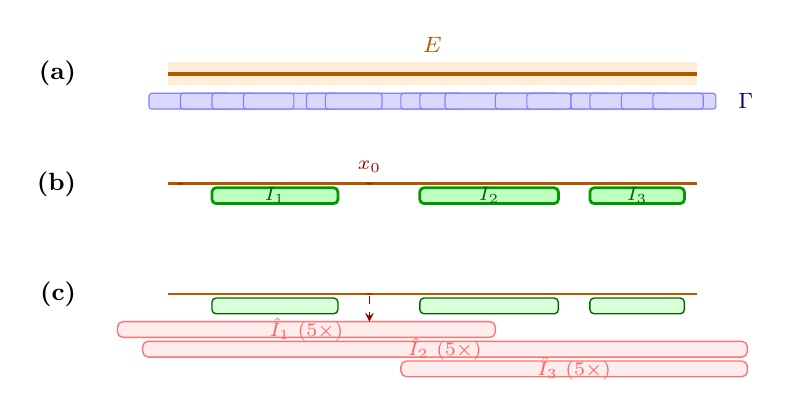
\begin{tikzpicture}[x=8cm, y=1cm, >=stealth]
% --- Row 1: The set E and Vitali intervals ---
\node[anchor=east, font=\small\bfseries] at (-0.05, 0) {(a)};
% E
\fill[orange!15] (0.08,-0.15) rectangle (0.92,0.15);
\draw[orange!70!black, line width=1.5pt] (0.08,0) -- (0.92,0);
\node[above, font=\footnotesize, orange!70!black] at (0.5, 0.15) {$E$};
% Vitali intervals (many overlapping, blue)
\foreach \a/\b in {0.05/0.18, 0.10/0.22, 0.15/0.35, 0.20/0.28, 0.30/0.50, 0.33/0.42, 0.45/0.55, 0.48/0.70, 0.52/0.62, 0.60/0.78, 0.65/0.72, 0.72/0.95, 0.75/0.85, 0.80/0.88, 0.85/0.93} {
  \fill[blue!15, rounded corners=1pt] (\a,-0.45) rectangle (\b,-0.25);
  \draw[blue!50, line width=0.4pt, rounded corners=1pt] (\a,-0.45) rectangle (\b,-0.25);
}
\node[right, font=\footnotesize, blue!50!black] at (0.97, -0.35) {$\Gamma$};

% --- Row 2: Greedy selection ---
\node[anchor=east, font=\small\bfseries] at (-0.05, -1.4) {(b)};
% E again
\draw[orange!70!black, line width=1pt] (0.08,-1.4) -- (0.92,-1.4);
% Selected disjoint intervals (green)
\fill[green!25, rounded corners=1.5pt] (0.15,-1.65) rectangle (0.35,-1.45);
\draw[green!60!black, line width=1pt, rounded corners=1.5pt] (0.15,-1.65) rectangle (0.35,-1.45);
\node[font=\scriptsize, green!40!black] at (0.25,-1.55) {$I_1$};

\fill[green!25, rounded corners=1.5pt] (0.48,-1.65) rectangle (0.70,-1.45);
\draw[green!60!black, line width=1pt, rounded corners=1.5pt] (0.48,-1.65) rectangle (0.70,-1.45);
\node[font=\scriptsize, green!40!black] at (0.59,-1.55) {$I_2$};

\fill[green!25, rounded corners=1.5pt] (0.75,-1.65) rectangle (0.90,-1.45);
\draw[green!60!black, line width=1pt, rounded corners=1.5pt] (0.75,-1.65) rectangle (0.90,-1.45);
\node[font=\scriptsize, green!40!black] at (0.825,-1.55) {$I_3$};
% Uncovered points
\fill[red!70!black] (0.10,-1.4) circle (0.006);
\fill[red!70!black] (0.40,-1.4) circle (0.006);
\node[above, font=\scriptsize, red!60!black] at (0.40,-1.38) {$x_0$};

% --- Row 3: 5x dilations ---
\node[anchor=east, font=\small\bfseries] at (-0.05, -2.8) {(c)};
% E again
\draw[orange!70!black, line width=1pt] (0.08,-2.8) -- (0.92,-2.8);
% Selected intervals (dimmed)
\fill[green!15, rounded corners=1.5pt] (0.15,-3.05) rectangle (0.35,-2.85);
\draw[green!40!black, line width=0.5pt, rounded corners=1.5pt] (0.15,-3.05) rectangle (0.35,-2.85);
\fill[green!15, rounded corners=1.5pt] (0.48,-3.05) rectangle (0.70,-2.85);
\draw[green!40!black, line width=0.5pt, rounded corners=1.5pt] (0.48,-3.05) rectangle (0.70,-2.85);
\fill[green!15, rounded corners=1.5pt] (0.75,-3.05) rectangle (0.90,-2.85);
\draw[green!40!black, line width=0.5pt, rounded corners=1.5pt] (0.75,-3.05) rectangle (0.90,-2.85);
% 5x dilations (pink)
\fill[pink!30, rounded corners=2pt] (0.00,-3.35) rectangle (0.60,-3.15);
\draw[pink!60!red, line width=0.5pt, rounded corners=2pt] (0.00,-3.35) rectangle (0.60,-3.15);
\node[font=\scriptsize, pink!50!red] at (0.30,-3.25) {$\hat{I}_1$ ($5\times$)};

\fill[pink!30, rounded corners=2pt] (0.04,-3.6) rectangle (1.00,-3.4);
\draw[pink!60!red, line width=0.5pt, rounded corners=2pt] (0.04,-3.6) rectangle (1.00,-3.4);
\node[font=\scriptsize, pink!50!red] at (0.52,-3.5) {$\hat{I}_2$ ($5\times$)};

\fill[pink!30, rounded corners=2pt] (0.45,-3.85) rectangle (1.00,-3.65);
\draw[pink!60!red, line width=0.5pt, rounded corners=2pt] (0.45,-3.85) rectangle (1.00,-3.65);
\node[font=\scriptsize, pink!50!red] at (0.725,-3.75) {$\hat{I}_3$ ($5\times$)};
% x_0 covered
\fill[red!70!black] (0.40,-2.8) circle (0.006);
\draw[->, red!60!black, line width=0.4pt, dashed] (0.40,-2.82) -- (0.40,-3.15);
\end{tikzpicture}
\caption{The Vitali covering argument. (a) The set $E$ with many overlapping Vitali intervals $\Gamma$ (blue). (b) Greedy selection produces disjoint $I_1, I_2, I_3$ (green); uncovered points like $x_0$ remain. (c) Each $5\times$ dilation $\hat{I}_j$ (pink) covers the uncovered remainder: any $x_0 \in E \setminus \bigcup I_j$ must land in some $\hat{I}_k$ because the Vitali interval $J \ni x_0$ satisfies $|J| < 2|I_k|$ and $J \cap I_k \neq \emptyset$, forcing $J \subseteq \hat{I}_k$.}
\label{fig:vitali}
\end{figure}

\subsection{Functions of Bounded Variation}

\begin{defbox}[Total Variation and Bounded Variation]
Let $f$ be a real-valued function on $[a, b]$. For a partition $\Delta: a = x_0 < x_1 < \cdots < x_n = b$, define:
\[
v_\Delta = \sum_{j=0}^{n-1} |f(x_{j+1}) - f(x_j)|.
\]
The \textbf{total variation} of $f$ on $[a, b]$ is:
\[
\bigvee_a^b(f) = \sup\{v_\Delta : \Delta \text{ a partition of } [a, b]\}.
\]
If $\bigvee_a^b(f) < \infty$, we say $f$ is of \textbf{bounded variation} on $[a, b]$, and write $f \in BV([a, b])$.
\end{defbox}

\begin{exbox}[Monotone Functions are BV]
If $f$ is increasing on $[a, b]$, then for any partition:
\[
v_\Delta = \sum_{j=0}^{n-1} |f(x_{j+1}) - f(x_j)| = \sum_{j=0}^{n-1} (f(x_{j+1}) - f(x_j)) = f(b) - f(a) \geq 0.
\]
So $\bigvee_a^b(f) = f(b) - f(a) < \infty$. Similarly for decreasing functions.
\end{exbox}

\begin{propbox}[Differentiable Functions with Bounded Derivative are BV]
If $f$ is differentiable on $[a, b]$ with $|f'(x)| \leq M$ for all $x \in [a, b]$, then $f \in BV([a, b])$.
\end{propbox}

\begin{proof}
By the Mean Value Theorem, $|f(x_{j+1}) - f(x_j)| = |f'(\theta_j)|(x_{j+1} - x_j) \leq M(x_{j+1} - x_j)$. So:
\[
v_\Delta = \sum_{j=0}^{n-1} |f(x_{j+1}) - f(x_j)| \leq M \sum_{j=0}^{n-1} (x_{j+1} - x_j) = M(b - a).
\]
Hence $\bigvee_a^b(f) \leq M(b - a) < \infty$.
\end{proof}

\begin{exbox}[A Continuous Function Not in BV]
Define $f(x) = \sqrt{x}\sin(\pi/x)$ for $0 < x \leq 1$ and $f(0) = 0$. Then $f$ is continuous on $[0, 1]$ but $f \notin BV([0, 1])$: the oscillations near $0$ accumulate enough variation to make $\bigvee_0^1(f) = \infty$.
\end{exbox}

\begin{propbox}[Properties of BV Functions]
\begin{enumerate}[label=(\roman*)]
\item If $f \in BV([a, b])$, then $f$ is bounded on $[a, b]$.
\item If $f, g \in BV([a, b])$ and $c_1, c_2 \in \mathbb{R}$, then $c_1 f + c_2 g \in BV([a, b])$, with:
\[
\bigvee_a^b(cf) = |c|\,\bigvee_a^b(f), \qquad \bigvee_a^b(f + g) \leq \bigvee_a^b(f) + \bigvee_a^b(g).
\]
\end{enumerate}
\end{propbox}

\begin{proof}
\textbf{(i)} For any $x \in (a, b]$, the partition $\Delta: a < x < b$ gives:
\[
|f(x) - f(a)| \leq |f(x) - f(a)| + |f(b) - f(x)| = v_\Delta(f) \leq \bigvee_a^b(f) < \infty.
\]
So $|f(x)| \leq |f(a)| + \bigvee_a^b(f) < \infty$ for all $x \in [a, b]$.

\textbf{(ii)} The scaling identity $\bigvee_a^b(cf) = |c|\,\bigvee_a^b(f)$ is immediate. For the triangle inequality, let $\Delta$ be any partition:
\[
v_\Delta(f + g) = \sum_{i=0}^{n-1} |(f + g)(x_{i+1}) - (f + g)(x_i)| \leq \sum_{i=0}^{n-1} |f(x_{i+1}) - f(x_i)| + \sum_{i=0}^{n-1} |g(x_{i+1}) - g(x_i)| = v_\Delta(f) + v_\Delta(g).
\]
Taking the supremum over $\Delta$: $\bigvee_a^b(f + g) \leq \bigvee_a^b(f) + \bigvee_a^b(g) < \infty$.
\end{proof}

\begin{propbox}[Additivity of Total Variation]
Let $f \in BV([a, b])$ and $a < c < b$. Then:
\[
\bigvee_a^b(f) = \bigvee_a^c(f) + \bigvee_c^b(f).
\]
\end{propbox}

\begin{proof}
\textbf{($\geq$):} For any $\varepsilon > 0$, choose a partition $\Delta_1$ of $[a, c]$ with $v_{\Delta_1}(f) > \bigvee_a^c(f) - \varepsilon$, and a partition $\Delta_2$ of $[c, b]$ with $v_{\Delta_2}(f) > \bigvee_c^b(f) - \varepsilon$. Then $\Delta = \Delta_1 \cup \Delta_2$ is a partition of $[a, b]$ with:
\[
v_\Delta(f) = v_{\Delta_1}(f) + v_{\Delta_2}(f) > \bigvee_a^c(f) + \bigvee_c^b(f) - 2\varepsilon.
\]
Since $v_\Delta(f) \leq \bigvee_a^b(f)$, letting $\varepsilon \to 0$ gives $\bigvee_a^b(f) \geq \bigvee_a^c(f) + \bigvee_c^b(f)$.

\textbf{($\leq$):} For any $\varepsilon > 0$, choose a partition $\Delta: a = x_0 < x_1 < \cdots < x_n = b$ with $v_\Delta(f) > \bigvee_a^b(f) - \varepsilon$. Let $\Delta' = \Delta \cup \{c\}$ (refine by adding $c$). Observe that $v_{\Delta'}(f) \geq v_\Delta(f)$ (refining a partition can only increase the variation, since $|f(x_{i+1}) - f(x_i)| \leq |f(x_{i+1}) - f(c)| + |f(c) - f(x_i)|$ by the triangle inequality).

The partition $\Delta'$ splits into $\Delta_1$ (the points $\leq c$) and $\Delta_2$ (the points $\geq c$):
\[
v_{\Delta'}(f) = v_{\Delta_1}(f) + v_{\Delta_2}(f) \leq \bigvee_a^c(f) + \bigvee_c^b(f).
\]
So $\bigvee_a^b(f) - \varepsilon < v_\Delta(f) \leq v_{\Delta'}(f) \leq \bigvee_a^c(f) + \bigvee_c^b(f)$. Letting $\varepsilon \to 0$ gives $\bigvee_a^b(f) \leq \bigvee_a^c(f) + \bigvee_c^b(f)$.
\end{proof}

\begin{corbox}[The Variation Function is Increasing]
If $f \in BV([a,b])$, then the function $T(x) = \bigvee_a^x(f)$ is increasing on $[a, b]$.
\end{corbox}

\begin{proof}
For $a \leq x_1 < x_2 \leq b$, by additivity: $\bigvee_a^{x_2}(f) = \bigvee_a^{x_1}(f) + \bigvee_{x_1}^{x_2}(f) \geq \bigvee_a^{x_1}(f)$.
\end{proof}

\begin{thmbox}[Jordan Decomposition Theorem]
Let $f \in BV([a, b])$. Then there exist increasing functions $g, h$ on $[a, b]$ such that $f(x) = g(x) - h(x)$ for all $x \in [a, b]$.

Conversely, $f \in BV([a, b])$ if and only if $f$ is the difference of two increasing functions.
\end{thmbox}

\begin{proof}
\textbf{($\Rightarrow$)} Let $g(x) = \bigvee_a^x(f)$ and $h(x) = \bigvee_a^x(f) - f(x)$. Then $g$ is increasing (by the corollary above). We show $h$ is increasing: for $a \leq x_1 < x_2 \leq b$,
\begin{align*}
h(x_2) - h(x_1) &= \bigvee_a^{x_2}(f) - f(x_2) - \bigvee_a^{x_1}(f) + f(x_1) = \bigvee_{x_1}^{x_2}(f) - (f(x_2) - f(x_1)).
\end{align*}
Since the partition $\Delta: x_1 < x_2$ gives $|f(x_2) - f(x_1)| \leq \bigvee_{x_1}^{x_2}(f)$, we have $f(x_2) - f(x_1) \leq |f(x_2) - f(x_1)| \leq \bigvee_{x_1}^{x_2}(f)$. Hence $h(x_2) - h(x_1) \geq 0$, so $h$ is increasing.

Since $f(x) = g(x) - h(x)$ with $g, h$ increasing, the decomposition is established.

\textbf{($\Leftarrow$)} If $f = g - h$ with $g, h$ increasing, then $\bigvee_a^b(f) \leq \bigvee_a^b(g) + \bigvee_a^b(h) = (g(b) - g(a)) + (h(b) - h(a)) < \infty$.
\end{proof}

\begin{thmbox}[Total Variation of the Integral Function]
Let $f \in L([a, b])$ and define $F(x) = \int_a^x f(t)\,dt$ for $x \in [a, b]$. Then $F \in BV([a, b])$ and:
\[
\bigvee_a^b(F) = \int_a^b |f(t)|\,dt.
\]
\end{thmbox}

\begin{proof}
\textbf{Upper bound ($\bigvee_a^b(F) \leq \int_a^b |f|\,dt$):} For any partition $\Delta: a = x_0 < x_1 < \cdots < x_n = b$:
\[
v_\Delta(F) = \sum_{i=0}^{n-1} |F(x_{i+1}) - F(x_i)| = \sum_{i=0}^{n-1} \left|\int_{x_i}^{x_{i+1}} f(t)\,dt\right| \leq \sum_{i=0}^{n-1} \int_{x_i}^{x_{i+1}} |f(t)|\,dt = \int_a^b |f(t)|\,dt.
\]
Taking the supremum: $\bigvee_a^b(F) \leq \int_a^b |f(t)|\,dt < \infty$, so $F \in BV$.

\textbf{Lower bound ($\bigvee_a^b(F) \geq \int_a^b |f|\,dt$):}

\textit{Step 1: Step functions.} Assume $f(x) = \sum_{i=0}^{n-1} c_i\,\chi_{[x_i, x_{i+1})}$ is a step function on the partition $\Delta: a = x_0 < \cdots < x_n = b$. Then:
\[
v_\Delta(F) = \sum_{i=0}^{n-1} |F(x_{i+1}) - F(x_i)| = \sum_{i=0}^{n-1} \left|\int_{x_i}^{x_{i+1}} c_i\,dt\right| = \sum_{i=0}^{n-1} |c_i|(x_{i+1} - x_i) = \int_a^b |f(t)|\,dt.
\]
So $\bigvee_a^b(F) \geq v_\Delta(F) = \int_a^b |f|\,dt$.

\textit{Step 2: General $f \in L([a,b])$.} For any $\varepsilon > 0$, by density of step functions in $L^1$, there exists a step function $h$ with $\int_a^b |f(t) - h(t)|\,dt < \varepsilon$. Let $H(x) = \int_a^x h(t)\,dt$. By Step~1, $\bigvee_a^b(H) \geq \int_a^b |h|\,dt$.

By the triangle inequality for total variation and the upper bound:
\[
\int_a^b |f|\,dt \leq \int_a^b |f - h|\,dt + \int_a^b |h|\,dt < \varepsilon + \bigvee_a^b(H) \leq \varepsilon + \bigvee_a^b(F) + \bigvee_a^b(H - F).
\]

Since $H(x) - F(x) = \int_a^x (h(t) - f(t))\,dt$, the upper bound gives $\bigvee_a^b(H - F) \leq \int_a^b |h - f|\,dt < \varepsilon$. Hence:
\[
\int_a^b |f|\,dt < \varepsilon + \bigvee_a^b(F) + \varepsilon = \bigvee_a^b(F) + 2\varepsilon.
\]
Letting $\varepsilon \to 0$: $\int_a^b |f|\,dt \leq \bigvee_a^b(F)$.
\end{proof}


\subsection{Dini Derivatives}

\begin{defbox}[Dini Derivatives]
Let $f$ be a real-valued function on $[a, b]$ and $x_0 \in (a, b)$. The four \textbf{Dini derivatives} of $f$ at $x_0$ are:
\begin{align*}
D^+ f(x_0) &= \limsup_{h \to 0^+} \frac{f(x_0 + h) - f(x_0)}{h}, &\quad D_+ f(x_0) &= \liminf_{h \to 0^+} \frac{f(x_0 + h) - f(x_0)}{h}, \\[4pt]
D^- f(x_0) &= \limsup_{h \to 0^+} \frac{f(x_0) - f(x_0 - h)}{h}, &\quad D_- f(x_0) &= \liminf_{h \to 0^+} \frac{f(x_0) - f(x_0 - h)}{h}.
\end{align*}
\end{defbox}

\begin{rembox}[Relationship to Differentiability]
By definition, $D^+ \geq D_+$ and $D^- \geq D_-$ always hold. If $D^+ f(x_0) \leq D_- f(x_0)$ and $D^- f(x_0) \leq D_+ f(x_0)$, then all four Dini derivatives are sandwiched:
\[
D_+ \leq D^+ \leq D_- \leq D^- \leq D_+,
\]
which forces $D^+ = D_+ = D^- = D_-$, i.e., $f$ is differentiable at $x_0$.

Equivalently: $f$ is \textit{not} differentiable at $x_0$ iff $D^+ > D_-$ or $D^- > D_+$ at $x_0$. In other words, some upper Dini derivative strictly exceeds the corresponding lower one.
\end{rembox}

\subsection{Lebesgue's Theorem on Differentiability of Monotone Functions}

\begin{thmbox}[Lebesgue's Differentiation Theorem for Monotone Functions]
Let $f$ be a monotone increasing function on $[a, b]$. Then:
\begin{enumerate}[label=(\roman*)]
\item $f$ is differentiable a.e.\ on $(a, b)$.
\item $f' \geq 0$ a.e., and $f' \in L([a, b])$ (i.e., $f'$ is integrable).
\item $\displaystyle\int_a^b f'(x)\,dx \leq f(b) - f(a)$.
\end{enumerate}
\end{thmbox}

\begin{rembox}
The inequality in (iii) can be strict: for the Cantor function (``devil's staircase''), $f$ is increasing and continuous on $[0,1]$ with $f(0) = 0$, $f(1) = 1$, but $f' = 0$ a.e., so $\int_0^1 f'\,dx = 0 < 1 = f(1) - f(0)$. A similar statement holds for decreasing functions.
\end{rembox}

\begin{proof}[Proof of (i): A.E.\ Differentiability]
Let $f$ be increasing on $[a, b]$. Define the ``bad'' sets:
\begin{align*}
E_1 &= \{x \in (a, b) : D^+ f(x) > D_- f(x)\}, \\
E_2 &= \{x \in (a, b) : D^- f(x) > D_+ f(x)\}.
\end{align*}

We show $m(E_1) = m(E_2) = 0$. If $x_0 \in (a, b) \setminus (E_1 \cup E_2)$, then $D^+ f(x_0) \leq D_- f(x_0)$ and $D^- f(x_0) \leq D_+ f(x_0)$, which forces all four Dini derivatives to be equal (as argued in the remark above), so $f$ is differentiable at $x_0$.

\textbf{Showing $m(E_1) = 0$.} Write $E_1$ as a countable union:
\[
E_1 = \bigcup_{\substack{r, s \in \mathbb{Q} \\ r > s}} A_{r,s}, \qquad A_{r,s} = \{x \in (a, b) : D^+ f(x) > r > s > D_- f(x)\}.
\]
It suffices to show $m(A_{r,s}) = 0$ for each fixed $r > s$ rational.

Fix $r, s \in \mathbb{Q}$ with $r > s$. Let $A = A_{r,s}$. Suppose for contradiction that $m^*(A) > 0$.

\textbf{Step 1: Apply Vitali to the $D_-$ condition.}

For any $\varepsilon > 0$, choose an open set $G \supseteq A$ with $m(G) < (1 + \varepsilon)\,m^*(A)$. Since $D_- f(x) < s$ for all $x \in A$, for each $x_0 \in A$ there exist arbitrarily small $h_j > 0$ such that:
\[
\frac{f(x_0) - f(x_0 - h_j)}{h_j} < s, \quad \text{i.e.,} \quad f(x_0) - f(x_0 - h_j) < s\,h_j.
\]
The collection $\Gamma = \{[x_0 - h_j, x_0] : x_0 \in A,\; [x_0 - h_j, x_0] \subseteq G,\; h_j > 0\}$ is a Vitali covering of $A$. By the Vitali Covering Theorem, there exist finitely many disjoint intervals $J_1 = [y_1, y_1 + h_1'], \ldots, J_p = [y_p, y_p + h_p']$ in $\Gamma$ with:
\[
m^*\!\left(A \setminus \bigcup_{j=1}^{p} J_j\right) < \varepsilon.
\]

Let $B = A \cap \bigcup_{j=1}^{p} J_j$, so $m^*(B) \geq m^*(A) - \varepsilon$.

Each $J_j$ has endpoint $y_j + h_j' \in A$ and satisfies $f(y_j + h_j') - f(y_j) < s\,h_j'$. Therefore:
\[
\sum_{j=1}^{p} \bigl(f(y_j + h_j') - f(y_j)\bigr) < s \sum_{j=1}^{p} h_j' = s \sum_{j=1}^{p} |J_j|.  \tag{$*$}
\]

\textbf{Step 2: Apply Vitali to the $D^+$ condition.}

For each $x \in B$, $x$ lies in some $J_j$, and $D^+ f(x) > r$. So there exist arbitrarily small $h > 0$ with $[x, x+h] \subseteq \bigcup_{j=1}^{p} J_j$ and:
\[
\frac{f(x + h) - f(x)}{h} > r.
\]
The collection $\Gamma_1 = \{[x, x+h] : x \in B,\; [x,x+h] \subseteq \bigcup_{j=1}^p J_j,\; h > 0,\; f(x+h)-f(x) > rh\}$ is a Vitali covering of $B$. By Vitali, there exist disjoint $I_1 = [x_1 - k_1, x_1], \ldots, I_q = [x_q - k_q, x_q]$ in $\Gamma_1$ with $m^*(B \setminus \bigcup I_i) < \varepsilon$. Each satisfies $f(x_i) - f(x_i - k_i) > r\,k_i$, so:
\[
\sum_{i=1}^{q} r\,k_i < \sum_{i=1}^{q} \bigl(f(x_i) - f(x_i - k_i)\bigr).  \tag{$**$}
\]

\textbf{Step 3: Compare the two bounds.}

Since each $I_i \subseteq \bigcup_j J_j$ and the $\{J_j\}$ are disjoint, the intervals $\{I_i\}$ that fall inside a given $J_j$ are disjoint subintervals of $J_j$. By monotonicity of $f$, the sum of $f(x_i) - f(x_i - k_i)$ over those $I_i \subseteq J_j$ is at most $f(y_j + h_j') - f(y_j)$ (telescoping within $J_j$). Therefore:
\[
\sum_{i=1}^{q} \bigl(f(x_i) - f(x_i - k_i)\bigr) \leq \sum_{j=1}^{p} \bigl(f(y_j + h_j') - f(y_j)\bigr).
\]

Combining ($*$) and ($**$):
\[
r \sum_{i=1}^{q} k_i < \sum_{j=1}^{p} \bigl(f(y_j + h_j') - f(y_j)\bigr) < s \sum_{j=1}^{p} h_j'.
\]

Now $\sum k_i = m(\bigcup I_i)$ and $\sum h_j' = m(\bigcup J_j) \leq m(G) < (1+\varepsilon)\,m^*(A)$. Also $m^*(B) \geq m^*(A) - \varepsilon$ and $m^*(B \setminus \bigcup I_i) < \varepsilon$, so $\sum k_i \geq m^*(B) - \varepsilon \geq m^*(A) - 2\varepsilon$.

Therefore:
\[
r\,(m^*(A) - 2\varepsilon) \leq r \sum k_i < s(1 + \varepsilon)\,m^*(A).
\]

Letting $\varepsilon \to 0$: $r\,m^*(A) \leq s\,m^*(A)$. Since $r > s$, this gives $m^*(A) \leq 0$, contradicting $m^*(A) > 0$.

Hence $m(A_{r,s}) = 0$ for all $r > s$, so $m(E_1) = 0$. The proof that $m(E_2) = 0$ is similar (swap the roles of left and right).
\end{proof}

\begin{proof}[Proof of (iii): The Integral Inequality]
Extend $f$ by setting $f(x) = f(b)$ for $x > b$. Define the difference quotients:
\[
f_n(x) = \frac{f(x + 1/n) - f(x)}{1/n} = n\!\left(f\!\left(x + \tfrac{1}{n}\right) - f(x)\right).
\]

Since $f$ is differentiable a.e.\ (by (i)), $\lim_{n \to \infty} f_n(x) = f'(x)$ for a.e.\ $x \in (a, b)$. Since $f$ is increasing, $f_n(x) \geq 0$ for all $x \in [a, b]$.

By Fatou's lemma:
\[
\int_a^b f'(x)\,dx = \int_a^b \liminf_{n \to \infty} f_n(x)\,dx \leq \liminf_{n \to \infty} \int_a^b f_n(x)\,dx.
\]

We compute $\int_a^b f_n(x)\,dx$:
\begin{align*}
\int_a^b f_n(x)\,dx &= n\!\left(\int_a^b f\!\left(x + \tfrac{1}{n}\right)\!dx - \int_a^b f(x)\,dx\right) = n\!\left(\int_{a+1/n}^{b+1/n} f(t)\,dt - \int_a^b f(x)\,dx\right) \\
&= n\!\left(\int_b^{b+1/n} f(t)\,dt - \int_a^{a+1/n} f(t)\,dt\right).
\end{align*}

Since $f$ is increasing, $f(t) \geq f(b)$ for $t \in [b, b+1/n]$ (using the extension $f(t) = f(b)$ for $t > b$, so actually $f(t) = f(b)$), and $f(t) \leq f(a + 1/n)$ for $t \in [a, a+1/n]$. More precisely:
\[
\int_b^{b+1/n} f(t)\,dt = f(b) \cdot \frac{1}{n}, \qquad \int_a^{a+1/n} f(t)\,dt \geq f(a) \cdot \frac{1}{n}.
\]

Therefore:
\[
\int_a^b f_n(x)\,dx \leq n\!\left(\frac{f(b)}{n} - \frac{f(a)}{n}\right) = f(b) - f(a).
\]

Combining: $\int_a^b f'(x)\,dx \leq \liminf_{n \to \infty} \int_a^b f_n\,dx \leq f(b) - f(a)$.
\end{proof}

\begin{proof}[Proof of (ii): Integrability of $f'$]
Since $f$ is increasing, $f' \geq 0$ wherever it exists. The integral inequality (iii) gives $\int_a^b f'\,dx \leq f(b) - f(a) < \infty$, so $f' \in L([a, b])$. In particular, $f'$ is finite a.e.\ (integrability implies a.e.\ finiteness).
\end{proof}

\begin{corbox}[BV Functions are Differentiable A.E.]
Let $f \in BV([a, b])$. Then $f$ is differentiable a.e.\ on $(a, b)$, and $f' \in L([a, b])$.
\end{corbox}

\begin{proof}
By the Jordan Decomposition Theorem, $f = g - h$ where $g, h$ are increasing on $[a, b]$. By Lebesgue's theorem, $g$ and $h$ are each differentiable a.e.\ on $(a, b)$, with $g', h' \in L([a, b])$. Hence $f$ is differentiable a.e.\ with $f' = g' - h' \in L([a, b])$.
\end{proof}

\subsection{The Fundamental Theorem of Calculus: What Goes Wrong?}

\begin{rembox}[The Central Question Revisited]
For $f: [a, b] \to \mathbb{R}$, under what assumptions do we have:
\[
f(x) - f(a) = \int_a^x f'(t)\,dt \qquad \text{for all } x \in [a, b]? \tag{$*$}
\]
If ($*$) holds, then $f(x) = f(a) + \int_a^x f'(t)\,dt$, and the integral function $G(x) = \int_a^x f'(t)\,dt$ is in $BV([a, b])$ (by the Total Variation Theorem). So $f \in BV([a, b])$ is \textit{necessary} for ($*$).

\textbf{Question}: Is $f \in BV([a, b])$ \textit{sufficient} for ($*$)?

\textbf{Answer}: \textbf{No.} The Cantor function provides a counterexample.
\end{rembox}

\begin{exbox}[The Cantor Function (Devil's Staircase)]
The \textbf{Cantor set} $C \subseteq [0, 1]$ is obtained by repeatedly removing middle thirds: $C = \bigcap_{n=0}^{\infty} C_n$ where $C_0 = [0,1]$, $C_1 = [0, 1/3] \cup [2/3, 1]$, etc. The set $C$ is closed, uncountable, and has $m(C) = 0$.

The \textbf{Cantor function} $\varphi: [0, 1] \to [0, 1]$ is defined via the ternary expansion: for $x \in C$, write $x = \sum_{i=1}^{\infty} 2a_i / 3^i$ (with $a_i \in \{0, 1\}$), and set $\varphi(x) = \sum_{i=1}^{\infty} a_i / 2^i$. Extend $\varphi$ to $[0, 1]$ by constancy on each removed interval. Then:

\begin{enumerate}[label=(\roman*)]
\item $\varphi$ is continuous and increasing on $[0, 1]$, so $\varphi \in BV([0, 1])$.
\item $\varphi(0) = 0$ and $\varphi(1) = 1$.
\item $\varphi'(x) = 0$ for all $x \in [0, 1] \setminus C$, i.e., $\varphi' = 0$ a.e.\ (since $m(C) = 0$).
\end{enumerate}

Therefore:
\[
\int_0^1 \varphi'(t)\,dt = 0 \neq 1 = \varphi(1) - \varphi(0).
\]
The FTC ($*$) fails for $\varphi$, even though $\varphi \in BV$. The function ``gains value'' entirely on the Cantor set, which has measure zero --- invisible to the Lebesgue integral.
\end{exbox}

\begin{rembox}
This shows that BV is not sufficient for the FTC. The missing condition is \textbf{absolute continuity}.
\end{rembox}

\begin{defbox}[Absolute Continuity]
A function $f: [a, b] \to \mathbb{R}$ is \textbf{absolutely continuous} on $[a, b]$ (written $f \in AC([a, b])$) if for every $\varepsilon > 0$ there exists $\delta > 0$ such that for any finite collection of mutually disjoint subintervals $\{(a_k, b_k)\}_{k=1}^{n}$ of $[a, b]$:
\[
\sum_{k=1}^{n} (b_k - a_k) < \delta \implies \sum_{k=1}^{n} |f(b_k) - f(a_k)| < \varepsilon.
\]
\end{defbox}

\begin{rembox}[Comparison with Uniform Continuity]
Taking $n = 1$, absolute continuity implies uniform continuity. The converse is false: the Cantor function $\varphi$ is uniformly continuous on $[0, 1]$ (continuous on a compact set) but \textit{not} absolutely continuous --- the Cantor set $C$ has $m(C) = 0$, so it can be covered by disjoint intervals of arbitrarily small total length, yet $\varphi$ gains all its value on $C$.

The hierarchy of regularity is:
\[
\text{absolutely continuous} \implies \text{BV} \implies \text{differentiable a.e.}
\]
\[
\text{absolutely continuous} \implies \text{uniformly continuous} \implies \text{continuous.}
\]
None of the reverse implications hold.
\end{rembox}

\subsection{Properties of Absolutely Continuous Functions}

\begin{propbox}[Basic Properties of AC Functions]
\begin{enumerate}[label=(\roman*)]
\item If $f \in AC([a, b])$, then $f$ is continuous on $[a, b]$.
\item If $f, g \in AC([a, b])$ and $c_1, c_2 \in \mathbb{R}$, then $c_1 f + c_2 g \in AC([a, b])$.
\item If $f \in \operatorname{Lip}([a, b])$ (i.e., $|f(x) - f(y)| \leq M|x - y|$ for all $x, y \in [a, b]$), then $f \in AC([a, b])$.
\end{enumerate}
\end{propbox}

\begin{proof}
\textbf{(i)} Taking $n = 1$ in the AC definition: for every $\varepsilon > 0$, there exists $\delta > 0$ such that $|y - x| < \delta$ implies $|f(y) - f(x)| < \varepsilon$. This is exactly uniform continuity, which implies continuity.

\textbf{(ii)} Given $\varepsilon > 0$, choose $\delta_f, \delta_g > 0$ from the AC condition for $f$ and $g$ respectively (with $\varepsilon$ replaced by $\varepsilon/(2\max(|c_1|, 1))$ and $\varepsilon/(2\max(|c_2|, 1))$). Let $\delta = \min(\delta_f, \delta_g)$. For any disjoint intervals $(x_j, y_j) \subseteq (a, b)$ with $\sum (y_j - x_j) < \delta$:
\[
\sum_{j=1}^{p} |c_1 f(y_j) + c_2 g(y_j) - c_1 f(x_j) - c_2 g(x_j)| \leq |c_1| \sum |f(y_j) - f(x_j)| + |c_2| \sum |g(y_j) - g(x_j)| < \varepsilon.
\]

\textbf{(iii)} If $f \in \operatorname{Lip}([a, b])$ with constant $M$, then for any disjoint intervals with $\sum (y_j - x_j) < \delta$:
\[
\sum_{j=1}^{p} |f(y_j) - f(x_j)| \leq M \sum_{j=1}^{p} |y_j - x_j| < M\delta.
\]
Taking $\delta = \varepsilon/M$ gives $f \in AC([a, b])$.
\end{proof}

\begin{thmbox}[The Integral Function is Absolutely Continuous]
If $g \in L([a, b])$, then $G(x) = \int_a^x g(t)\,dt$ is in $AC([a, b])$.
\end{thmbox}

\begin{proof}
This is a direct consequence of the absolute continuity of the Lebesgue integral (Section~16): for every $\varepsilon > 0$, there exists $\delta > 0$ such that $m(A) < \delta$ implies $\int_A |g|\,dt < \varepsilon$. For disjoint intervals $(x_j, y_j)$ with $\sum (y_j - x_j) < \delta$, the set $A = \bigcup_j (x_j, y_j)$ has $m(A) < \delta$, so:
\[
\sum_{j=1}^{p} |G(y_j) - G(x_j)| = \sum_{j=1}^{p} \left|\int_{x_j}^{y_j} g(t)\,dt\right| \leq \sum_{j=1}^{p} \int_{x_j}^{y_j} |g(t)|\,dt = \int_A |g|\,dt < \varepsilon. \qedhere
\]
\end{proof}

\subsection{The Fundamental Theorem of Calculus for Lebesgue Integrals}

\begin{thmbox}[The Fundamental Theorem of Calculus for Lebesgue Integrals]
Let $f: [a, b] \to \mathbb{R}$. Then the following are equivalent:
\begin{enumerate}[label=(\roman*)]
\item $f$ is absolutely continuous on $[a, b]$.
\item $f$ is differentiable a.e., $f' \in L([a, b])$, and $f(x) - f(a) = \int_a^x f'(t)\,dt$ for all $x \in [a, b]$.
\end{enumerate}
\end{thmbox}

\begin{proof}[Proof of the Fundamental Theorem of Calculus]\leavevmode

\textbf{(ii) $\boldsymbol{\Rightarrow}$ (i):} Assume $f$ is differentiable a.e., $f' \in L([a, b])$, and $f(x) - f(a) = \int_a^x f'(t)\,dt$ for all $x$. Then $f(x) = f(a) + \int_a^x f'(t)\,dt$. Since $f' \in L([a,b])$, the function $x \mapsto \int_a^x f'(t)\,dt$ is in $AC([a, b])$ by the theorem above (integral functions are AC). Adding the constant $f(a)$ preserves absolute continuity (property~(ii)). Hence $f \in AC([a, b])$.

\textbf{(i) $\boldsymbol{\Rightarrow}$ (ii):} Assume $f \in AC([a, b])$. Then $f \in BV([a, b])$ (AC $\implies$ BV, proved below), so $f$ is differentiable a.e.\ on $(a, b)$ with $f' \in L([a, b])$ (by the BV differentiability corollary). It remains to show $f(x) - f(a) = \int_a^x f'(t)\,dt$ for all $x \in [a, b]$.

Define $F(x) = f(x) - f(a) - \int_a^x f'(t)\,dt$. Since $f \in AC([a, b])$ and $\int_a^x f'(t)\,dt \in AC([a, b])$ (by the theorem above: integral functions are AC), and $AC$ is closed under linear combinations (property~(ii)), we have $F \in AC([a, b])$.

Moreover, $F'(x) = f'(x) - f'(x) = 0$ a.e.\ on $(a, b)$ (using the fact that $(\int_a^x f'\,dt)' = f'(x)$ a.e., proved in the next subsection).

By the lemma on non-constant functions with zero derivative (Section~18.12), if $F$ were not constant, then $F$ would not be absolutely continuous. But $F \in AC([a, b])$, so $F$ must be constant. Since $F(a) = f(a) - f(a) - 0 = 0$, we conclude $F(x) = 0$ for all $x \in [a, b]$, i.e.:
\[
f(x) - f(a) = \int_a^x f'(t)\,dt \qquad \forall\, x \in [a, b]. \qedhere
\]
\end{proof}

\begin{corbox}[Term-by-Term Differentiation of AC Series]
Let $\{g_k\}_{k \in \mathbb{N}}$ be a sequence of $AC$ functions on $[a, b]$, and assume $\sum_{k=1}^{\infty} g_k(c)$ converges for some $c \in [a, b]$ and $\sum_{k=1}^{\infty} \int_a^b |g_k'(x)|\,dx < \infty$. Then:
\begin{enumerate}[label=(\roman*)]
\item $\sum_{k=1}^{\infty} g_k(x)$ converges for all $x \in [a, b]$.
\item $\sum_{k=1}^{\infty} g_k \in AC([a, b])$.
\item $\left(\sum_{k=1}^{\infty} g_k(x)\right)' = \sum_{k=1}^{\infty} g_k'(x)$ a.e.\ on $(a, b)$.
\end{enumerate}
\end{corbox}

\begin{proof}
Since $g_k \in AC$, the FTC gives $g_k(x) = g_k(c) + \int_c^x g_k'(t)\,dt$. Therefore:
\[
\sum_{k=1}^{\infty} g_k(x) = \sum_{k=1}^{\infty} g_k(c) + \int_c^x \sum_{k=1}^{\infty} g_k'(t)\,dt,
\]
where the interchange of sum and integral is justified as follows.

\textbf{(i)} Since $\sum |g_k'| < \infty$ a.e.\ (by $\sum \int |g_k'| < \infty$ and MCT), $\sum g_k'$ converges absolutely a.e. By DCT (with dominating function $\sum |g_k'| \in L$):
\[
\lim_{n \to \infty} \int_c^x \sum_{k=1}^{n} g_k'(t)\,dt = \int_c^x \sum_{k=1}^{\infty} g_k'(t)\,dt.
\]
Since $\sum g_k(c)$ converges, $\sum g_k(x)$ converges for all $x$.

\textbf{(ii)} $\sum g_k(x) = \sum g_k(c) + \int_c^x h(t)\,dt$ where $h = \sum g_k' \in L([a, b])$. The integral function of an $L$ function is $AC$ (integral functions are AC), and adding a constant preserves $AC$. So $\sum g_k \in AC$.

\textbf{(iii)} Differentiating: $(\sum g_k)' = h' = (\int_c^x h\,dt)' = h(x) = \sum g_k'(x)$ a.e.
\end{proof}

\begin{thmbox}[Lebesgue Decomposition of Increasing Functions]
Let $f$ be an increasing function on $[a, b]$. Then $f = g + h$, where:
\begin{enumerate}[label=(\roman*)]
\item $g$ is increasing and absolutely continuous on $[a, b]$,
\item $h$ is increasing on $[a, b]$ with $h' = 0$ a.e.
\end{enumerate}
\end{thmbox}

\begin{proof}
By Lebesgue's differentiation theorem, $f' \geq 0$ a.e.\ and $f' \in L([a, b])$. Define:
\[
g(x) = f(a) + \int_a^x f'(t)\,dt, \qquad h(x) = f(x) - g(x).
\]

$g$ is increasing (since $f' \geq 0$) and $g \in AC$ (integral of an $L$ function). By the FTC, $g' = f'$ a.e.

$h$ is increasing: for $x < y$, $g(y) - g(x) = \int_x^y f' \leq f(y) - f(x)$ (by Lebesgue's integral inequality for increasing functions), so $h(y) - h(x) = (f(y) - f(x)) - (g(y) - g(x)) \geq 0$.

$h' = 0$ a.e.: $h' = f' - g' = f' - f' = 0$ a.e.
\end{proof}

\begin{rembox}
The function $h$ is called the \textbf{singular part} of $f$: it is increasing yet gains all its growth on a set of measure zero ($\{h' > 0\}$ has measure zero). The Cantor function is the prototypical example of a purely singular increasing function.
\end{rembox}

\begin{thmbox}[$AC \implies BV$]
If $f \in AC([a, b])$, then $f \in BV([a, b])$.
\end{thmbox}

\begin{proof}
Take $\varepsilon = 1$ in the AC definition: there exists $\delta_0 > 0$ such that for any disjoint intervals $(x_j, y_j) \subseteq (a, b)$ with $\sum (y_j - x_j) < \delta_0$, we have $\sum |f(y_j) - f(x_j)| \leq 1$.

Divide $[a, b]$ into $n$ subintervals $[c_j, c_{j+1}]$ of length $(b - a)/n < \delta_0$ (choose $n$ large enough). Fix any subinterval $[c_j, c_{j+1}]$ and take any partition $c_j = t_0 < t_1 < \cdots < t_m = c_{j+1}$. The intervals $(t_0, t_1), \ldots, (t_{m-1}, t_m)$ are disjoint in $(a, b)$ with total length:
\[
\sum_{k=0}^{m-1} (t_{k+1} - t_k) = c_{j+1} - c_j = \frac{b-a}{n} < \delta_0.
\]
So the AC condition applies, giving $\sum_{k=0}^{m-1} |f(t_{k+1}) - f(t_k)| \leq 1$. Since this holds for \textit{every} partition of $[c_j, c_{j+1}]$, taking the supremum: $\bigvee_{c_j}^{c_{j+1}}(f) \leq 1$. By additivity of total variation:
\[
\bigvee_a^b(f) = \sum_{j=0}^{n-1} \bigvee_{c_j}^{c_{j+1}}(f) \leq n.
\]
\end{proof}

\begin{rembox}[The Hierarchy]
Summarizing:
\[
\operatorname{Lip}([a,b]) \subsetneq AC([a,b]) \subsetneq BV([a,b]) \cap C([a,b]).
\]
The Cantor function shows $BV \cap C \not\subseteq AC$. The function $\sqrt{x}$ on $[0, 1]$ shows $AC \not\subseteq \operatorname{Lip}$ (it is AC since $\sqrt{x} = \int_0^x \frac{1}{2\sqrt{t}}\,dt$ with $\frac{1}{2\sqrt{t}} \in L$, but $|\sqrt{x}|/|x| \to \infty$).
\end{rembox}

\begin{lembox}[AC on Subintervals]
If $f$ is AC on $[a, b]$ and $[c, d] \subseteq [a, b]$, then $f$ is AC on $[c, d]$.
\end{lembox}

\begin{proof}
Any collection of disjoint intervals in $(c, d)$ is also a collection of disjoint intervals in $(a, b)$, so the same $\delta$ from the AC condition on $[a, b]$ works on $[c, d]$.
\end{proof}

\begin{lembox}[Image Measure Bounded by Total Variation]
If $f$ is continuous on $[c, d]$, then $f((c, d))$ is an interval and $m(f((c, d))) \leq \bigvee_c^d(f)$.
\end{lembox}

\begin{proof}
Since $f$ is continuous, $f((c, d))$ is an interval contained in $[f_{\min}, f_{\max}]$, where $f_{\min}$ and $f_{\max}$ are the minimum and maximum of $f$ on $[c, d]$. So $m(f((c, d))) \leq f_{\max} - f_{\min}$. Let $x_{\min}, x_{\max} \in [c, d]$ be points where $f$ attains its min and max, with $x_{\min} < x_{\max}$ WLOG. The partition $\Delta = \{c, x_{\min}, x_{\max}, d\}$ gives:
\[
f_{\max} - f_{\min} = |f(x_{\max}) - f(x_{\min})| \leq |f(x_{\min}) - f(c)| + |f(x_{\max}) - f(x_{\min})| + |f(d) - f(x_{\max})| = v_\Delta(f) \leq \bigvee_c^d(f).
\]
Hence $m(f((c, d))) \leq \bigvee_c^d(f)$.
\end{proof}

\begin{thmbox}[AC Functions Map Null Sets to Null Sets]
If $f \in AC([a, b])$ and $Z \subseteq [a, b]$ with $m(Z) = 0$, then $m(f(Z)) = 0$.
\end{thmbox}

\begin{proof}
Since $f \in AC([a, b])$, by the FTC, $f' \in L([a, b])$ and $f(x) = f(a) + \int_a^x f'(t)\,dt$. By the first lemma, $f$ is AC on any $[c, d] \subseteq [a, b]$, so $f(x) = f(c) + \int_c^x f'(t)\,dt$ on $[c, d]$. Applying the total variation formula for integral functions (subsection~18.4) to $f' \in L([c, d])$:
\[
\bigvee_c^d(f) = \bigvee_c^d\!\left(f(c) + \int_c^x f'(t)\,dt\right) = \bigvee_c^d\!\left(\int_c^x f'(t)\,dt\right) = \int_c^d |f'(t)|\,dt,
\]
where the first equality holds because a constant does not affect total variation.

Let $\varepsilon > 0$. Since $|f'| \in L([a, b])$, by absolute continuity of the Lebesgue integral, there exists $\delta > 0$ such that for any measurable $E \subseteq [a, b]$ with $m(E) < \delta$:
\[
\int_E |f'(t)|\,dt < \varepsilon.
\]

Since $m(Z) = 0$, there exist countably many open intervals $\{I_k\}_{k=1}^{\infty}$ with $Z \subseteq \bigcup_{k=1}^{\infty} I_k$ and $\sum_{k=1}^{\infty} m(I_k) < \delta$. Let $G = (\bigcup_{k=1}^{\infty} I_k) \cap (a, b)$. Then $G$ is open in $(a, b)$, $Z \setminus \{a, b\} \subseteq G$, and $m(G) < \delta$. Write $G$ as a countable disjoint union of open intervals: $G = \bigcup_{k=1}^{\infty} (a_k, b_k)$.

Since $\{a, b\}$ has measure zero, $m(f(\{a, b\})) = 0$ (finitely many points), so it suffices to show $m(f(Z \setminus \{a, b\})) = 0$. By the second lemma and the total variation identity:
\[
m(f((a_k, b_k))) \leq \bigvee_{a_k}^{b_k}(f) = \int_{a_k}^{b_k} |f'(t)|\,dt.
\]

Therefore:
\[
m(f(Z \setminus \{a, b\})) \leq \sum_{k=1}^{\infty} m(f((a_k, b_k))) \leq \sum_{k=1}^{\infty} \int_{a_k}^{b_k} |f'(t)|\,dt = \int_G |f'(t)|\,dt < \varepsilon.
\]
Since $\varepsilon > 0$ is arbitrary, $m(f(Z)) = 0$.
\end{proof}

\begin{rembox}
This is a strong property of AC functions: they cannot ``spread'' null sets. The Cantor function, by contrast, maps the Cantor set ($m = 0$) onto $[0, 1]$ ($m = 1$) --- another illustration of why $BV \cap C \not\subseteq AC$.
\end{rembox}



\subsection{Measurability Under Continuous and Linear Maps}

\begin{thmbox}[Continuous Maps Preserve Bounded Closed Sets]
Let $T: \mathbb{R}^n \to \mathbb{R}^n$ be a continuous map. Then for every bounded closed set $F \subseteq \mathbb{R}^n$, the image $T(F)$ is bounded and closed.
\end{thmbox}

\begin{proof}
Since $F$ is bounded and closed in $\mathbb{R}^n$, $F$ is compact. Since $T$ is continuous, $T(F)$ is compact. Since $\mathbb{R}^n$ is a metric space, compact subsets are bounded and closed.
\end{proof}

\begin{thmbox}[Continuous Maps Preserving Null Sets Preserve Measurability]
Let $T: \mathbb{R}^n \to \mathbb{R}^n$ be a continuous map. Assume $T$ maps measure-zero sets to measure-zero sets: $m^*(Z) = 0 \implies m^*(T(Z)) = 0$. Then for every $E \in \mathcal{M}(\mathbb{R}^n)$, we have $T(E) \in \mathcal{M}(\mathbb{R}^n)$.
\end{thmbox}

\begin{proof}
Write $E = \bigcup_{m=1}^{\infty} F_m \cup Z$, where each $F_m$ is bounded and closed with $m(F_m) < \infty$, and $m(Z) = 0$. Then $T(E) = \bigcup_{m=1}^{\infty} T(F_m) \cup T(Z)$. By the previous theorem, each $T(F_m)$ is bounded and closed, hence measurable. By hypothesis, $m^*(T(Z)) = 0$, so $T(Z)$ is measurable. A countable union of measurable sets is measurable, so $T(E) \in \mathcal{M}(\mathbb{R}^n)$.
\end{proof}

\begin{thmbox}[Linear Maps Preserve Null Sets]
Let $T: \mathbb{R}^n \to \mathbb{R}^n$ be a linear map. Then $m^*(Z) = 0 \implies m^*(T(Z)) = 0$.
\end{thmbox}

\begin{proof}
\textbf{Case 1: $T$ is not invertible.} Then $\det T = 0$, so $T(\mathbb{R}^n)$ is a proper linear subspace of $\mathbb{R}^n$ (dimension $< n$). A $k$-dimensional subspace of $\mathbb{R}^n$ with $k < n$ has $n$-dimensional Lebesgue measure zero (it is contained in a countable union of ``flat'' rectangles with one side of length $0$). Since $T(Z) \subseteq T(\mathbb{R}^n)$, we have $m^*(T(Z)) = 0$.

\textbf{Case 2: $T$ is invertible.} We show $m(T(R)) = |\!\det T|\,m(R)$ for any rectangle $R$, then use L-coverings.

\textit{Measure of parallelotopes.} Factor $T$ into elementary row operations (which generate all invertible linear maps): scaling one coordinate by $c$ multiplies volume by $|c|$ and determinant by $c$; adding a multiple of one coordinate to another is a shear with determinant $1$ that preserves volume (by Fubini: the cross-sectional area at each height is unchanged); swapping two coordinates has determinant $-1$ and preserves volume. Since both $m(T(\cdot))$ and $|\!\det T|\,m(\cdot)$ are multiplicative under composition, $m(T(R)) = |\!\det T|\,m(R)$.

\textit{Null sets.} For any $\varepsilon > 0$, choose an L-covering $\{R_j\}_{j=1}^{\infty}$ of $Z$ with $\sum m(R_j) < \varepsilon$. Then $\{T(R_j)\}$ covers $T(Z)$, so by subadditivity:
\[
m^*(T(Z)) \leq \sum_{j=1}^{\infty} m(T(R_j)) = |\!\det T| \sum_{j=1}^{\infty} m(R_j) < |\!\det T|\,\varepsilon.
\]
Since $\varepsilon > 0$ is arbitrary, $m^*(T(Z)) = 0$.
\end{proof}

\begin{corbox}[Composition with Invertible Linear Maps Preserves Measurability]
Let $f$ be a measurable function on $\mathbb{R}^n$ and $T: \mathbb{R}^n \to \mathbb{R}^n$ an invertible linear map. Then $f \circ T$ is measurable on $\mathbb{R}^n$.
\end{corbox}

\begin{proof}
For any $\alpha \in \mathbb{R}$:
\[
\{x \in \mathbb{R}^n : (f \circ T)(x) > \alpha\} = (f \circ T)^{-1}((\alpha, \infty)) = T^{-1}(f^{-1}((\alpha, \infty))).
\]
Since $f$ is measurable, $A = f^{-1}((\alpha, \infty)) \in \mathcal{M}(\mathbb{R}^n)$. Since $T^{-1}$ is an invertible linear map (hence continuous and preserving null sets), $T^{-1}(A) \in \mathcal{M}(\mathbb{R}^n)$ by the theorem above. So $f \circ T$ is measurable.
\end{proof}

\begin{propbox}[Measurability of $f(x + t)$ on $\mathbb{R}^2$]
If $f$ is a measurable function on $\mathbb{R}$, then $(x, t) \mapsto f(x + t)$ is a measurable function on $\mathbb{R}^2$.
\end{propbox}

\begin{proof}
Define $F: \mathbb{R}^2 \to \mathbb{R}$ by $F(x, y) = f(x)$. Then $F$ is measurable on $\mathbb{R}^2$: for each $\alpha$, $\{(x,y) : F(x,y) > \alpha\} = \{x : f(x) > \alpha\} \times \mathbb{R}$, which is measurable (product of a measurable set with $\mathbb{R}$).

Define the invertible linear map $T: \mathbb{R}^2 \to \mathbb{R}^2$ by $T(x, t) = (x + t,\; x - t)$, so $T^{-1}(u, v) = ((u+v)/2,\; (u-v)/2)$. Then:
\[
F(T(x, t)) = F(x + t,\; x - t) = f(x + t).
\]
By the corollary above, $F \circ T$ is measurable on $\mathbb{R}^2$.
\end{proof}

\subsection{Differentiating the Integral: $F'(x) = f(x)$ A.E.}

The other direction of the FTC asks: if we \textit{start} with an integrable function and form its integral, can we recover it by differentiating?

\begin{lembox}[Averaging Lemma]
Let $f \in L(\mathbb{R})$. Define the \textbf{average function}:
\[
F_h(x) = \frac{1}{h}\int_0^h f(x + t)\,dt \qquad (h > 0).
\]
Then $\lim_{h \to 0} \int_{\mathbb{R}} |F_h(x) - f(x)|\,dx = 0$, i.e., $F_h \to f$ in $L^1(\mathbb{R})$.
\end{lembox}

\begin{proof}
\textit{$F_h \in L^1(\mathbb{R})$}: By the triangle inequality and Tonelli (swapping the order of integration):
\[
\int_{\mathbb{R}} |F_h(x)|\,dx \leq \frac{1}{h}\int_0^h \int_{\mathbb{R}} |f(x+t)|\,dx\,dt = \frac{1}{h}\int_0^h \|f\|_1\,dt = \|f\|_1 < \infty,
\]
where we used translation invariance ($\int |f(x+t)|\,dx = \int |f(x)|\,dx = \|f\|_1$). So $F_h \in L^1(\mathbb{R})$.

\textit{$\|F_h - f\|_1 \to 0$}: Note:
\[
F_h(x) - f(x) = \frac{1}{h}\int_0^h f(x+t)\,dt - f(x) = \frac{1}{h}\int_0^h \bigl(f(x+t) - f(x)\bigr)\,dt.
\]

Therefore:
\[
\int_{\mathbb{R}} |F_h(x) - f(x)|\,dx \leq \frac{1}{h}\int_0^h \int_{\mathbb{R}} |f(x+t) - f(x)|\,dx\,dt,
\]
where we used the triangle inequality under the integral and swapped the order of integration (justified by Tonelli, since $g(x,t) = |f(x+t) - f(x)|$ is measurable on $\mathbb{R}^2$).

\textit{Measurability of $g$}: By the proposition above, $(x, t) \mapsto f(x+t)$ is measurable on $\mathbb{R}^2$. Since $f(x)$ is also measurable on $\mathbb{R}^2$ (constant in $t$), $g(x, t) = |f(x+t) - f(x)|$ is measurable.

By the average continuity theorem (Section~17), for every $\varepsilon > 0$ there exists $\delta > 0$ such that $|t| < \delta$ implies $\int_{\mathbb{R}} |f(x+t) - f(x)|\,dx < \varepsilon$. So for $0 < h < \delta$:
\[
\int_{\mathbb{R}} |F_h(x) - f(x)|\,dx \leq \frac{1}{h}\int_0^h \varepsilon\,dt = \varepsilon. \qedhere
\]
\end{proof}

\begin{thmbox}[Differentiation of the Integral]
Let $f \in L(\mathbb{R})$. Define $F(x) = \int_a^x f(t)\,dt$. Then $F$ is differentiable a.e.\ and $F'(x) = f(x)$ a.e.
\end{thmbox}

\begin{proof}
By the Averaging Lemma, $F_h \to f$ in $L^1$ as $h \to 0$. In particular, there exists a sequence $h_n \to 0$ such that $F_{h_n} \to f$ pointwise a.e.\ (every $L^1$-convergent sequence has a pointwise a.e.\ convergent subsequence).

But:
\[
F_{h_n}(x) = \frac{1}{h_n}\int_0^{h_n} f(x+t)\,dt = \frac{1}{h_n}\int_x^{x+h_n} f(t)\,dt = \frac{F(x + h_n) - F(x)}{h_n}.
\]

So $\frac{F(x+h_n) - F(x)}{h_n} \to f(x)$ a.e.\ along the sequence $\{h_n\}$.

To promote this to a full derivative (limit as $h \to 0$, not just along a sequence): we already know $F \in BV([a,b])$ (by the Total Variation Theorem), hence $F$ is differentiable a.e.\ (by Lebesgue's theorem). Where $F'(x)$ exists, it must equal $f(x)$ (since the subsequential limit $f(x)$ is the only possible limit). Therefore $F'(x) = f(x)$ a.e.
\end{proof}

\begin{defbox}[Lebesgue Point]
Let $f \in L(\mathbb{R})$ and define $F(x) = \int_a^x f(t)\,dt$. A point $x_0$ is called a \textbf{Lebesgue point} of $f$ if $F'(x_0)$ exists and $F'(x_0) = f(x_0)$, i.e.:
\[
\lim_{h \to 0} \frac{1}{h}\int_0^h f(x_0 + t)\,dt = f(x_0).
\]
The theorem above shows that a.e.\ point is a Lebesgue point of $f$.
\end{defbox}

\begin{rembox}
If $\tilde{F}(x) = f(x) - f(a) - \int_a^x f'(t)\,dt$, then $\tilde{F}$ is differentiable a.e.\ with $\tilde{F}' = f' - f' = 0$ a.e.\ on $(a,b)$. The Cantor function shows $\tilde{F}$ can be non-constant: $\tilde{F} \equiv \varphi$ satisfies $\varphi' = 0$ a.e.\ but $\varphi(1) - \varphi(0) = 1$. So the FTC fails precisely when $\tilde{F}$ is a ``Cantor-like'' component.
\end{rembox}

\subsection{Non-Constant Functions with Zero Derivative Are Not Absolutely Continuous}

\begin{thmbox}
Assume $f$ is differentiable a.e.\ on $(a, b)$ with $f'(x) = 0$ for a.e.\ $x \in (a, b)$, and assume $f$ is not a constant. Then $f$ is not absolutely continuous: there exists $\varepsilon_0 > 0$ such that for every $\delta > 0$, there exist finitely many mutually disjoint subintervals $\{(x_j, y_j)\}_{j=1}^{n}$ of $(a, b)$ with:
\[
\sum_{j=1}^{n} |y_j - x_j| < \delta \qquad \text{but} \qquad \sum_{j=1}^{n} |f(y_j) - f(x_j)| \geq \varepsilon_0.
\]
\end{thmbox}

\begin{proof}
Since $f$ is not constant, there exists $c \in (a, b)$ with $f(c) \neq f(a)$. Let $A = \{x \in (a, c) : f'(x) = 0\}$. Since $f' = 0$ a.e., we have $m([a, c] \setminus A) = 0$, so $m(A) = c - a$.

For every $x_0 \in A$: $f'(x_0) = 0$ means for every $r > 0$, there exists $\delta_0 > 0$ such that for all $0 < h < \delta_0$:
\[
|f(x_0 + h) - f(x_0)| < r\,h.
\]
Define $\Gamma = \{[x, x+h] : x \in A,\; [x, x+h] \subseteq (a, c),\; |f(x+h) - f(x)| < r\,|h|\}$. For any $r > 0$, $\Gamma$ is a Vitali covering of $A$.

By the Vitali Covering Lemma: for every $\delta > 0$, there exist finitely many disjoint intervals $[x_j, x_j + h_j] \in \Gamma$, $j = 1, \ldots, p$, with:
\[
m\!\left(A \setminus \bigcup_{j=1}^{p} [x_j, x_j + h_j]\right) < \delta.
\]
Since $m([a,c] \setminus A) = 0$, this gives $m\!\left([a, c] \setminus \bigcup_{j=1}^{p} [x_j, x_j + h_j]\right) < \delta$.

The intervals $[x_j, x_j + h_j] \subseteq (a,c)$ are disjoint, so $\sum h_j \leq c - a$. Ordering them as $a < x_1 < x_1 + h_1 < x_2 < \cdots < x_p + h_p < c$, the ``gaps'' between them (including the initial and final gaps) have total length:
\[
\sum_{j=0}^{p} |(\text{gaps})| = (c - a) - \sum_{j=1}^{p} h_j.
\]
By the triangle inequality:
\[
|f(c) - f(a)| \leq \sum_{j=0}^{p} |f(\text{gap endpoints})| + \sum_{j=1}^{p} |f(x_j + h_j) - f(x_j)|.
\]
More precisely, the total oscillation of $f$ on $[a, c]$ decomposes as:
\[
|f(c) - f(a)| \leq \sum_{\text{gaps}} |f \text{ change}| + \sum_{j=1}^{p} |f(x_j + h_j) - f(x_j)| < \sum_{\text{gaps}} |f \text{ change}| + r \sum_{j=1}^{p} h_j \leq \sum_{\text{gaps}} |f \text{ change}| + r(c - a).
\]

Take $r = \frac{|f(c) - f(a)|}{2(c - a)}$. Then:
\[
\sum_{\text{gaps}} |f \text{ change}| \geq |f(c) - f(a)| - r(c - a) = \frac{1}{2}|f(c) - f(a)| > 0.
\]

Set $\varepsilon_0 = \frac{1}{2}|f(c) - f(a)|$. The ``gaps'' are finitely many disjoint subintervals of $[a, c]$ whose total length is $< \delta$ (since they form the complement of the Vitali cover), yet the total oscillation of $f$ on these gaps is $\geq \varepsilon_0$. This shows $f$ is not absolutely continuous.
\end{proof}

% ============================================================================
% SECTION 19: NORMED LINEAR SPACES AND L^p SPACES
% ============================================================================

\chapter{$L^p$ Spaces}

\section{Normed Linear Spaces and $L^p$ Spaces}

\subsection{Normed Linear Spaces}

\begin{defbox}[Linear Space]
A set $X$ is called a \textbf{linear space} (or vector space) over $\mathbb{R}$ if for all $v_1, v_2 \in X$ and $c_1, c_2 \in \mathbb{R}$, we have $c_1 v_1 + c_2 v_2 \in X$ (with the usual axioms of vector addition and scalar multiplication).
\end{defbox}

\begin{exbox}[Linear Spaces in This Course]
$\mathbb{R}^n$, $L^1(E)$, $BV([a,b])$, and $AC([a,b])$ are all linear spaces.
\end{exbox}

\begin{defbox}[Norm]
Let $X$ be a linear space. A function $\|\cdot\|: X \to \mathbb{R}$ is called a \textbf{norm} if:
\begin{enumerate}[label=(\roman*)]
\item $\|x\| \geq 0$ for all $x \in X$, and $\|x\| = 0$ if and only if $x = 0$.
\item $\|x + y\| \leq \|x\| + \|y\|$ for all $x, y \in X$ (triangle inequality).
\item $\|cx\| = |c|\,\|x\|$ for all $c \in \mathbb{R}$, $x \in X$ (homogeneity).
\end{enumerate}
The pair $(X, \|\cdot\|)$ is called a \textbf{normed linear space}.
\end{defbox}

\begin{exbox}[Norms on $\mathbb{R}^n$]
For $\mathbf{x} = (x_1, \ldots, x_n) \in \mathbb{R}^n$: $\|\mathbf{x}\|_2 = \left(\sum_{i=1}^{n} x_i^2\right)^{1/2}$ is the Euclidean norm, and $\|\mathbf{x}\|_1 = \sum_{i=1}^{n} |x_i|$ is the $\ell^1$ norm. Both are norms on $\mathbb{R}^n$.
\end{exbox}

\begin{exbox}[Norms on Function Spaces]
$L^1(E)$: $\|f\|_1 = \int_E |f(x)|\,dx$. Then $(L^1(E), \|\cdot\|_1)$ is a normed linear space.

$BV([a,b])$: $\bigvee_a^b(f)$ is a norm on $BV([a,b]) / \{\text{constants}\}$ (since $\bigvee_a^b(f) = 0$ iff $f$ is constant, not necessarily zero).
\end{exbox}

\begin{propbox}[Every Normed Space is a Metric Space]
If $(X, \|\cdot\|)$ is a normed linear space, then $d(x, y) = \|x - y\|$ defines a metric on $X$.
\end{propbox}

\begin{proof}
$d(x, y) = \|x - y\| \geq 0$ with equality iff $x = y$ (property (i)). Symmetry: $d(x, y) = \|x - y\| = \|{-(y - x)}\| = |{-1}|\,\|y - x\| = d(y, x)$. Triangle inequality: $d(x, y) = \|x - y\| = \|(x - z) + (z - y)\| \leq \|x - z\| + \|z - y\| = d(x, z) + d(z, y)$.
\end{proof}

\subsection{Completeness and Banach Spaces}

\begin{defbox}[Convergence and Cauchy Sequences]
Let $(X, \|\cdot\|)$ be a normed linear space. A sequence $\{x_k\}_{k=1}^{\infty} \subseteq X$ \textbf{converges} to $a \in X$ if $\lim_{k \to \infty} \|x_k - a\| = 0$. We write $\lim_{k \to \infty} x_k = a$ in $(X, \|\cdot\|)$.

The sequence is a \textbf{Cauchy sequence} if for every $\varepsilon > 0$, there exists $N > 0$ such that $\|x_k - x_m\| < \varepsilon$ for all $k, m > N$.
\end{defbox}

\begin{defbox}[Banach Space]
A normed linear space $(X, \|\cdot\|)$ is \textbf{complete} if every Cauchy sequence in $X$ converges to a limit in $X$. A complete normed linear space is called a \textbf{Banach space}.
\end{defbox}

\begin{exbox}[Banach Spaces]
$(\mathbb{R}^n, \|\cdot\|_1)$ and $(\mathbb{R}^n, \|\cdot\|_2)$ are Banach spaces (completeness of $\mathbb{R}^n$ in any norm). The Riesz--Fischer theorem states that $(L^1(E), \|\cdot\|_1)$ is a Banach space.
\end{exbox}

\subsection{$L^p$ Spaces}

\begin{defbox}[$L^p$ Space]
Let $E \in \mathcal{M}(\mathbb{R}^n)$ and $1 \leq p < \infty$. A measurable function $f$ on $E$ belongs to $L^p(E)$ if:
\[
\int_E |f(x)|^p\,dx < \infty.
\]
(Note: $|f(x)|^p$ is still measurable since $t \mapsto |t|^p$ is continuous.) We define the $L^p$ \textbf{norm} of $f$ by:
\[
\|f\|_{L^p(E)} = \|f\|_p = \left(\int_E |f(x)|^p\,dx\right)^{1/p}.
\]
\end{defbox}

\begin{rembox}
When $p = 1$, this recovers $L^1(E)$ with $\|f\|_1 = \int_E |f|\,dx$. The $L^p$ spaces for $p > 1$ are important in functional analysis and PDE theory. The key results (not proved in this course) are:

H\"older's inequality: $\|fg\|_1 \leq \|f\|_p \|g\|_q$ where $1/p + 1/q = 1$.

Minkowski's inequality: $\|f + g\|_p \leq \|f\|_p + \|g\|_p$ (the triangle inequality for $\|\cdot\|_p$).

Riesz--Fischer theorem: $(L^p(E), \|\cdot\|_p)$ is a Banach space for all $1 \leq p < \infty$.

The case $p = 2$ is especially important: $L^2(E)$ is a Hilbert space with inner product $\langle f, g \rangle = \int_E f(x)\,g(x)\,dx$, and $\|f\|_2 = \langle f, f \rangle^{1/2}$.
\end{rembox}

\begin{exbox}[$L^p$ Membership Depends on $p$]
Let $E = (0, 1)$ and $g(x) = 1/\sqrt{x}$. Then $g \in L^p((0,1))$ iff $\int_0^1 x^{-p/2}\,dx < \infty$ iff $p/2 < 1$ iff $p < 2$. So $g \in L^1$ but $g \notin L^2$.

Let $E = (0, 1)$ and $f(x) = \ln(1/x)$. Then $f \in L^\infty((0,1))$? No: $\ln(1/x) \to \infty$ as $x \to 0^+$. But $\int_0^1 |\ln(1/x)|^p\,dx < \infty$ for all $1 \leq p < \infty$ (since $|\ln(1/x)| \leq c\,|x|^{-\alpha}$ for any $\alpha > 0$).
\end{exbox}

\subsection{$L^\infty$ and the Essential Supremum}

\begin{defbox}[$L^\infty$ Space and Essential Supremum]
Let $E \in \mathcal{M}(\mathbb{R}^n)$ and $f$ a measurable function on $E$. We say $f \in L^\infty(E)$ if there exists a constant $M > 0$ such that $|f(x)| \leq M$ for a.e.\ $x \in E$. Such $f$ is called \textbf{essentially bounded}.

The \textbf{essential supremum} of $|f|$ is:
\[
\|f\|_\infty = \|f\|_{L^\infty(E)} = \operatorname*{ess\,sup}_{x \in E} |f(x)| = \inf\{M \geq 0 : m(\{x \in E : |f(x)| > M\}) = 0\}.
\]
\end{defbox}

\begin{exbox}
$f(x) = 1$ for $x \in \mathbb{R} \setminus \mathbb{Q}$, $f(x) = \infty$ for $x \in \mathbb{Q}$. Then $f \in L^\infty(\mathbb{R})$ with $\|f\|_\infty = 1$, since $\{|f| > 1\} = \mathbb{Q}$ has measure zero.
\end{exbox}

\begin{propbox}[The Essential Supremum is Achieved A.E.]
If $f$ is an a.e.\ finite measurable function on $E$, then $m(\{x \in E : |f(x)| > \|f\|_\infty\}) = 0$.
\end{propbox}

\begin{proof}
Let $M_0 = \|f\|_\infty = \inf\{M : m(\{|f| > M\}) = 0\}$. There exists a sequence $M_k \searrow M_0$ with $m(\{|f| > M_k\}) = 0$ for each $k$. Then:
\[
\{x \in E : |f(x)| > M_0\} = \bigcup_{k=1}^{\infty} \{x \in E : |f(x)| > M_k\},
\]
so $m(\{|f| > M_0\}) \leq \sum_{k=1}^{\infty} m(\{|f| > M_k\}) = 0$.
\end{proof}

\subsection{The Limit Theorem: $\lim_{p \to \infty} \|f\|_p = \|f\|_\infty$}

\begin{thmbox}
Let $E$ be measurable with $m(E) < \infty$, and $f$ a measurable function on $E$. Then:
\[
\lim_{p \to \infty} \|f\|_p = \|f\|_\infty.
\]
\end{thmbox}

\begin{proof}\leavevmode

\textit{Step 1: $\limsup_{p \to \infty} \|f\|_p \leq \|f\|_\infty$.} If $\|f\|_\infty = \infty$, this is trivial. If $\|f\|_\infty = M < \infty$, then $|f(x)| \leq M$ a.e.\ on $E$, so:
\[
\int_E |f(x)|^p\,dx \leq M^p\,m(E).
\]
Therefore $\|f\|_p \leq M\,m(E)^{1/p}$. Since $m(E) < \infty$, $\lim_{p \to \infty} m(E)^{1/p} = 1$, giving $\limsup_{p \to \infty} \|f\|_p \leq M = \|f\|_\infty$.

\textit{Step 2: $\liminf_{p \to \infty} \|f\|_p \geq \|f\|_\infty$.} For any $M_0 < \|f\|_\infty$ (whether $\|f\|_\infty$ is finite or $\infty$), $M_0$ is not an essential bound, so $A = \{x \in E : |f(x)| \geq M_0\}$ has $m(A) > 0$. Then:
\[
\int_E |f(x)|^p\,dx \geq \int_A M_0^p\,dx = M_0^p\,m(A).
\]
So $\|f\|_p \geq M_0\,m(A)^{1/p}$. Since $0 < m(A) \leq m(E) < \infty$, $\lim_{p \to \infty} m(A)^{1/p} = 1$, giving $\liminf_{p \to \infty} \|f\|_p \geq M_0$. Since this holds for all $M_0 < \|f\|_\infty$, $\liminf_{p \to \infty} \|f\|_p \geq \|f\|_\infty$.

\textit{Conclusion.} Combining: $\|f\|_\infty \leq \liminf \|f\|_p \leq \limsup \|f\|_p \leq \|f\|_\infty$, so $\lim_{p \to \infty} \|f\|_p = \|f\|_\infty$.
\end{proof}

\subsection{H\"older's Inequality}

\begin{defbox}[Conjugate Exponents]
For $1 \leq p \leq \infty$, the \textbf{conjugate exponent} $p'$ is defined by:
\[
\frac{1}{p} + \frac{1}{p'} = 1, \qquad \text{i.e.,} \quad p' = \frac{p}{p - 1}.
\]
Convention: $p = 1 \Leftrightarrow p' = \infty$, and $p = \infty \Leftrightarrow p' = 1$.
\end{defbox}

\begin{lembox}[Young's Inequality]
For $a, b > 0$ and $0 < \theta < 1$: $a^\theta\,b^{1-\theta} \leq \theta\,a + (1 - \theta)\,b$.
\end{lembox}

\begin{proof}
It suffices to show $\ln(a^\theta\,b^{1-\theta}) \leq \ln(\theta\,a + (1 - \theta)\,b)$. The left side is $\theta\ln a + (1-\theta)\ln b$. Since $\ln$ is concave ($\ln(\theta\,a + (1 - \theta)\,b) \geq \theta\,\ln a + (1 - \theta)\,\ln b$ by Jensen's inequality), the result follows.
\end{proof}

\begin{thmbox}[H\"older's Inequality]
Let $f, g$ be measurable functions on $E$. Let $1 \leq p \leq \infty$ and $p'$ its conjugate. Then:
\[
\int_E |f(x)\,g(x)|\,dx \leq \|f\|_{L^p(E)}\,\|g\|_{L^{p'}(E)}.
\]
The case $p = p' = 2$ is the \textbf{Cauchy--Schwarz inequality}: $\int_E |fg|\,dx \leq \|f\|_2\,\|g\|_2$.
\end{thmbox}

\begin{proof}\leavevmode

\textbf{Case 1: $\|g\|_{p'} = 0$.} Then $g = 0$ a.e., so $fg = 0$ a.e., and both sides are $0$.

\textbf{Case 2: $\|g\|_{p'} \neq 0$ and $\|f\|_p = \infty$.} The right side is $\infty$, so the inequality holds trivially.

\textbf{Case 3: $p = 1$, $p' = \infty$.} Since $g \in L^\infty(E)$, $|g(x)| \leq \|g\|_\infty$ a.e. So:
\[
\int_E |f\,g|\,dx \leq \int_E |f|\,\|g\|_\infty\,dx = \|f\|_1\,\|g\|_\infty.
\]

\textbf{Case 4: $1 < p < \infty$, $1 < p' < \infty$.} Assume $\|f\|_p, \|g\|_{p'} \in (0, \infty)$. Apply Young's inequality with $\theta = 1/p$, $1 - \theta = 1/p'$, $a = |f(x)|^p / (\|f\|_p)^p$, $b = |g(x)|^{p'} / (\|g\|_{p'})^{p'}$:
\[
\frac{|f(x)|}{\|f\|_p} \cdot \frac{|g(x)|}{\|g\|_{p'}} = a^{1/p}\,b^{1/p'} \leq \frac{1}{p}\,a + \frac{1}{p'}\,b = \frac{1}{p}\,\frac{|f(x)|^p}{(\|f\|_p)^p} + \frac{1}{p'}\,\frac{|g(x)|^{p'}}{(\|g\|_{p'})^{p'}}.
\]

Integrating over $E$:
\[
\frac{1}{\|f\|_p\,\|g\|_{p'}} \int_E |f\,g|\,dx \leq \frac{1}{p}\,\frac{(\|f\|_p)^p}{(\|f\|_p)^p} + \frac{1}{p'}\,\frac{(\|g\|_{p'})^{p'}}{(\|g\|_{p'})^{p'}} = \frac{1}{p} + \frac{1}{p'} = 1.
\]

Multiplying both sides by $\|f\|_p\,\|g\|_{p'}$:
\[
\int_E |f\,g|\,dx \leq \|f\|_p\,\|g\|_{p'}. \qedhere
\]
\end{proof}

\begin{corbox}[$L^p$ Inclusion for Finite Measure Spaces]
Assume $m(E) < \infty$. Then for $1 \leq p_1 < p_2 \leq \infty$, $L^{p_2}(E) \subseteq L^{p_1}(E)$, and:
\[
\|f\|_{p_1} \leq \|f\|_{p_2} \cdot m(E)^{1/p_1 - 1/p_2}.
\]
(With the convention $1/\infty = 0$.)
\end{corbox}

\begin{proof}\leavevmode

\textbf{Case 1: $p_2 = \infty$.} $f \in L^\infty(E)$ means $|f(x)| \leq \|f\|_\infty$ a.e.\ on $E$. Then:
\[
\int_E |f|^{p_1}\,dx \leq \int_E (\|f\|_\infty)^{p_1}\,dx = (\|f\|_\infty)^{p_1}\,m(E),
\]
so $\|f\|_{p_1} \leq \|f\|_\infty \cdot m(E)^{1/p_1}$.

\textbf{Case 2: $p_1 = 1$, $p_2 = p < \infty$.} Apply H\"older with exponents $p$ and $p'$:
\[
\int_E |f|\,dx = \int_E |f| \cdot 1\,dx \leq \|f\|_p\,\|1\|_{p'} = \|f\|_p \cdot m(E)^{1/p'}.
\]
Since $1/p' = 1 - 1/p = 1/1 - 1/p$, this gives $\|f\|_1 \leq \|f\|_p \cdot m(E)^{1 - 1/p}$.

\textbf{Case 3: $1 \leq p_1 < p_2 < \infty$.} Take $g(x) = |f(x)|^{p_1}$ and apply H\"older with conjugate pair $p_2/p_1 > 1$ and $(p_2/p_1)' = p_2/(p_2 - p_1)$:
\[
\int_E |f|^{p_1}\,dx = \int_E |f|^{p_1} \cdot 1\,dx \leq \left(\int_E |f|^{p_2}\,dx\right)^{p_1/p_2} \cdot m(E)^{1 - p_1/p_2} = (\|f\|_{p_2})^{p_1} \cdot m(E)^{1 - p_1/p_2}.
\]
Taking $p_1$-th roots: $\|f\|_{p_1} \leq \|f\|_{p_2} \cdot m(E)^{1/p_1 - 1/p_2}$.
\end{proof}

\begin{rembox}
The finite measure hypothesis is essential: on $\mathbb{R}$, $f(x) = 1/\sqrt{|x|}$ for $|x| \leq 1$ and $0$ otherwise is in $L^1$ but not $L^2$. On infinite measure spaces the inclusion can reverse: $f(x) = 1/(1 + x^2) \in L^2(\mathbb{R})$ but $\notin L^1(\mathbb{R})$.
\end{rembox}

\begin{propbox}[Interpolation of $L^p$ Norms]
Let $1 \leq r < s \leq \infty$ and $f \in L^r(E) \cap L^s(E)$. Then $f \in L^t(E)$ for all $r < t < s$, with:
\[
\|f\|_t \leq \|f\|_r^{\theta}\,\|f\|_s^{1-\theta}, \qquad \text{where } \theta \in (0, 1) \text{ satisfies } \frac{1}{t} = \frac{\theta}{r} + \frac{1-\theta}{s}.
\]
\end{propbox}

\begin{proof}
Write $|f(x)|^t = |f(x)|^{\theta t} \cdot |f(x)|^{(1-\theta)t}$. Apply H\"older with exponents $p = r/(\theta t)$ and $p' = s/((1-\theta)t)$. Note $1/p + 1/p' = \theta t/r + (1-\theta)t/s = t(1/t) = 1$, confirming these are conjugate. Then:
\[
\int_E |f|^t\,dx \leq \left(\int_E |f|^r\,dx\right)^{\theta t/r} \left(\int_E |f|^s\,dx\right)^{(1-\theta)t/s} = (\|f\|_r)^{\theta t}\,(\|f\|_s)^{(1-\theta)t}.
\]
Taking $t$-th roots: $\|f\|_t \leq \|f\|_r^{\theta}\,\|f\|_s^{1-\theta}$.
\end{proof}

\subsection{$L^p$ is a Normed Linear Space}

\begin{propbox}[$L^p$ is a Linear Space]
Let $1 \leq p \leq \infty$. Then $L^p(E)$ is a linear space: if $f, g \in L^p(E)$ and $c \in \mathbb{R}$, then $cf \in L^p(E)$ and $f + g \in L^p(E)$.
\end{propbox}

\begin{proof}\leavevmode

\textbf{Scalar multiplication.} For $p = \infty$: $|cf(x)| = |c||f(x)| \leq |c|\|f\|_\infty$ a.e., so $cf \in L^\infty$ with $\|cf\|_\infty \leq |c|\|f\|_\infty$. For $1 \leq p < \infty$: $\int |cf|^p = |c|^p \int |f|^p < \infty$, so $cf \in L^p$.

\textbf{Addition.} For $p = \infty$: $|f(x) + g(x)| \leq |f(x)| + |g(x)| \leq \|f\|_\infty + \|g\|_\infty$ a.e., so $f + g \in L^\infty$. For $1 \leq p < \infty$: since $|f + g|^p \leq 2^p(|f|^p + |g|^p)$ (by convexity, or $(a + b)^p \leq 2^{p-1}(a^p + b^p)$ for $a, b \geq 0$):
\[
\int_E |f + g|^p \leq 2^p \int_E |f|^p + 2^p \int_E |g|^p < \infty. \qedhere
\]
\end{proof}

\begin{thmbox}[Minkowski's Inequality]
Let $1 \leq p \leq \infty$, $E \in \mathcal{M}(\mathbb{R}^n)$. For all $f, g$ a.e.\ finite measurable on $E$:
\[
\|f + g\|_p \leq \|f\|_p + \|g\|_p.
\]
\end{thmbox}

\begin{proof}\leavevmode

\textbf{Case 1: $p = 1$.} $\int_E |f + g| \leq \int_E (|f| + |g|) = \int_E |f| + \int_E |g|$. \checkmark

\textbf{Case 2: $p = \infty$.} $|f(x) + g(x)| \leq |f(x)| + |g(x)| \leq \|f\|_\infty + \|g\|_\infty$ a.e., so $\|f + g\|_\infty \leq \|f\|_\infty + \|g\|_\infty$. \checkmark

\textbf{Case 3: $1 < p < \infty$.} Write $1/p' = 1 - 1/p = (p-1)/p$. Then:
\[
\int_E |f + g|^p = \int_E |f + g|^{p-1} \cdot |f + g| \leq \int_E |f + g|^{p-1}|f|\,dx + \int_E |f + g|^{p-1}|g|\,dx.
\]
Apply H\"older to each term with exponents $p$ and $p'$. For the first:
\[
\int_E |f + g|^{p-1}|f|\,dx \leq \left(\int_E |f + g|^{(p-1)p'}\,dx\right)^{1/p'} \|f\|_p = \left(\int_E |f + g|^p\,dx\right)^{1/p'} \|f\|_p,
\]
since $(p-1)p' = (p-1) \cdot p/(p-1) = p$. Similarly for the second term. Therefore:
\[
\int_E |f + g|^p \leq \left(\int_E |f + g|^p\right)^{1/p'} (\|f\|_p + \|g\|_p).
\]
Dividing both sides by $(\int_E |f + g|^p)^{1/p'}$ (assuming this is finite and nonzero):
\[
\left(\int_E |f + g|^p\right)^{1 - 1/p'} = \left(\int_E |f + g|^p\right)^{1/p} = \|f + g\|_p \leq \|f\|_p + \|g\|_p. \qedhere
\]
\end{proof}

\begin{thmbox}[$L^p$ is a Normed Linear Space]
Let $1 \leq p \leq \infty$. Then $(L^p(E), \|\cdot\|_p)$ is a normed linear space.
\end{thmbox}

\begin{proof}
We verify the three norm axioms:
\begin{enumerate}[label=(\roman*)]
\item \textit{Positive definiteness:} $\|f\|_p \geq 0$ is clear. $\|f\|_p = 0 \implies f = 0$ a.e.\ on $E$ (for $p < \infty$: $\int |f|^p = 0$ with $|f|^p \geq 0$ implies $|f|^p = 0$ a.e.; for $p = \infty$: $\operatorname{ess\,sup}|f| = 0$ means $|f| \leq 0$ a.e.). This is why we work with $L^p$ (equivalence classes mod a.e.\ equality) rather than $\mathcal{L}^p$.
\item \textit{Homogeneity:} $\|cf\|_p = |c|\,\|f\|_p$ (from the scalar multiplication calculation above).
\item \textit{Triangle inequality:} $\|f + g\|_p \leq \|f\|_p + \|g\|_p$ (Minkowski's inequality). \qedhere
\end{enumerate}
\end{proof}

\begin{corbox}[Minkowski for Finite Sums]
Let $\{f_k\}_{k=1}^m \subseteq L^p(E)$. Then $\left\|\sum_{k=1}^{m} f_k\right\|_p \leq \sum_{k=1}^{m} \|f_k\|_p$.
\end{corbox}

This follows by induction on $m$ from the two-function case.

\begin{corbox}[Minkowski for Nonnegative Series]
Let $\{f_k\}_{k=1}^{\infty}$ be a sequence of nonnegative measurable functions on $E$. Then:
\[
\left\|\sum_{k=1}^{\infty} f_k\right\|_p \leq \sum_{k=1}^{\infty} \|f_k\|_p.
\]
\end{corbox}

\begin{proof}
For $1 \leq p < \infty$: let $S_m(x) = \sum_{k=1}^m f_k(x)$. Since $f_k \geq 0$, $\{|S_m|^p\}$ is an increasing sequence of nonneg measurable functions with $|S_m|^p \nearrow |\sum f_k|^p$. By MCT:
\[
\int_E \left|\sum_{k=1}^{\infty} f_k\right|^p dx = \lim_{m \to \infty} \int_E |S_m|^p\,dx \leq \lim_{m \to \infty} \left(\sum_{k=1}^{m} \|f_k\|_p\right)^p = \left(\sum_{k=1}^{\infty} \|f_k\|_p\right)^p,
\]
where the inequality uses the finite sum corollary. Taking $p$-th roots gives the result.

For $p = \infty$: $|\sum f_k(x)| \leq \sum |f_k(x)| \leq \sum \|f_k\|_\infty$ a.e.\ (each inequality holding a.e.), so $\|\sum f_k\|_\infty \leq \sum \|f_k\|_\infty$.
\end{proof}

\begin{corbox}[Minkowski for General Measurable Series]
Let $\{f_k\}_{k=1}^{\infty}$ be a sequence of measurable functions on $E$, and assume $\sum_{k=1}^{\infty} f_k(x)$ converges for a.e.\ $x \in E$. Then:
\[
\left\|\sum_{k=1}^{\infty} f_k\right\|_p \leq \sum_{k=1}^{\infty} \|f_k\|_p.
\]
\end{corbox}

\begin{proof}
We have $|\sum_{k=1}^{\infty} f_k(x)| \leq \sum_{k=1}^{\infty} |f_k(x)|$ for a.e.\ $x \in E$. By the nonnegative series corollary applied to $|f_k|$: $\|\sum |f_k|\|_p \leq \sum \|f_k\|_p$. Therefore $\|\sum f_k\|_p \leq \|\sum |f_k|\|_p \leq \sum \|f_k\|_p$.
\end{proof}

\begin{corbox}[$L^p$ Absolute Series Test]
Let $\{f_k\}_{k=1}^{\infty} \subseteq L^p(E)$ with $\sum_{k=1}^{\infty} \|f_k\|_p < \infty$. Then:
\begin{enumerate}[label=(\roman*)]
\item $\sum_{k=1}^{\infty} f_k(x)$ converges absolutely for a.e.\ $x \in E$.
\item $\sum_{k=1}^{\infty} f_k \in L^p(E)$ with $\|\sum_{k=1}^{\infty} f_k\|_p \leq \sum_{k=1}^{\infty} \|f_k\|_p$.
\end{enumerate}
\end{corbox}

\begin{proof}\leavevmode

\textbf{A.e.\ convergence:} For $1 \leq p < \infty$: by the nonnegative series corollary, $\|\sum |f_k|\|_p \leq \sum \|f_k\|_p < \infty$, so $\sum |f_k(x)|$ is a.e.\ finite (integrability implies a.e.\ finiteness), hence $\sum f_k(x)$ converges absolutely a.e.

For $p = \infty$: $\sum |f_k(x)| \leq \sum \|f_k\|_\infty < \infty$ a.e., so $\sum f_k$ converges absolutely a.e.

\textbf{Norm bound:} Follows from the general measurable series corollary.
\end{proof}

\subsection{$L^p$ Convergence and Completeness}

\begin{defbox}[$L^p$ Convergence and Completeness]
Let $1 \leq p \leq \infty$ and $\{f_k\}_{k \in \mathbb{N}} \subseteq L^p(E)$.
\begin{enumerate}[label=(\roman*)]
\item We say $\{f_k\}$ \textbf{converges to $f$ in $L^p$} if $f \in L^p(E)$ and $\lim_{k \to \infty} \|f_k - f\|_p = 0$. We write $\lim_{k \to \infty} f_k = f$ in $L^p(E)$.
\item We say $\{f_k\}$ is \textbf{Cauchy in $L^p$} if for every $\varepsilon > 0$, there exists $N \in \mathbb{N}$ such that $\|f_k - f_m\|_p < \varepsilon$ for all $k, m \geq N$.
\item We say $L^p(E)$ is \textbf{complete} if every Cauchy sequence in $L^p(E)$ converges to some $f \in L^p(E)$.
\end{enumerate}
\end{defbox}

\begin{rembox}
The metric $d(f, g) = \|f - g\|_p$ makes $(L^p(E), d)$ a metric space (this follows from the norm axioms verified above). Completeness of $L^p$ in this metric is the content of the Riesz--Fischer theorem below.
\end{rembox}

\begin{propbox}[Basic Properties of $L^p$ Convergence]
\begin{enumerate}[label=(\roman*)]
\item \textit{Uniqueness:} If $f_k \to f$ in $L^p(E)$ and $f_k \to g$ in $L^p(E)$, then $f = g$ a.e.\ on $E$.
\item \textit{Norm convergence:} If $f_k \to f$ in $L^p(E)$, then $\|f_k\|_p \to \|f\|_p$.
\end{enumerate}
\end{propbox}

\begin{proof}
\textbf{(i)} $\|f - g\|_p = \|f - f_k + f_k - g\|_p \leq \|f - f_k\|_p + \|f_k - g\|_p \to 0$, so $\|f - g\|_p = 0$, i.e., $f = g$ a.e.

\textbf{(ii)} By Minkowski: $|\,\|f_k\|_p - \|f\|_p\,| \leq \|f_k - f\|_p \to 0$.
\end{proof}

\subsection{The Riesz--Fischer Theorem}

\begin{lembox}[Cauchy Subsequence Lemma]
Let $1 \leq p < \infty$ and $\{f_k\}$ be a Cauchy sequence in $L^p(E)$. Then there exists a subsequence $\{f_{k_j}\}_{j \in \mathbb{N}}$ and a function $f \in L^p(E)$ such that $f_{k_j}(x) \to f(x)$ for a.e.\ $x \in E$.
\end{lembox}

\begin{proof}
Since $\{f_k\}$ is Cauchy in $L^p$, for each $j \geq 1$ there exists $k_j \in \mathbb{N}$ with $k_1 < k_2 < \cdots$ such that $\|f_k - f_m\|_p < 1/2^j$ for all $k, m \geq k_j$. In particular, $\|f_{k_{j+1}} - f_{k_j}\|_p < 1/2^j$.

Let $g_0 = f_{k_1}$ and $g_j = f_{k_{j+1}} - f_{k_j}$ for $j \geq 1$. Then:
\[
\sum_{j=0}^{\infty} \|g_j\|_p \leq \|f_{k_1}\|_p + \sum_{j=1}^{\infty} \frac{1}{2^j} < \infty.
\]
By the $L^p$ absolute series test, $\sum_{j=0}^{\infty} g_j(x)$ converges absolutely for a.e.\ $x \in E$. Define $f(x) = \sum_{j=0}^{\infty} g_j(x)$ where the series converges (and $f(x) = 0$ elsewhere). Since the partial sums telescope:
\[
f_{k_{l+1}}(x) = \sum_{j=0}^{l} g_j(x) \to f(x) \quad \text{a.e.\ on } E.
\]
Moreover, $f \in L^p$: by the $L^p$ absolute series test, $\|f\|_p = \|\sum g_j\|_p \leq \sum \|g_j\|_p < \infty$.
\end{proof}

\begin{corbox}[$L^p$ Convergence Implies A.E.\ Convergent Subsequence]
If $f_k \to f$ in $L^p(E)$ ($1 \leq p < \infty$), then there exists a subsequence $\{f_{k_j}\}$ with $f_{k_j}(x) \to f(x)$ for a.e.\ $x \in E$.
\end{corbox}

\begin{proof}
Since $f_k \to f$ in $L^p$, $\{f_k\}$ is Cauchy in $L^p$. By the lemma, there exists a subsequence $\{f_{k_j}\}$ converging a.e.\ to some $g \in L^p$. By uniqueness of $L^p$ limits, $f = g$ a.e., so $f_{k_j} \to f$ a.e.
\end{proof}

\begin{thmbox}[Riesz--Fischer Theorem]
Let $1 \leq p \leq \infty$. Then $L^p(E)$ is a complete metric space (Banach space).
\end{thmbox}

\begin{proof}\leavevmode

\textbf{Case 1: $p = \infty$.} Let $\{f_k\}$ be Cauchy in $L^\infty(E)$: for every $\varepsilon > 0$, there exists $N$ such that $\|f_k - f_m\|_\infty < \varepsilon$ for all $k, m \geq N$.

For each pair $k, m$, let $Z_{k,m} = \{x \in E : |f_k(x) - f_m(x)| > \|f_k - f_m\|_\infty\}$, so $m(Z_{k,m}) = 0$. Let $Z = \bigcup_{k,m=1}^{\infty} Z_{k,m}$. Then $m(Z) = 0$, and on $E \setminus Z$:
\[
|f_k(x) - f_m(x)| \leq \|f_k - f_m\|_\infty < \varepsilon \quad \text{for all } k, m \geq N.
\]
So $\{f_k\}$ is uniformly Cauchy on $E \setminus Z$. By completeness of $\mathbb{R}$, there exists a bounded function $f$ on $E \setminus Z$ such that $f_k \to f$ uniformly on $E \setminus Z$. Set $f = 0$ on $Z$. Then $f \in L^\infty(E)$ and $\|f_k - f\|_\infty \to 0$.

\textbf{Case 2: $1 \leq p < \infty$.} Let $\{f_k\}$ be Cauchy in $L^p(E)$. By the Cauchy subsequence lemma, there exists a subsequence $\{f_{k_j}\}$ and $f \in L^p(E)$ with $f_{k_j} \to f$ a.e.

It remains to show $f_k \to f$ in $L^p$. For every $\varepsilon > 0$, there exists $N$ such that $\|f_k - f_m\|_p < \varepsilon$ for all $k, m \geq N$. Fix $k \geq N$. For any $k_j \geq N$:
\[
\int_E |f_k - f_{k_j}|^p\,dx \leq \varepsilon^p.
\]
Since $f_{k_j} \to f$ a.e., by Fatou's lemma:
\[
\int_E |f_k - f|^p\,dx = \int_E \liminf_{j \to \infty} |f_k - f_{k_j}|^p\,dx \leq \liminf_{j \to \infty} \int_E |f_k - f_{k_j}|^p\,dx \leq \varepsilon^p.
\]
Hence $\|f_k - f\|_p \leq \varepsilon$ for all $k \geq N$, so $f_k \to f$ in $L^p$.
\end{proof}

\subsection{Density and Separability}

\begin{defbox}[Dense Sets and Separability]
Let $(X, d)$ be a metric space. A subset $\mathcal{D} \subseteq X$ is \textbf{dense} in $X$ if for every $x \in X$, there exists a sequence $\{d_j\} \subseteq \mathcal{D}$ with $d(d_j, x) \to 0$. We say $(X, d)$ is \textbf{separable} if there exists a countable dense subset.
\end{defbox}

\begin{exbox}
$\mathbb{R}^n$ is separable: $\mathbb{Q}^n$ is a countable dense subset.
\end{exbox}

\begin{thmbox}[Density in $L^p$]
Let $1 \leq p < \infty$. Then:
\begin{enumerate}[label=(\roman*)]
\item The set of simple functions is dense in $L^p(E)$.
\item The set of step functions is dense in $L^p(E)$.
\item The set $C_c(\mathbb{R}^n)$ of compactly supported continuous functions is dense in $L^p(E)$.
\end{enumerate}
\end{thmbox}

\begin{proof}\leavevmode

\textbf{(i) Simple functions are dense in $L^p$.} Let $f \in L^p(E)$. By the Simple Function Approximation Theorem, there exists a sequence of simple functions $\varphi_k$ with $|\varphi_k(x)| \leq |f(x)|$ for all $x$ and $\varphi_k(x) \to f(x)$ pointwise.

Then $|\varphi_k - f|^p \leq (|\varphi_k| + |f|)^p \leq (2|f|)^p = 2^p|f|^p$. Since $f \in L^p$, $2^p|f|^p \in L^1(E)$. By DCT:
\[
\int_E |\varphi_k - f|^p\,dx \to 0, \qquad \text{i.e.,} \quad \|\varphi_k - f\|_p \to 0.
\]

\textbf{(ii) Step functions are dense in $L^p$.} By (i), it suffices to approximate simple functions by step functions. Let $\varphi = \sum_{j=1}^{m} a_j \chi_{S_j}$ with $m(S_j) < \infty$ and the $S_j$ disjoint.

It suffices to approximate each $\chi_S$ (with $m(S) < \infty$) by a step function in $\|\cdot\|_p$. By the approximation theorem (Section~11), for any $\delta > 0$ there exist disjoint rectangles $I_1, \ldots, I_q$ with $m(S \triangle \bigcup I_j) < \delta$. Let $\psi = \sum \chi_{I_j}$. Then:
\[
\|\chi_S - \psi\|_p^p = \int |\chi_S - \chi_{\bigcup I_j}|^p\,dx = m(S \triangle \textstyle\bigcup I_j) < \delta,
\]
since $|\chi_S - \psi|^p = |\chi_S - \psi| = \chi_{S \triangle \bigcup I_j}$. Take $\delta = \varepsilon^p$.

For the general simple function: approximate each $\chi_{S_j}$ by a step function $\psi_j$ with $\|\chi_{S_j} - \psi_j\|_p < \varepsilon/(m \max |a_j|)$, then $\psi = \sum a_j \psi_j$ satisfies $\|\varphi - \psi\|_p \leq \sum |a_j| \|\chi_{S_j} - \psi_j\|_p < \varepsilon$.

\textbf{(iii) $C_c(\mathbb{R}^n)$ is dense in $L^p$.} By (ii), it suffices to approximate step functions. By linearity, it suffices to approximate $\chi_R$ for a rectangle $R$ with $m(R) < \infty$.

Construct the same ``trapezoidal'' continuous approximation $g$ as in the $L^1$ proof (Section~16): $g$ is continuous, compactly supported, $0 \leq g \leq 1$, and $|\chi_R(x) - g(x)| \leq 1$ with equality only on transition regions of total measure $\leq C\varepsilon'$. Since $|\chi_R - g|^p \leq |\chi_R - g| \leq 1$ (as $0 \leq g \leq 1$):
\[
\|\chi_R - g\|_p^p = \int |\chi_R - g|^p\,dx \leq \int |\chi_R - g|\,dx = \|\chi_R - g\|_1 < C\varepsilon'.
\]
Choose $\varepsilon'$ small enough so that $C\varepsilon' < \varepsilon^p$.
\end{proof}

\begin{rembox}[The Approximation Chain for $L^p$]
We have:
\[
C_c(\mathbb{R}^n) \;\subseteq\; \text{step functions} \;\subseteq\; \text{simple functions} \;\subseteq\; L^p(E),
\]
with each class dense in the next ($1 \leq p < \infty$). This chain fails for $p = \infty$: the DCT argument in (i) requires $|f|^p \in L^1$, which is $\int |f|^p < \infty$ --- exactly the $L^p$ condition. For $L^\infty$, continuous functions are \textit{not} dense (e.g., $\chi_{[0,1]}$ cannot be uniformly approximated by continuous functions on $\mathbb{R}$).
\end{rembox}

\begin{corbox}[$L^p$ is Separable for $1 \leq p < \infty$]
Let $1 \leq p < \infty$. Then $L^p(E)$ is separable.
\end{corbox}

\begin{proof}
Let $\mathcal{D} = \{\sum_{j=1}^{n} c_j \chi_{I_j} : c_j \in \mathbb{Q},\; I_j \text{ intervals with rational endpoints, mutually disjoint}, \; n \in \mathbb{N}\}$. Then $\mathcal{D}$ is countable (rational coefficients, rational endpoints, finite sums). By density of step functions in $L^p$, any $f \in L^p$ can be approximated by step functions, which can in turn be approximated by elements of $\mathcal{D}$ (replace real coefficients and endpoints by rational ones). Hence $\mathcal{D}$ is dense.
\end{proof}

\begin{thmbox}[$L^\infty$ is Not Separable]
$L^\infty(E)$ is not separable (when $E$ has positive measure).
\end{thmbox}

\begin{proof}
Consider $E = (0, 1)$ and for each $t \in (0, 1)$, define $f_t = \chi_{(0, t)}$. For $s \neq t$:
\[
\|f_s - f_t\|_\infty = \|\chi_{(\min(s,t),\, \max(s,t))}\|_\infty = 1.
\]
So $\{f_t\}_{t \in (0,1)}$ is an uncountable family with pairwise distance $1$. Any dense subset must contain a point within distance $1/2$ of each $f_t$, and since the $1/2$-balls around distinct $f_t$'s are disjoint, the dense subset must be uncountable.
\end{proof}

\newpage
% ============================================================================
% APPENDIX: PROBLEM-SOLVING TECHNIQUES
% ============================================================================
\appendix
\chapter{Problem-Solving Techniques}

This appendix distills the recurring proof strategies from homework problems in the course. It is organized by technique rather than by topic, so that patterns become visible across different areas of measure theory.

% --------------------------------------------------------------------------
\subsection{Technique 1: Reduction to Known Countability Results}

Many problems about the ``size'' of a set reduce to showing it is a subset of, or in bijection with, a known countable set.

\begin{rembox}[Strategy]
\begin{enumerate}[label=(\roman*)]
\item \textbf{Subset method}: Show $A \subseteq B$ where $B$ is known to be countable. (A subset of a countable set is countable.)
\item \textbf{Bijection/injection method}: Construct an explicit injection $A \hookrightarrow \mathbb{N}$ or a bijection $A \leftrightarrow B$ where $B$ is countable.
\item \textbf{Product + union closure}: Use that $A \times B$ is countable if $A, B$ are countable, and $\bigcup_{j=1}^\infty A_j$ is countable if each $A_j$ is countable.
\item \textbf{Induction on complexity}: For families indexed by finite tuples (e.g.\ $\mathbb{N}^j$), prove countability by induction using the product rule.
\end{enumerate}
\end{rembox}

\begin{exbox}[Applications (HW1)]
\begin{itemize}
\item \textbf{Finite binary sequences}: $E = \bigcup_{k=1}^\infty \{0,1\}^k \subseteq \bigcup_{k=1}^\infty \mathbb{N}^k$, which is countable by induction + countable union.
\item \textbf{Rational balls}: $\mathcal{B} = \{B(r, 1/k)\}$ is in bijection with $\mathbb{Q}^n \times \mathbb{N}$, which is countable by the product rule.
\end{itemize}
\end{exbox}

% --------------------------------------------------------------------------
\subsection{Technique 2: The Cantor--Bernstein Squeeze}

To show $A \sim B$, it often suffices to find injections in both directions rather than an explicit bijection.

\begin{rembox}[Strategy]
Construct injections $f: A \hookrightarrow B$ and $g: B \hookrightarrow A$. The Cantor--Bernstein--Schr\"oder theorem then gives $A \sim B$.
\end{rembox}

\begin{exbox}[Application (HW1)]
To show $A \sim B$ when $A \subset B \subset C$ and $A \sim C$: the inclusion $A \hookrightarrow B$ and the restriction of a bijection $C \to A$ to $B$ give the two injections.
\end{exbox}

% --------------------------------------------------------------------------
\subsection{Technique 3: Subadditivity and Monotonicity Estimates}

The workhorse inequalities of outer measure. Nearly every outer measure problem uses one or both.

\begin{rembox}[Strategy]
\begin{enumerate}[label=(\roman*)]
\item \textbf{Upper bound via subadditivity}: $m^*(A \cup B) \leq m^*(A) + m^*(B)$, and more generally $m^*\!\bigl(\bigcup_k A_k\bigr) \leq \sum_k m^*(A_k)$.
\item \textbf{Lower bound via monotonicity}: If $A \subseteq B$, then $m^*(A) \leq m^*(B)$.
\item \textbf{Difference estimate}: If $m^*(A) < \infty$, rewrite $B = (B \setminus A) \cup A$ and use subadditivity to get $m^*(B \setminus A) \geq m^*(B) - m^*(A)$.
\end{enumerate}
\end{rembox}

\begin{exbox}[{Applications (HW2 and HW3)}]
\begin{itemize}
\item \textbf{HW2 P1}: $m^*(B \setminus A) \geq m^*(B) - m^*(A)$ follows from $m^*(B) \leq m^*((B \setminus A) \cup A) \leq m^*(B \setminus A) + m^*(A)$.
\item \textbf{HW2 P2}: $m^*(E) = 0$ for $E = (\mathbb{Q} \times \mathbb{R}) \cup (\mathbb{R} \times \mathbb{Q})$ by bounding each line $\{q\} \times \mathbb{R}$ with shrinking rectangles, then summing over countably many lines.
\item \textbf{HW3 P4}: The intersection bound $m\!\bigl(\bigcap E_j\bigr) > 0$ via De Morgan + subadditivity of the complements.
\end{itemize}
\end{exbox}

% --------------------------------------------------------------------------
\subsection{Technique 4: The Carath\'eodory Splitting Trick}

The Carath\'eodory criterion $m^*(T) = m^*(T \cap A) + m^*(T \cap A^c)$ is used in two directions: to \textit{prove} measurability by verifying the criterion for all test sets, and to \textit{exploit} known measurability by splitting a test set.

\begin{rembox}[Strategy]
\begin{enumerate}[label=(\roman*)]
\item \textbf{Proving measurability}: Show $m^*(T) \geq m^*(T \cap A) + m^*(T \cap A^c)$ for all $T$ (the reverse inequality is always free from subadditivity). Often reduce to showing $m^*(T \cap A) \leq m^*(T \cap B)$ for some known measurable $B \supseteq A$ or $B \subseteq A$.
\item \textbf{Using measurability}: If $A$ is measurable, split any test set $T$ as $T = (T \cap A) \cup (T \cap A^c)$ and use additivity.
\item \textbf{Sandwiching via measure-zero differences}: If $A_1 \subseteq A_2$ with $m^*(A_2 \setminus A_1) = 0$, then $m^*(T \cap A_2) \leq m^*(T \cap A_1) + 0$ and the criterion transfers from $A_1$ to $A_2$.
\end{enumerate}
\end{rembox}

\begin{exbox}[{Applications (HW3 and HW4)}]
\begin{itemize}
\item \textbf{HW3 P1}: $A_1 \subseteq A_2$, $m^*(A_2) = m(A_1) < \infty$ implies $m^*(A_2 \setminus A_1) = 0$, so the Carath\'eodory criterion for $A_1$ transfers to $A_2$.
\item \textbf{HW3 P2}: Inclusion--exclusion $m^*(A \cup B) = m^*(A) + m^*(B) - m^*(A \cap B)$ by splitting the test set $A \cup B$ along the measurable set $A$.
\item \textbf{HW4 P1}: The Vitali counterexample uses a test set $T' \subseteq [0,1]$ to show $A_2 = (-\infty,0) \cup V$ fails the Carath\'eodory criterion.
\end{itemize}
\end{exbox}

% --------------------------------------------------------------------------
\subsection{Technique 5: $\varepsilon$-Covering and Approximation}

Many results are proved by covering a set with slightly ``larger'' or ``nicer'' sets, then taking $\varepsilon \to 0$.

\begin{rembox}[Strategy]
\begin{enumerate}[label=(\roman*)]
\item \textbf{L-cover shrinking}: Cover $E$ by open rectangles $\{I_k\}$ with $\sum |I_k| < m^*(E) + \varepsilon$, then extract finite subcovers via Heine--Borel when $E$ is compact.
\item \textbf{$\varepsilon$-enlargement}: Replace a rectangle $I$ by $I_\varepsilon$ (enlarged by $\varepsilon$ in each direction) to get an open cover; take $\varepsilon \to 0$ at the end.
\item \textbf{Inner approximation}: Approximate $E$ from inside by compact sets $K \subseteq E$ with $m(E \setminus K) < \varepsilon$; then use Heine--Borel on $K$.
\end{enumerate}
\end{rembox}

\begin{exbox}[{Applications (HW2 and HW4)}]
\begin{itemize}
\item \textbf{HW2 P3}: Both the upper bound ($m^*(\bar{I}) \leq |I|$ via $\varepsilon$-enlargement) and lower bound ($m^*(\operatorname{int}(I)) \geq |I|$ via inner compact approximation + Heine--Borel + grid lemma).
\item \textbf{HW4 P3}: Approximate $E$ by bounded closed $K$ (inner regularity), then cover $K$ by finitely many rectangles via Heine--Borel to get $m(E \triangle G) < \varepsilon$.
\end{itemize}
\end{exbox}

% --------------------------------------------------------------------------
\subsection{Technique 6: Continuity of Measure and Exhaustion}

Continuity from below/above converts infinite problems into limits of finite ones.

\begin{rembox}[Strategy]
\begin{enumerate}[label=(\roman*)]
\item \textbf{Continuity from below}: For $E_1 \subseteq E_2 \subseteq \cdots$ measurable, $m\!\bigl(\bigcup E_n\bigr) = \lim m(E_n)$.
\item \textbf{Continuity from above}: For $E_1 \supseteq E_2 \supseteq \cdots$ measurable with $m(E_1) < \infty$, $m\!\bigl(\bigcap E_n\bigr) = \lim m(E_n)$.
\item \textbf{Measurable exhaustion of outer measure}: If $M_1 \subseteq M_2 \subseteq \cdots$ are measurable with $\bigcup M_n \supseteq E$, then $m^*(E \cap M_n) \to m^*(E)$.
\item \textbf{Counterexample pattern}: Continuity from above \textit{fails} without $m(E_1) < \infty$. Standard counterexample: $E_k = \bigcup_{n=1}^\infty (-\frac{1}{2k}+n, \frac{1}{2k}+n)$, each with $m(E_k) = \infty$, but $\bigcap E_k = \mathbb{Z}^+$ has measure zero.
\end{enumerate}
\end{rembox}

\begin{exbox}[{Applications (HW3 and HW4)}]
\begin{itemize}
\item \textbf{HW3 P3}: The IVT argument for $m^*(A) = a$ uses measurable exhaustion by $M_n = [-n,n]$ to show $g(x) = m^*(E \cap [-x,x]) \to m^*(E)$.
\item \textbf{HW4 P2}: Counterexample to continuity from above when $m(E_1) = \infty$.
\item \textbf{HW4 P3(a)}: Continuity from above applied to $E_k = E \setminus [-k/2, k/2]^n$ ensures the tail vanishes.
\end{itemize}
\end{exbox}

% --------------------------------------------------------------------------
\subsection{Technique 7: Cardinality/Counting Arguments}

When measure-theoretic tools are insufficient, cardinality arguments provide existence results.

\begin{rembox}[Strategy]
\begin{enumerate}[label=(\roman*)]
\item \textbf{Countable vs.\ uncountable}: If $S$ is countable and $\mathbb{R}$ is uncountable, then $\mathbb{R} \setminus S \neq \varnothing$. This gives \textit{existence} of points avoiding $S$.
\item \textbf{Difference set trick}: To find $x_0$ with $E \cap (E + x_0) = \varnothing$, observe this holds iff $x_0 \notin E - E = \{e_j - e_k\}$, which is countable when $E$ is.
\item \textbf{Heine--Borel + compactness}: Reduce infinite problems to finite ones via the finite intersection property. For a nested sequence of non-empty compact sets $G_1 \supseteq G_2 \supseteq \cdots$, $\bigcap G_k \neq \varnothing$.
\end{enumerate}
\end{rembox}

\begin{exbox}[{Applications (HW1 and HW2)}]
\begin{itemize}
\item \textbf{HW2 P5}: $E - E$ is countable (surjective image of $E \times E$), so $\mathbb{R} \setminus (E - E) \neq \varnothing$ gives the desired $x_0$.
\item \textbf{HW2 P4}: The nested compact sets argument forces $\bigcap G_k \neq \varnothing$, contradicting $\bigcap \mathcal{C} = \varnothing$.
\end{itemize}
\end{exbox}

% --------------------------------------------------------------------------
\subsection{Technique 8: Measurability via Preimage Characterization}

To show $f$ is measurable, one shows $\{x : f(x) > c\}$ is measurable for all $c \in \mathbb{R}$.

\begin{rembox}[Strategy]
\begin{enumerate}[label=(\roman*)]
\item \textbf{Continuous functions}: If $f$ is continuous on a measurable domain $E$, then $\{f > c\} = (\text{open set}) \cap E$ is measurable.
\item \textbf{a.e.\ continuous functions}: Split $E = E_1 \cup E_2$ where $f$ is continuous on $E_1$ and $m(E_2) = 0$. Apply the continuous case on $E_1$; the part in $E_2$ is measurable by completeness of Lebesgue measure.
\item \textbf{Pointwise limits}: If $f_k \to f$ pointwise and each $f_k$ is measurable, then $f$ is measurable (since $\{f > c\} = \bigcup_m \bigcap_N \bigcup_{k \geq N} \{f_k > c + 1/m\}$).
\item \textbf{Derivatives}: Write $f'(x) = \lim_{k \to \infty} \frac{f(x + h_k) - f(x)}{h_k}$ as a pointwise limit of continuous (hence measurable) functions. Split the domain if needed to keep difference quotients well-defined.
\item \textbf{Sup over uncountable families}: $\sup_{a \in \mathcal{I}} f_a$ need \textit{not} be measurable for uncountable $\mathcal{I}$. Counterexample: indicator functions of singletons in a Vitali set.
\end{enumerate}
\end{rembox}

\begin{exbox}[Applications (HW4)]
\begin{itemize}
\item \textbf{HW4 P4(a)}: Continuous $f$ on measurable $E$: open ball argument gives $\{f > c\}$ as intersection of an open set with $E$.
\item \textbf{HW4 P4(b)}: a.e.\ continuous $f$: split into continuous part + measure-zero part, use completeness.
\item \textbf{HW4 P5}: Derivative as pointwise limit of difference quotients; split $(a,b)$ into two halves for right/left difference quotients.
\item \textbf{HW4 P6}: Vitali-set counterexample for uncountable supremum.
\end{itemize}
\end{exbox}

% --------------------------------------------------------------------------
\subsection{Technique 9: Vitali Set as Universal Counterexample}

The Vitali set $V \subset [0,1]$ serves as the go-to non-measurable set for constructing counterexamples.

\begin{rembox}[Strategy]
\begin{enumerate}[label=(\roman*)]
\item \textbf{Extending to infinite measure}: $A_2 = (-\infty, 0) \cup V$ has $m^*(A_2) = \infty$ but is non-measurable. This exploits the fact that $\infty = \infty$ gives no information.
\item \textbf{Indicator function trick}: $\chi_V$ is non-measurable since $\{\chi_V > 1/2\} = V$. This builds non-measurable \textit{functions} from non-measurable sets.
\item \textbf{Uncountable supremum}: Index singletons of $V$ by $\alpha$, let $f_\alpha = \chi_{\{x_\alpha\}}$ (each measurable). Then $\sup_\alpha f_\alpha = \chi_V$ is non-measurable.
\end{enumerate}
\end{rembox}

% --------------------------------------------------------------------------
\subsection{Technique 10: The Intermediate Value Theorem Bridge}

When a measure-theoretic quantity depends continuously on a parameter, the IVT gives existence of desired intermediate values.

\begin{rembox}[Strategy]
\begin{enumerate}[label=(\roman*)]
\item Define a function $g(t) = m^*(E \cap S_t)$ where $\{S_t\}$ is a continuous family of sets (e.g., $S_t = [-t, t]$).
\item Show $g$ is continuous (typically via Lipschitz estimate from subadditivity).
\item Show $g(0) = 0$ and $\lim_{t \to \infty} g(t) = m^*(E)$ (via measurable exhaustion).
\item Apply IVT to conclude: for any $0 < a < m^*(E)$, there exists $t_a$ with $g(t_a) = a$.
\end{enumerate}
\end{rembox}

\begin{exbox}[Application (HW3)]
\textbf{HW3 P3}: For $E \subset \mathbb{R}$ with $m^*(E) > 0$ and $0 < a < m^*(E)$, the function $g(x) = m^*(E \cap [-x,x])$ is continuous with $g(0) = 0$ and $g \to m^*(E)$. The IVT gives $A = E \cap [-x_a, x_a]$ with $m^*(A) = a$.
\end{exbox}

% --------------------------------------------------------------------------
\subsection{Technique 11: Level Set Exhaustion and Truncation}

To reduce a problem about general measurable functions to one about \textit{bounded} measurable functions, exhaust the domain by the level sets $E_n = \{|f| < n\}$.

\begin{rembox}[Strategy]
\begin{enumerate}[label=(\roman*)]
\item Define $E_n = \{x \in E : |f(x)| < n\}$. Each $E_n$ is measurable, and $E_n \nearrow E_0 = \{f \text{ finite}\}$.
\item If $f$ is a.e.\ finite and $m(E) < \infty$, then $m(E_0) = m(E)$, so continuity of measure from below gives $m(E_0 \setminus E_N) < \varepsilon$ for $N$ large enough.
\item Define a truncated function $g$ that agrees with $f$ on $E_N$ and is set to a constant (e.g., $N$) elsewhere. Then $g$ is bounded, measurable, and $\{g \neq f\}$ has measure $< \varepsilon$.
\end{enumerate}
This reduces ``a.e.\ finite measurable'' to ``bounded measurable'' at the cost of an arbitrarily small exceptional set---the same ``excise a small bad set'' philosophy as Egorov and Lusin (Sections 12--13).
\end{rembox}

\begin{exbox}[Application (HW5)]
\textbf{HW5 P1}: Given $f$ a.e.\ finite and measurable on $E$ with $m(E) < \infty$, the level sets $E_N = \{|f| < N\}$ exhaust $E$ up to a null set. Setting $g = f$ on $E_N$ and $g = N$ elsewhere yields a bounded measurable function with $m(\{g \neq f\}) < \varepsilon$.
\end{exbox}

% --------------------------------------------------------------------------
\subsection{Technique 12: Iterated $\varepsilon$-Extraction}

When a theorem provides a ``good'' set for each tolerance $\varepsilon > 0$, applying it repeatedly with $\varepsilon = 1/n$ and taking the union (or intersection) upgrades the conclusion from ``arbitrarily small error'' to ``zero error.''

\begin{rembox}[Strategy]
\begin{enumerate}[label=(\roman*)]
\item \textbf{Given}: A theorem of the form ``for every $\delta > 0$, there exists a set $F_\delta$ such that $m(\text{bad set}) < \delta$ and a good property holds on $F_\delta$.''
\item \textbf{Apply} with $\delta = 1/n$ to obtain a sequence $\{F_n\}$ of good sets.
\item \textbf{Take $K = \bigcup_n F_n$} (or $\bigcap_n$ for complements). Then $m(E \setminus K) \leq m(E \setminus F_n) < 1/n$ for all $n$, so $m(E \setminus K) = 0$.
\item \textbf{Conclude}: the good property holds on all of $K$, and $E \setminus K$ is a null set where completeness of Lebesgue measure handles any remaining issues.
\end{enumerate}
This technique converts ``almost'' results into ``up to a null set'' results. The key insight is that the \textit{intersection of countably many measure-$< 1/n$ sets} has measure zero.
\end{rembox}

\begin{exbox}[{Applications (HW5)}]
\begin{itemize}
\item \textbf{HW5 P2}: Apply Egorov's theorem with $\varepsilon = 1/n$ to get $A_n$ with $m(A_n) < 1/n$ and $f_k \to f$ uniformly on $E_n = [a,b] \setminus A_n$. Then $m([a,b] \setminus \bigcup E_n) = m(\bigcap A_n) = 0$, and convergence is uniform on each $E_n$.
\item \textbf{HW5 P3 (converse of Lusin)}: Apply the Lusin-type hypothesis with $\delta = 1/j$ to get closed $F_j$ with $f$ continuous on $F_j$ and $m(E \setminus F_j) < 1/j$. Then $K = \bigcup F_j$ satisfies $m(E \setminus K) = 0$, so $f$ is measurable on $K$ (continuous on each $F_j$) and on $E \setminus K$ (null set, completeness).
\end{itemize}
\end{exbox}

% --------------------------------------------------------------------------
\subsection{Technique 13: Shift-and-Subtract for Monotone Sequences}

Many convergence theorems (MCT, Fatou) require non-negative functions. When dealing with decreasing or signed sequences, subtract a known integrable function to reduce to the non-negative increasing case.

\begin{rembox}[Strategy]
Given a \textit{decreasing} sequence $f_k \searrow f$ with $\int f_{k_0} < \infty$: define $g_k = f_{k_0} - f_k \geq 0$, so $g_k \nearrow f_{k_0} - f$. Apply MCT to $\{g_k\}$, then use the subtraction rule ($\int f_{k_0} < \infty$) to recover the result for $\{f_k\}$. For \textit{increasing} sequences with $f_1 \in L(E)$: define $g_k = f_k - f_1 \geq 0$ and apply MCT.
\end{rembox}

\begin{exbox}
\begin{itemize}
\item \textbf{HW6 P1(a)}: MCT for decreasing sequences --- subtract $f_{k_0}$ to get increasing non-negative $g_k = f_{k_0} - f_k$, apply MCT, then use finiteness of $\int f_{k_0}$ to subtract back.
\item \textbf{HW8 P1(a)}: MCT for increasing sequences not necessarily non-negative --- subtract $f_1 \in L(E)$ to get $g_k = f_k - f_1 \geq 0$, apply MCT, then add $\int f_1$ back.
\end{itemize}
\end{exbox}

% --------------------------------------------------------------------------
\subsection{Technique 14: DCT for Parameter-Dependent Integrals}

To show continuity (or differentiability) of $F(t) = \int_E f(x, t)\,dx$ in the parameter $t$: take $t_n \to t_0$, verify pointwise convergence $f(x, t_n) \to f(x, t_0)$ for each $x$, find a dominating function $|f(x, t_n)| \leq G(x) \in L(E)$ uniform in $n$, and apply DCT.

\begin{rembox}[Strategy]
The dominating function often comes from bounding the parameter range. For example, if $t \in (a, b)$ and the integrand involves $x^t$, bound $x^t \leq x^a + x^b$ (using $x < 1$ vs.\ $x \geq 1$ case split). The key insight: the dominating function must be independent of $n$.
\end{rembox}

\begin{exbox}
\begin{itemize}
\item \textbf{HW7 P5}: Continuity of $F(t) = \int_0^\infty x^t f(x)\,dx$ on $(a, b)$ --- dominate by $(x^a + x^b)|f(x)| \in L$.
\item \textbf{HW8 P3}: Continuity of $F(t) = \int_{E \cap [-t,t]^n} f\,dx$ --- dominate by $|f| \in L$, then apply IVT to find $t_0$ with $F(t_0) = r/3$.
\item \textbf{HW9 P3}: $\int f \cdot g_\varepsilon \to \int f \cdot \chi_{[a,b]}$ via DCT with trapezoidal bumps $g_\varepsilon \to \chi_{[a,b]}$ a.e., dominated by $|f|$.
\end{itemize}
\end{exbox}

% --------------------------------------------------------------------------
\subsection{Technique 15: Density Bootstrap}

To prove a result for all $f \in L(E)$: first prove it for a ``nice'' dense subclass (step functions, $C_c$, or simple functions), then extend to all of $L$ via the density $\|f - \varphi\|_1 < \varepsilon$ and the triangle inequality.

\begin{rembox}[Strategy]
The pattern is: (1) approximate $f$ by a nice function $\varphi$ with $\|f - \varphi\|_1 < \varepsilon/(2C)$ where $C$ is a constant from the problem; (2) handle the ``nice'' case exactly; (3) bound the error $|T(f) - T(\varphi)|$ using Hölder-type estimates. This works whenever the quantity $T(f)$ is continuous in $\|f\|_1$.
\end{rembox}

\begin{exbox}
\begin{itemize}
\item \textbf{HW9 P2}: $\int f \cdot g_k \to 0$ for bounded $g_k$ with $\int_a^c g_k \to 0$ --- prove for step functions (telescoping), extend to $L^1$ via $\|f - \varphi\|_1 < \varepsilon/(2M)$.
\item \textbf{HW9 P3}: $\int fg = 0$ for all $g \in C_c$ implies $f = 0$ a.e.\ --- prove $\int_a^b f = 0$ via $C_c$ bumps (DCT), extend to step functions (linearity), then show $\int f^2 = 0$ by approximating $f$ by step functions.
\item \textbf{Total variation of integrals} (Section 18): $\bigvee(F) \geq \int |f|$ --- prove equality for step functions, extend to $L^1$ via $\|f - h\|_1 < \varepsilon$.
\end{itemize}
\end{exbox}

% --------------------------------------------------------------------------
\subsection{Technique 16: Fatou Squeeze on Complementary Sets}

To show $\int_e f_k \to \int_e f$ for a measurable subset $e \subseteq E$, when you know $f_k \to f$ a.e.\ and $\int_E f_k \to \int_E f$: apply Fatou's lemma on both $e$ and $E \setminus e$ simultaneously.

\begin{rembox}[Strategy]
Fatou on $e$: $\int_e f \leq \liminf \int_e f_k$. Fatou on $E \setminus e$: $\int_{E \setminus e} f \leq \liminf \int_{E \setminus e} f_k$. Since $\int_E f_k = \int_e f_k + \int_{E \setminus e} f_k \to \int_E f$, use the identity $\limsup\, a_k = c - \liminf\, b_k$ (when $a_k + b_k \to c$) to get $\limsup \int_e f_k \leq \int_e f$. The two bounds squeeze: $\lim \int_e f_k = \int_e f$.
\end{rembox}

\begin{exbox}
\begin{itemize}
\item \textbf{HW8 P4}: $f_k \to f$ a.e.\ on $E$, $\int_E f_k \to \int_E f$ $\Rightarrow$ $\int_e f_k \to \int_e f$ for every measurable $e \subset E$.
\end{itemize}
\end{exbox}

% --------------------------------------------------------------------------
\subsection{Technique 17: Tonelli Swap for Integral Identities}

To prove an identity of the form $\int_Y F(y)\,dy = \int_X G(x)\,dx$: express both sides as a double integral $\iint H(x,y)\,dx\,dy$ and swap the order of integration via Tonelli (non-negative case) or Fubini (integrable case).

\begin{rembox}[Strategy]
The key step is recognizing that a single integral hides a double integral. Typical pattern: a level-set integral $\int_0^\infty m(\{f > y\})\,dy$ equals $\int_0^\infty \int_E \chi_{\{f > y\}}(x)\,dx\,dy$; swapping gives $\int_E \int_0^{f(x)} dy\,dx = \int_E f$. Always check non-negativity (Tonelli) or integrability (Fubini) before swapping.
\end{rembox}

\begin{exbox}
\begin{itemize}
\item \textbf{HW10 P4}: $\int_0^\infty F(y)\,dy = \int_E fg\,dx$ where $F(y) = \int_{\{g > y\}} f$ --- write the LHS as $\iint f(x)\chi_{\{g(x)>y\}}\,dx\,dy$, apply Tonelli, evaluate inner integral $\int_0^{g(x)} dy = g(x)$.
\item \textbf{Layer cake formula} (Section 17): $\int_E |f|^p = \int_0^\infty p\lambda^{p-1} m(\{|f| > \lambda\})\,d\lambda$ --- same Tonelli swap.
\item \textbf{HW9 P4}: $f(x) + g(y)$ integrable on $E \times E$ implies $f, g \in L(E)$ --- Fubini gives $\int_E |f(x) + g(y_0)|\,dx < \infty$ for a.e.\ $y_0$, then triangle inequality.
\end{itemize}
\end{exbox}

% --------------------------------------------------------------------------
\subsection{Technique 18: Explicit Counterexample via Divergent Series}

To show a hypothesis is necessary, construct a counterexample where the conclusion fails. A common pattern: build a function (or sequence) using a divergent series ($\sum 1/k$) or a set of infinite measure to violate the conclusion while satisfying all other hypotheses.

\begin{rembox}[Strategy]
For ``$\int f_{k_0} < \infty$ is necessary'': choose $f_k$ constant on an infinite-measure set so $\int f_k = \infty$ for all $k$ but $f_k \to 0$. For ``$g$ must be a.e.\ bounded'': build $f = \sum \frac{1}{j^2 m(A_j)} \chi_{A_j}$ where $|g| > k_j$ on $A_j$, ensuring $\int |fg| \geq \sum 1/j = \infty$. The convergent series $\sum 1/j^2$ makes $f \in L$; the divergent series $\sum 1/j$ makes $fg \notin L$.
\end{rembox}

\begin{exbox}
\begin{itemize}
\item \textbf{HW6 P1(b)}: $f_k = 1/k$ on $\mathbb{R}$: $\int f_k = \infty$ for all $k$, but $f_k \to 0$ with $\int f = 0$.
\item \textbf{HW8 P1(b)}: $f_k = -\chi_{\{|x|>k\}}$: increasing, $\int f_k = -\infty$ for all $k$, but $f_k \to 0$ with $\int f = 0$.
\item \textbf{HW8 P5(b)}: If $g$ is unbounded on every co-null set, construct $f = \sum \frac{1}{j^2 m(A_{k_j}')} \chi_{A_{k_j}'}$ with $\int |f| = \sum 1/j^2 < \infty$ but $\int |fg| \geq \sum k_j/j^2 \geq \sum 1/j = \infty$.
\item \textbf{HW10 P5(a)}: $f(x) = x\sin(\pi/x)$ not BV --- partition at $x_k = 2/(2k+1)$ gives variation $\geq \sum 1/(k+2)$, divergent.
\end{itemize}
\end{exbox}

% --------------------------------------------------------------------------
\subsection{Technique 19: Pointwise Bounds via Lebesgue Differentiation}

To show $|f(x)|^2 \leq g'(x)$ a.e.\ from an integral inequality: divide by the interval length, take the limit as the interval shrinks to a point, and use the fact that a.e.\ point is a Lebesgue point.

\begin{rembox}[Strategy]
Given $|\int_a^b f|^2 \leq \Phi(a,b)$ for all $[a,b]$: fix a Lebesgue point $x_0$ of $f$ (a.e.\ point qualifies), divide by $(b - a)^2$, and take $b \to x_0^+$. The left side becomes $|f(x_0)|^2$ by the Lebesgue point property, the right side becomes a derivative. This converts an integral bound into a pointwise bound, which you can then integrate.
\end{rembox}

\begin{exbox}
\begin{itemize}
\item \textbf{HW12 P4}: $|\int_a^b f|^2 \leq (g(b) - g(a))(b-a)$ with $g$ increasing. Divide by $(b-a)^2$: LHS $\to |f(x_0)|^2$ at Lebesgue points, RHS $\to g'(x_0)$ where $g$ is differentiable. So $f^2 \leq g'$ a.e., giving $\int f^2 \leq \int g' \leq g(1) - g(0) < \infty$.
\end{itemize}
\end{exbox}

% --------------------------------------------------------------------------
\subsection{Technique 20: Chaining AC $\varepsilon$-$\delta$ Conditions}

To show a composition $g \circ f$ is AC: use the AC condition for $f$ to translate ``small total interval length'' into ``small total image length,'' then feed that into the AC condition for $g$.

\begin{rembox}[Strategy]
Given $\varepsilon > 0$: (1) get $\delta_2$ from AC of $g$ (with tolerance $\varepsilon$); (2) get $\delta_1$ from AC of $f$ (with tolerance $\delta_2$). Then $\sum |x_{k+1} - x_k| < \delta_1 \implies \sum |f(x_{k+1}) - f(x_k)| < \delta_2 \implies \sum |g(f(x_{k+1})) - g(f(x_k))| < \varepsilon$. Key requirement: $f$ must be strictly monotone so the image intervals are disjoint.
\end{rembox}

\begin{exbox}
\begin{itemize}
\item \textbf{HW12 P5}: $f$ strictly increasing AC, $g$ AC $\implies$ $g \circ f$ AC. The strict monotonicity ensures $(f(x_k), f(x_{k+1}))$ are disjoint, so the AC condition for $g$ applies.
\end{itemize}
\end{exbox}

% --------------------------------------------------------------------------
\subsection{Technique 21: FTC + MCT for Series of Monotone AC Functions}

To show $\sum f_n \in AC$ when each $f_n$ is increasing and AC: use the FTC to write each $f_n$ as a constant plus an integral, swap sum and integral via MCT (exploiting $f_n' \geq 0$), then recognize the result as a constant plus an integral of an $L^1$ function.

\begin{rembox}[Strategy]
Write $f_n(x) = f_n(a) + \int_a^x f_n'$. Sum: $\sum f_n(x) = \sum f_n(a) + \sum \int_a^x f_n'$. Since $f_n' \geq 0$ (increasing), MCT gives $\sum \int f_n' = \int \sum f_n'$. Check $\sum f_n' \in L^1$: evaluate at $x = b$ to get $\int_a^b \sum f_n' = \sum(f_n(b) - f_n(a)) < \infty$. Conclude: $\sum f_n = \text{const} + \int(\text{$L^1$ function}) \in AC$.
\end{rembox}

\begin{exbox}
\begin{itemize}
\item \textbf{HW12 P6}: $\sum f_n$ with $f_n$ increasing AC converging pointwise. FTC + MCT gives $\sum f_n(x) = \sum f_n(a) + \int_a^x \sum f_n'$. Finiteness: $\int \sum f_n' = \sum(f_n(b) - f_n(a)) < \infty$ by convergence of the series at $b$ and $a$.
\item \textbf{HW11 P4}: Term-by-term differentiation of monotone series (same MCT swap, but the conclusion is $(\sum f_n)' = \sum f_n'$ rather than AC membership).
\end{itemize}
\end{exbox}

\end{document}
